\documentclass[a4paper, 11pt, twoside, openright, italian]{memoir}

\usepackage{preamble/mypreamble}
% TO DO: environment o altro per indicare "è extra, non serve nulla"

% SVN info for this file
\svnidlong
{$HeadURL$}
{$LastChangedDate$}
{$LastChangedRevision$}
{$LastChangedBy$}

\includeonly{%
  introduction/titlepage,
  introduction/introduction,
  introduction/toc,
  chapters/chap1,
  chapters/chap2,
  chapters/chap3,
  chapters/chap4,
  chapters/chap5,
  chapters/chap6,
  chapters/chap7,
  chapters/chap8,
  chapters/chap9,
  appendix/differentialcalculus,
  appendix/settheory,
  appendix/footnotes,
  appendix/prop,
  appendix/list,
  appendix/ringraziaments,  
  appendix/bibliography,
}

\makeindex
\begin{document}

\frontmatter
% SVN info for this file
\svnidlong
{$HeadURL$}
{$LastChangedDate$}
{$LastChangedRevision$}
{$LastChangedBy$}

% Remove header and footer
%\thispagestyle{empty}
\addtocounter{page}{-1}

\includepdf{images/titlepage}
\begin{comment}
	\begin{textblock}{1}(0,0)
		\noindent\textcolor{orangeill}{\rule{\paperwidth}{.55\paperheight}}
	\end{textblock}
	
	
	\begin{textblock}{1}(0,.55)
		\noindent\textcolor{black}{\rule{\paperwidth}{.45\paperheight}}
	\end{textblock}
	
	
	\begin{textblock}{1}(.00,.11)
		%\begin{center}
		%\noindent{\fontsize{39.88}{2}\selectfont
			%	\bfseries\textcolor{white}{\textsc{FATTO DI SANGUE\\[4.5mm]TRA DUE ANALISTI\\[4.5mm]PER CAUSA DI UN\\[4.5mm]INTEGRALE}}}
		%\end{center}
	\end{textblock}
	
	\begin{textblock}{1}(.00,.31)
		%\begin{center}
		%\noindent {\fontsize{24.88}{2}\selectfont
			%	\bfseries\textcolor{white}{\textsc{Si sospettano moventi misurabili}}}
		%\end{center}
	\end{textblock}
	
	% \begin{textblock}{1}(.1,.21)
		%     \noindent{\fontsize{30}{2}\selectfont
			%         \bfseries\textcolor{white}{for \LaTeX}}
		% \end{textblock}
	
	\begin{textblock}{1}(.00,.06)
		\begin{center}
			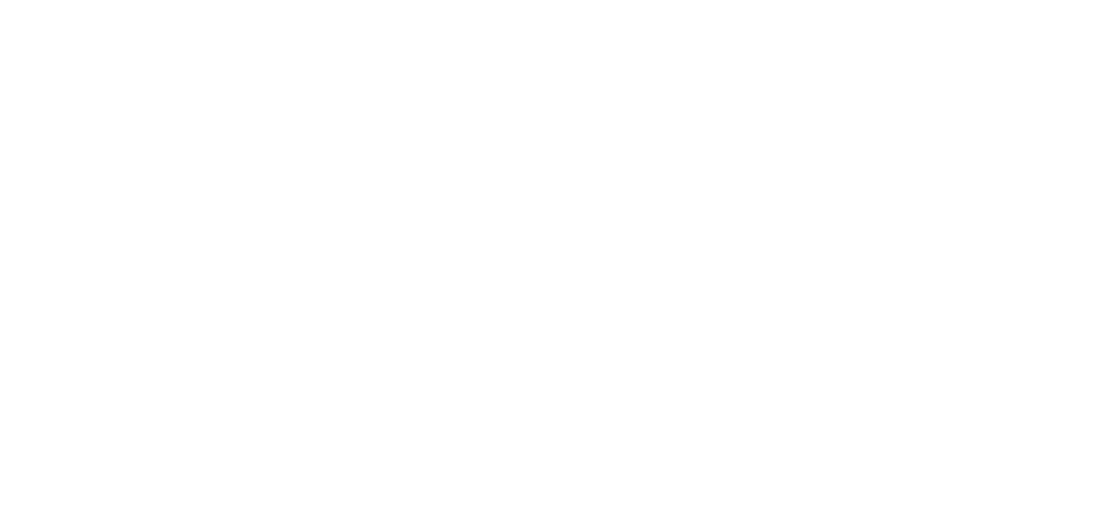
\includegraphics[width=0.8\paperwidth]{images/titolo}
			%		\noindent {\fontsize{20.74}{2}\selectfont
				%		\bfseries\textcolor{white}{Elisa Antuca\ \ \ Massimo Bertolotti}}
		\end{center}
	\end{textblock}
	
	
	
	\begin{textblock}{.9}(.05,.56)
		\begin{flushright}
			\noindent {\fontsize{20.74}{2}\selectfont
				\bfseries\textcolor{white}{Manualozzo\texttrademark\  di Fisica 2}}
		\end{flushright}
	\end{textblock}
	
	
	\begin{textblock}{.45}(.55,.705)
		\begin{center}
			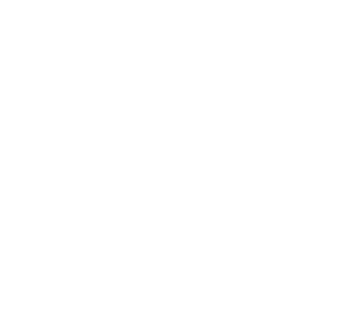
\includegraphics[width=.35	\paperwidth]{images/copertina2}
		\end{center}
	\end{textblock}
	
	\begin{textblock}{.1}(-.005,.59)
		\begin{center}
			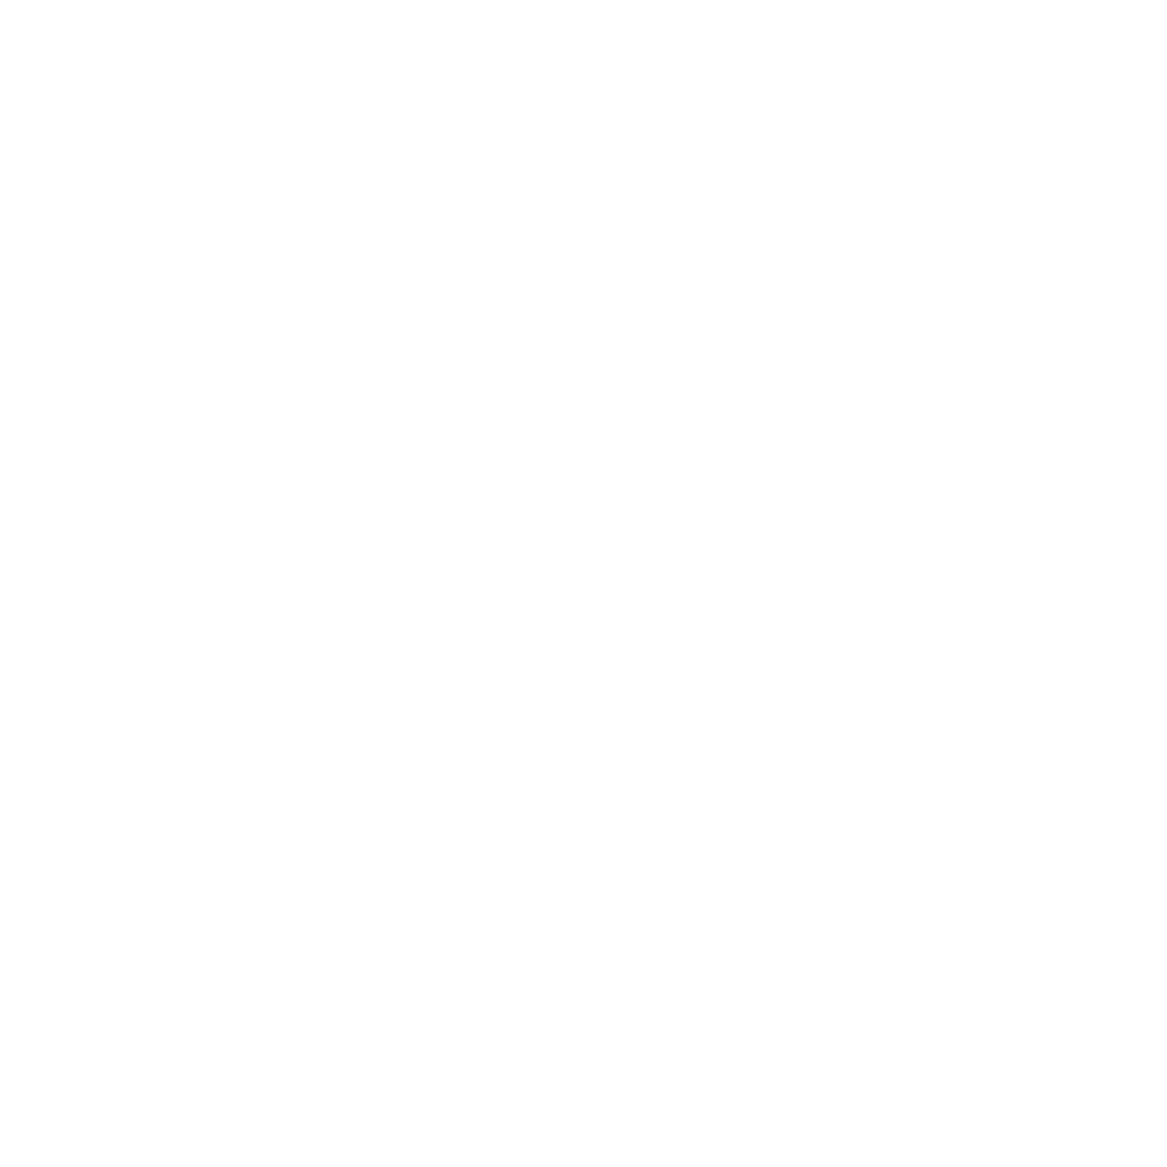
\includegraphics[width=.38\paperwidth]{images/copertina3}
		\end{center}
	\end{textblock}
	
	\begin{textblock}{.45}(.86,.69)
		\noindent {\fontsize{24.74}{18}%
			\textcolor{white}{$\displaystyle E=mc^2$}}
		%\begin{center}
		%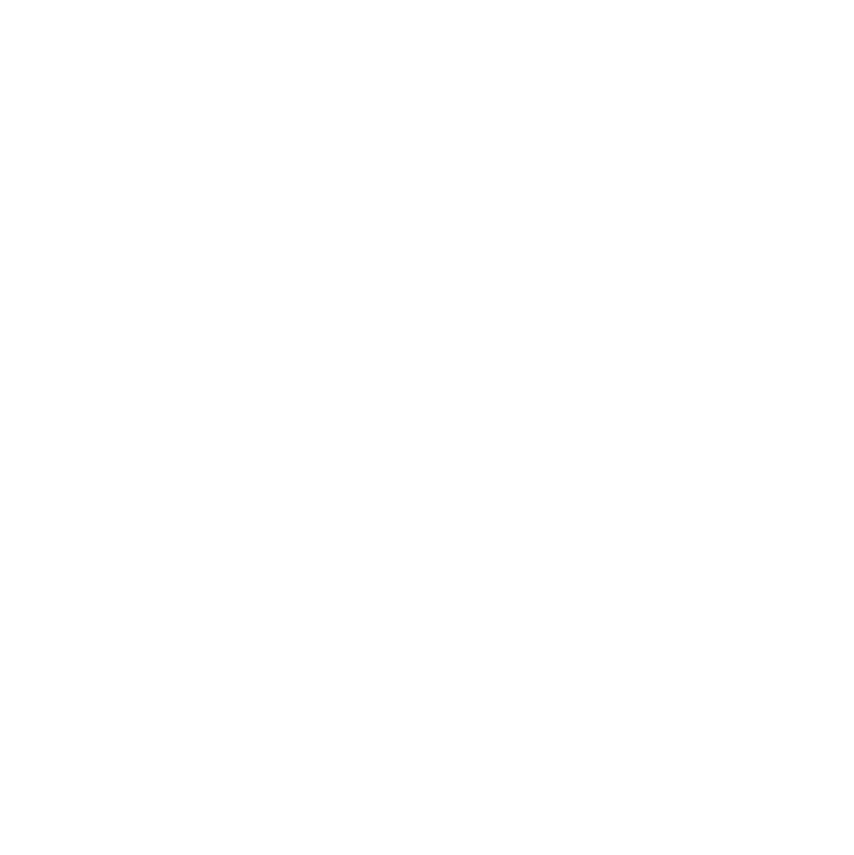
\includegraphics[width=.15\paperwidth]{images/copertina4}
		%\end{center}
	\end{textblock}
	
	\begin{textblock}{.4}(.3,.35)
		\begin{center}
			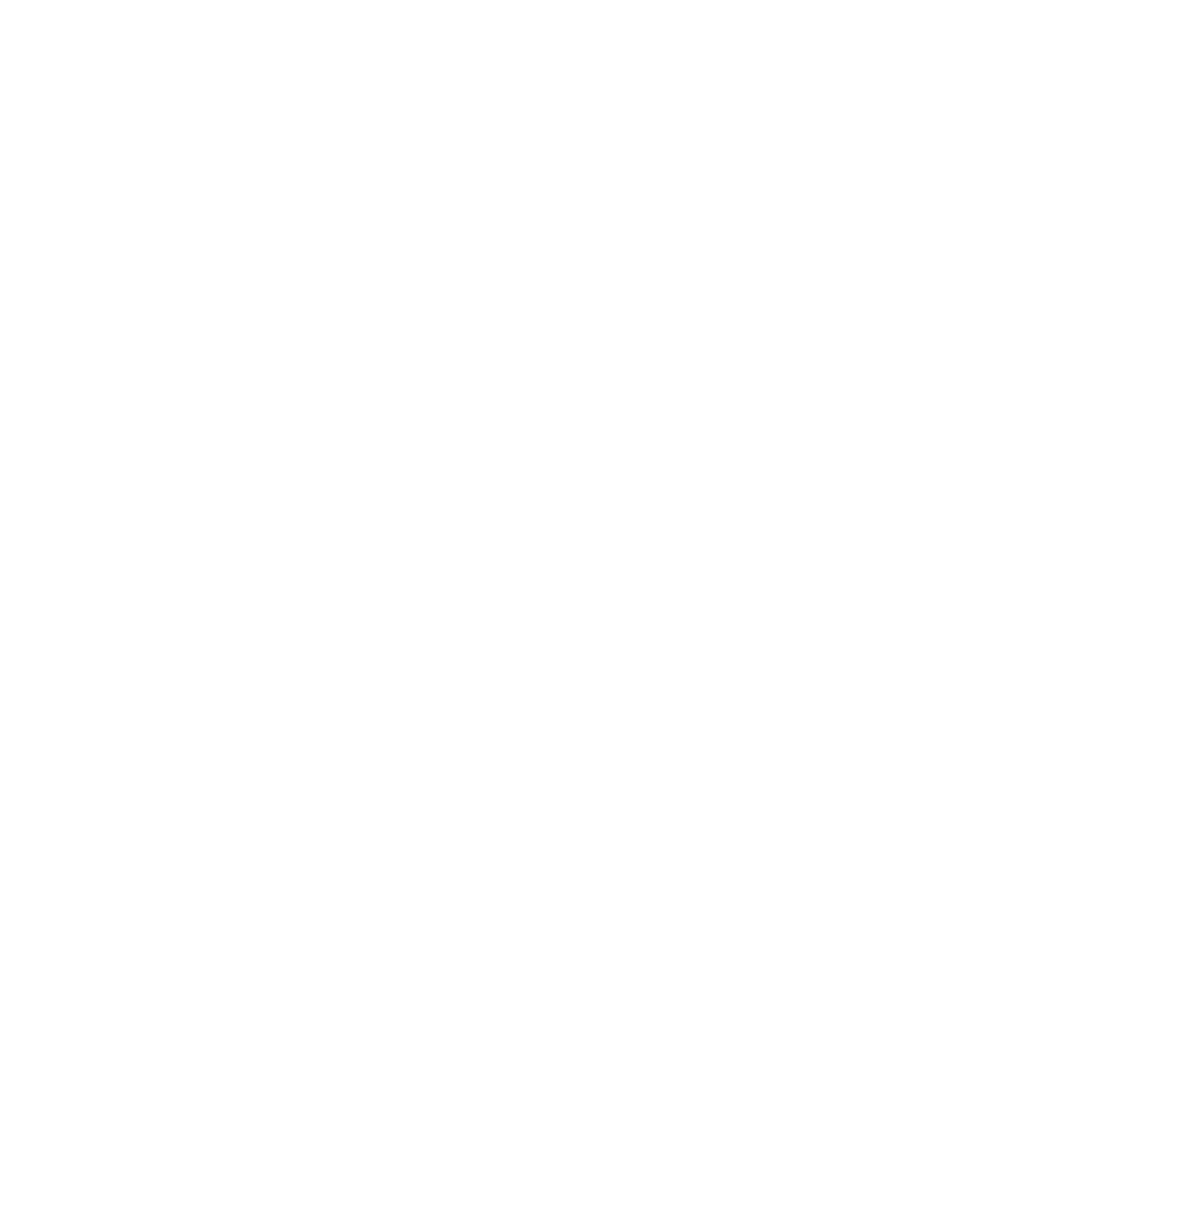
\includegraphics[width=.2\paperwidth]{images/unitologo}
		\end{center}
	\end{textblock}
	
	\begin{textblock}{.6}(.1,.58)
		\noindent {\fontsize{14.74}{18}%
			\textcolor{white}{$\displaystyle\vba{F}=q\left(\vba{E}+\vba{v}\cross\vba{B}\right)$}}
	\end{textblock}
	
	
	\begin{textblock}{.3}(.245,.86)
		\noindent {\fontsize{15.28}{18}%
			\textcolor{white!80}{$\displaystyle\lim_{n\to+\infty}\int_Xf_nd\mu=\int_X\lim_{n\to+\infty}f_nd\mu$}}
	\end{textblock}
	
	\begin{textblock}{.4}(.05,.91)
		\noindent {\fontsize{14.4}{18}%
			\textcolor{white!50}{$\displaystyle \mu\left(\bigcup_{n\geq 1}A_n\right)=\lim_{n\to+\infty}\mu\left(A_n\right)$}}
	\end{textblock}
	
	\begin{textblock}{.6}(.36,.605)
		\begin{center}
			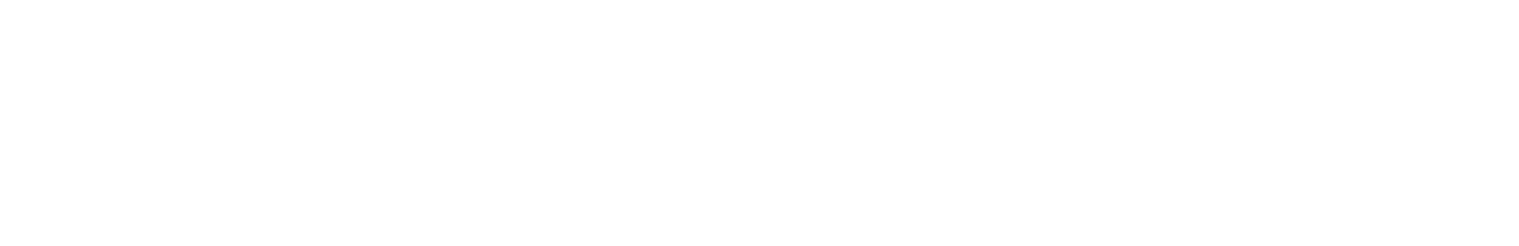
\includegraphics[width=.575\paperwidth]{images/copertina1}
		\end{center}
	\end{textblock}
	
	
	\begin{textblock}{.3}(.34,.75)
		\noindent {\fontsize{16.28}{18}%
			\textcolor{white!10}{$\displaystyle \curl{\vba{B}}=\mu_0\left(\vba{j}+\epsilon_0\pdv{\vba{E}}{t}\right)$}}
	\end{textblock}
	
	
	
	\null\newpage
\end{comment}
\begin{comment}
	\begin{center}
	\newlength{\parSepLength}
	\setlength{\parSepLength}{10ex}
	
	\Large
	\centering
	
	% Main title
	\thinRule\par
	\par\vspace{0.15\parSepLength}
	\begin{minipage}{\textwidth}
	\centering
	\fontsize{40pt}{36pt}\selectfont\titleColor\scshape
	Appunti di Geometria 2
	\end{minipage}
	\par\vspace{0.25\parSepLength}
	\par\thinRule
	
	\vspace{0.125\parSepLength}
	
	\begin{minipage}{\textwidth}
	\centering
	\small
	Anno Accademico 2020/2021
	\end{minipage}
	
	\vspace{0.225\parSepLength}
	
	\begin{minipage}{\textwidth}
	\centering
	‘‘Un matematico è una macchina per trasformare caffè in teoremi.''\\
	Alfréd Rényi
	\end{minipage}
	
	\vfill
	
	% Author
	\begin{minipage}{\textwidth}
	\centering
	%\Large
	\begin{center}
	\includegraphics[width=0.25\linewidth]{images/Unito-logo}
	\end{center}
	
	\end{minipage}
	
	\vfill
	
	% Logo and other info
	% \begin{minipage}{0.8\textwidth}
	%    \centering
	%    \small
	
	% Examiner
	%    \begin{minipage}[t]{0.29\textwidth}
	%      \textsc{Titolari del corso} \\
	%     {\scriptsize Prof. Marco Costa\\
	%      Prof. Antonaldo Diaferio\\
	%       Università di Torino}
	%    \end{minipage}
	%   \hfill
	% Supervisor
	%   \begin{minipage}[t]{0.26\textwidth}
	%      \begin{center}
	%     	\textsc{Adattamento \LaTeX} \\ 
	%     \textsc{e integrazioni discutibili} \\
	%     {\scriptsize Massimo Bertolotti\\
	%      Università di Torino}
	%     \end{center}
	%   \end{minipage}
	%	\hfill
	%	\begin{minipage}[t]{0.27\textwidth}
	%	\raggedleft
	%	\textsc{Revisione contenutistica} \\ 
	%	{\scriptsize Elisa Antuca\\
	%	 Università di Torino}
	%	\end{minipage}
	%  \end{minipage}
	\end{center}
\end{comment}
\afterpage{\blankpage}
%% SVN info for this file
\svnidlong
{$HeadURL$}
{$LastChangedDate$}
{$LastChangedRevision$}
{$LastChangedBy$}

\chapter*{Introduzione al Manualozzo\texttrademark\ }
\labelChapter{introduzione}

\begin{introduction}
‘‘Sai, per essere un matematico non aveva abbastanza immaginazione; ma ora è diventato un poeta e se la cava davvero bene.''
\begin{flushright}
	\textsc{David Hilbert,} riferendosi \Ccancel[red]{a Marino Badiale} all'autore del Manualozzo\texttrademark\ .
\end{flushright}
\end{introduction}
{\small 
\noindent Guardando la copertina di questo testo, dei potenziali lettori - sì, parlo con voi - si potrebbero chiedere: ‘‘Ma che diamine è un \textit{Manualozzo\texttrademark\ }?''
\vspace{3mm}
\lettrine[findent=1pt, nindent=0pt]{\textbf{M}}{\textbf{anualozzo\texttrademark\ }} s. m. [der. di \textit{manuale}, col suff. \textit{-ozzo}]. - Appunti di lezioni universitarie scritti da studenti, senza troppe pretese di formalità e potenzialmente non totalmente corretti, ma sono comunque meglio che niente.\footnote{Nota per l'ufficio legale: il \texttrademark\ in Manualozzo\texttrademark\ non è legalmente vincolante - per il momento.}
\vspace{3mm}\\
Dunque, quello che state leggendo è il \textbf{Manualozzo\texttrademark\  di Fisica 2}, appunti a quattro mani basati sull'omonimo corso tenuto dai docenti Lorenzo Bianchi e Lorenzo Magnea nell'a.a. 2021-2022 presso il Dipartimento di Matematica dell'Università degli Studi di Torino.\\
Questo testo ripercorre le scoperte scientifiche e le rivoluzioni epistemologiche che caratterizzarono la fisica dell'Ottocento e dei primi del Novecento. \\
Nella prima parte raggiungeremo l'\textit{apice} della \textit{Fisica classica}, esplorando estensivamente una delle sue teorie più raffinate, l'\textbf{elettromagnetismo}; a ciò segue un breve ma fondamentale excursus sulle \textbf{onde} (elettromagnetiche).\\
Invece, nella seconda parte metteremo in \textit{crisi} quanto visto prima: partendo da alcune incongruenze irrisolvibili con la Fisica classica, introdurremo la teoria della \textbf{relatività speciale} e alcuni cenni di \textbf{fisica quantistica}.\\
I prerequisiti necessari sono gli argomenti trattati nei corsi di \textsc{Analisi Matematica Uno}, \textsc{Due} e \textsc{Fisica Uno} - con qualche nozione di \textsc{Geometria 3} e \textsc{Meccanica Razionale}.\\
Ma il \textit{Manualozzo\texttrademark\ } non è una mera sbobinatura delle lezioni: in aggiunta agli argomenti trattati nella teoria, potrete trovare a fine libro delle utili \textit{postille} con alcune digressioni interessanti, nonché tabelle ed elenchi riepilogativi dei teoremi, delle definizioni e delle proprietà affrontate - il tutto, ovviamente, in Technicolor\texttrademark. %{\small Seriamente, dove abbiamo trovato il tempo per fare tutto, qualcuno ce lo dica.}
Purtuttavia, ci duole ammetterlo, gli autori non sono \textit{esseri infallibili}: saranno sicuramente sfuggiti degli errori (o degli \textit{orrori}, la cui causa è solamente degli autori che non hanno studiato bene e assolutamente non dei professori), per cui ogni segnalazione - direttamente agli autori se ancora in vita oppure su \textcolor{redill}{\url{https://maxmaci.github.io}} - è ben gradita, in modo da migliorare le future edizioni del \textit{Manualozzo\texttrademark\ }.}

\vfill
\begin{center}
	Prima edizione, compilato il \today.\\
			
\includegraphics[trim=0cm 0cm 0cm 0cm,clip,scale=0.5]{images/Cc-by-nc-sa_icon.pdf}\\
	{\footnotesize This work is licensed under a \href{https://creativecommons.org/licenses/by-sa/4.0/}{Attribution-NonCommercial-ShareAlike 4.0 International.}}
\end{center}
\newpage
\section*{Note per gli environment}
Se alcuni professori sono noti per abusare le notazioni, i Manualozzi sono noti per abusare di \textit{environment} - gli ambienti colorati che vedrete in queste pagine; di seguito ci sono alcune informazioni su di essi.

\noindent\textit{Teoremi}, \textit{proposizioni}, \textit{lemmi} e \textit{corollari} possono essere seguiti da una \textit{dimostrazione}, come nell'esempio di seguito...
\begin{theoremanote}[Cardinalità dei razionali]
	Ci sono più numeri razionali che interi.
\end{theoremanote}
\begin{demonstration}
	La dimostrazione si basa sulla congettura che tutti gli interi siano razionali; mostriamo il teorema per $0$, gli altri $\aleph_0$ casi sono analoghi.\\
	Dato $0$, basta prendere $\nicefrac{1}{2}$: questo è banalmente un razionale - convincetevi che questo sia vero! In questo modo, abbiamo trovato due razionali di cui uno non intero.
\end{demonstration}
... oppure essere forniti \textit{senza} dimostrazione e quindi nell'enunciato troverete alla fine il simbolo $\square$:
\begin{corollarynote}[Ultimo teorema di Fermat]
	Sulla base del teorema precedente vale immediatamente per confronto l'ultimo teorema di Fermat.
\end{corollarynote}
Nelle sezioni ‘‘Eserciziamoci!'' potrete invece trovare esercizi con corrispettive soluzioni: sono simili talvolta a dei risultati teorici, ma tendono ad essere più applicativi.

\noindent Alcuni degli \textit{environment} più comuni dopo questi sono le \textit{osservazioni} e gli \textit{esempi}, che sono autoesplicativi. Ci sono anche altri \textit{environment}, meno comuni, fra cui...
\begin{digression}
	Sono argomenti \textit{non prettamente trattati} in questo corso che, tuttavia, hanno un legame con esso: possono \textit{aggiungere informazioni} e punti di vista a qualcosa visto nei corsi precedenti oppure fornire delle \textit{anticipazioni} per dei corsi futuri.
\end{digression}
\begin{attention}
	Sono delle osservazioni mirate e rivolte spesso a segnalare \textit{errori} frequenti, dovuti principalmente a proprietà che \textit{non} si verificano in quel dato tangente. 
\end{attention}
\begin{intuit}
	Sono delle interpretazioni \textit{euristiche} di una definizione difficile o di un risultato ostico che possono aiutare a capire il perché di tale cosa - per quanto non siano sempre valide a livello formale. 
\end{intuit}
\section*{Note per gli elenchi delle definizioni e dei teoremi}
In fondo al Manualozzo si possono trovare degli elenchi con tutte le definizioni, assiomi e risultati teorici visti: ognuno di essi è indicato nel formato \textbf{\textsc{X\#.\#.\#. TITOLO}}, dove \textbf{\textsc{X}} è una \textit{sigla} per indicare il tipo di definizione/risultato, mentre \textbf{\textsc{\#.\#.\#.}} individua il \textit{capitolo}, la \textit{sezione} e il \textit{numero} per quell'oggetto nella sezione. I significati delle sigle sono elencati di seguito:
\begin{multicols}{2}
	\begin{itemize}
		\item \textbf{\textsc{A}}: Assioma.
		\item \textbf{\textsc{D}}: Definizione.
		\item \textbf{\textsc{T}}: Teorema.
		\item \textbf{\textsc{PR}}: Proposizione.
		\item \textbf{\textsc{L}}: Lemma.
		\item \textbf{\textsc{C}}: Corollario.
		\item \textbf{\textsc{PT}}: Proprietà.
	\end{itemize}
\end{multicols}



%% SVN info for this file
\svnidlong
{$HeadURL$}
{$LastChangedDate$}
{$LastChangedRevision$}
{$LastChangedBy$}

\tableofcontents

\mainmatter
% TO DO: proposta: riordinare come il mazzoldi: forza e campo elettrostatico, potenziale elettrostatico, legge di Guass ed elettrostatica.
\part{Elettrostatica}
\labelPart{first}
% SVN info for this file
\svnidlong
{$HeadURL$}
{$LastChangedDate$}
{$LastChangedRevision$}
{$LastChangedBy$}

\chapter{Dalla legge di Coulomb al formalismo dei campi vettoriali}
\labelChapter{ellipseintroduction}

\begin{introduction}
‘‘Per ogni problema c'è una soluzione che è semplice, chiara... e sbagliata.''
\begin{flushright}
	\textsc{Henry Louis Mencken} ad un suo studente che trovò come perimetro dell'ellisse $\pi ab$. % TO DO: quote 
\end{flushright}
\end{introduction}
\lettrine[findent=1pt, nindent=0pt]{L}{a meccanica} ci descrive come funziona un sistema soggetto ad una certa \textit{forza}. Ad oggi, siamo riusciti a ricondurre tutte le forze ad alcune \textbf{interazioni fondamentali}; in ordine di magnitudine decrescente:
 \begin{itemize}
 	\item (Nucleare) Forte.
 	\item Elettromagnetica.
 	\item (Nucleare) Debole
 	\item Gravitazionale
 \end{itemize}
\parshape=0 Wow, sono \textit{davvero} poche! Dov'è la frizione, la forza elastica, le reazioni vincolari, le forze chimiche che legano le particelle, gli urti tra palle del biliardo? Che ci crediate o no, \textit{tutte} queste forze sono elettromagnetiche. E le altre interazioni fondamentali che fine fanno?

Le \textbf{interazioni (nucleari) forti} tengono uniti i \textit{quark} che costituiscono neutroni e protoni, nonché legano assieme protoni e neutroni nel \textit{nucleo atomico}, ma agiscono su una scala così piccola che risultano essere completamente impercettibili - pur essendo centinaia di volte più forti delle forze elettromagnetiche!\\
Le \textbf{interazioni (nucleari) deboli}, che riguardano certi procedimenti di decadimenti nucleari, hanno un nome autoesplicativo: sono forze a microscopico raggio d'azione \textit{e} sono più deboli delle forze elettromagnetiche.\\
Non parliamo poi della \textbf{interazione gravitazionale}: essa è terribilmente debole nonostante abbia un \textit{range} d'azione infinito, e la notiamo solamente in presenza di grandi, \textit{enormi} concentrazioni di massa - i pianeti e le stelle. Se al posto delle forze elettriche l'atomo fosse tenuto assieme da forze gravitazionali, un singolo atomo di idrogeno sarebbe più grande dell'intero universo osservabile.

Quindi, non solo le \textbf{forze elettromagnetiche} sono quelle dominanti nella vita di tutti i giorni (sono potenti \textit{e} hanno un \textit{range} d'azione infinito), ma sono anche le sole che \textit{al momento} sono completamente spiegate da una teoria. Certo, c'è una teoria gravitazionale classica e relativistica, ma non ne esiste una soddisfacente in campo quantistico; per le forze deboli c'è una teoria popolare, ma ostica, e per le forti si sta facendo strada la \textit{cromodinamica}... eppure, nessuna di queste teorie può vantare una verifica sperimentale definitiva. La cosa curiosa è che tutte queste teorie sperimentali si rifanno al modello perfetto, da emulare, delle \textit{leggi (classiche) dell'elettromagnetismo}.

Anche se le prime osservazioni sui fenomeni elettromagnetici sono attribuite al filosofo greco Talete nel VI secolo a.C., fu grazie alle innumerevoli scoperte di Franklin, Coulomb, Ampère, Faraday, Volta e tanti altri che \textbf{James Clerk Maxwell} impacchettò tutto questo bagaglio scientifico in quattro, stupende formule matematiche - che probabilmente avrete visto per la prima volta su una discutibile maglietta di un fan sfegatato della Fisica.

Prima di arrivare a formulare tutte le equazioni di Maxwell, tuttavia, ci conviene fare un tour guidato attraverso la storia di questa disciplina, costruendo passo per passo queste leggi facendo le stesse osservazioni dei più famosi scienziati che lavorarono sull'elettromagnetismo - chiaramente, viste con degli strumenti matematici moderni. In questo capitolo, dopo un'excursus storico dello studio dei fenomeni elettrostatici introdurremo la \textbf{legge di Coulomb}; la seconda parte sarà più prettamente matematica e tratterà del \textbf{formalismo dei campi vettoriali} - introducendo diversi strumenti particolarmente utili ai nostri scopi.
\section{I primi studi dell'elettricità}
Già, ma... che significa il termine \textbf{‘‘elettromagnetismo''}? La sua etimologia permette di svelare molte informazioni su come stati osservati in natura questi fenomeni:
\begin{itemize}
	\item ‘‘Elettro'' e ‘‘elettricità'' derivano da \textit{elettricus}, parola latina coniata nel 1600 da \textbf{William Gilbert} nel suo trattato \textit{De Magnete}, derivata a sua volta dal termine \textit{elektron}, ‘‘ambra'' in greco: infatti, le popolazioni attorno al Mediterraneo sapevano che oggetti in ambra, se strofinati con il pelo di gatto o col vello di lana, erano in grado di attrarre oggetti leggeri come piume e pagliuzze.
	\item ‘‘Magnetismo'' deriva da \textit{magnētis lithos}, ‘‘pietra di Magnesia'' in greco: sull'isola egea di Magnesia erano diffuse rocce di \textit{magnetite}, un minerale ferroso che in certi casi è capace di attrarre piccoli pezzetti di ferro.
\end{itemize}
\paragraph{Elettrizzazione per strofinio}
Il già citato Gilbert fu il primo a dare un certo rigore allo studio di questi fenomeni. Sperimentando sistematicamente con vari materiali, egli descrisse gli effetti delle \textbf{azioni elettriche per strofinio}\index{elettrizzazione per strofinio} - anche noto come \textbf{effetto triboelettrico}) - come segue:\\
\begin{minipage}{0.65\textwidth}
\begin{enumerate}[label=\alph*)]
	\item Due oggetti della \textit{stessa sostanza}, dopo essere stati strofinati da un panno, si \textit{respingono} se sono vicini l'un l'altro.
	\item Due oggetti di \textit{sostanze diverse} possono \textit{attrarsi} o \textit{respingersi}, a seconda dei materiali presi; ad esempio, vetro e ambra si attraggono.
	\item Due oggetti che sono attratti separatamente da un terzo oggetto si respingeranno a vicenda.
	\item Un oggetto è attratto da un materiale e un'altro oggetto è respinto da quel materiale, allora i due oggetti si attraggono tra di loro.
\end{enumerate}
\end{minipage}\hspace{10pt}
\begin{minipage}{0.34\textwidth}
		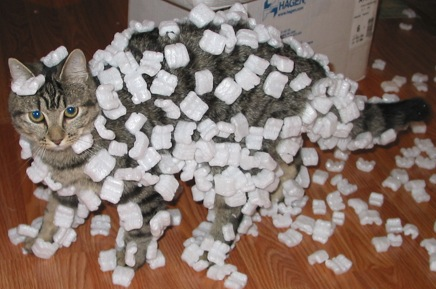
\includegraphics[width=1\textwidth]{images/foamcat.jpg}
	{\footnotesize Gilbert controllò tante combinazioni di materiali, ma non ‘‘pelo di gatto'' e ‘‘polistirolo da imballaggio''. Immagino non avesse un gatto per farlo.}
\end{minipage}\vspace{3pt}\\
Da queste osservazioni Gilbert concluse l'esistenza di due tipi diversi di elettrizzazione, attribuite a \textbf{cariche elettriche}\index{carica elettrica} differenti.
\begin{define}[Carica elettrica positiva e negativa]
	Convenzionalmente, si dice che:
	\begin{itemize}
		\item Corpi come il vetro acquisiscono carica elettrica \textbf{positiva}\index{carica elettrica!positiva}, indicata con il segno più ($+$).
		\item Corpi come l'ambra acquisiscono carica elettrica \textbf{negativa}\index{carica elettrica!negativa}, indicata con il segno meno ($-$).
	\end{itemize}
Sintetizzando quanto detto:
\begin{itemize}
	\item Cariche elettriche \textit{dello stesso segno} ($+/+,\ -/-$) si \textbf{respingono}.
	\item Cariche elettriche \textit{di segno opposto} ($+/-$) si \textbf{attraggono}.
\end{itemize}
\end{define}
Il buon vecchio Gilbert si accorse anche che, seppur esistevano materiali (ambra, vetro, ebanite, bachelite...) che venivano elettrizzati per strofinio, altri (metalli, il corpo umano...)\textit{non} venivano proprio elettrizzati. I primi li chiamò \textbf{isolanti}\index{isolante}, i secondi \textbf{conduttori}\index{conduttore}.
\paragraph{La struttura della materia e i fenomeni elettrostatici}
Gilbert scrisse per bene tutte queste osservazioni nel suo trattato \textit{De Magnete}, scritto nel 1600: all'epoca non poteva spiegare \textit{perché} succedeva ciò che aveva descritto, ma noi grazie alla conoscenza della \textit{struttura microscopica della materia} possiamo farlo. Senza perderci in tanti dettagli, la materia è fatta di \textbf{atomi}\index{atomo}, tutti costituiti da tre particelle: \textbf{protoni} $p$, \textbf{neutroni} $n$ ed \textbf{elettroni} $e$, rispettivamente di massa
\begin{itemize} % TO DO: simboli SI
	\item $m_p = 1,6725 \cdot 10^{-27}\ $ 
	\item $m_n = 1,6748\cdot 10^{-27}\ $
	\item $m_e = \frac{1}{1840}m_p=9,1091\cdot 10^{-31}\ $
\end{itemize}
Riprendendo la convenzione precedente, si vede che il protone ha carica \textit{positiva}, mentre l'elettrone ha carica \textit{negativa} e il neutrone non ha carica elettrica; ad oggi non è osservata alcuna carica elettrica più piccola di quella del protone o dell'elettrone - in altre parole, la carica elettrica è una grandezza \textbf{quantizzata}\footnote{La quantizzazione della carica è evidente a livello atomico e subatomico, ma diventa inapprezzabile se la non riescono a misurare variazioni dell'ordine della carica elementare - sperimentalmente si è visto intorno per carica sopra i $200 e$. Negli esperimenti normali di elettrostatica la carica è di fatto una quantità continua.}. Indicheremo con $-e$ la carica dell'elettrone e, in virtù della quantizzazione della carica elettrica, la chiameremo \textbf{carica elementare}\index{carica!elementare}, mentre con $+e$ indicheremo la carica del protone.

Il \textbf{nucleo}\index{nucleo}, costituito da protoni e neutroni, sta saldamente assieme grazie all'interazione nucleare forte che sovrasta le azioni repulsive delle cariche positive, che tra l'altro rendono il nucleo \textit{carico positivo}. Attorno al nucleo orbitano, attratte da forze elettriche, gli \textit{elettroni}: queste particelle sono in numero pari al numero di protoni nel nucleo e, a differenza di essi, sono molto più liberi di muoversi nello spazio circostante il nucleo. Si osserva che l'atomo è, nel suo complesso, \textit{elettricamente neutro}, dato che la carica del protone e dell'elettrone è uguale in modulo e la carica complessiva. Questo è estremamente importante per la struttura della materia; se non ci fosse questa \textit{cancellazione}\footnote{Per cancellazione non intendiamo che le carica si annichiliscono fisicamente, ma che i loro effetti si compensano, non producendo alcuna interazione ‘‘esterna''.} della carica, saremmo soggetti a forze estreme: una patata esploderebbe violentemente se ci fosse anche solo una cancellazione imperfetta dell'ordine di una parte su $10^10$.

Sostanze diverse hanno legami più o meno deboli tra il nucleo e gli elettroni, in particolari quelli periferici. Cosa succede, a livello microscopico, con l'elettrizzazione per strofinio? Il \textbf{contatto} tra i due corpi trasferisce \textit{per mezzo meccanico} elettroni dello strato superficiale da un corpo all'altro, dal corpo in cui sono meno fortemente legati verso quello in cui lo sono di più.
\begin{itemize}
	\item Negli \textbf{isolanti}, le cariche trasferite per strofinio rimangono \textit{localizzate}. Gli isolanti \textbf{non} trasportano facilmente la carica.
	\item Nei \textbf{conduttori}, le cariche elettriche negative sono \textit{libere di muoversi} e \textbf{non} rimangono localizzate. I conduttori trasportano facilmente la carica.
\end{itemize}
In altre parole, le forze elettriche sono una manifestazione fondamentale delle particelle atomiche (cariche) che costituiscono la materia, ma si manifestano a livello \textit{macroscopico} quando viene disturbata la simmetria naturale tra cariche positive e negative presenti negli atomi. Possiamo, in particolare, enunciare il seguente principio.
\begin{principle}[Principio della conservazione della carica]
	 Poiché la \textit{carica totale} di un corpo è data dalla \textit{somma algebrica} di tutte le cariche, in un sistema \textit{elettricamente isolato} la carica totale rimane costante nel tempo, ossia si \textit{conserva}.
\end{principle}
\paragraph{Induzione elettrostatica}
L'effetto triboelettrico che abbiamo visto è un caso particolare di \textbf{elettrizzazione per contatto}; tuttavia, si possono caricare corpi anche senza alcun contatto diretto, come accade con l'\textbf{induzione elettrostatica}\index{induzione elettrostatica}\\
Avviciniamo ad un \textit{conduttore} $C$, preso elettricamente scarico e sostenuto da un supporto isolante, un corpo carico $D$ - ad esempio, carico positivamente.
Il corpo carico esercita delle \textit{forze elettriche} sulle cariche microscopiche presenti sul conduttore; gli \textit{elettroni} nel conduttore sono liberi di muoversi sulla superficie e si dispongono nella zona di $C$ \textit{più vicina} al corpo carico, mentre la parte del conduttore più distante da $D$ risulterà carica positivamente\footnote{Chiaramente, se il corpo $D$ fosse carico negativamente accaderebbe l'opposto: gli elettroni in $C$ sarebbero respinti per l'interazione elettrica e si disporrebbero lontani dal corpo carico, rendendo positiva la zona vicina a $D$.}.
La carica complessiva del conduttore è, per conservazione della carica, sempre nulla, ma le cariche sono distribuite in modo non uniforme: convenzionalmente, pur essendo l'eccesso di cariche positive in una parte del conduttore dovuto al moto delle cariche negative, diremo che le cariche positive si sono spostate nella zona di $C$ a maggior distanza da $D$.

Se collegassimo il conduttore $C$ ad un conduttore $T$ molto più esteso di $C$, ad esempio la Terra, di fatto si creerebbe un unico conduttore $C+T$ praticamente infinito per i nostri scopi. In questo caso, le cariche positive si allontanerebbero molto da $D$; se interrompessimo il collegamento del conduttore a $T$ il conduttore $C$ resta carico negativamente - basta allontanare $D$ per ottenere $C$ negativo con distribuzione uniforme di carica.
\paragraph{Misura delle cariche elettriche: l'elettroscopio a foglie}
Abbiamo detto che la carica elettrica è una grandezza quantizzata... ma non abbiamo ancora parlato di come definirla esattamente, né di come \textit{misurarla}! Al momento, ne diamo una definizione operativa, tramite l'\textbf{elettroscopio a foglie}\index{elettroscopio a foglie}\\
Dato un contenitore isolante e trasparente si consideri un asta metallica che lo penetra in un foro in modo da rimanere bloccata. All'estremità inferiore, internamente al recipiente, sono appese due sottilissime foglioline metalliche - generalmente d'oro - liberi di ruotare attorno all'asse orizzontale dell'asta. Se l'asta metallica è scarica, le foglioline sono verticali per effetto della gravità.

Toccando l'asta con un corpo carico, essa si carica e parte della corrente posseduta dall'asta si dispone sulle foglioline. Poiché le foglioline sono cariche dello stesso segno, si respingono e divergono dalla verticale di un angolo $\alpha$ che può opportunamente misurato con una scala graduata: abbiamo creato uno strumento in grado di rilevare la presenza di cariche elettriche. Possiamo allora dare la seguente definizione \textit{operativa} di carica elettrica.
\begin{define}[Definizione operativa di carica elettrica]
Se due corpi uguali, toccando l'asta di un elettroscopio a foglie inizialmente scarico, fanno ruotare le foglioline di uno stesso angolo $\alpha$, allora hanno la stessa carica $q$.
\end{define}
Potremmo fornire già in questa maniera un'opportuna unità di misura, ma non è particolarmente utile e non è compatibile con la filosofia di molti sistemi di unità di misura. Tuttavia, per dare una possibile definizione \textit{non} operativa, dobbiamo quanto meno parlare dell'interazione elettrostatica.
\section{Legge di Coulomb}
Corpi carichi si attraggono o si respingono, a qualunque distanza, a seconda della loro carica: più sono vicini e più sono carichi, maggiore è questa attrazione/repulsione. Questa descrizione qualitativa delle forze di natura elettrostatica era già nota da Gilbert, ma per averne una \textit{quantitativa} dobbiamo aspettare quasi duecento anni.
Nel 1785, il fisico francese \textbf{Charles Augustin de Coulomb} pubblicò la sua memoria \textit{Recherches théoriques et expérimentales sur la force de torsion et sur l'élasticité des fils de metal}, in cui stabilì, mediante l'uso di una bilancia di torsione analoga a quella di \textit{Cavendish} per la misura delle forze gravitazionali, una legge matematica per la descrizione dell'interazione elettrostatica.
\begin{define}[Legge di Coulomb]\index{Legge!di Coulomb}
	Date due cariche puntiformi $q_1$ e $q_2$, poste a distanza $r$ \textit{nel vuoto}, interagiscono con una forza $F$ diretta secondo la loro congiungente data da
	\begin{equation}
		\vba{F}=k\frac{q_1q_2}{r^2}\vbh{u}_r\label{leggeCoulomb}
	\end{equation}
\end{define}
\begin{observes}~
	\begin{itemize}
		\item $\vba{F}$ è la forza che $q_1$ esercita su $q_2$; la forza che $q_2$ esercita su $q_1$ e $-\vba{F}$.
		\item $k$ è una costante di proporzionalità detta \textbf{costante di Coulomb}\index{costante!di Coulomb} che dipende dalle unità di misura.
		\item $\vbh{u}_r$ è il versore del vettore distanza $\vba{r}$ dalla carica $q_1$ alla carica $q_2$.
		\item $q_1q_2$ è il prodotto delle due cariche: se hanno lo stesso segno, la forza è repulsiva perché $\vba{F}$ ha lo stesso verso di $\vbh{u}_r$, altrimenti se hanno segno opposto è attrattiva perché hanno versi discordi.
	\end{itemize}
\end{observes}
Non abbiamo ancora dato per bene un'unità di misura della carica elettrica. Potremmo basarci proprio sulla legge di Coulomb e definirla in modo che $k=1$ e che la carica unitaria è tale che, se posta a distanza unitaria da un'altra carica unitaria, essa subisce una forza unitaria (come accade nel \textit{sistema centimetro-grammo-secondo o c.g.s}).  

Nonostante alcuni evidenti vantaggi teorici nell'utilizzare il sistema c.g.s., noi utilizzeremo per ragioni anche soprattutto storiche, l'unità di misura della carica elettrica prevista dal \textbf{SI}, il \textbf{coulomb}\index{coulomb} ($\ $). % TO DO: add unit box
Non è un'unità fondamentale, bensì è definito come $\ \cdot \ $, ossia come la carica che attraversa in un secondo un conduttore percorso dalla corrente di un ampere. Non sapendo ancora che cosa sia la corrente elettrica, né tanto meno un'ampere, non approfondiremo qui la definizione.

Sta di fatto che è una misura estremamente ‘‘sbagliata'', quanto meno per i problemi che trattiamo. Ad esempio, la tipica carica da strofinamento è dell'ordine di $10^{-7}\ $ - dobbiamo impegnarci molto per fare un Coulomb! Generalmente utilizziamo i microcoulomb ($\ $) o, al più, i millicoulomb ($\ $).\\
Nel \textbf{SI}, la costante $k$ della legge di Coulomb viene posta a
\begin{equation}
	k=\frac{1}{4\pi\epsilon_0}=8,9875\cdot 10^9\ \frac{\ }{\ \cdot \ }
\end{equation}
dove $\epsilon_0$ è detta \textbf{costante dielettrica del vuoto}\index{costante!dielettrica del vuoto} e assume il valore
\begin{equation}
	\epsilon_0=8,854\cdot 10^{-12}\ \frac{\ }{\ \cdot \ }
\end{equation}
La legge di Coulomb \ref{leggeCoulomb} assume la forma
\begin{equation}
\vba{F}=\frac{1}{4\pi\epsilon_0}\frac{q_1q_2}{r^2}\vbh{u}_r
\end{equation}
\paragraph{Legge di Coulomb e legge di gravitazione universale}
Come si vede immediatamente, la legge di Coulomb è analoga - a livello di formula - alla \textbf{legge di gravitazione universale}:
\begin{equation}
	\vba{F}=G_N\frac{m_1m_2}{r^2}\vbh{u}_r
\end{equation}
dove $G_N$ è la \textbf{costante di gravitazione universale}\index{costante!di gravitazione universale}.
\begin{equation}
	G_N=6,7\cdot 10^{-11}\ \frac{\ }{\ \cdot \ }
\end{equation}
Tuttavia, a livello di forze sono profondamente differente, come il seguente esempio mette in evidenza.
\begin{example}
	La forza di Coulomb tra due cariche uguali per strofinio, poste a distanza di $r=1\ =10^{-2}\ $ è, in modulo
	\begin{equation*}
		F=k\frac{q^2}{r^2}\simeq9\cdot 10^9\cdot 10^4\cdot 10^{-14}\ \simeq 0,9\ 
	\end{equation*}
	La forza gravitazionale in condizioni simili, prese due masse $m=1\ =10^{-1}\ $ alla stessa distanza $r$ di prima, è
	\begin{equation*}
		F=G_n\frac{m^2}{r^2}\simeq 7\cdot 10^{-17}\cdot 10^4\cdot 10^{-2}\simeq 7\cdot 10^{-9}\ 
	\end{equation*}
La forza di attrazione gravitazionale è molto più debole della forza attrattiva elettrostatica!
\end{example}
\paragraph{Principio di sovrapposizione per forze}
Le forze elettriche agenti su una carica $q_0$ dovute alle cariche circostanti si comportano come vettori; è immediato supporre che vige un \textbf{principio di sovrapposizione}\index{principio di sovrapposizione}.
\begin{principle}[Principio di sovrapposizione per forze elettrostatiche]
	La forza elettrostatica agente su una carica $q_0$ da un sistema di cariche è data dalla somma vettoriale delle singole interazioni tra $q_0$ e ciascuna carica del sistema.
\end{principle}
\section{Formalismo dei campi vettoriali}
Il problema fondamentale che la teoria dell'elettromagnetismo vuole risolve è il seguente: se ho delle cariche elettriche \textit{qui}, magari muovendoli in giro, cosa succede a delle cariche \textit{lì}?\\
La trattazione di un problema simile con le sole forze, come si farebbe in un qualunque corso di \textsc{Fisica I}, non è necessariamente la più vantaggiosa: in particolare, quando le cariche cominciano a muoversi, le forze tra di loro cambiano perché cambiano le posizioni nel tempo... e dovremo anche tenere conto degli effetti di magneti sul moto delle cariche!

È necessario un cambio di punto di vista, dove le forze ci sono ancora, ma non consideriamo \textit{soltanto} loro. La soluzione classica ottocentesca assume la forma di una \textbf{teoria di campo}. In estrema sintesi, lo spazio attorno ad una carica elettrica è permeata da campi elettrici e magnetici: una seconda carica, in presenza di questi campi, subisce una forza; i campi, in altre parole, trasmettono l'influenza di una carica sull'altra e sono i portatori dell'interazione elettromagnetica. I fenomeni elettromagnetici si modificano in base all'interazione tra i campi, le particelle in movimento e altro.
\begin{define}[Campo vettoriale]
	Un \textbf{campo vettoriale}\index{campo!vettoriale} $\vba{E}$ è una funzione
	\begin{equation}
		\funztot[\vba{E}]{\realset^3}{\realset^3}{(x,y,z)}{(E_x(x,y,z),E_y(x,y,z),E_z(x,y,z))}
	\end{equation}
dove $(x,y,z)$ sono eventualmente funzioni del tempo.
\end{define}
\begin{notate}
	In notazione versoriale, un campo vettoriale è
	\begin{equation}
		\vba{E}(x,y,z)=E_x\vbh{u}_x+E_y\vbh{u}_y+E_z\vbh{u}_z
	\end{equation}
\end{notate}
\begin{observe}
	Con $\vba{E}$ indichiamo il \textbf{campo elettrico}, mentre indichiamo con $\vba{B}$ il \textbf{campo magnetico}.
\end{observe}
\paragraph{Linee di campo}
Potremmo rappresentare il campo disegnando ad ogni punto di $\realset^3$ il vettore ad esso associato da $\vba{E}$.\\
In alternativa, possiamo disegnare delle curve dette \textbf{linee di campo}\index{linee di campo}.
\begin{define}[Linea di campo]
	Una linea di campo di $\vba{E}$ è una curva 
\begin{equation}
	\funztot[\gamma]{\realset}{\realset^3}{t}{\vba{r}(t)}
\end{equation}
tale per cui in ogni sup punto il vettore tangente alla curva è il vettore dato da $\vba{E}$:
\begin{equation}
	\dot{\gamma}(t)=\vba{E}\left(\gamma\left(t\right)\right),\ \forall t\in\realset
\end{equation}
\end{define}
In generale, le linee di campo sono soluzioni $\vba{r}=\left(x,y(x),z(x)\right)$ del sistema di equazioni differenziali
\begin{equation}
	\begin{cases}
		\frac{dy}{dx}=\frac{E_y}{E_x}\\
		\frac{dz}{dx}=\frac{E_z}{E_x}
	\end{cases}
\end{equation}
\section{Campo elettrostatico}
Un campo vettoriale è quindi una mappa che a punti di $\realset^3$ associa vettori tridimensionali.
In questo formalismo, la forza di Coulomb si può vedere come il vettore in un certo punto di un campo vettoriale detto \textbf{campo elettrostatico}.
\begin{define}[Campo elettrostatico]
	Il \textbf{campo elettrostatico}\index{campo elettrostatico} generato da un sistema di cariche $q_i$ ferme associa ad ogni punto dello spazio una forza pari alla forza elettrica che agisce su una \textbf{carica di prova}\index{carica!di prova} $q_0$ positiva posta in quel punto, divisa per la carica stessa:
	\begin{equation}\label{campoelettrostatico}
		\vba{E}(x,y,z)=\frac{\vba{F}}{q_0}=\frac{1}{4\pi\epsilon_0}\sum_i \frac{q_i}{\abs{\vba{r}-\vba{r_i}}^2}\vbh{u}_{r_i}=\frac{1}{4\pi\epsilon_0}\sum_i q_i\frac{\vba{r}-\vba{r_i}}{\abs{\vba{r}-\vba{r_i}}^3}
	\end{equation}
	dove $\vba{r}_i=(x_i,y_i,z_i),\ \vba{r}=(x,y,z)$ e $\vbh{u}_i=\frac{\vba{r}-\vba{r_i}}{\abs{\vba{r}-\vba{r_i}}}$.
\end{define}
Nel SI l'unitò di misura del campo elettrico, essendo il rapporto tra una forza e una carica, è il newton su coulomb ($\ / \ $). Più avanti vedremo un'altra unità di misura usata maggiormente nelle applicazioni pratiche.\\
Si noti che dalla definizione segue ovviamente che la forza che $q_0$ subisce si può esprimere in funzione del campo elettrostatico da
\begin{equation}
	\vba{F}=q_0\vba{E}
\end{equation}
Nella \ref{campoelettrostatico} abbiamo fatto uso di un \textbf{principio di sovrapposizione}\index{principio di sovrapposizione} per campi vettoriali.
\begin{principle}[Principio di sovrapposizione per campi elettrostatici]
	Il campo elettrico generato da un sistema di cariche è data dalla somma vettoriale dei campi elettrici generati da ciascuna carica del sistema.
\end{principle}
Preso il caso di una singola carica $Q$ posta nell'origine, il campo elettrico generato da $Q$ è
\begin{equation*}
	\vba{E}=\frac{1}{4\pi\epsilon_0}\frac{Q}{r^2}\vbh{u}_{r}=\frac{1}{4\pi\epsilon_0}Q\frac{\vba{r}}{r^3}=\frac{1}{4\pi\epsilon_0}\frac{Q}{(x^2+y^2+z^2)^{3/2}}(x,y,z)
\end{equation*}
\begin{examplewt}[Linee di campo della forza di Coulomb]
	Data una carica $Q$ post nell'origine del nostro sistema di rifermento, il campo elettrico di Coulomb nel piano è
	\begin{equation*}
		\vba{E}=\frac{1}{4\pi\epsilon_0}\frac{Q}{(x^2+y^2)^{3/2}}(x,y)
	\end{equation*}
Posto
\begin{gather*}
	dx=\dot{x}(t)=\frac{1}{4\pi\epsilon_0}Q\frac{x}{(x^2+y^2)^{3/2}}\\
	dy=\dot{y}(t)=\frac{1}{4\pi\epsilon_0}Q\frac{y}{(x^2+y^2)^{3/2}}
\end{gather*}
Da cui otteniamo la seguente equazione differenziale:
\begin{align*}
	\frac{dx}{dy}=\frac{x}{y}&\\
	\implies&\int_{x_0}^{x}\frac{dx}{x}=\int_{y_0}^{y}\frac{dy}{y}\implies \log\frac{x}{x_0}=\log\frac{y}{y_0}\implies y=\frac{y_0}{x_0}x
\end{align*}
Dalle condizioni al contorno $(0,0)$ e $(x_0,y_0)$ si ricavano le linee di forza del campo coulombiano: è un fascio di rette passanti per l'origine del sistema di riferimento.
\end{examplewt}
\begin{observe}
	Notiamo che la forza di Coulomb esercitata da una singola carica $Q$ posta nell'origine presenta un'evidente simmetria radiale; la stessa definizione \ref{leggeCoulomb} è già di fatto fornita in coordinate sferiche! Allora, il campo elettrostatico in coordinate sferiche è dato da
	\begin{equation*}
		\vba{E}=\frac{1}{4\pi\epsilon_0}\frac{Q}{r^2}\vbh{u}_{r}
	\end{equation*}
	ossia coincide con la componente radiale, dato che $E_\phi=E_\theta=0$.
\end{observe}
\section{Dipolo elettrico}
Consideriamo due cariche puntiformi $q_1$ e $q_2$, rispettivamente fisse in $\vba{r}_1=\left(0,0,z_0\right)$ e $\vba{r}_2=\left(0,0,-z_0\right)$. I campi elettrici generati dalle singole cariche sono, in un generico punto $\vba{r}=(x,y,z)$,
\begin{gather*}
	\vba{E}_1(x,y,z)=\frac{1}{4\pi\epsilon_0}\frac{q_1}{\abs{\vba{r}-\vba{r_1}^2}}\\
	\vba{E}_2(x,y,z)=\frac{1}{4\pi\epsilon_0}\frac{q_2}{\abs{\vba{r}-\vba{r_2}}^2}
\end{gather*}
Il campo elettrico complessivo è dato da
\begin{equation}
	\vba{E}(x,y,z)=\frac{1}{4\pi\epsilon_0}\left(q_1\frac{\vba{r}-\vba{r_1}}{\abs{\vba{r}-\vba{r_1}}^3}+q_2\frac{\vba{r}-\vba{r_2}}{\abs{\vba{r}-\vba{r_2}}^3}\right)
\end{equation}
Dato che
\begin{equation*}
	\begin{cases}
		\vba{r}-\vba{r}_1=\left(x,y,z-z_0\right)\\
		\vba{r}-\vba{r}_2=\left(x,y,z+z_0\right)
	\end{cases}
\end{equation*}
si ha
\begin{gather*}
	E_x(x,y,z)=\frac{1}{4\pi\epsilon_0}\left(q_1\frac{x}{(x^2+y^2+(z-z_0)^2)^{3/2y}}+q_2\frac{x}{(x^2+y^2+(z+z_0)^2)^{3/2}}\right)\\
	E_y(x,y,z)=\frac{1}{4\pi\epsilon_0}\left(q_1\frac{y}{(x^2+y^2+(z-z_0)^2)^{3/2}}+q_2\frac{y}{(x^2+y^2+(z+z_0)^2)^{3/2}}\right)\\
	E_z(x,y,z)=\frac{1}{4\pi\epsilon_0}\left(q_1\frac{z-z_0}{(x^2+y^2+(z-z_0)^2)^{3/2}}+q_2\frac{z_0}{(x^2+y^2+(z+z_0)^2)^{3/2}}\right)
\end{gather*}
Se consideriamo $q_1$ e $q_2$ di carica uguale a $q$ e di segno opposto (per esempio, $q_1=q$ e $q_2=-q$) abbiamo a che fare con il sistema detto \textbf{dipolo elettrico}\index{dipolo!elettrico}.
\paragraph{Momento di dipolo elettrico}
Al dipolo possiamo associare il \textbf{momento di dipolo elettrico}.
\begin{define}[Momento di dipolo elettrico]
	Il \textbf{momento di dipolo elettrico}\index{momento!di dipolo!elettrico} è una misura della separazione di cariche positive e negative in un sistema. In altre parole, misura la \textit{polarità} di un sistema elettrostatico.
	\begin{equation}
	\vba{p}=q\vba{d}
\end{equation}
dove $d$ è il vettore spostamento dalla carica negativa alla carica positiva-
\end{define}
Nel nostro caso, il modulo del momento di dipolo è $p=2qz_0$.
\begin{digression}
	Lo studio del dipolo elettrico è di particolare rilievo: ad esso sono riconducibili le interazioni elettrostatiche più semplici a cui sono soggetti i sistemi \textit{microscopici elettricamente neutri}, come atomi e molecole non ionizzate.\\
	Un esempio di ciò, anche se poco più complesso, è quello della molecola dell'acqua: è detta \textit{polare} in quanto gli elettroni condivisi sono distribuiti in modo non uniforme; c'è una concentrazione di carica negativa nel mezzo, presso l'atomo d'ossigeno, mentre agli estremi è positiva.\\
	Vedremo come il momento di dipolo ha particolare rilievo soprattutto quando la distanza tra le cariche è così piccola che non è facilmente misurabile, oppure quando parleremo di dielettrici.
\end{digression}
\paragraph{Studio del campo di dipolo}
Vogliamo descrivere il campo elettrostatico generato tramite vettori e tramite le linee di campo.
\begin{observe}
	Il sistema ha evidente natura \textit{cilindrica}: ci basterebbe studiare il comportamento su un piano passante per l'asse $z$ - ad esempio $y=0$; ciò che succede nello spazio si può capire con un'opportuna rotazione di tale piano.
\end{observe}
\begin{itemize}
	\item Consideriamo il piano $z=0$, ortogonale al dipolo e ‘‘a metà strada'' tra le due cariche.
	Chiaramente, $E_x=E_y=0$, dato che i denominatori sono uguali e i numeratori uguali, ma di segno opposto. Invece, si ha
	\begin{equation*}
		E_z=\frac{-2qz_0}{4\pi\epsilon_0}\frac{1}{\left(x^2+y^2+z_0^2\right)^{3/2}}
	\end{equation*}
	\item Consideriamo ora il piano $z=z_0$ e $y=0$. Si ha
	\begin{gather*}
		E_x=\frac{xq}{4\pi\epsilon_0}\left(\frac{1}{\abs{x}^3}-\frac{1}{\left(x^2+4z_0^2\right)^{3/2}}\right)\\
		E_y=0\\
		E_z=\frac{-2qz_0}{4\pi\epsilon_0}\frac{1}{(x^2+4z_0^2)^{3/2}}
	\end{gather*}
\end{itemize}
Analizzando ulteriori casi si denotano, per il dipolo elettrico, le linee di campo come in figura.
% TO DO: immagine
\begin{observe}
	Dove il campo elettrico è \textit{intenso}, la rappresentazione delle linee di campo è più densa, mentre si fa più rada dove il campo è \textit{meno intenso}.
\end{observe}
Se considerassimo $q_1=q_2=q$, le linee di campo sarebbero come quelle nella seguente figura.
% TO DO: immagine
\begin{observe}% TO DO: controllare se è l'opposto oppure no
	Dalle formule di dipolo, si vede che $\vba{E}$ è l'opposto del gradiente di un opportuno \textit{potenziale}\footnote{Nelle ‘‘XXX'', a pagina \pageref{gradiente} è possibile trovare la definizione di gradiente e altri operatori differenziali.} $V$:
	\begin{equation}
		V=-\frac{1}{4\pi\epsilon_0}\left(\frac{q_1}{\sqrt{x^2+y^2+(z-z_0)^2}}+\frac{q_2}{\sqrt{x^2+y^2+(z+z_0)^2}}\right)
	\end{equation}
Vedremo che questo \textit{non} è un caso: il potenziale elettrostatico è \textit{sempre} un campo \textit{conservativo}.
\end{observe}
\paragraph{Campo di dipolo lontano}
Cosa succede alle forze elettrostatiche e al campo elettrostatico se lo si osserva \textit{a debita distanza} dal dipolo? Se siamo molto lontani dal sistema, diciamo a distanza $\abs{\vba{r}}\gg\abs{\vba{r}_1}=\abs{\vba{r}_2}=z_0$, non ci sono molte distinzione pratiche fra due cariche distinte, opposte e distanti e considerare due cariche distinte, opposte ma \textit{coincidenti}: di fatto, un dipolo da lontano appare come un \textit{dipolo puntiforme} posto nell'origine.
\begin{comment}
	\begin{attention}
		Un dipolo puntiforme non coincide con un sistema costituito da singola carica $\pm2q$.Oltre al fatto che in qualche magico modo una delle due cariche diventerebbe di segno opposto improvvisamente (impossibile per conservazione dell carica!), in tal caso il campo sarebbe quello radiale entrante/uscente di Coulomb, che invece non è.
		
		Il dipolo puntiforme coincide neanche con un sistema senza carica perché si sono annichilite a vicenda: questo, come già detto in precedenza, non può accadere.
	\end{attention}
\end{comment}
Seppur il problema del dipolo sia normalmente a simmetria cilindrica, è evidente che conviene trattare l'approssimazione a grandi distanze con le coordinate sferiche.
% https://physics.stackexchange.com/questions/426880/how-to-calculate-the-dipole-potential-in-spherical-coordinates?rq=1
% https://www2.ph.ed.ac.uk/~mevans/em/lec5.pdf
% http://hyperphysics.phy-astr.gsu.edu/hbase/electric/dipole.html#c2
% file:///C:/Users/maxma/Downloads/Example_21.15%20(1).pdf
% https://www.cpp.edu/~ajm/materials/delsph.pdf
Si ricordi dalla definizione delle coordinate sferiche che, denotato $\theta$ come l'angolo polare tra l'asse $z$ (positivo) e $\vba{r}$, si ha $z=r\cos\theta$. Allora
\begin{gather*}
	\abs{\vba{r}-\vba{r}_1}=\biggl(x^2+y^2+(z-z_0)^2\biggr)^{1/2}=\biggl(\underbrace{x^2+y^2+z^2}_{=r^2}+z_0^2-2z_0z\biggr)^{1/2}=\biggl(r^2+z_0^2-2z_0r\cos\theta\biggr)^{1/2}\\
	\abs{\vba{r}-\vba{r}_2}=\biggl(x^2+y^2+(z+z_0)^2\biggr)^{1/2}=\biggl(\underbrace{x^2+y^2+z^2}_{=r^2}+z_0^2+2z_0z\biggr)^{1/2}=\biggl(r^2+z_0^2+2z_0r\cos\theta\biggr)^{1/2}
\end{gather*}
Il pontenziale è
\begin{align*}
	V&=\frac{q}{4\pi\epsilon_0}\left(\frac{1}{\abs{\vba{r}-\vba{r}_1}}-\frac{1}{\abs{\vba{r}-\vba{r}_2}}\right)=\\
	&=\frac{q}{4\pi\epsilon_0}\left(\left(r^2+z_0^2-2z_0r\cos\theta\right)^{-1/2}-\left(r^2+z_0^2+2z_0r\cos\theta\right)^{-1/2}\right)=\\
	&=\frac{q}{4\pi\epsilon_0r}\left(\left(1+\frac{z_0^2}{r^2}-\frac{2z_0\cos\theta}{r}\right)^{-1/2}-\left(1+\frac{z_0^2}{r^2}+\frac{2z_0\cos\theta}{r}\right)^{-1/2}\right)\squarequal
\end{align*}
Poiché $r\gg z_0$, si può provare sviluppare in serie di Taylor la radice.
\begin{remember}
	Lo sviluppo in serie di Taylor della potenza alla $\alpha$ del binomio $1+x$ è
	\begin{equation}
		 \left(1+a\right)^\alpha=\sum_{k=0}^{+\infty}\binom{\alpha}{k}a^k
	\end{equation}
dove $\alpha\in\realset$; l'uguaglianza vale solo $\forall a\in\left(-1,1\right)$.
\end{remember}
Possiamo limitarci allo sviluppo al primo ordine: posto $a=\frac{z_0^2}{r^2}\pm\frac{2z_0\cos\theta}{r}<1$, si ha
 \begin{equation*}
 	\left(1+\frac{z_0^2}{r^2}\pm\frac{2z_0\cos\theta}{r}\right)^{-1/2}\simeq1-\frac{1}{2}\left(\frac{z_0^2}{r^2}\pm\frac{2z_0\cos\theta}{r}\right)=1-\frac{z_0^2}{2r^2}\mp\frac{z_0\cos\theta}{r}+o(a^2)
 \end{equation*}
Il potenziale diventa
\begin{align*}
	&\squarequal\frac{q}{4\pi\epsilon_0r}\left(\left(1+\frac{z_0^2}{r^2}-\frac{2z_0\cos\theta}{r}\right)^{-1/2}-\left(1+\frac{z_0^2}{r^2}+\frac{2z_0\cos\theta}{r}\right)^{-1/2}\right)\simeq\\
	&\simeq\frac{q}{4\pi\epsilon_0r}\left(1-\frac{z_0^2}{2r^2}+\frac{z_0\cos\theta}{r}-\left(1-\frac{z_0^2}{2r^2}-\frac{z_0\cos\theta}{r}\right)\right)\\
	&=\frac{q}{4\pi\epsilon_0r}\frac{2z_0\cos\theta}{r}
\end{align*}
\begin{equation}
	V(r,\theta,\phi)=\frac{q2z_0\cos\theta}{4\pi\epsilon_0r^2}=\frac{\vba{p}\vdot\vbh{u}_r}{4\pi\epsilon_0r^2}
\end{equation}
L'\textit{unica} grandezza caratteristica del dipolo è il momento $\vba{p}$ e \textit{non} $q$ e $z_0$ separatamente: misurando il potenziale potremo ricavare solo informazioni su $\vba{p}$, ma non sulla costituzione del sistema!
\begin{example}
	Un dipolo costituito da due cariche $2q$ e $-2q$ e distanza dall'origine $\nicefrac{z_0}{2}$ hanno momento di dipolo uguale a quello appena studiato e pertanto anche stesso potenziale e campo elettrico.
\end{example}
Calcoliamo ora il campo elettrostatico usando il gradiente espresso in coordinate sferiche:
\begin{equation}
	\vba{E}=-\grad{V}=-\pdv{V}{r}\vbh{u}_r-\frac{1}{r}\pdv{V}{\theta}\vbh{u}_\theta-\frac{1}{r\sin\theta}\pdv{V}{\phi}\vbh{u}_\phi=\frac{2p\cos\theta}{4\pi\epsilon_0r^3}\vbh{u}_r+\frac{p\sin\theta}{4\pi\epsilon_0r^3}\vbh{u}_\theta
\end{equation}
\begin{observe}
	Sommando il contributo di più cariche uniformi il potenziale (e quindi il campo elettrico) può dipendere da relazioni differenti da $\nicefrac{1}{r}$.
\end{observe}
\subparagraph{Metodi alternativi al campo di dipolo lontano}
	Ci sono altri modi equivalenti per ottenere il potenziale di cui sopra. Uno di questi passa tramite il teorema del coseno. 
	\begin{remember}
		Dati un triangolo di angoli $\alpha,\ \beta,\ \gamma$, rispettivamente opposti ai lati $a,\ b,\ c$, vale per il \textbf{teorema dei coseni}\index{teorema!dei coseni}
		\begin{equation}
			c^2=a^2+b^2-2ab\cos \gamma
		\end{equation}
	\end{remember}
	La distanza di $\vba{r}$ si può
% TO DO: completare
\section{Distribuzione continua di carica}
Nella pratica difficilmente avremo a che fare con una, due o qualche carica, bensì di un numero \textit{enorme} di cariche puntiformi. Chiaramente, trattare tutte le cariche una per una e vedere le interazioni con le altre non è benché minimamente consigliato: per fare un esempio, un $\ mm^3$ di rame contiene circa $2,5\cdot 10^21$ elettroni.

Per ovviare a questa difficoltà si assume che le cariche siano così tante che si abbia un \textit{cootinuum} di cariche; introduciamo dunque il concetto di \textbf{distribuzione continua di carica}\index{distribuzione!continua!di carica}, caratterizzata da una \textbf{densità di carica}.
\begin{define}[Densità di carica volumica]
	Considerato un oggetto di volume $V$ carico tale che nell'elemento di volume $dV(x,y,z)=dxdydz$ attorno al punto di coordinate cartesiane $(x,y,z)$ ci sia una carica infinitesima $dq$. La \textbf{densità di carica volumica}\index{densità!di carica!volumica} è un campo scalare definito dalla relazione
	\begin{equation}
		dq=\rho(x,y,z)dV
	\end{equation}
\end{define}
L'unità di misura è il Coulomb su metro cubo:
\begin{equation}
	\left[\rho\right]=\frac{\ }{\ }
\end{equation}
Essa funzione in modo analogo alla densità di massa volumica; la carica totale sull'oggetto si otterrà integrando sul volume la relazione precedente:
\begin{equation}
	q_{tot}=\int_V\rho(x,y,z)dV
\end{equation}
Il campo elettrico generato dall'oggetto, interno o esterno al corpo che sia, si ottiene come semplice generalizzazione della \ref{campoelettrostatico}:
\begin{equation}
	\vba{E}(x,y,z)=\frac{1}{4\pi\epsilon_0}\int_V\rho(x',y',z')\frac{\vba{r}-\vba{r}'}{\abs{\vba{r}-\vba{r}'}^3}dV
\end{equation}
dove $\vba{r}=(x,y,z)$ è il punto nello spazio in cui misurare il campo elettrico, $\vba{r'}=(x',y',z')$ è un punto del volume $V$ e $dV=dx'dy'dz'$.\\
Capita spesso che cariche sorgenti, anziché essere poste in una regione spaziale tridimensionale, occupino invece una superfici. In questi casi conviene introdurre la \textbf{densità superficiale}.
 \begin{define}[Densità di carica superficiale]
 	Considerato una superficie $\sigma$ carica tale che sull'elemento d'area $d\Sigma(x,y,z)$ attorno al punto di coordinate cartesiane $(x,y,z)$ ci sia una carica infinitesima $dq$. La \textbf{densità di carica superficiale}\index{densità!di carica!superficiale} è un campo scalare definito dalla relazione
 	\begin{equation}
 		dq=\sigma(x,y,z)d\Sigma
 	\end{equation}
 \end{define}
L'unità di misura è il Coulomb su metro quadro:
\begin{equation}
	\left[\sigma\right]=\frac{\ }{\ }
\end{equation}
La carica totale e il campo elettrico sono, rispettivamente,
\begin{gather}
		q_{tot}=\int_\Sigma\sigma(x,y,z)d\Sigma\\
		\vba{E}(x,y,z)=\frac{1}{4\pi\epsilon_0}\int_\Sigma\sigma(x',y',z')\frac{\vba{r}-\vba{r}'}{\abs{\vba{r}-\vba{r}'}^3}d\Sigma
\end{gather}
Analogamente, si può fare anche per il caso di una linea, introducendo la \textbf{densità lineare}.
\begin{define}[Densità di carica lineare]
	Considerato una lineare $\sigma$ carica tale che sull'elemento di linea $d\mathcal{l}$ attorno al punto di coordinate cartesiane $(x,y,z)$ ci sia una carica infinitesima $dq$. La \textbf{densità di carica lineare}\index{densità!di carica!lineare} è un campo scalare definito dalla relazione
	\begin{equation}
		dq=\lambda(x,y,z)d\mathcal{l}
	\end{equation}
\end{define}
L'unità di misura è il Coulomb su metro:
\begin{equation}
	\left[\lambda\right]=\frac{\ }{\ }
\end{equation}
La carica totale e il campo elettrico sono, rispettivamente,
\begin{gather}
	q_{tot}=\int_\mathcal{l}\lambda(x,y,z)d\mathcal{l}\\
	\vba{E}(x,y,z)=\frac{1}{4\pi\epsilon_0}\int_\mathcal{l}\lambda(x',y',z')\frac{\vba{r}-\vba{r}'}{\abs{\vba{r}-\vba{r}'}^3}d\mathcal{l}
\end{gather}
\begin{observe}
	Può capire di avere una densità di carica \textit{non} nulla, ma carica totale nulla.
\end{observe}
\paragraph{Filo carico rettilineo (infinito)}
	Si consideri un filo rettilineo di lunghezza $L$ con densità lineare costante $\lambda$. Per semplicità, poniamo il sistema di riferimento in modo che il filo carico sia lungo l'asse $x$ Si ha
	\begin{equation*}
		q=\int_{\mathcal{l}}\lambda(x',y',z')d\mathcal{l}=\lambda\int_{-L/2}^{L/2}dx'=\lambda L\implies \lambda=\frac{q}{L}
	\end{equation*}
	 Più che concentrarci sulla carica del filo, tuttavia, ci interessa studiare il campo elettrostatico. Per il sistema di riferimento scelto, $\vba{r}'=\left(x',0,0\right)$:
	\begin{equation}
		\vba{E}(x,y,z)=\frac{\lambda}{4\pi\epsilon_0}\int_{-L/2}^{L/2}\frac{\vba{r}-\vba{r}'}{\abs{\vba{r}-\vba{r}'}^3}dx'
	\end{equation}
	In componenti cartesiane:
	\begin{equation*}
		\begin{cases}
			E_x(x,y,z)=\frac{\lambda}{4\pi\epsilon_0}\int_{-\infty}^{+\infty}\frac{x-x'}{\left((x'-x)^2+y^2+z^2\right)^{3/2}}dx'\\
			E_y(x,y,z)=\frac{\lambda}{4\pi\epsilon_0}\int_{-\infty}^{+\infty}\frac{y}{\left((x'-x)^2+y^2+z^2\right)^{3/2}}dx'\\
			E_z(x,y,z)=\frac{\lambda}{4\pi\epsilon_0}\int_{-\infty}^{+\infty}\frac{z}{\left((x'-x)^2+y^2+z^2\right)^{3/2}}dx'
		\end{cases}
	\end{equation*}
	Si verifica nuovamente che $\vba{E}(x,y,z)=-\grad{V}$, dove
	\begin{equation}
		V=\frac{\lambda}{4\pi\epsilon_0}\int_{-L/2}^{+L/2}\frac{1}{\sqrt{(x'-x)^2+y^2+z^2}}dx'
	\end{equation}
	Risolvendo l'integrale\footnote{Calcolarlo in questo modo non lo consigliamo neanche ai peggiori nemici del Manualozzo\texttrademark. Per chi volesse comunque provarlo a fare, nelle ‘‘XXX'', a pagina \pageref{XXX} è possibile trovare lo sviluppo del calcolo.} troviamo
	\begin{equation}
		V=\frac{\lambda}{8\pi\epsilon_0}\log\left(\frac{\sqrt{\left(x-\frac{L}{2}\right)^2+y^2+z^2}+x-\frac{L}{2}}{\sqrt{\left(x-\frac{L}{2}\right)^2+y^2+z^2}-x+\frac{L}{2}}\frac{\sqrt{\left(x+\frac{L}{2}\right)^2+y^2+z^2}+x+\frac{L}{2}}{\sqrt{\left(x+\frac{L}{2}\right)^2+y^2+z^2}-x-\frac{L}{2}}\right)
	\end{equation}
	e il campo in componenti cartesiane diventa:
	\begin{equation*}
		\begin{cases}
			E_x(x,y,z)=\frac{\lambda}{4\pi\epsilon_0}\left(\frac{1}{\sqrt{\left(x-\frac{L}{2}\right)^2+y^2+z^2}}-\frac{1}{\sqrt{\left(x+\frac{L}{2}\right)^2+y^2+z^2}}\right)\\
			E_y(x,y,z)=\frac{\lambda}{4\pi\epsilon_0}\frac{y}{y^2+z^2}\left(\frac{x+\frac{L}{2}}{\sqrt{\left(x+\frac{L}{2}\right)^2+y^2+z^2}}-\frac{x-\frac{L}{2}}{\sqrt{\left(x-\frac{L}{2}\right)^2+y^2+z^2}}\right)\\
			E_z(x,y,z)=\frac{\lambda}{4\pi\epsilon_0}\frac{z}{y^2+z^2}\left(\frac{x+\frac{L}{2}}{\sqrt{\left(x+\frac{L}{2}\right)^2+y^2+z^2}}-\frac{x-\frac{L}{2}}{\sqrt{\left(x-\frac{L}{2}\right)^2+y^2+z^2}}\right)
		\end{cases}
	\end{equation*}
	Il sistema si studia però in modo più semplice sfruttando la simmetria cilindrica e utilizzando, per l'appunto, le coordinate cilindriche, posto l'asse $x$ come asse relativo all'altezza:
	\begin{equation*}
		\begin{cases}
			x=x\\
			y=R\cos\theta\\
			z=R\sin\theta
		\end{cases}
	\end{equation*}
	Il potenziale diventa
	\begin{equation}
		V=\frac{\lambda}{4\pi\epsilon_0}\int_{-L/2}^{L/2}\frac{1}{\sqrt{(x'-x)^2+R^2}}dx'=\frac{\lambda}{4\pi\epsilon_0}\log\left(\frac{\sqrt{\left(x-\frac{L}{2}\right)^2+R^2}+\frac{L}{2}-x}{\sqrt{\left(x-\frac{L}{2}\right)^2+R^2}-\frac{L}{2}-x}\right)
	\end{equation}
	e 
	\begin{equation*}
		\begin{cases}
			E_R(x,y,z)=\frac{\lambda}{4\pi\epsilon_0}\frac{1}{\sqrt{\left(x-\frac{L}{2}\right)^2+R^2}}\left(\frac{1}{\sqrt{\left(x-\frac{L}{2}\right)^2+R^2}-x+\frac{L}{2}}-\frac{1}{\sqrt{\left(x-\frac{L}{2}\right)^2+R^2}-x-\frac{L}{2}}\right)\\
			E_\theta(x,y,z)=0\\
			E_x(x,y,z)=\frac{\lambda}{4\pi\epsilon_0}\left(\frac{1}{\sqrt{\left(x-\frac{L}{2}\right)^2+R^2}}-\frac{1}{\sqrt{\left(x+\frac{L}{2}\right)^2+R^2}}\right)\\
		\end{cases}
	\end{equation*}
	Supponiamo ora che il filo sia infinitamente lungo, ossia $L\to+\infty$; una primissima osservazione ci dice che, per avere $\lambda$ costante anche $q$ deve tendere a $+\infty$.
	Poiché
	\begin{equation*}
		\lim_{L\to+\infty}\sqrt{\left(x\pm\frac{L}{2}\right)^2+R^2}=\lim_{L\to+\infty}L=+\infty
	\end{equation*}
	Segue che
	\begin{equation*}\displaystyle
		\begin{cases}
			\displaystyle\lim_{L\to+\infty}E_x=0\\
			\displaystyle\lim_{L\to+\infty}E_y=\lim_{L\to+\infty}\frac{\lambda y}{2\pi\epsilon\left(y^2+z^2\right)}\left(\frac{x+\frac{L}{2}}{L}-\frac{x-\frac{L}{2}}{L}\right)=\frac{\lambda y}{2\pi\epsilon\left(y^2+z^2\right)}\\
			\displaystyle\lim_{L\to+\infty}E_z=\lim_{L\to+\infty}\frac{\lambda z}{2\pi\epsilon\left(y^2+z^2\right)}\left(\frac{x+\frac{L}{2}}{L}-\frac{x-\frac{L}{2}}{L}\right)=\frac{\lambda z}{2\pi\epsilon\left(y^2+z^2\right)}
		\end{cases}
	\end{equation*}
In coordinate cilindriche, poiché
\begin{align*}
	&\lim_{L\to+\infty}\sqrt{\left(x-\frac{L}{2}\right)^2+R^2}=\lim_{L\to+\infty}\abs{x-\frac{L}{2}}\sqrt{1+\frac{R^2}{\left(x-\frac{L}{2}\right)^2}}=\\
	&=\lim_{L\to+\infty}\abs{x-\frac{L}{2}}\left(1+\frac{R^2}{2\left(x-\frac{L}{2}\right)^2}\right)=\lim_{L\to+\infty}\abs{x-\frac{L}{2}}
\end{align*}
si ha, facendo calcoli lunghi e noiosi, a:
\begin{equation*}
	\begin{cases}
		\displaystyle\lim_{L\to+\infty}E_R=\frac{\lambda}{4\pi\epsilon_0}\frac{R}{L}\left(\frac{1}{\abs{x-\frac{L}{2}}-x+\frac{L}{2}}-\frac{1}{\abs{x-\frac{L}{2}-x}-\frac{L}{2}}\right)=\frac{\lambda}{2\pi\epsilon R}\\
		\displaystyle\lim_{L\to+\infty}E_\theta=0\\
		\displaystyle\lim_{L\to+\infty}E_x=0
	\end{cases}
\end{equation*}
Il campo in coordinate cilindriche risulta
	\begin{equation}
		\vba{E}=\frac{\lambda}{2\pi\epsilon_0R}\vbh{u}_R
	\end{equation}
\begin{observe}
	Avremmo potuto vedere che il campo dipendeva soltanto dalla componente radiale direttamente facendo un'analisi dimensionale. Infatti, poiché
	\begin{equation*}
		\lambda=\frac{q}{ç}\implies\left[\lambda\right]=\frac{\left[C\right]}{\left[L\right]}=\frac{C}{m},
	\end{equation*}
	il campo elettrico ha dimensioni
	\begin{equation*}
		E=\frac{1}{4\pi\epsilon_0}\frac{q}{r^2}=\mathcal{k}\frac{\lambda}{\epsilon_0}\frac{1}{r}\implies\left[E\right]=\frac{\left[\lambda\right]}{\left[\epsilon_0\right]}\frac{1}{\left[L\right]}
	\end{equation*}
dove $\mathcal{k}$ è una costante numerica e non influisce sulla dimensione. L'unica componente che si deve considerare ‘‘libera'', perché non è vincolata dalle condizioni del sistema, è una lunghezza: nel nostro caso, andando per intuizione fisica sulla base di simmetrie presenti, la distanza assiale $R$.
\end{observe}
\paragraph{Superficie carica infinita}
	Si consideri una superficie piana $\Sigma$ con densità superficiale costante $\sigma$. Per semplicità, poniamo il sistema di riferimento in modo che la superficie coincida con il piano $x=0$. Si ha
	\begin{equation*}
		q=\int_{\Sigma}\sigma(x',y',z')d\Sigma=\sigma\int_{\Sigma}d\Sigma=\sigma A\implies \sigma=\frac{q}{A}
	\end{equation*}
	dove $A$ è l'area della superficie. Chiaramente, se la superficie è tale che $A\to+\infty$, allora anche $q\to+\infty$.\\
	Più che concentrarci sulla carica del filo, tuttavia, ci interessa studiare il campo elettrostatico. Per il sistema di riferimento scelto, $\vba{r}'=\left(0,y',z'\right)$:
	\begin{equation}
		\vba{E}(x,y,z)=\frac{\lambda}{4\pi\epsilon_0}\int_{\Sigma}\frac{\vba{r}-\vba{r}'}{\abs{\vba{r}-\vba{r}'}^3}d\Sigma
	\end{equation}
	Poiché stiamo considerando il piano $xy$, la parametrizzazione della superficie è
	\begin{equation}
		\vba{s}=y\vbh{u}_y+z\vbh{u}_z
	\end{equation}
	Pertanto, l'elemento di superficie è
	\begin{equation*}
		d\Sigma=\norm{\pdv{\vba{s}}{y}\cross\pdv{\vba{s}}{z}}dydz=\norm{\vbh{u}_x}dydz=dydz
	\end{equation*}
	Si ha, in componenti cartesiane:
	\begin{equation*}
		\begin{cases}
			E_x(x,y,z)=\frac{\lambda}{4\pi\epsilon_0}\int_{\Sigma}\frac{\sigma x}{\left(x^2+(y'-y)^2+(z'-z)^2\right)^{3/2}}dy'dz'\\
			E_y(x,y,z)=\frac{\lambda}{4\pi\epsilon_0}\int_{\Sigma}\frac{\sigma (y-y')}{\left(x^2+(y'-y)^2+(z'-z)^2\right)^{3/2}}dy'dz'\\
			E_z(x,y,z)=\frac{\lambda}{4\pi\epsilon_0}\int_{\Sigma}\frac{\sigma (z-z')}{\left(x^2+(y'-y)^2+(z'-z)^2\right)^{3/2}}dy'dz'\\
		\end{cases}
	\end{equation*}
\begin{observe}
	Poiché il campo è uniforme, spostandosi parallelamente al piano non dovrebbe essere discernibile alcuna differenza, ossia non ci devono essere componenti particolari in alcuna; in altre parole, essendo il sistema invariante per traslazioni, il campo elettrostatico dovrà essere \textit{ortogonale} alla superficie.
\end{observe}
Si vede esattamente quanto ipotizzato. Infatti, operando un cambio di variabile
\begin{equation*}
	\begin{cases}
		u=y'-y\\
		v=z'-z
	\end{cases}
\end{equation*}
si ricava che
\begin{equation*}
	\begin{cases}
		E_x(x,y,z)=\frac{\sigma x}{4\pi\epsilon_0}\int_{-\infty}^{+\infty}\frac{dudv}{\left(x^2+u^2+v^^2\right)^{3/2}}dudv\\
		E_y(x,y,z)=0\\
		E_z(x,y,z)=0\\
	\end{cases}
\end{equation*}
Operando un ulteriore cambio di variabile, questa volta alle coordinate polari
\begin{equation*}
		\begin{cases}
		u=R\cos\theta\\
		v=R\sin\theta
	\end{cases}
\end{equation*}
ricordando che l'elemento d'area diventa $dydz=RdRd\theta$, si ha
\begin{equation*}
	E_x(x,y,z)=\frac{\sigma x}{4\pi\epsilon_0}\int_{0}^{2\pi}d\theta\int_{0}^{+\infty}\frac{RdR}{\left(x^2+R^2\right)^{3/2}}=-\frac{\sigma x}{2\epsilon_0}\eval{\frac{1}{\sqrt{x^2+R^2}}}_{0}^{\infty}=\frac{\sigma}{2\epsilon_0}
\end{equation*}
In sintesi, il campo elettrico generato da una superficie piana infinita è
\begin{equation}
	\vba{E}=\frac{\sigma x}{2\epsilon_0}\vbh{u}_x
\end{equation}
\begin{observe}
	In realtà avremmo dovuto aspettarci che il campo non dipendesse dalla distanza $x$. Dalla formula del campo elettrico di Coulomb sappiamo che
	\begin{equation*}
		\left[\epsilon E\right]=\frac{\ }{\ }
	\end{equation*}
	Siccome $\sigma$ è una densità superficiale, la sua unità di misura è già
	\begin{equation*}
		\left[\sigma\right]=\frac{\ }{\ }
	\end{equation*}
	si deve avere
	\begin{equation*}
		E=\frac{\sigma}{\epsilon_0}A
	\end{equation*}
con $A$ adimensionale... e in effetti nel nostro caso $A=\frac{1}{2}$.
\end{observe}
\paragraph{Sfera uniformemente carica}
Si consideri una sfera di raggio $R$ con densità volumica costante $\rho$. Per semplicità, poniamo il sistema di riferimento in modo che l'origine coincida con il centro della sfera. Si ha
\begin{equation*}
	q=\int_{V}\rho(x',y',z')dV=\rho\int_{V}dV=\rho V_s=\rho \cdot \frac{4}{3}\pi R^3
\end{equation*}
\begin{equation}
	q=\frac{4}{3}\pi R^3\rho
\end{equation}
In questo caso, studiare il campo elettrico esterno ed interno alla sfera per un punto generico diventa particolarmente laborioso; tuttavia, vedremo una legge fisica che ci permetterà di semplificare la trattazione di questo problema. Qui ci limiteremo a considerare il campo elettrostatico agente su un punto degli assi, ad esempio $\vba{r}=\left(x,0,0\right)$.\\
Notiamo che l'evidente simmetria radiale del problema ci porta a concludere che le componenti $y$ e $z$ del campo siano nulle, ossia
\begin{equation*}
	\begin{cases}
		E_x(x,0,0)=\frac{\rho}{4\pi\epsilon_0}\int_V\frac{\vba{r}-\vba{r'}}{\abs{\vba{r}-\vba{r'}}^3}dV=\frac{\rho}{4\pi\epsilon_0}\int_V\frac{x-x'}{\sqrt{\left(x'-x\right)^2+(y')^2+(z')^2}}dx'dy'dz'\\
		E_y(x,0,0)=0\\
		E_z(x,0,0)=0
	\end{cases}
\end{equation*}
Trattando di una sfera, ci conviene passare nelle coordinate sferiche
\begin{equation*}
	\begin{cases}
		x=r\cos\theta\\
		y=r\sin\theta\cos\phi\\
		z=r\sin\theta\sin\phi
	\end{cases}
\end{equation*}
ricordando che l'elemento di volume diventa $dV=dx'dy'dz'=r^2\sin\theta drd\phi d\theta$. L'argomento nella radice al denominatore diventa
\begin{equation*}
	\left(x'-x\right)^2+(y')^2+(z')^2=(x')^2+(y')^2+(z')^2-2xx'+x^2=r^2+x^2-2rx\cos\theta.
\end{equation*}
e il numeratore è invece
\begin{equation*}
	x-x'=x-r\cos\theta
\end{equation*}
Da ciò 
\begin{align*}
	E_x(x,0,0)&=\frac{\rho}{4\pi\epsilon_0}\int_0^Rdr\int_0^2\pi d\theta \frac{x-r\cos\theta}{\left(r^2-2rx\cos\theta+x^2\right)^{3/2}}r^2\cos\theta=\\
	&=\frac{\rho \Ccancel[red]{2\pi}}{\Ccancel[red]{4\pi}\epsilon_0}\int_0^Rdr\int_{0}^{2\pi}\frac{x-r\cos\theta}{\left(r^2-2rx\cos\theta+x^2\right)^{3/2}}r^2\sin\theta\squarequal
\end{align*}
Cambiamo la variabile $\theta$ con $y=\cos\theta$ (a cui è associato $dy=\sin\theta d\theta$), ottenendo
\begin{equation*}
	\squarequal\frac{\rho}{2\epsilon_0}\int_0^Rdr\int_{-1}^{1}dy\frac{x-2y}{\left(x^2-2rxy+x^2\right)^{3/2}}r^2
\end{equation*}
Non è immediato, ma si può trovare che anche in questo caso specifico $\vba{E}=-\grad{V}$, dove
\begin{equation*}
	V(x,0,0)=\frac{\rho}{2\epsilon_0}\int_{0}^Rdr\int_{-1}^{1}dy\frac{r^2}{\sqrt{r^2-2rxy+x^2}}\squarequal
\end{equation*}
Svolgendo l'integrale rispetto alla variabile $t$, si vede che
\begin{align*}
	\squarequal&\frac{\rho}{2\epsilon_0}\int_{0}^Rdr\int_{-1}^{1}dy\frac{r^2}{\sqrt{r^2-2rxy+x^2}}=\frac{\rho}{2\epsilon_0}\int_{0}^Rdr\left[-\frac{r}{x}\sqrt{r^2+x^2-2rxy}\eval\right]_{-1}^{1}=\\
	&=\frac{\rho}{2\epsilon_0}\int_{0}^Rdr\left(-\frac{r}{x}\abs{r-x}+\frac{r}{x}\abs{r+x}\right)
\end{align*}
A questo punto distinguiamo il caso di un punto esterno alla sfera ($x>R$) o di uno interno ad essa ($x<R$).
\subparagraph{Il caso esterno: $x>R$}
\begin{equation*}
	E_x(x,0,0)=-\partial_x\frac{\rho}{2\epsilon_0}\int_0^Rdr\frac{2r^2}{x}=-\frac{\rho}{\Ccancel[red]{2}\epsilon_0}\frac{\Ccancel[red]{2}}{3}R^3\partial_x \frac{1}{x}=\frac{\rho R^3}{3\epsilon_0}\frac{1}{x^2}
\end{equation*}
Ricordando che $\rho=\frac{q}{\frac{4}{3}\pi R^3}$, si ha
\begin{equation}
	E_x(x,0,0)=\frac{\rho R^3}{3\epsilon_0x^2}=\frac{q}{4\pi\epsilon_0x^2}
\end{equation}
\subparagraph{Il caso interno: $x<R$}
\begin{align*}
 E_x(x,0,0)=&-\partial_x\frac{\rho}{2\epsilon_0}\int_0^Rdr\frac{r}{x}\left(r+x-\abs{r-x}\right)=\\
 &=-\partial_x\frac{\rho}{2\epsilon_0}\left[\int_0^xdr\frac{r}{x}\left(r+x-x+r\right)+\int_x^Rdr\frac{r}{x}\left(r+x-r+x\right)\right]=\\
 &=-\partial_x\frac{\rho}{2\epsilon_0}\left(\frac{2}{3}x^2+R^2-x\right)=-\frac{\rho}{2\epsilon_0}\partial_x\left(R^2-\frac{1}{3}x^2\right)=\frac{\rho x}{3\epsilon_0}
\end{align*}
Ricordando che $\rho=\frac{q}{\frac{4}{3}\pi R^3}$, si ha
\begin{equation}
	E_x(x,0,0)=\frac{\rho x}{3\epsilon_0}=\frac{qx}{4\pi\epsilon_0R^3}
\end{equation}
Il grafico del campo elettrostatico, al variare di $x>0$, è il seguente:
% SVN info for this file
\svnidlong
{$HeadURL$}
{$LastChangedDate$}
{$LastChangedRevision$}
{$LastChangedBy$}

\chapter{La legge di Gauss}%TODO: tcboxes
\labelChapter{FlussoCampoElettrico}

\begin{introduction}
	``Ecco una data importante nella storia della scienza: 5 novembre 1955. Fu il giorno in cui inventai il viaggio nel tempo. Me lo ricordo benissimo: stavo in piedi sul water attaccando un orologio, la porcellana era bagnata, sono scivolato e ho battuto la testa sul lavandino. Quando ho ripreso i sensi, ho avuto una rivelazione... una visione... un'immagine scolpita nella mente... un'immagine
	di questo. Questo rende possibile viaggiare nel tempo: il flusso canalizzatore!''
	\begin{flushright}
		\textscsl{``Doc'' Emmett L. Brown} a Marty McFly, \emph{Ritorno al futuro}.
	\end{flushright}
\end{introduction}
\lettrine[findent=1pt, nindent=0pt]{T}{eoricamente}, con il precedente Capitolo abbiamo in mano tutti gli strumenti per studiare l'elettrostatica: l'equazione \eqref{campoelettrostaticovol} e le sue varianti ci descrivono il campo elettrostatico $\vba{E}$ generato una data \textit{distribuzione di cariche}, mentre la \textit{legge di Coulomb} fornisce informazioni sulla forza agente su una carica immersa in tale campo. Sfortunatamente, avrete notato che calcolare gli integrali necessari per descrivere $\vba{E}$ è, per dirla all'inglese, \textit{a pain in the arse}, e questo anche per distribuzioni ragionevolmente semplici. Menomale però che il resto dell'elettrostatica consiste nell'introdurre nuovi strumenti con l'esplicito scopo di \textit{non} farci calcolare quegli orribili integrali.

In questo capitolo introdurremo il concetto matematico di \textbf{flusso di un campo vettoriale} e la \textbf{legge di Gauss}, una formula valida solamente se il campo dipende dalla distanza e di modulo inversamente proporzionale a $\nicefrac{1}{r^2}$ - due condizioni che il campo elettrostatico soddisfa pienamente.\\
Dopo averla dimostrata in due maniere differenti, una più formale dell'altra, l'applicheremo in alcune situazioni fisiche già viste nel \autoref{chap:leggediCoulomb}, constatando come ottenere il campo elettrostatico in presenza di simmetrie notevoli sia notevolmente più semplice con la legge di Gauss che non direttamente.\\
Concluderemo il tutto con un breve excursus più ``fisico-matematico'' in cui parleremo dell'\textbf{equilibrio} meccanico di particelle cariche immerse in un campo elettrostatico.
\pagebreak
\section{Il flusso di un campo vettoriale}
\begin{define}[Flusso di un campo vettoriale]
\begin{minipage}{0.7\textwidth}
Il \textbf{flusso di un campo vettoriale attraverso una superficie orientata}\index{flusso di un campo vettoriale} $\Sigma$, parametrizzata da una funzione $\vba{r}(u,v)$, è
\begin{equation}
	\tcboxmath[colback=yellowpastellow!30!white,colframe=ceruleancrayola!85!black,drop fuzzy shadow, nobeforeafter, math upper, tcbox raise base, enhanced]{\Phi_{\Sigma}(\vba{E})=\int_{\Sigma}\vba{E}\vdot\vbh{u}_nd\Sigma=\int_{\Sigma}\vba{E}\vdot\frac{\partial \vba{r}}{\partial u}\cross\frac{\partial \vba{r}}{\partial v}dudv}
\end{equation}
Matematicamente parlando, il flusso non è altro che un tipo di integrale superficiale di un campo vettoriale.\footnote{Nella ``Raccolta Differenziata'', a pag. \pageref{elementodiareaapplicazioni} è possibile trovare altri tipi di integrali superficiali per campi scalari e per campi vettoriali.}
\end{minipage}\hspace{10pt}
\begin{minipage}{0.29\textwidth}
	\begin{center}
			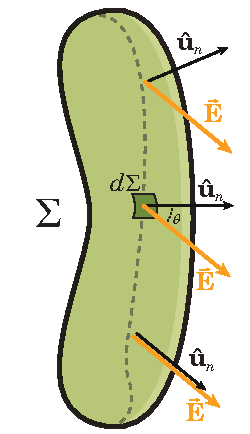
\includegraphics[width=0.75\textwidth]{images/chp2/chp2flusso.pdf}
	\end{center}
\end{minipage}
\end{define}
\begin{intuit}
	Se descriviamo la corrente di un fluido come l'acqua con un campo vettoriale $\vba{F}$, il flusso di $\vba{F}$ rappresenta \textit{quanto fluido} passa \textit{attraverso} una certa superficie per unità di tempo (anche se quest'ultima viene spesso sottintesa).\\
	Con questa interpretazione euristica si può capire anche perché l'integrale presenta nella definizione un \textit{prodotto scalare}: se l'acqua scorre perpendicolarmente alla superficie, molta acqua passerà e il flusso sarà dunque grande; al contrario, se il fluido scorre parallelamente alla superficie l'acqua non l'attraverserà mai e quindi il flusso è nullo.\\
	In altre parole, ciò che influisce sul flusso è la componente di acqua che scorre \textit{perpendicolare alla superficie}!
\end{intuit}
\noindent Come abbiamo detto, la superficie deve essere \textbf{orientabile}: detto in una maniera suggestiva, intuitiva ma non formale come piace ai fisici, deve avere due \textit{facce distinte} e due \textit{orientazioni} possibili che corrispondono alla scelta di un \textit{campo normale} che punta sempre dalla parte di una delle facce.\\
In particolare, la superficie deve essere \textit{effettivamente orientata}, ossia si deve scegliere uno dei campi normali in modo da definire quando il flusso è positivo e quando è negativo.\\
Generalmente, per convenzione si impone che il vettore normale alla superficie è orientato verso l'\textit{esterno}: quando la componente perpendicolare del campo vettoriale $\vba{E}$ e il vettore normale saranno \textit{concordi}, cioè quando $\vba{E}$ è \textit{uscente} dalla superficie, si ha un flusso \textit{positivo}; se il campo $\vba{E}$ è \textit{entrante} la superficie, allora si ha un flusso \textit{negativo}.
\begin{observe}
	~\\
	\begin{minipage}{0.34\textwidth}
		\begin{center}
			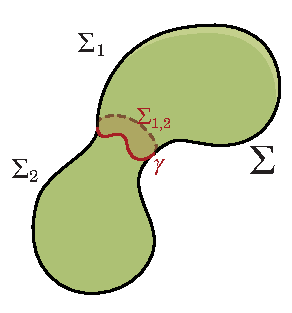
\includegraphics[width=0.95\textwidth]{images/chp2/chp2oss.pdf}
		\end{center}
	\end{minipage}	
	\begin{minipage}{0.65\textwidth}	
	Data una superficie chiusa $\Sigma$, tracciamo una curva chiusa $\gamma$ su di essa; possiamo scindere $\Sigma$ in due sottosuperfici $\Sigma_1$ e $\Sigma_2$ che hanno in comune una superficie $\Sigma_{1,2}$ delimitata da $\gamma$.
	Il flusso per linearità di scinde in
	\begin{equation*}
		\Phi_{\Sigma}=\Phi_{\Sigma_1}+\Phi_{\Sigma_2}
	\end{equation*}
	In realtà, il flusso \textit{non} è influenzato da quale sia la superficie  $\Sigma_{1,2}$: infatti, per uno dei sottoflussi il contribuito dato da $ \Sigma_{1,2}$ sarà negativo perché il campo è entrante, ma per l'altro sottoflusso sarà positivo perché il campo è uscente.
\end{minipage}
\begin{equation*}
	\Phi_{\Sigma}=\Phi_{\Sigma_1}+\Phi_{\Sigma_2}=\Phi_{\Sigma_1-\Sigma_{1,2}}+\Phi_{\Sigma_{1,2}}+\Phi_{\Sigma_2-\Sigma_{1,2}}-\Phi_{\Sigma_{1,2}}=\Phi_{\Sigma_1-\Sigma_{1,2}}+\Phi_{\Sigma_2-\Sigma_{1,2}}
\end{equation*}
\end{observe}
\section{Legge di Gauss}
\begin{theorema}[Legge di Gauss]\index{legge!di Gauss}
	Il flusso del campo elettrostatico $\vba{E}$ attraverso un superficie \textbf{chiusa} è uguale alla somma algebrica (\textrm{o nel caso di una distribuzione continua}, dell'integrale) delle cariche contenute all'\textbf{interno} della superficie, comunque siano distribuite, divisa per $\epsilon_0$.
	\begin{itemize}
		\item \textbf{Caso discreto:}
		\begin{equation}
			\tcboxmath[colback=yellowpastellow!30!white,colframe=redsalsa!85!black,drop fuzzy shadow, nobeforeafter, math upper, tcbox raise base, enhanced]{\Phi_\Sigma(\vba{E})=\frac{\left(\sum_i q_i\right)_{int}}{\epsilon_0}}\label{LeggeGaussDiscreta}
		\end{equation}
		\item \textbf{Caso continuo:}
		\begin{equation}
			\tcboxmath[colback=yellowpastellow!30!white,colframe=redsalsa!85!black,drop fuzzy shadow, nobeforeafter, math upper, tcbox raise base, enhanced]{\Phi_\Sigma(\vba{E})=\frac{1}{\epsilon_0}\int_{V}\rho\left(x,y,z\right)dV\qquad\text{tale che}\qquad \partial V=\Sigma}\label{LeggeGaussContinua}
		\end{equation}
	\end{itemize}
\end{theorema}
Lo dimostreremo per una \textit{singola} carica contenuta nella superficie - dato che il caso per molteplici cariche e per una distribuzione continua seguono immediatamente - ma prima di farlo in modo formale, vediamo una derivazione più ``fisica''.
\paragraph{Angolo solido}
Per far ciò, ci servirà la nozione di \textit{angolo solido}.
\begin{define}[Angolo solido]
	L'\textbf{angolo solido}\index{angolo solido} è una generalizzazione a tre dimensioni dell'angolo piano e misura la parte di spazio compresa entro un fascio di semirette uscenti intorno ad un punto $P$.\\
	\begin{minipage}{0.67\textwidth}
		In termini matematici, esso è definito come l'area sulla \textit{sfera unitaria} intorno a $P$ individuata dalla superficie (finita) $\Sigma$:
		\begin{equation}
		\tcboxmath[colback=yellowpastellow!30!white,colframe=ceruleancrayola!85!black,drop fuzzy shadow, nobeforeafter, math upper, tcbox raise base, enhanced]{\Omega=\int d\Omega =\int \frac{d\Sigma_0}{r^2}=\int\frac{\cos\theta d\Sigma}{r^2}}
		\end{equation}
		dove
	\end{minipage}\hspace{5pt}
	\begin{minipage}{0.32\textwidth}
		\begin{center}
			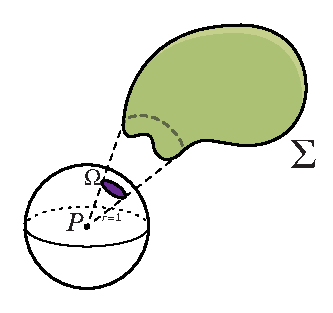
\includegraphics[width=0.9\textwidth]{images/chp2/chp2angolosolido.pdf}
		\end{center}
	\end{minipage}
\begin{itemize}
	\item $d\Omega$ è l'angolo solido infinitesimo.
	\item $d\Sigma_0$ è la \textit{proiezione ortogonale} al raggio $r$ dell'elemento infinitesimo di superficie $d\Sigma$.
	\item $\theta$ è l'\textit{angolo polare} delle coordinate sferiche.
\end{itemize}
\end{define}
Poiché $d\Sigma_0$ è un elemento infinitesimo della calotta sferica, data una parametrizzazione in coordinate sferiche vale
\begin{equation*}
	d\Sigma_0=r^2\sin\theta d\theta d\phi
\end{equation*}
da cui segue che
\begin{equation}
	d\Sigma=\sin\theta d\theta d\phi
\end{equation}
Integrando $\theta$ da $0$ a $\pi$ e $\phi$ da $0$ a $2\pi$, si ottiene l'angolo solido sotto cui dal centro $P$ è vista tutta la superficie:
\begin{equation}
	\Omega=\int d\Omega=\int_0^{2\pi}d\phi\int_0^\pi d\theta\sin\theta=4\pi
\end{equation}
Questo risultato è valido per una qualunque superficie \textit{chiusa} che racchiuda $P$ - e ne corrisponde al valore massimo dell'angolo solido.\\
\begin{units}~\\
	\textbf{\textsc{Angolo solido:}} Steradiante  ($\unit{\steradian}$).\\
	\textit{Dimensioni:} $[\Omega]=\mathsf{1}$.
\end{units}
\paragraph{Derivazione fisica della legge di Gauss}
Dato il campo di Coulomb $\vba{E}$ generato dalla carica $q$, vogliamo determinare l'elemento di flusso infinitesimo $d\Phi(\vba{E})$, ossia il flusso tramite l'elemento d'area infinitesimo $d\Sigma$.
\begin{center}
	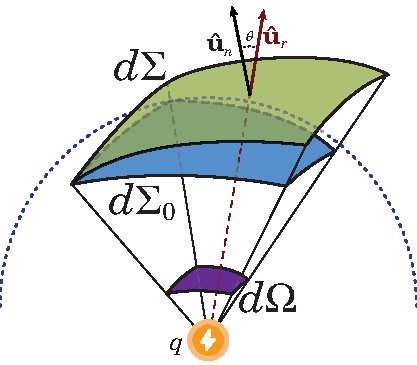
\includegraphics[width=0.36\textwidth]{images/chp2/chp2flussodim1.pdf}
\end{center}
Innanzitutto, si noti che l'angolo tra il versore radiale $\vbh{u}_r$ uscente dalla carica $q$ e il versore normale $\vbh{u}_n$ alla superficie coincide con un possibile angolo polare $\theta$ che parametrizza un punto della calotta sferica unitaria centrata in $q$.
\begin{equation*}
\vbh{u}_r\vdot\vbh{u}_n=\cos\theta
\end{equation*}
Il flusso infinitesimo diventa
\begin{equation*}
	d\Phi_{\Sigma}(\vba{E})=\vba{E}\vdot\vbh{u}_nd\Sigma=\frac{q}{4\pi\epsilon_0}\frac{\vbh{u}_r\vdot\vbh{u}_n}{r^2}d\Sigma=\frac{q}{4\pi\epsilon_0}\frac{\cos\theta}{r^2}d\Sigma=\frac{q}{4\pi\epsilon_0}\frac{d\Sigma_0}{r^2}=\frac{q}{4\pi\epsilon_0}d\Omega
\end{equation*}
\begin{observe}
	Il flusso del campo $\vba{E}$ generato da una carica puntiforme dipende solo dall'angolo solido e \textit{non} dalla superficie o dalla distanza dalla carica: il flusso è lo stesso per qualunque superficie il cui bordo si appoggi sul cono individuato dall'angolo solido.\\
	Questo è una \textit{diretta} conseguenza che il campo di Coulomb presenta un fattore $\nicefrac{1}{r^2}$; se la relazione fosse stata anche solo leggermente diversa non varrebbe tale dipendenza.
\end{observe}
Per una superficie (finita) e chiusa che racchiude la carica $q$ si ha
 \begin{equation*}
 	\Phi_\Sigma(\vba{E})=\frac{q}{4\pi\epsilon_0}\Omega=\frac{q}{\epsilon_0}
 \end{equation*}
\paragraph{Dimostrazione formale della legge di Gauss}
\begin{demonstration}
	Consideriamo inizialmente il caso con una carica sola. Per semplicità, poniamo l'origine del nostro sistema di riferimento dove è situata la carica. Data la simmetria di carattere radiale fornita dal campo elettrostatico di Coulomb, ci conviene utilizzare le coordinate sferiche
	\begin{equation*}
		\begin{cases}
			x=r\sin\theta\cos\phi\\
			y=r\sin\theta\sin\phi\\
			z=r\cos\theta
		\end{cases}
	\end{equation*}
	Parametrizziamo la superficie $\Sigma$ con l'angolo \textit{polare} $\theta$ e l'angolo \textit{azimutale} $\phi$ delle coordinate sferiche:
	\begin{align*}
		\vba{r}(\theta,\phi)&=x(\theta,\phi)\vba{u}_x+y(\theta,\phi)\vba{u}_y+z(\theta,\phi)\vba{u}_z=\\
		&=r(\theta,\phi)\sin\theta\cos\phi\vba{u}_x+r(\theta,\phi)\sin\theta\sin\phi\vba{u}_y+r(\theta,\phi)\cos\theta\vba{u}_z
	\end{align*}
	Osserviamo che per descrivere una superficie con le coordinate sferiche è necessario fornire la \textit{distanza} $r(\theta,\phi)$ dall'origine nella direzione indicata dagli angoli $\theta$ e $\phi$. Anzi, la parametrizzazione può essere espressa totalmente in termini \textit{radiali}! Infatti, il versore radiale è dato da
	\begin{equation*}
		\vbh{u}_r=\frac{\vbh{e}_r}{\abs{\vbh{e}_r}}=\frac{\pdv{x^i}{r}\vbh{u}_i}{1}=\sin\theta\cos\phi\vbh{u}_x+\sin\theta\sin\phi\vbh{u}_y+\cos\theta\vbh{u}_z
	\end{equation*}
	Raccogliendo $r(\theta,\phi)$ dalla parametrizzazione scritta prima si ottiene quindi
	\begin{equation*}
		\vba{r}(\theta,\phi)=r(\theta,\phi)\vbh{u}_r
	\end{equation*}
	Per definizione, il flusso è
	\begin{equation*}
		\Phi_{\Sigma}(\vba{E})=\int_{\Sigma}\vba{E}\vdot\vbh{u}_nd\Sigma=\int_{\Sigma}\vba{E}\vdot\vbh{u}_n\abs{\pdv{\vba{r}(\theta,\phi)}{\theta}\cross\pdv{\vba{r}(\theta,\phi)}{\phi}}d\theta d\phi\squarequal
	\end{equation*}
	Poiché il versore normale è
	\begin{equation*}
		\vbh{u}_n=\frac{\pdv{\vba{r}(\theta,\phi)}{\theta}\cross\pdv{\vba{r}(\theta,\phi)}{\phi}}{\abs{\pdv{\vba{r}(\theta,\phi)}{\theta}\cross\pdv{\vba{r}(\theta,\phi)}{\phi}}}
	\end{equation*}
	il flusso si può calcolare come
	\begin{equation*}
		\squarequal\int_{\Sigma}\vba{E}\vdot\pdv{\vba{r}(\theta,\phi)}{\theta}\cross\pdv{\vba{r}(\theta,\phi)}{\phi} d\theta d\phi=\frac{q}{4\pi\epsilon_0}\int_{\Sigma}\frac{1}{r(\theta,\phi)^2}\vbh{u}_r\vdot \pdv{\vba{r}(\theta,\phi)}{\theta}\cross\pdv{\vba{r}(\theta,\phi)}{\phi} d\theta d\phi
	\end{equation*}
	Per semplificare quel prodotto misto, dobbiamo prima analizzare i termini che partecipano al prodotto vettoriale.\\
	In un generico punto\footnote{Qui indicato tramite le coordinate ad esso associate dalla parametrizzazione.} $\left(\theta,\phi\right)$ della superficie, i vettori della base del piano tangente alla superficie in tal punto sono
	\begin{equation*}
		\begin{cases}
			\pdv{\vba{r}}{\theta}=\pdv{\theta}\left(r(\theta,\phi)\vba{u}_r\right)=\pdv{r(\theta,\phi)}{\theta}\vbh{u}_r+r(\theta,\phi)\pdv{\vbh{u}_r}{\theta}\\
			\pdv{\vba{r}}{\phi}=\pdv{\phi}\left(r(\theta,\phi)\vba{u}_r\right)=\pdv{r(\theta,\phi)}{\phi}\vbh{u}_r+r(\theta,\phi)\pdv{\vbh{u}_r}{\phi}\\
		\end{cases}
	\end{equation*}
	Si nota subito che  le componenti parallele a $\vba{u}_r$ \textit{non} influiscono al flusso. Al netto di costanti moltiplicative, il contribuito di tali componenti è un $\vba{u}_r$ nel prodotto vettoriale del prodotto misto, ma valendo
\begin{equation*}
	\begin{cases}
		\vbh{u}_r\vdot\vbh{u}_r\cross\vba{a}=0\\
		\vbh{u}_r\vdot\vba{a}\cross\vbh{u}_r=0
	\end{cases}\forall \vba{a}\text{ vettore}
\end{equation*}
tali componenti non cambieranno in alcun modo il flusso; ciò che invece lo cambia sono le derivate dei versori radiali. Sviluppando, l'espressione del flusso si ha
\begin{align*}
	\Phi_{\Sigma}(\vba{E})&=\frac{q}{4\pi\epsilon_0}\int_{\Sigma}\frac{1}{r(\theta,\phi)}\vbh{u}_r\vdot \pdv{\vba{r}(\theta,\phi)}{\theta}\cross\pdv{\vba{r}(\theta,\phi)}{\phi} d\theta d\phi=\\
	&=\frac{q}{4\pi\epsilon_0}\int_{\Sigma}\frac{1}{\Ccancel[red]{r(\theta,\phi)^2}}\vbh{u}_r\vdot\left(\Ccancel[red]{r(\theta,\phi)}\pdv{\vbh{u}_r}{\theta}\cross \Ccancel[red]{r(\theta,\phi)}\pdv{\vbh{u}_r}{\phi}\right)d\theta d\phi=\\
	&=\frac{q}{4\pi\epsilon_0}\int_{\Sigma}\vbh{u}_r\vdot\pdv{\vbh{u}_r}{\theta}\cross\pdv{\vbh{u}_r}{\phi}d\theta d\phi
\end{align*}
Poiché
\begin{equation*}
	\begin{cases}
		\pdv{\vbh{u}_r}{\theta}=\cos\theta\cos\phi\vbh{u}_x+\cos\theta\sin\phi\vbh{u}_y-\sin\theta\vbh{u}_z\\
		\pdv{\vbh{u}_r}{\phi}=-\sin\theta\sin\phi\vbh{u}_x+\sin\theta\cos\phi\vbh{u}_y\\
\end{cases}
\end{equation*}
e
\begin{equation*}
	\vbh{u}_r\vdot\pdv{\vbh{u}_r}{\theta}\cross\pdv{\vbh{u}_r}{\phi}=\begin{vmatrix}
		\sin\theta\cos\phi & \sin\theta\sin\phi & \cos\theta\\
		\cos\theta\cos\phi & \cos\theta\sin\phi & -\sin\theta\\
		-\sin\theta\sin\phi & \sin\theta\cos\phi & 0
	\end{vmatrix}=\sin\theta
\end{equation*}
segue che
\begin{equation}
	\Phi_{\Sigma}(\vba{E})=\frac{q}{4\pi\epsilon_0}\int_{\Sigma}\sin\theta d\theta d\phi=\frac{q}{4\pi\epsilon_0}\Omega\label{LeggeGaussGeneralizzata}
\end{equation}
dove $\Sigma$ è l'angolo solido sull'intera superficie.\\
Se la superficie (finita) è chiusa si ha $\Omega=4\pi$, ottenendo quindi il risultato desiderato.\\
Il caso per cariche multiple segue dal \textit{principio di sovrapposizione} dei campi elettrici:
\begin{equation*}
	\Phi_{\Sigma}(\vba{E})=\int_{\Sigma} \vba{E}\vdot \vbh{u}_nd\Sigma=\int_{\Sigma}\left(\sum_i\vba{E}_i\right)\vdot\vbh{u}_nd\Sigma=\sum_i\int_{\Sigma}\vba{E}_i\vdot\vbh{u}_nd\Sigma=\sum_i\frac{q_i}{\epsilon_0}
\end{equation*}
Da questa si ottiene, passando al continuo, la relazione \eqref{LeggeGaussContinua}.
\end{demonstration}
\begin{observe}
	La \eqref{LeggeGaussGeneralizzata} descrive il flusso del campo elettrostatico attraverso una superficie \textbf{qualunque}. La legge di Gauss si potrebbe vedere come un \textit{caso specifico} di questa relazione.
\end{observe}
\begin{digression}\label{LeggeGaussMoltoGeneralizzata}
	La dimostrazione della legge di Gauss si basa sul fatto fondamentale che la legge di Coulomb, che descrive l'interazione tra cariche elettriche, è \textit{inversamente proporzionale} a $r^2$. È dunque possibile adattare la legge di Gauss in altri contesti non elettrici, se consideriamo una forza tra due enti inversamente proporzionale a $r^2$.\\
	Ad esempio, esiste una formulazione della legge di Gauss per la \textit{forza di gravitazione} completamente equivalente alla legge di gravitazione universale di Newton: il flusso del campo gravitazionale attraverso una superficie chiusa è pari alla massa inclusa in essa, moltiplicata per $-4\pi G$.
	\begin{itemize}
		\item \textbf{Caso discreto:}
		\begin{equation}
			\Phi_\Sigma(\vba{G})=-4\pi G\sum_i m_i
		\end{equation}
		\item \textbf{Caso continuo:}
		\begin{equation}
			\Phi_\Sigma(\vba{G})=-4\pi G\int_{V}\rho\left(x,y,z\right)dV\qquad\text{tale che}\ \partial V=\Sigma
		\end{equation}
	\end{itemize}
	Si noti, tra l'altro, che non è particolarmente differente dal caso elettrico dato che la legge di Gauss per il campo elettrico si può anche scrivere così:
	\begin{itemize}
		\item \textbf{Caso discreto:}
		\begin{equation*}
			\Phi_\Sigma(\vba{E})=4\pi k\sum_i q_i
		\end{equation*}
		\item \textbf{Caso continuo:}
		\begin{equation}
			\Phi_\Sigma(\vba{E})=4\pi k\int_{V}\rho\left(x,y,z\right)dV\qquad\text{tale che}\ \partial V=\Sigma
		\end{equation}
	\end{itemize}
\end{digression}
\paragraph{Flusso tramite una superficie chiusa per una carica esterna}
La legge di Gauss descrive il flusso tramite una superficie chiusa tenendo conto delle cariche \textit{interne} ad essa... e si ci fossero delle cariche \textit{esterne}?

Limitiamoci all'inizio al caso di una singola carica esterna: il campo di Coulomb entra nella superficie chiusa, attraversa lo spazio contenuto da essa e poi esce dall'altro lato. In termini di angolo solido, il cono elementare che sottende l'angolo solido infinitesimo $d\Sigma$ determina sulla superficie chiusa due elementi $d\Sigma_1$ e $d\Sigma_2$. Per la convenzione sul segno del flusso:
\begin{itemize}
	\item $\vba{E}$ \textit{entra} in $d\Sigma_1$: $\vba{E}\vdot \vbh{u}_n d\Sigma_1<0$.
	\item $\vba{E}$ \textit{esce} da $d\Sigma_2$: $\vba{E}\vdot \vbh{u}_n d\Sigma_2>0$.
\end{itemize}
I flussi infinitesimi che otteniamo\footnote{Il procedimento è analogo a quello con cui si ottiene l'equazione \eqref{LeggeGaussGeneralizzata}.} sono
\begin{equation*}
	\begin{cases}
		d\Phi_{\Sigma_1}(\vba{E})=\vba{E}\vdot \vbh{u}_n d\Sigma_1=-\frac{q}{4\pi\epsilon_0}d\Omega\\
		d\Phi_{\Sigma_2}(\vba{E})=\vba{E}\vdot \vbh{u}_n d\Sigma_2=\frac{q}{4\pi\epsilon_0}d\Omega
	\end{cases}
\end{equation*}
Integrando sull'intera superficie chiusa otteniamo
\begin{equation}
	\Phi_\Sigma(\vba{E})=\int_{\Sigma}\vba{E}\vdot\vbh{u}_nd\Sigma=0
\end{equation}
Il flusso tramite una superficie \textit{chiusa} dipende \textit{solo} dalle cariche interne ad essa.
\begin{observe}
	Cosa cambia dal caso della carica interna? Il campo elettrico in quella situazione risulta essere \textit{entrante} (se la carica è positiva) o \textit{uscente} (se la carica è negativa) da ogni elemento infinitesimo; il flusso avrà quindi sempre lo stesso segno oppure essere nullo, ma sulla superficie intera questo si ha solo se questa è parallela al campo.   
\end{observe}
\section{Applicazioni della legge di Gauss}
La legge di Gauss, in linea di principio, ci descrive solo il flusso tramite una superficie chiusa. Tuttavia, in situazioni di \textit{evidenti simmetrie}, confrontando la definizione di flusso con quello ottenuto dalla legge di Gauss possiamo sorprendentemente calcolare in modo abbastanza facile il campo elettrostatico che genera il flusso.
\begin{attention}
	Bisogna fare attenzione ad utilizzare la legge di Gauss in \textit{assenza di simmetrie}. Ad esempio, consideriamo una situazione come in figura.
	\begin{center}
		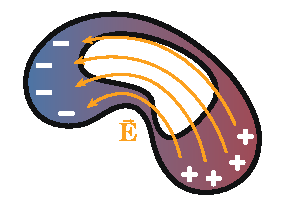
\includegraphics[width=0.4\textwidth]{images/chp2/chp2gaussnosimm.pdf}
	\end{center}
	Qui il flusso attraverso la superficie interna è nullo perché ciò che entra esce, ma il campo elettrico \textit{non} è nullo!
\end{attention}
\paragraph{Filo carico rettilineo (infinito)}
	Si consideri un filo rettilineo infinito con densità lineare costante $\lambda$. Per semplicità, poniamo il sistema di riferimento in modo che il filo carico sia lungo l'asse $z$. Poniamo un cilindro attorno al filo in modo che il filo passi per l'asse del cilindro.\\
	\begin{minipage}{0.29\textwidth}
		\begin{center}
			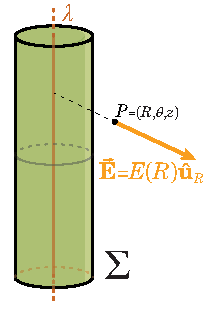
\includegraphics[width=1\textwidth]{images/chp2/chp2filoinfinito.pdf}
		\end{center}
	\end{minipage}\hspace{10pt}
	\begin{minipage}{0.7\textwidth}
		Data l'evidente simmetria cilindrica del sistema usiamo, per motivi che dovrebbero essere oramai chiari, le coordinate cilindriche:
		\begin{equation*}
			\begin{cases}
				x=R\cos\theta\\
				y=R\sin\theta\\
				z=z
			\end{cases}
		\end{equation*}
		Oltre ad essere un sistema di riferimento, fissato $R$ abbiamo una parametrizzazione del cilindro di raggio $R$. Ora, ci è già noto che in questo sistema di riferimento il campo elettrostatico dipende esclusivamente dalla \textit{coordinata radiale} e ha direzione radiale, ossia $\vba{E}=E(R)\vbh{u}_R$.
	\end{minipage}\\
Per come abbiamo posto il cilindro $\Sigma$, il versore normale alla superficie laterale coincide con quello radiale delle coordinate cilindriche, pertanto
\begin{equation*}
	\Phi_{\Sigma}(\vba{E})=\int_{\Sigma}\vba{E}\cdot\vbh{u}_nd\Sigma=\int_{\Sigma}\vba{E}\cdot\vbh{u}_Rd\Sigma=\int_{\Sigma} E(R)\vbh{u}_R\vdot\vbh{u}_Rd\Sigma=E(R)\int_{\Sigma} d\Sigma\squarequal
\end{equation*}
dove l'ultimo passaggio è lecito in quanto sulla superficie del cilindro il raggio è fissato e quindi anche $E(R)$ è costante.\\
Dato che l'elemento di area è dato da $d\Sigma=d\Phi dz$, si ha
\begin{equation*}
	\squarequal\lim_{L\to+\infty}2\pi R L E(R)
\end{equation*}
Per la legge di Gauss,
\begin{equation*}
	\Phi_{\Sigma}(\vba{E})=\frac{q}{\epsilon_0}=\frac{\lambda L}{\epsilon_0}
\end{equation*}
dove $\lambda$ è la densità lineare di carica; per ottenere il flusso per il filo infinito ci basterebbe mandare $L$ all'infinito. Eguagliando i due flussi ottenuti si ricava che
\begin{equation*}
	2\pi R\Ccancel[red]{L}E(R)=\frac{\lambda \Ccancel[red]{L}}{\epsilon_0}
\end{equation*}
e quindi
\begin{equation}
	\tcboxmath[colback=yellowpastellow!30!white,drop fuzzy shadow, nobeforeafter, math upper, tcbox raise base, enhanced]{\vba{E}(R)=\frac{\lambda}{2\pi\epsilon_0 R}}
\end{equation}
\paragraph{Superficie piana carica infinita}\label{pianocarico}
Si consideri una superficie piana $\Sigma$ con densità superficiale costante $\sigma$. Per semplicità, poniamo il sistema di riferimento in modo che la superficie coincida con il piano $x=0$. Come per il caso del filo carico rettilineo, consideriamo un cilindro, questa volta che interseca la superficie ortogonalmente e posto in maniera che le basi siano alla stessa distanza dal piano.\\
\begin{minipage}{0.43\textwidth}
	\begin{center}
		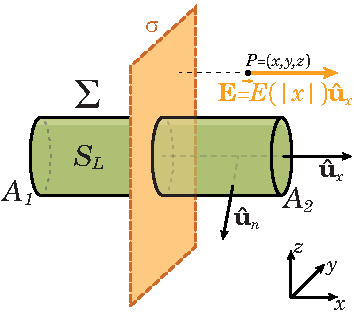
\includegraphics[width=1\textwidth]{images/chp2/chp2superficieinfinita.pdf}
	\end{center}
\end{minipage}\hspace{10pt}
\begin{minipage}{0.56\textwidth}
	Ci è già noto che il campo elettrostatico dipende esclusivamente dalla coordinata perpendicolare al piano, cioè $x$, e ha direzione $\vbh{u}_x$. In particolare, si osservi che da facce opposte del piano il versore normale $u_n=u_x$ cambia verso e quindi cambia verso anche il campo elettrostatico:
	\begin{equation*}
		\vba{E}=
		\begin{cases}
			E(\abs{x})\vbh{u}_x&\text{se}\ x>0\\
			-E(\abs{x})\vbh{u}_x&\text{se}\ x<0
		\end{cases}
	\end{equation*}
	Il flusso tramite il cilindro $\Sigma$ si può scindere in tre componenti: i due flussi $\Phi_{A_1}$ e $\Phi_{A_2}$ attraverso le basi e il flusso $\Phi_{SL}$ attraverso la superficie laterale.
\end{minipage}\\
Tuttavia, poiché la superficie laterale è sempre ortogonale al campo, quest'ultima componente è nulla; inoltre, si ha che il campi esce sempre dalle basi, pertanto i flussi saranno positivi e, per questioni di simmetria, coincidono:
\begin{equation*}
	\Phi_{A_1}=\Phi_{A_2}
\end{equation*}
Pertanto,
\begin{equation*}
	\Phi_{\Sigma}(\vba{E})=2\int_A E(\abs{x})d\Sigma=2 E(\abs{x})\int_{A_1}d\Sigma=2E(\abs{x})A_1
\end{equation*}
Ricordando che la densità di carica superficiale $\sigma$ è costante, la carica interna al cilindro è data da
\begin{equation*}
	q=\sigma A_1
\end{equation*}
Per la legge di Gauss si ha
\begin{equation*}
	\Phi_{\Sigma}=\frac{\sigma A_1}{\epsilon_0}
\end{equation*}
Eguagliando i due flussi ottenuti si ricava che
\begin{equation*}
	2\Ccancel[red]{A_1}E(\abs{x})=\frac{\sigma \Ccancel[red]{A_1}}{\epsilon_0}
\end{equation*}
e quindi
\begin{equation}
	\tcboxmath[colback=yellowpastellow!30!white,drop fuzzy shadow, nobeforeafter, math upper, tcbox raise base, enhanced]{\vba{E}(\abs{x})=\frac{\sigma}{2\epsilon_0}\vbh{u}_x}
\end{equation}
\paragraph{Sfera uniformemente carica}
Si consideri una palla sferica di raggio $R$ con densità volumica costante $\rho$. Per semplicità, poniamo il sistema di riferimento in modo che l'origine coincida con il centro della sfera. Come superficie $\Sigma$ per calcolare il flusso scelgo una sfera di raggio $r$ centrata anch'essa nell'origine.
Ci è già noto che il campo elettrostatico dipende esclusivamente dalla coordinata radiale e ha direzione radiale, ossia $\vba{E}=E(r)\vbh{u}_r$. Il versore normale alla superficie $\Sigma$ è $\vbh{u}_n=\vbh{u}_r$.
A questo punto distinguiamo il calcolo quando la superficie sferica ha raggio maggiore della palla ($r>R$) o quando ha raggio minore ($r<R$).
\begin{itemize}
	\item \textbf{Il caso esterno:} $r>R$.\\
	\begin{minipage}{0.4\textwidth}
		\begin{center}
			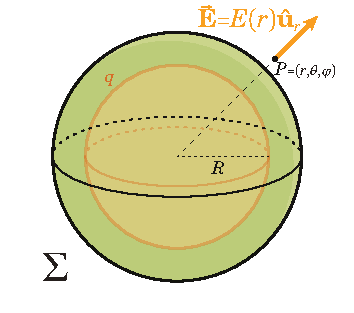
\includegraphics[width=1\textwidth]{images/chp2/chp2sferacarica1.pdf}
		\end{center}
	\end{minipage}
	\begin{minipage}{0.5\textwidth}
		In questo caso la superficie sferica \textit{contiene} la sfera uniformemente carica. Il flusso dunque è
		\begin{equation*}
			\Phi_{\Sigma}(\vba{E})=\int E(r)d\Sigma=E(r)4\pi r^2
		\end{equation*}
		dato che $E(r)$ è costante sulla sfera di raggio $r$.
		La superficie sferica contiene \textit{tutta} la carica della palla al suo interno, quindi per la legge di Gauss
		\begin{equation*}
			\Phi_{\Sigma}(\vba{E})=\frac{q}{\epsilon_0}=\frac{4 \pi R^3\rho}{3\epsilon_0}
		\end{equation*}
		e quindi
		\begin{equation}
			\vba{E}(r)=\frac{\rho R^3}{3\epsilon_0r^2}\vbh{u}_r=\frac{q}{4\pi\epsilon_0 r^2}\vbh{u}_r
		\end{equation}
	\end{minipage}\\
\end{itemize}
\begin{observe}
	Una qualunque distribuzione di carica a simmetria \textit{sferica} dipendente dalla distanza radiale, ossia $\rho(x,y,z)=\rho(r)$, genera al suo esterno un campo uguale a quello di una carica puntiforme.
\end{observe}
\begin{itemize}
	\item \textbf{Il caso interno:} $r<R$\\
	\begin{minipage}{0.4\textwidth}
		\begin{center}
			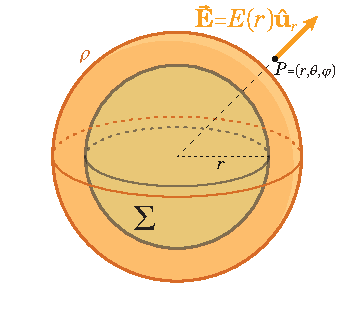
\includegraphics[width=1\textwidth]{images/chp2/chp2sferacarica2.pdf}
		\end{center}
	\end{minipage}
	\begin{minipage}{0.5\textwidth}
		In questo caso la superficie sferica contiene al suo interno solo \textit{una parte} della carica complessiva:
		\begin{equation*}
			q_{int}=\frac{4}{3}\pi r^3\rho
		\end{equation*}
		Se il flusso, calcolato secondo la definizione, non cambia espressione (ma valore sì!)...
		\begin{equation*}
			\Phi_{\Sigma}(\vba{E})=E(r)4\pi r^2
		\end{equation*}
		... quello per la legge di Gauss diventa
		\begin{equation*}
			\Phi_{\Sigma}(\vba{E})=\frac{q_{int}}{\epsilon_0}=\frac{4 \pi r^3\rho}{3\epsilon_0}
		\end{equation*}
		e quindi
		\begin{equation}
			\vba{E}(r)=\frac{q_{int}}{4\pi\epsilon_0 r^2}\vbh{u}_r=\frac{\rho r}{3\epsilon_0}\vbh{u}_r
		\end{equation}
	\end{minipage}
\end{itemize}
Riassumendo, il campo elettrico generato da una sfera uniformemente carica di raggio $R$ a distanza $r$ dall'origine è
\begin{equation}
	\tcboxmath[colback=yellowpastellow!30!white,drop fuzzy shadow, nobeforeafter, math upper, tcbox raise base, enhanced]{\vba{E}(r)=\begin{cases}
		\displaystyle\frac{\rho r}{3\epsilon_0}\vbh{u}_r&\text{se}\ r< R\\
		\displaystyle\frac{q}{4\pi\epsilon_0 r^2}\vbh{u}_r=\frac{\rho R^3}{3\epsilon_0r^2}\vbh{u}_r &\text{se}\ r> R
	\end{cases}}
\end{equation}
\begin{center}
	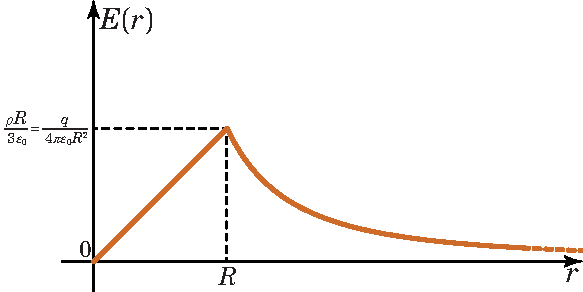
\includegraphics[width=0.75\textwidth]{images/chp2/chp2sferagraf1.pdf}
\end{center}
Come già detto, esiste un \textit{potenziale} $V$ tale per cui $\vba{E}=-\grad{V}$. Poiché il campo dipende esclusivamente dalla coordinata radiale, tale relazione si trasforma in
\begin{equation*}
	E(r)=-\pdv{V}{r}
\end{equation*}
da cui
\begin{equation*}
	V(r)=-\int E(r)dr+A
\end{equation*}
dove $A$ è una costante che dipende dalle \textit{condizioni al contorno} di natura fisica. Lasciando tempo alle opportune spiegazioni, per ora ci basti sapere che il \textit{limite all'infinito} del potenziale si pone in generale \textit{nullo}\footnote{Nel \autoref{chap:PotenzialeElettrico}, a pag. \pageref{CondizionialContornoPot} si può trovare la motivazione di ciò.} e che il potenziale è un campo scalare \textit{continuo}\footnote{Nel \autoref{chap:PotenzialeElettrico}, a pag. \pageref{PotenzialeContinuo} si può trovare la motivazione di ciò.}. Integrando le equazioni di campo ottenute ricaviamo
\begin{equation*}
	V(r)=\begin{cases}
		\displaystyle-\frac{\rho r^2}{6\epsilon_0} + A&\text{se}\ r< R\\
		\displaystyle\frac{q}{4\pi\epsilon_0 r} + B=\frac{\rho R^3}{3\epsilon_0r} + B&\text{se}\ r> R
	\end{cases}
\end{equation*}
con $A$ e $B$ opportune costanti. Imponiamo nella seconda equazione il potenziale all'infinito ($r\to+\infty$) nullo - dato che è quella riguardante il sistema a grandi distanze; è immediato trovare che $B=0$. Dalla condizione di continuità invece, il potenziale sul bordo della sfera deve essere uguale ``visto'' dall'\textit{interno} e dall'\textit{esterno}, ossia
\begin{equation*}
	\frac{\rho R^3}{3\epsilon_0R}=-\frac{\rho R^2}{6\epsilon_0} + A
\end{equation*}
Con pochi passi algebrici troviamo
\begin{equation*}
	A=\frac{\rho R^2}{2\epsilon_0}
\end{equation*}
Riassumendo, il potenziale del campo elettrico generato da una sfera uniformemente carica di raggio $R$ a distanza $r$ dall'origine è
\begin{equation}
	\tcboxmath[colback=yellowpastellow!30!white,drop fuzzy shadow, nobeforeafter, math upper, tcbox raise base, enhanced]{V(r)=\begin{cases}
		\displaystyle-\frac{\rho r^2}{6\epsilon_0} + \frac{\rho R^2}{2\epsilon_0}&\text{se}\ r< R\\
		\displaystyle\frac{q}{4\pi\epsilon_0 r} + B=\frac{\rho R^3}{3\epsilon_0r} + B&\text{se}\ r> R
	\end{cases}}
\end{equation}
\begin{center}
	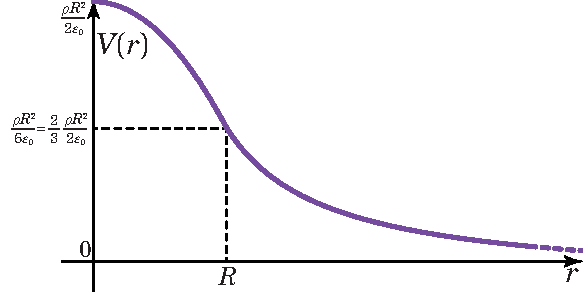
\includegraphics[width=0.75\textwidth]{images/chp2/chp2sferagraf2.pdf}
\end{center}
\begin{observe}
	Poiché il sistema ha una dimensione radiale \textit{finita}, si ha come conseguenza la \textit{diminuzione continua} del campo fino all'\textit{annullamento nel campo} nel centro della distribuzione: in questo modo si evita la divergenza all'infinito che si ha con il campo della \textit{carica puntiforme}, oggetto che \textit{fisicamente} è \textit{irrealizzabile} nella teoria classica dell'elettromagnetismo.
\end{observe}
\section{Equilibrio in un campo elettrostatico}
\begin{define}[Equilibrio stabile]
	Un punto $P$ è di \textbf{equilibrio stabile}\index{equilibrio!stabile} per un corpo puntiforme se per un qualsiasi spostamento, piccolo a piacere, da tale posizione esistono forze che riportano l'oggetto nella posizione originale.
\end{define}
\begin{define}[Equilibrio instabile]
	Un punto $P$ è di \textbf{equilibrio instabile}\index{equilibrio!instabile} per un corpo puntiforme se esistono spostamenti, piccolo a piacere, da tale posizione esistono forze che riportano l'oggetto nella posizione originale.
\end{define}
Consideriamo delle \textit{sorgenti} fisse (continue o discrete che siano, \textit{non} cambia) nel vuoto e sia $\vba{E}(\vba{r})$ il campo elettrico generato da queste cariche. Esistono dei punti tali per cui, se poniamo una carica $q$ lì, essa rimarrà in equilibrio stabile?\\
La risposta è \textbf{no} e ce lo dice il \textbf{teorema di Earnshaw}.
\begin{theorema}[Teorema di Earnshaw]\index{teorema!di Earnshaw}
	Una collezione di cariche puntuali non possono essere mantenute in una configurazione di equilibrio stabile soltanto dall'interazione elettrostatica delle cariche con un campo elettrico.
\end{theorema}
In questa dimostrazione assumiamo che la carica sia positiva ($q>0$), ma la dimostrazione è \textit{mutatis mutandis} la stessa per $q<0$.
\begin{observe}
	La carica nella dimostrazione si suppone essere una \textbf{carica di prova}, e quindi il campo generato dalla carica $q$ è trascurabile.
\end{observe}
\begin{demonstration}
	Supponiamo che la carica, immersa nel campo elettrico e non soggetta ad altre forze, è in equilibrio stabile in $P=\vba{r}$; ciò significa che:
	\begin{enumerate}
		\item La carica di per sé è ferma; la forza totale agente sulla carica è dunque nulla, e dato che le uniche forze sulla carica in $\vba{r}$ sono le forza di Coulombsi ha
		\begin{equation*}
			\vba{F}(\vba{r})=q\vba{E}(\vba{r})=0\underset{q\neq 0}{\implies}\vba{E}(\vba{r})=0
		\end{equation*}
		\item Per un (piccolo) spostamento $\delta \vba{r}$ attorno a $\vba{r}$, la forza riporta la carica verso il punto $\vba{r}$, cioè la forza
		\begin{equation*}
			\vba{F}(\vba{r}+\delta\vba{r})=q\vba{E}(\vba{r}+\delta\vba{r})
		\end{equation*}
		deve puntare verso $\vba{r}$.\\
		\begin{minipage}{0.35\textwidth}
			\begin{center}
				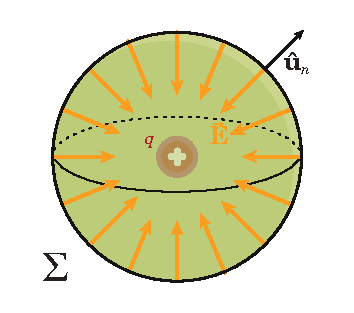
\includegraphics[width=1\textwidth]{images/chp2/chp2earnshaw.pdf}
			\end{center}
		\end{minipage}\hspace{5pt}
		\begin{minipage}{0.54\textwidth}
			Consideriamo una superficie chiusa (arbitrariamente piccola) attorno alla carica.
			Per quanto abbiamo detto, in un qualunque suo punto la forza di Coulomb in tal punto deve essere diretta verso $P=\vba{r}$. Pertanto, se il campo è entrante la superficie, il flusso tramite la superficie è negativo...
			\begin{equation}
				\Phi{\Sigma}(\vba{E})<0
			\end{equation}
		\end{minipage}\\
		... ma possiamo applicare la legge di Gauss per ricavare il valore del flusso tramite tale superficie, tuttavia si avrebbe
		\begin{equation*}
			\Phi{\Sigma}(\vba{E})=\frac{q}{\epsilon_0}<0\implies q<0
		\end{equation*}
		il che è un assurdo! Segue che non ci può essere equilibrio elettrostatico stabile.\qedhere
	\end{enumerate}
\end{demonstration}
L'unica possibilità di avere una carica in equilibrio stabile è se si trovasse esattamente nello stesso punto di un'altra carica $Q$ di segno opposto e quantità di carica maggiore. Infatti, in tal caso qualunque superficie, piccolo a piacere, scegliamo attorno al punto di equilibrio si avrà sempre flusso pari a
\begin{equation*}
	\Phi_{\Sigma}(\vba{E})=\frac{q+Q}{\epsilon_0}
\end{equation*}
per la legge di Gauss; questa volta non si ha alcun assurdo, dato che il campo elettrico è entrante e quindi il flusso è negativo e, se $\abs{Q}>\abs{q}$, allora anche il flusso secondo Gauss è negativo.
\begin{digression}
	Da quanto detto, un sistema di cariche libere \textit{dello stesso segno} non potrà ai restare in equilibrio stabile spontaneamente, ma necessariamente occorrono altre forze per vincolare le cariche.
	
	Una conseguenza di ciò è che il modello dell'atomo di Rutherford \textit{non} è stabile, essendo basato su una distribuzione fissata di cariche: nel \textit{nucleo atomico} non ci potrebbe essere più di un protone senza compromettere la stabilità del nucleo! È grazie all'interazione \textit{nucleare forte} che, essendo particolarmente forte a distanze microscopiche, i protoni superano la repulsione elettrostatica tra di loro e permettono la stabilità dell'atomo.
\end{digression}
% SVN info for this file
% SVN info for this file
\svnidlong
{$HeadURL$}
{$LastChangedDate$}
{$LastChangedRevision$}
{$LastChangedBy$}

\chapter{Il potenziale elettrico} % TO DO: Il lavoro elettrico?
\labelChapter{PotenzialeElettrico}
% TO DO: quando parlo del potenziale e del campo elettrico a tratti, sostituire il geq o leq con < e > 
\begin{introduction}
	‘‘BEEP BOOP''
	\begin{flushright}
		\textsc{Lollo BiancoBOT}, dopo aver finito le citazioni. % TO DO: quote 
	\end{flushright}
\end{introduction}
\lettrine[findent=1pt, nindent=0pt]{P}{er}  % TO DO: intro
\section{Circuitazione di un campo vettoriale}
% TO DO: concezione intuitiva di circuitazione
\begin{define}[Circuitazione di un campo vettoriale]
	Il \textbf{circuitazione di un campo vettoriale lungo una curva chiusa}\index{circuitazione di un campo vettoriale} $\gamma$, parametrizzata da una funzione $\funz[\vba{r}]{\left[a,b\right]}{\realset^3}$, è
	\begin{equation}
		\Gamma_{\gamma}\left(\vba{E}\right)=\oint_{\gamma}\vba{E}\vdot d\vba{s}=\int_{a}^b\vba{E}\vdot\frac{d\vba{r}}{dt}dt
	\end{equation}
\end{define}
\section{Forze conservative e campi vettoriali conservativi}
\paragraph{Dalle forze conservative...}
La circuitazione ha particolare rilevanza in ambito fisico; la sua prima applicazione che vedremo è in una caratterizzazione dei\textit{campi vettoriali conservativi}. Prima però, riguardiamo rapidamente il concetto di lavoro e del suo ruolo per quelle forze dette forze conservatrici, trattato nel corso di \textsc{Fisica I}.
\begin{define}[Lavoro]
	Dati due punti $\vba{r}_A$ e $\vba{r}_B$, il \textbf{lavoro}\index{lavoro} di una forza $\vba{F}$ lungo una curva $\gamma$ tra i due punti è definito come
	\begin{equation}
		W_{\gamma_1}=\int_{\gamma_1}\vba{F}\vdot d\vba{s}
	\end{equation}
\end{define}
In generale, il lavoro dipende dal \textit{percorso effettuato}: il lavoro compiuto da una stessa forza lungo due curve $\gamma_1$ e $\gamma_2$  è differente. Per un caso particolare di forze, tuttavia, il lavoro dipende esclusivamente dagli estremi e non dal percorso effettuato.
\begin{define}[Forza conservativa]
	Una forza $\vba{F}$ è detta \textbf{conservativa}\index{forza!conservativa} se per qualunque curva $\gamma_1,\ \gamma_2$ tra due punti $\vba{r}_A$ e $\vba{r}_B$ il lavoro è
	\begin{equation}
		W_{\gamma_1}=W_{\gamma_2}
	\end{equation}
	In altre parole, $\vba{F}$ è conservativa se il lavoro dipende \textit{solo} dai punti iniziali e finali e non quale sia la curva lungo la quale si calcola.
\end{define}
\begin{proposition}[Caratterizzazione delle forze conservative]\label{forzaconservativaproposizione} % TO DO: controllare che non sia il teorema del gradiente?
	Se una forza $\vba{F}$ è conservativa, allora esiste una funzione $\funz[U]{\realset^3}{\realset}$ detta \textbf{energia potenziale}\index{energia!potenziale} tale che\footnote{Il meno è presente per motivi storici.}
	\begin{equation}
		\vba{F}=-\grad{U}
	\end{equation}
	e tale per cui
	\begin{equation}
		W=U(\vba{r}_A)-U(\vba{r}_B)=-\Delta U
	\end{equation}
	In altri termini:
	\begin{gather}
		\vba{F}=-\grad{U}\\
		W=\int_A^{B}\vba{F}\vdot d\vba{s}=-\int_A^B\grad{U}\vdot d\vba{s}
	\end{gather}
\end{proposition}
\begin{demonstration}
	Consideriamo una curva $\gamma$ parametrizzata da
	\begin{equation*}
		\vba{r}(t)=\left(x(t),y(t),z(t)\right),\ \quad t\in\left[t_1,t_2\right]
	\end{equation*}
	Posto
	\begin{equation*}
		\begin{cases}
			\vba{r}(t_A)=\vba{r}_A\\
			\vba{r}(t_B)=\vba{r}_B
		\end{cases}
	\end{equation*}
si ha
\begin{align*}
	W\\=\int_{t_A}^{t_B}\vba{F}\vdot\dv{\vba{r}}{t}dt=-\int_{t_A}^{t_B}\grad{U}\vdot\dv{\vba{r}}{t}dt=-\int_{t_A}^{t_B}\dv{t}U\left(\vba{r}(t)\right)dt=\\
	&=-\left(U(\vba{r}(t_B))-U(\vba{r}(t_A))\right)=U(\vba{r}_A)-U(\vba{r}_B)
\end{align*}
Infatti,
\begin{equation*}
	\dv{t}U(\vba{r}(t))=\pdv{U}{x^i}\pdv{x^i}{t}=\grad{U}\vdot\pdv{r}{t}.\qedhere
\end{equation*}
\end{demonstration}
\begin{observe}
	Il potenziale è sempre definito a meno di costante additiva. Infatti, se considero due potenziali $U$ e $U'=U+U_0$ dove $U_0$ è una costante reale, si ha che
	\begin{equation*}
		\vba{F}=-\grad{U'}=-\grad{(U+U_0)}=-\grad{U}-\underbrace{\grad{U_0}}_{=0}=-\grad{U}
	\end{equation*}
\end{observe}
\paragraph{...ai campi vettoriali conservativi}
In modo analogo a come abbiamo fatto per le forze conservative, possiamo facilmente definire un \textit{campo vettoriale conservativo}.
\begin{define}[Campo vettoriale conservativo]
	Una campo vettoriale $\vba{G}$ è detto \textbf{conservativo}\index{campo!conservativo} se per qualunque curva $\gamma_1,\ \gamma_2$ tra due punti $\vba{r}_A$ e $\vba{r}_B$ si ha
	\begin{equation}
		\int_{\gamma_1}\vba{G}\vdot d\vba{s}=\int_{\gamma_1}\vba{G}\vdot d\vba{s}
	\end{equation}
\end{define}
\begin{proposition}[Caratterizzazione dei campi vettoriali conservativi]\label{campivettorialiconservativiproposizione} % TO DO: controllare che non sia il teorema del gradiente?
	Se un campo vettoriale$\vba{G}$ è conservativo, allora esiste un campo scalare $\funz[\oldphi]{\realset^3}{\realset}$ detto \textbf{potenziale} tale per cui\footnote{Il meno è presente per motivi storici.}
	\begin{equation}
		\begin{cases}
			\vba{G}=-\grad{\oldphi}\\
			\Gamma_{\gamma}(\vba{G})=0
		\end{cases}
	\end{equation}
per ogni curva chiusa $\gamma$.
\end{proposition}
\begin{demonstration}
	La dimostrazione è analoga a quella della proposizione \ref{forzaconservativaproposizione}. Per ottenere il risultato come enunciato nella tesi - ossia come circuitazione - si noti che, avendo
	\begin{equation*}
		\int_{\gamma}\vba{G}\vdot d\vba{s}=\oldphi(\vba{r}_B)-\oldphi(\vba{r}_A),
	\end{equation*}
	allora, poiché si ha $\vba{r}_a=\vba{r}_B$, vale
	\begin{equation*}
		\Gamma_{\gamma}(\vba{G})=\oint_{\gamma}\vba{G}\vdot d\vba{s}=0\qedhere
	\end{equation*}
\end{demonstration}
\begin{observe}
	Il potenziale è sempre definito a meno di costante additiva. Infatti, se considero due potenziale $\oldphi$ e $\oldphi'=\oldphi+\oldphi_0$ dove $\oldphi_0$ è una costante reale, si ha che
	\begin{equation*}
		\vba{G}=-\grad{\oldphi'}=-\grad{(\oldphi+\oldphi_0)}=-\grad{\oldphi}-\underbrace{\grad{\oldphi_0}}_{=0}=-\grad{\oldphi}
	\end{equation*}
\end{observe}
\section{Potenziale elettrico}
Nei diversi esempi di campi elettrostatici visti nel \refChapter{leggediCoulomb} abbiamo sempre trovato un potenziale che ci permetteva di semplificare notevolmente la trattazione del problema. Come preannunciato, questo non è un caso: infatti, il \textit{campo elettrostatico} è sempre conservativo.
\begin{theorema}[Il campo elettrostatico è conservativo]
	Il campo elettrostatico $\vba{E}$ è conservativo, ossia è il gradiente (cambiato di segno) di un opportuno campo scalare $V$.
	\begin{equation}
		\vba{E}=-\grad{V}
	\end{equation}
\end{theorema}
\begin{demonstration}
	Dimostriamolo inizialmente per il campo elettrostatico generato da una carica puntiforme.
	Il campo di Coulomb è 
\begin{equation*}
	\vba{E}=\frac{q}{4\pi\epsilon_0r^2}\vbh{u}_r
\end{equation*}
Ricordiamo che l'operatore nabla in coordinate sferiche diventa
\begin{equation*}
	\grad =\pdv{r}\vbh{u}_r+\frac{1}{r}\pdv{\theta}\vbh{u}_\theta+\frac{1}{r\sin\theta}\pdv{\phi}\vbh{u}_\phi
\end{equation*}
Si verifica facilmente che
\begin{equation}
	V=\frac{q}{4\pi\epsilon_0r}
\end{equation}
è il potenziale del campo di Coulomb:
\begin{equation*}
	-\grad{V}=-\pdv{r}\left(\frac{q}{4\pi\epsilon_0r}\right)\vbh{u}_r=\frac{q}{4\pi\epsilon_0r^2}\vbh{u}_r=\vba{E}\qedhere
\end{equation*}
Si osservi che per i campi elettrostatici generati da un sistema di cariche $q_i$ vale il principio di sovrapposizione; noto che ciascuno di questi campi sono conservativi e
\begin{equation*}
	\vba{E}_i=-\grad{V}_i
\end{equation*}
allora anche il campo complessivo generato dal sistema di cariche è conservativo e il potenziale è la somma dei potenziali:
\begin{equation}
	\vba{E}=\sum_i\vba{E}_i=-\grad{V}
\end{equation}
dove
\begin{equation}
	V=\sum_iV_i
\end{equation}
Il caso di una distribuzione continua di carica segue da queste relazioni, passando al continuo.
\end{demonstration}
Ricapitolando:
\begin{itemize}
	\item Per una singola carica $q$, centrata nell'origine, il potenziale in $\vba{r}$ è:
	\begin{equation}
		V(x,y,z)=\frac{q}{4\pi\epsilon_0r}
	\end{equation}
	\item Per un sistema di cariche $q_i$, ciascuna posta in $\vba{r}_i$, il potenziale in $\vba{r}$ è
	\begin{equation}
		V(x,y,z)=\sum_i\frac{q_i}{4\pi\epsilon_0\abs{\vba{r}-\vba{r}_i}}
	\end{equation}
	\item Per una distribuzione continua di cariche in un volume $V$ è
	\begin{equation}
		V(x,y,z)=\frac{1}{4\pi\epsilon_0}\int_{V}\frac{\rho(x',y',z')}{\abs{\vba{r}-\vba{r}'}}dx'dy'dz'
	\end{equation}
	\item Per una distribuzione continua di cariche su una superficie $\Sigma$ è
	\begin{equation}
		V(x,y,z)=\frac{1}{4\pi\epsilon_0}\int_{\Sigma}\frac{\sigma(x',y',z')}{\abs{\vba{r}-\vba{r}'}}d\Sigma
	\end{equation}
	\item Per una distribuzione continua di cariche su una superficie $\Sigma$ è
	\begin{equation}
		V(x,y,z)=\frac{1}{4\pi\epsilon_0}\int_\mathcal{l}\frac{\lambda(x',y',z')}{\abs{\vba{r}-\vba{r}'}}d\mathcal{l}
	\end{equation}
\end{itemize}
\begin{observe}
	il potenziale si considera a tutti gli effetti un campo scalare \textit{continuo}: se così non fosse, le derivate spaziali sarebbero infinite nelle discontinuità e quindi avremmo in certi punti del dominio di definizione del potenziale un campo elettrostatico infinito, che nella pratica non è possibile avere.
\end{observe}
\begin{attention}
	Come potremo vedere più avanti, in generale il campo \textit{elettrico} può dipendere dal tempo; tuttavia, in tal caso il campo \textbf{non} è conservativo e dunque non esiste un potenziale. Solo il campo elettrostatico, cioè un campo elettrico che \textit{non} varia nel tempo, ammette un potenziale.
\end{attention}
Una conseguenza immediata del fatto che il campo elettrostatico è conservativo è il seguente.
\begin{corollary}[La circuitazione del campo elettrostatico è nulla]
	Su ogni curva chiusa $\gamma$ nello spazio, la circuitazione del campo elettrostatico è nulla.
	\begin{equation}
		\Gamma_{\gamma}(\vba{E})=0
	\end{equation}
\end{corollary}
\begin{demonstration}
	Il campo elettrostatico è conservativo, dunque per la caratterizzazione dei campi vettoriali conservativi\footnote{Si veda la proposizione \ref{campivettorialiconservativiproposizione} a pag. \pageref{campivettorialiconservativiproposizione}.} segue la tesi. 
\end{demonstration}% TO DO: aggiungere esempio del capitolo 2 sul campo elettrico di una sfera?
\paragraph{Energia potenziale e potenziale elettrico}
La forza di Coulomb è conservativa e ammette un potenziale, o per meglio dire un'\textbf{energia potenziale}\index{energia!potenziale}, $U$ tale che $vba{F}=-\grad{U}$, mentre abbiamo dimostrato poc'anzi che $\vba{E}=-\grad{V}$. Dalla legge $\vba{F}=q\vba{E}$ che lega campo elettrostatico e forza di Coulomb si ha immediatamente una relazione tra l'energia potenziale e il potenziale elettrico:
\begin{equation}
	U=qV\label{EnergiaPotenziale}
\end{equation}
\begin{example}
	Per un carica puntiforme $Q$ si ha potenziale
	\begin{equation}
		V=\frac{Q}{4\pi\epsilon_0r}
	\end{equation}
	e l'energia potenziale che un'altra carica $q$ ha, se soggetta al campo elettrostatico generato da $Q$ è
	\begin{equation}
		U=\frac{qQ}{4\pi\epsilon_0r}
	\end{equation}
\end{example}
\paragraph{Unità di misura}
Dalla relazione \ref{EnergiaPotenziale} si definisce l'unità di misura del potenziale, il \textbf{volt}\index{volt}.
\begin{equation*}
	\left[V\right]=\frac{[U]}{[q]}=\unit[per-mode = fraction]{\joule\per\coulomb}
\end{equation*}
\begin{units}~\\
	\textbf{\textsc{Potenziale:}} volt ($\unit{\volt}$) o joule su coulomb $\left(\unit[per-mode = fraction]{\joule\per\coulomb}\right)$.\\
	\textit{\textbf{Dimensioni:}} $[V]=\dfrac{[J]}{[C]}=\mathsf{M} \mathsf{L}^2  \mathsf{T}^{-3}\mathsf{I}^{-1}$
\end{units}
\noindent Abbiamo già visto che il campo elettrico, dalla formula $\vba{F}=q\vba{E}$, ha unità di misura il newton su coulomb $\left(\unit[per-mode = fraction]{\newton\per\coulomb}\right)$. Tuttavia, grazie al fatto che $\vba{E}$ è conservativo ed è quindi un \textit{gradiente} rispetto ad una variabile che ha dimensioni di una lunghezza, può essere definito anche come \textbf{volt su metro} $\left(\unit[per-mode = fraction]{\volt\per\metre}\right)$.
\begin{units}~\\
	\textbf{\textsc{Campo elettrico:}} volt su metro $\left(\unit[per-mode = fraction]{\volt\per\metre}\right)$ o newton su coulomb $\left(\unit[per-mode = fraction]{\newton\per\coulomb}\right)$.\\
	\textit{\textbf{Dimensioni:}} $[E]=\dfrac{[F]}{[q]}=\mathsf{L}\mathsf{M}\mathsf{T}^{-3}\mathsf{I}^{-1}$.
\end{units}
\begin{observe}
	Come già detto, il potenziale è definito a meno di una costante additiva. Generalmente si pone il sistema di riferimento in modo che il potenziale all'infinito (o ai bordi del dominio di definizione) sia una costante, generalmente zero per $V\to\infty$.\\
	Poiché non si può considerare un sistema di questo genere, l'unica condizione misurabile realmente (ed operativamente) è la \textbf{differenza di potenziale}\index{differenza di potenziale}.
\end{observe}
\paragraph{Potenziale e attrattività delle cariche}
\begin{examplewt}[Armature elettriche]
	Consideriamo due piastre elettrostatiche di segno opposto, come in figura.
	% TO DO: immagine
	Il funzionamento di tale sistema non è dissimile, a livello puramente qualitativo, da un dipolo elettrico: tra le due piastre il campo è sostanzialmente analogo a quello sull'asse verticale congiungente i dipoli e quindi è diretto dalla piastra positiva a quella negativa.\\
	Poiché $\vba{F}=q\vba{E}$, le cariche positive saranno attratte verso la parte negativa, quelle negative verso la piastra positiva.
	
	Si osserva che, essendo $\grad{V}=-\vba{E}$, il gradiente del potenziale è un campo vettoriale diretto - quando lo consideriamo dentro l'armatura - diretto dalla piastra negativa a quella positiva, cioè dal potenziale minore a quello maggiore.
	
	% TO DO: spiegare perché funziona, che non mi è chiaro, MAZZOOLLLDI?
	Si ha che
	\begin{equation*}
		V_1<V_2
	\end{equation*}
\end{examplewt}
Questo ragionamento si può anche generalizzare in altri contesti, osservando dunque che il campo elettrico è diretto dal \textbf{potenziale maggiore al potenziale minore}, e quindi
\begin{itemize}
	\item cariche \textbf{positive} si muovono verso la zona di \textbf{minor} potenziale.
	\item cariche \textbf{negative} si muovono verso la zona di \textbf{maggior} potenziale.
\end{itemize}
\paragraph{Superfici equipotenziali}
\begin{define}[Superfici equipotenziali]
	Data un sistema in cui si ha una certa funzione di potenziale $V$, le \textbf{superfici equipotenziali}\index{superfici equipotenziali} sono gli insiemi descritti dall'equazione
	\begin{equation}
		V(\vba{r})=\textrm{const}
	\end{equation}
	Le superfici equipotenziali sono sempre ortogonali, punto per punto, a $\grad{V}$ e quindi anche al campo vettoriale elettrostatico $\vba{E}$.
\end{define}
\begin{examples}~{}
	\begin{itemize}
		\item Per il potenziale della carica puntiforme, $V=\frac{q}{4\pi\epsilon_0r}=\mathrm{const}$ implica $r=\mathrm{const}$:le superfici equipotenziali sono circonferenze concentriche di raggio $r$, al variare di $r$.
		% TO DO: inserire immagini
		\item Per il dipolo elettrico $+/-$:
		% TO DO: inserire immagini
		\item Per il dipolo elettrico $+/+$:
	\end{itemize}
\end{examples}
\section{Discontinuità di campo elettrico tra superfici}
Precedentemente abbiamo ricavato il campo elettrostatico e il potenziale di volumi uniformemente carichi, come una sfera. Ci chiediamo ora quale sia il campo elettrostatico e di conseguenza il potenziale di una \textbf{superficie cava} uniformemente carica, come ad esempio una superficie sferica o un cilindro.
\paragraph{Superficie sferica uniformemente carica}
Si consideri una superficie sferica di raggio $R$ con densità superficiale costante $\sigma$. Per semplicità, poniamo il sistema di riferimento in modo che l'origine coincida con il centro della sfera.
La carica totale sulla superficie è
\begin{equation}
	q=4\pi R^2 \sigma
\end{equation}
Distinguiamo, come al solito, due casi: il campo elettrico interno ($r<R$) e quello esterno ($r>R$) alla sfera.
\begin{itemize}
	\item[$\mathbf{r<R}$] Utilizziamo la legge di Gauss su una superficie $\Sigma$ di raggio $r<R$ centrata nell'origine. Dalla definizione di flusso abbiamo che
	\begin{equation*}
		\Phi_{\Sigma}\left(\vba{E}\right)=\int E(r)d\Sigma=4\pi r^2 E_r(r)
	\end{equation*}
dato che $E(r)$ è costante su $\Sigma$.
Tuttavia, poiché la carica è concentrata tutta sulla sfera di raggio $R$, la superficie $\Sigma$ \textit{non} contiene alcuna carica; pertanto, per la legge di Gauss
\begin{equation*}
	4\pi r^2 E_r(r)=\Phi_{\Sigma}\left(\vba{E}\right)=\frac{q_{interna}}{\epsilon_0}=0
\end{equation*}
da cui segue che
\begin{equation}
	\vba{E}(r)=0
\end{equation}
\item[$\mathbf{r>R}$] Sulla base di osservazioni precedenti, il comportamento esterno è analogo a quello di una carica puntiforme nell'origine.
\begin{equation}
	\vba{E}(r)=\frac{\sigma R^2}{\epsilon_0r^2}\vbh{u}_r=\frac{q}{4\pi\epsilon_0r^2}\vbh{u}_r
\end{equation}
\end{itemize}
Il campo elettrico, pertanto, è discontinuo e vale
\begin{equation}
	\vba{E}(r)=\begin{cases}
		0&\text{se}\ r\leq R\\
		\frac{\sigma R^2}{\epsilon_0r^2}\vbh{u}_r=\frac{q}{4\pi\epsilon_0r^2}\vbh{u}_r &\text{se}\ r\geq R
	\end{cases}
\end{equation}
mentre invece il potenziale è continuo e vale
\begin{equation}
	V(r)=
	\begin{cases}
	\frac{\sigma R}{\epsilon_0}=\frac{q}{4\pi\epsilon_0 R}&\text{se}\ r\leq R\\
	\frac{\sigma R^2}{\epsilon_0 r}=\frac{q}{4\pi\epsilon_0 r}&\text{se}\ r\geq R
	\end{cases}
\end{equation}
Si osserva una discontinuità pari a $\frac{\sigma}{\epsilon_0}$ tra il campo elettrico interno ed esterno alla superficie.
\paragraph{Cilindro uniformemente carico}
Si consideri una superficie cilindrica di raggio $R_0$ e lunghezza $L$ con densità superficiale costante $\sigma$, dove le cariche sono disposte sulla faccia laterale. Per semplicità, poniamo il sistema di riferimento in modo che l'asse $z$ passi per l'asse del cilindro.
La carica totale sulla superficie è
\begin{equation}
	q=A_{laterale} \sigma=2\pi R_0 L \sigma
\end{equation}
Distinguiamo due casi: il campo elettrico interno ($R<R_0$) e quello esterno ($R>R_0$) al cilindro.
\begin{itemize}
	\item[$\mathbf{R<R_0}$] Utilizziamo la legge di Gauss su un cilindro $\Sigma$ di raggio $R<R_0$ con asse sull'asse $z$. Dalla definizione di flusso abbiamo che
	\begin{equation*}
		\Phi_{\Sigma}\left(\vba{E}\right)=\int E(R)d\Sigma=2\pi R L E_R(R)
	\end{equation*}
	dato che $E(R)$ è costante su $\Sigma$.
	Tuttavia, poiché la carica è concentrata tutta sul cilindro di raggio $R_0$, la superficie $\Sigma$ \textit{non} contiene alcuna carica; pertanto, per la legge di Gauss
	\begin{equation*}
		2\pi R L E_R(R)=\Phi_{\Sigma}\left(\vba{E}\right)=\frac{q_{interna}}{\epsilon_0}=0
	\end{equation*}
	da cui segue che
	\begin{equation}
		\vba{E}(R)=0
	\end{equation}
	\item[$\mathbf{R>R_0}$] In modo simile al caso della sfera, il comportamento esterno è analogo a quello di un filo carico. % TO DO: check mazzoldi?
	\begin{equation}
		\vba{E}(r)=\frac{\sigma R_0}{\epsilon_0r}\vbh{u}_R=\frac{q}{2\pi\epsilon_0Lr}\vbh{u}_R
	\end{equation}
\end{itemize}
Il campo elettrico, pertanto, è discontinuo e vale
\begin{equation}
	\vba{E}(r)=\begin{cases}
		0&\text{se}\ r\leq R\\
		\frac{\sigma R_0}{\epsilon_0r}\vbh{u}_R=\frac{q}{2\pi\epsilon_0Lr}\vbh{u}_R &\text{se}\ r\geq R
	\end{cases}
\end{equation}
mentre invece il potenziale è continuo e vale
\begin{equation}
	V(r)=
	\begin{cases}
		-\frac{\sigma R_0}{\epsilon_0}\log R=-\frac{q}{2\pi\epsilon_0L}\log R&\text{se}\ r\leq R\\
		-\frac{\sigma R_0}{\epsilon_0}\log r=-\frac{q}{2\pi\epsilon_0L}\log r&\text{se}\ r\geq R
	\end{cases}
\end{equation}
Si osserva una discontinuità pari a $\frac{\sigma}{\epsilon_0}$ tra il campo elettrico interno ed esterno alla superficie.
\paragraph{Discontinuità di campo elettrico tra superfici}
Sebbene l'andamento del campo elettrico nei due esempi precedenti è leggermente diverso, per entrambi i casi la discontinuità tra campo elettrico interno ed esterno in uno stesso punto è pari al valore $\frac{\sigma}{\epsilon_0}$. Non è una coincidenza fortuita, bensì possiamo mostrare che questo è \textit{sempre} così.
\begin{proposition}[Discontinuità di campo elettrico tra superfici]
	La differenza di campo elettrico tra due lati di una superficie carica è, punto per punto, pari a 
	\begin{equation*}
		\Delta \vba{E}(\vba{r})=\frac{\sigma}{\epsilon_0}\vbh{u}_n
	\end{equation*}
\end{proposition}
\begin{demonstration}
	Dimostriamo tale proprietà per un foglio carico (supponiamo positivamente), dato che la superficie si può considerare almeno localmente come un foglio 
	carico.
	
	Posta una carica positiva su una faccia del foglio, ci aspettiamo che si allontani da esso ‘‘dallo stesso lato del foglio'' a causa di un campo elettrico $\vba{E}_1$; viceversa, mettendo una particella positiva dall'altra faccia è prevedibile che la particella sarà respinta dalla superficie da quello stesso lato dalla forza generata dal campo elettrico $\vba{E}_2$, ossia dal verso opposto di $\vba{E}_1$: ci dovrà essere necessariamente una discontinuità di campo elettrico per avere questo cambio drastico di verso.
	
	% TO DO: inserire immagine
	Disegniamo un circuito rettangolare $\gamma=[ABCD]$ che interseca il campo e che sia sufficientemente piccolo in modo da considerare $\vba{E}$ costante sul circuito. Dato che la circuitazione circuitazione lungo $\gamma$ è influenzata solo dalle componenti tangenziali $E_{i,t}$ e non dalle componenti perpendicolari $E_{i,n}$ al circuito, si ha
	\begin{equation*}
		0=\Gamma_{\gamma}\left(\vba{E}\right)=E_{1,t}d_{AB}-E_{2,t}d_{CD}=\left(E_{2,t}-E_{1,t}\right)d_{AB}
	\end{equation*}
Da cui segue che
\begin{equation*}
	E_{2,t}=E_{1,t},
\end{equation*}
ossia che le componenti tangenziali devono essere uguali.

%TO DO: inserire immagini
Consideriamo lo stesso foglio, questa volta intersecandolo con una superficie cilindrica con altezza sufficientemente piccola in modo che  il campo elettrico è considerabile costante lungo la superficie di base. Calcolando il flusso e confrontandolo con quello ottenuto dalle legge di Gauss, ricordiamo che lungo la superficie laterale esso è nullo:
\begin{equation*}
	\frac{q_{A_{base}}}{\epsilon_0}=\Phi_{\Sigma}\left(\vba{E}\right)=E_{1,n}A_{base}-E_{2,n}A_{base}
\end{equation*}
Da cui segue invece
\begin{equation*}
	E_{1,n}-E_{2,n}=\frac{\sigma}{\epsilon_0}
\end{equation*}
Allora, facendo la differenza punto per punto, si ha
\begin{equation*}
	\Delta\vba{E}=\underbrace{\left(E_{1,t}-E_{2,t}\right)}_{=0}\vbh{u}_t+\underbrace{\left(E_{1,n}-E_{2,n}\right)}_{=\frac{\sigma}{\epsilon_0}}\vbh{u}_n=\frac{\sigma}{\epsilon_0}\vbh{u}_n\qedhere
\end{equation*}
\end{demonstration}
\section{Leggi di Maxwell per l'elettrostatica}
A questo punto siamo arrivati ad avere tutti gli strumenti e i risultati necessari per enunciare le \textbf{leggi di Maxwell relative all'elettrostatica}.\\
Tuttavia, prima di far ciò è importante riprendere in mano alcuni risultati matematici e fisici che ci serviranno a tal scopo.
\begin{remember}~\\
		\begin{tabular}{p{0.47\textwidth}p{0.47\textwidth}}
			\begin{itemize}
				\item[1a] \textbf{Teorema della divergenza:} si consideri un volume $V\subseteq\realset^3$ compatto con bordo liscio $\partial V$. Dato un campo vettoriale differenziabile $\vba{G}$ in un intorno di $V$, allora
				\begin{equation*}
					\int_V\div{\vba{G}}=\int_{\partial V}\vba{G}\vdot \vbh{u}_nd\Sigma
				\end{equation*}
				o, equivalentemente,
				\begin{equation*}
					\int_V\div{\vba{G}}=\Phi_\Sigma\left(\vba{G}\right)
				\end{equation*}
			\end{itemize} &
			\begin{itemize}
			\item[1b] \textbf{Teorema del rotore:} si consideri una curva $\funz[\gamma]{\left[a,b\right]}{\realset^3}$ semplice - ossia senza intersezioni con sé stessa, chiusa e liscia a tratti; si consideri inoltre una superficie $\Sigma$ liscia tale che $\partial \Sigma=\gamma$. Dato un campo vettoriale differenziabile $\vba{G}$ in un intorno di $V$, allora
			\begin{equation*}
				\int_\Sigma\grad{\vba{G}}\vdot\vbh{u}_nd\Sigma=\oint_{\gamma}\vba{G}\vdot d\vba{s}
			\end{equation*}
			o, equivalentemente,
			\begin{equation*}
				\Phi_\Sigma\left(\grad{\vba{G}}\right)=\Gamma_\gamma\left(\vba{G}\right)
			\end{equation*}
		\end{itemize}\\
			\begin{itemize}
				\item[2a] \textbf{Legge di Gauss:} il flusso del campo elettrostatico $\vba{E}$ attraverso un superficie \textit{chiusa} è eguale alla quantità di carica contenuta all'\textbf{interno} della superficie, comunque siano distribuite, divisa per $\epsilon_0$.
				\begin{equation*}
					\Phi_\Sigma\left(\vba{E}\right)=\frac{1}{\epsilon_0}\int_{V}\rho\left(\vba{r}\right)dV
				\end{equation*}
				dove $V$ è uno spazio delimitato da $\Sigma$, ossia tale che $\partial V=\Sigma$.
			\end{itemize} &
			\begin{itemize}
				\item[2b] \textbf{Circuitazione del campo elettrico nulla:} su ogni curva chiusa $\gamma$ nello spazio, la circuitazione del campo elettrostatico è nulla.
				\begin{equation*}
					\Gamma_{\gamma}(\vba{E})=0
				\end{equation*}
			\end{itemize}
		\end{tabular}
\end{remember}
\begin{theorema}[Equazioni di Maxwell per l'elettrostatica]
	Dato il campo elettrostatico $\vba{E}$ e una densità di carica $\rho$, valgono le seguenti relazioni:
		\begin{align}
			\div{\vba{E}}&= \frac{\rho}{\epsilon_0} &
			\curl{E}&= 0
		\end{align}
\end{theorema}
\begin{demonstration}
	Per ottenere la prima legge, partiamo dalla legge di Gauss
	\begin{equation}
		\Phi_\Sigma\left(\vba{E}\right)=\frac{q}{\epsilon_0}
	\end{equation}
scritta nella sua formulazione integrale:
	\begin{equation*}
		\int_{\partial V}\vba{E}\vdot\vbh{u}_nd\Sigma=\frac{1}{\epsilon_0}\int_{V}\rho\left(\vba{r}\right)dV
	\end{equation*}
Applichiamo il teorema della divergenza al primo membro:
\begin{equation*}
	\int_V\div{E}dV=\int_V\frac{\rho}{\epsilon_0}dV
\end{equation*}
Poiché questa relazione è vera per un qualunque volume $V$ arbitrario, si deve necessariamente avere uguaglianza degli integrandi, ottenendo
\begin{equation*}
	\div{E}=\frac{\rho}{\epsilon_0}
\end{equation*}
Per ottenere la seconda legge, partiamo dalla circuitazione nulla del campo elettrostatico
\begin{equation*}
	\Gamma_{\gamma}\left(\vba{E}\right)=0
\end{equation*}
scritta nella sua formulazione integrale:
\begin{equation*}
	\oint_{\gamma}\vba{E}\vdot d\vba{s}=0
\end{equation*}
Applicando il teorema del rotore al membro non nullo:
\begin{equation*}
	\int_{\Sigma}\grad{\vba{E}}\vdot \vbh{u}_nd\Sigma=0
\end{equation*}
Poiché questa relazione è vera per una qualunque superficie $\Sigma$ arbitraria, si deve necessariamente avere che l'unico termine non dipendente dalla superficie sia sempre nullo.
\begin{equation*}
	\grad{\vba{E}}=0\qedhere
\end{equation*}
\end{demonstration}
\begin{observe}
	Mentre la prima equazione vale in generale, la seconda vale solo in elettrostatica, considerando un campo elettrico statico e in assenza di campo magnetico.\\
	Nel caso generale, vedremo che il rotore del campo elettrico dipende dalla variazione temporale del campo magnetico.
\end{observe}
\begin{examplewt}[Sfera uniformemente carica]
	Verifichiamo che vale la prima equazione dell'elettrostatica nel caso del campo generato da una sfera carica uniformemente:
	\begin{equation*}
		\vba{E}(r)=\begin{cases}
			\frac{\rho R}{3\epsilon_0}\vbh{u}_r&\text{se}\ r\leq R\\
			\frac{q}{4\pi\epsilon_0 R^2}\vbh{u}_r &\text{se}\ r\geq R
		\end{cases}
	\end{equation*}
	Data la divergenza di un campo in coordinate sferiche\footnote{Nelle ‘‘XXX'', a pagina \pageref{DivergenzaSferiche} è possibile trovare a grandi linee il procedimento per ricavare la divergenza in coordinate sferiche.}, che ricordiamo essere
	\begin{equation*}
		\div{\vba{G}}=\frac{1}{r^2}\pdv{r}\left(r^2G_r\right)+\frac{1}{r\sin\theta}\pdv{\theta}\left(G_\theta\sin\theta\right)+\frac{1}{r\sin\theta}\pdv{G_\phi}{\phi}
	\end{equation*}
	allora si ha, per un punto \textit{esterno} alla sfera (in cui \textit{non} c'è alcuna densità di corrente) vale
	\begin{equation}
		\div{\vba{E}}=\div{\frac{q}{4\pi\epsilon_0 R^2}\vbh{u}_r}=\frac{1}{r^2}\pdv{r}\left(r^2\frac{q}{4\pi\epsilon_0 R^2}\right)=0
	\end{equation}
	mentre per un punto \textit{interno} alla sfera (in cui si ha una densità di corrente $\rho$) vale
	\begin{equation*}
		\div{\vba{E}}=\div{\left(\frac{\rho R}{3\epsilon_0R^2}\vbh{u}_r\right)}=\frac{1}{r^2}\pdv{r}\left(r^2\frac{\rho R}{3\epsilon_0R^2}\right)=\frac{1}{\Ccancel[red]{r^2}}\frac{\Ccancel[red]{3}\Ccancel[red]{r^2}}{\Ccancel[red]{3}\epsilon_0}=\frac{\rho}{\epsilon_0}
	\end{equation*}
\end{examplewt}
\begin{comment}
	\begin{digression} % TO DO: spostare alla fine delle equazioni
		Non dobbiamo pensare che le equazioni di Maxwell sono una conseguenza di tutti i risultati e gli esperimenti visti fin'ora, ma semmai il \textit{contrario}: sono le equazioni di Maxwell che sono così \textit{fondamentali} da descrivere l'intera teoria elettromagnetica.\\ Volendo, si poteva trattare l'elettromagnetismo enunciando le equazioni di Maxwell e solo successivamente \textit{declinare} i risultati particolari da quelle; la scelta di fare l'esatto opposto è stata fatta per seguire grossomodo l'\textit{approccio storico} alla faccenda. % TO DO: completare in modo più interessante.
	\end{digression}
\end{comment}
\section{Equazione di Poisson e di Laplace}
L'irrotazionalità del campo elettrostatico garantita dalla seconda equazione di Maxwell ci dice che, almeno localmente, è anche conservativo:
\begin{equation*}
	\curl{\vba{E}}=0\iff \exists V\colon \vba{E}=-\grad{V}
\end{equation*}
Sostituendo nella prima legge di Maxwell, ossia la legge di Gauss, otteniamo
\begin{equation*}
	\grad{E}=\frac{\rho}{\epsilon}\implies\div{\grad{V}}=-\frac{\rho}{\epsilon_0}
\end{equation*}
che è un'equazione alle derivate parziali detta \textbf{equazione di Poisson}\index{equazione!di Poisson}.
\begin{equation}
	\laplacian{V}=-\frac{\rho}{\epsilon_0}
\end{equation}
Questa equazione differenziale ci descrive il potenziale in una regione dove è presente una sorgente di densità di carica $\rho$.

In una regione priva di cariche si ha $\rho\equiv0$; l'\textbf{equazione di Laplace}\index{equazione!di Laplace} descrive il potenziale in tale regione.
\begin{equation}
	\laplacian{V}=0
\end{equation}

Imponendo delle opportune \textit{condizioni di contorno}, che siano di natura \textit{fisica} o imposte come tali per \textit{convenzione}, potremmo idealmente ricavare le soluzioni di queste equazioni e determinare in modo prettamente matematico il potenziale - e di conseguenza anche il campo elettrostatico. Il problema principale è che \textit{non sempre} è possibile trovare facilmente una soluzione; tuttavia, per alcuni specifici casi, ad esempio campi che presentano delle \textit{simmetrie} interessanti, possiamo calcolare senza troppi problemi il potenziale.
\paragraph{Equazioni di Poisson e di Laplace con simmetria sferica}
Consideriamo un campo a simmetria sferica, ossia dipendente esclusivamente dalla distanza radiale:
\begin{equation*}
	V(\vba{r})=V(r)\vbh{u}_r
\end{equation*}
Dato che il laplaciano in coordinate sferiche è
	\begin{equation*}
		\laplacian=\frac{1}{r^2}\pdv{r}\left(r^2\pdv{r}\right)+\frac{1}{r^2\sin\theta}\pdv{\theta}\left(\sin\theta\pdv{\theta}\right)+\frac{1}{r^2\sin^2\theta}\pdv[2]{\phi}
	\end{equation*}
allora in un punto dello spazio dove \textit{non} c'è densità di carica si ha potenziale dato dalla soluzione dell'\textit{equazione di Laplace}
\begin{equation*}
	\frac{1}{r^2}\pdv{r}\left(r^2\pdv{r}V(r)\right)=0
\end{equation*}
Facendo gli opportuni calcoli...
\begin{gather*}
	\pdv{r}\left(r^2\pdv{r}V(r)\right)=0\\
	r^2\pdv{r}V(r)=A\\
	\pdv{r}V(r)=\frac{A}{r^2}\\
\end{gather*}
... otteniamo il potenziale
\begin{equation}
	V(r)=-\frac{A}{r}+B
\end{equation}
dove $A$ e $B$ sono costanti date dalle condizioni al contorno.

In un punto dello spazio dove c'è densità di carica $\rho$ si ha potenziale dato dalla soluzione dell'\textit{equazione di Poisson}
\begin{equation*}
	\frac{1}{r^2}\pdv{r}\left(r^2\pdv{r}V(r)\right)=-\frac{\rho}{\epsilon_0}
\end{equation*}
Consideriamo il caso di $\rho$ costante, per semplicità. Facendo gli opportuni calcoli...
\begin{gather*}
	\pdv{r}\left(r^2\pdv{r}V(r)\right)=-\frac{\rho}{\epsilon_0}r^2\\
	r^2\pdv{r}V(r)=-\frac{\rho}{3\epsilon_0}r^3+C\\
	\pdv{r}V(r)=-\frac{\rho}{3\epsilon_0}r+\frac{C}{r^2}\
\end{gather*}
... otteniamo il potenziale
\begin{equation}
	V(r)=-\frac{\rho}{6\epsilon_0}r^2-\frac{C}{r}+D
\end{equation}
dove $A$ e $B$ sono costanti date dalle condizioni al contorno.
\begin{examplewt}[Sfera uniformemente carica]
	Il campo elettrostatico della sferica uniformemente carica di raggio $R$ è un campo a simmetria radiale, pertanto il potenziale soddisfa, all'interno e all'esterno della sfera, le equazioni di Poisson e Laplace trovate prima.
	\begin{equation}
		V(r)=
		\begin{cases}
			-\frac{\rho}{6\epsilon_0}r^2-\frac{C}{r}+D&\text{se}\ r\leq R\\
			-\frac{A}{r}+B&\text{se}\ r\geq R
		\end{cases}
	\end{equation}
	Ci basta ora imporre le condizioni al contorno.
	\begin{itemize}
		\item Per \textit{convenzione}, si suppone che il potenziale per $r\to\infty$ tenda a $0$, dato che il campo elettrico si considera trascurabili a enormi distanze.\footnote{Questo è lecito farlo perché lo \textbf{zero del potenziale} è arbitrario, grazie al fatto che il potenziale stesso è definito a meno di costanti: sostanzialmente, come decido di misurare il potenziale è una scelta di chi studia il sistema, anche se generalmente ci sono motivi fisici (come in questo caso) o geometrici per fare una certa scelta. Ciò non significa, tuttavia, che tale scelta è \textit{insignificante}, dato che \textit{ogni} valore del potenziale deve essere misurato tenendo conto di tale zero.}
		\begin{equation*}
			\lim_{r\to+\infty}V(r)=0
		\end{equation*}
		Imponendo ciò, si trova
		\begin{equation*}
			B=0
		\end{equation*}
		\item Quando siamo a grandi distanze, la sfera carica uniformemente è assimilabile ad una carica puntiforme, pertanto l'altra condizione al limite è che il campo elettrico della sfera all'esterno sia quello della sfera; da ciò è necessario imporre 
		\begin{equation*}
			A=-\frac{q}{4\pi\epsilon_0}
		\end{equation*}
	\end{itemize}
	\begin{itemize}% TO DO: controllare questa prima condizione: ad esempio in simmetria cilindrica per r=0 crolla il campo.
		\item Sulla base della continuità del potenziale, sul dominio del campo elettrico il potenziale si considera \textit{finito}, pertanto poniamo
		\begin{equation*}
			C=0
		\end{equation*}
		in modo da togliere il termine $\frac{1}{r}$, che renderebbe il potenziale infinito in $r=0$.
		\item Per garantire la continuità del potenziale si deve imporre
		\begin{equation*}
			V_{interno}(R)=V_{esterno}(R)
		\end{equation*}
			Risolvendo l'equazione
		\begin{equation*}
			-\frac{\rho}{6\epsilon_0}R^2+D=\frac{q}{4\pi\epsilon_0R}\implies D=\frac{q}{4\pi\epsilon_0R}+\frac{\rho}{6\epsilon_0}R^2
		\end{equation*}
	\end{itemize}
Il potenziale complessivo è unico ed è
\begin{equation}
	V(r)=
	\begin{cases}
		\frac{\rho}{6\epsilon_0}\left[R^2-r^2\right]+\frac{q}{4\pi\epsilon_0R}=\frac{\rho}{6\epsilon_0}\left[R^2-r^2\right]+\frac{\rho R^2}{3\epsilon_0}&\text{se}\ r\leq R\\
		\frac{q}{4\pi\epsilon_0r}=\frac{\rho R^3}{3\epsilon_0r}&\text{se}\ r\geq R
	\end{cases}
\end{equation}
\end{examplewt}
\paragraph{Equazione di Laplace con simmetria cilindrica}
Consideriamo un campo a simmetria cilindrica, ossia dipendente esclusivamente dalla distanza assiale:
\begin{equation*}
	V(\vba{r})=V(R)\vbh{u}_R
\end{equation*}
Dato che il laplaciano in coordinate cilindriche è
\begin{equation*}
	\laplacian=\frac{1}{R}\pdv{R}\left(R\pdv{R}\right)+\frac{1}{R^2}\pdv[2]{\theta}+\pdv[2]{z}
\end{equation*}
allora in un punto dello spazio dove non c'è densità di carica si ha potenziale dato dalla soluzione dell'\textit{equazione di Laplace}
\begin{equation*}
	\frac{1}{r}\pdv{r}\left(r\pdv{r}V(r)\right)=0
\end{equation*}
Facendo gli opportuni calcoli...
\begin{gather*}
	\pdv{r}\left(r\pdv{r}V(r)\right)=0\\
	r\pdv{r}V(r)=A\\
	\pdv{r}V(r)=\frac{A}{r}\\
\end{gather*}
... otteniamo il potenziale
\begin{equation}
	V(r)=A\log{r}+B
\end{equation}
dove $A$ e $B$ sono costanti date dalle condizioni al contorno.

% TO DO: add soluzione poisson?


% SVN info for this file
\svnidlong
{$HeadURL$}
{$LastChangedDate$}
{$LastChangedRevision$}
{$LastChangedBy$}

\chapter{Conduttori}
\labelChapter{conduttori}

\begin{introduction}
	‘‘BEEP BOOP''
	\begin{flushright}
		\textsc{Lollo BiancoBOT}, dopo aver finito le citazioni. % TO DO: quote 
	\end{flushright}
\end{introduction}
\lettrine[findent=1pt, nindent=0pt]{N}{el} % TO DO: intro

\section{Equilibrio in un campo elettrostatico}
% TO DO: spostare con legge di Gauss, non credo potenziale
% https://physics.stackexchange.com/questions/190066/why-cant-charge-be-in-a-stable-equilibrium-in-electrostatic-field#:~:text=There%20are%20no%20points%20of,the%20field%20must%20be%20zero.
% https://diego.assencio.com/?index=bc04395b103021d338b4e30a061bfc74
\begin{define}[Equilibrio stabile]
	Un punto $P$ è di \textbf{equilibrio stabile}\index{equilibrio!stabile} per un corpo puntiforme se per un qualsiasi spostamento, piccolo a piacere, da tale posizione esistono forze che riportano l'oggetto nella posizione originale.
\end{define}
\begin{define}[Equilibrio instabile]
	Un punto $P$ è di \textbf{equilibrio instabile}\index{equilibrio!instabile} per un corpo puntiforme se esistono spostamenti, piccolo a piacere, da tale posizione esistono forze che riportano l'oggetto nella posizione originale.
\end{define}
Consideriamo delle \textit{sorgenti} fisse (continue o discrete che siano, \textit{non} cambia) nel vuoto e sia $\vba{E}(\vba{r})$ il campo elettrico generato da queste cariche. Esistono dei punti tali per cui, se poniamo una carica $q$ lì, essa rimarrà in equilibrio stabile?

La risposta è data dal \textit{teorema di Earnshaw} e la risposta è \textbf{no}.
\begin{theorema}[Teorema di Earnshaw]
	Una collezione di cariche puntuali non possono essere mantenute in una configurazione di equilibrio stabile soltanto dall'interazione elettrostatica delle cariche con un campo elettrico.
\end{theorema}
In questa dimostrazione assumiamo che la carica sia positiva ($q>0$), ma la dimostrazione è \textit{mutatis mutandis} la stessa per $q<0$.
\begin{observe}
	La carica nella dimostrazione si suppone essere una \textbf{carica di prova}, e quindi il campo generato dalla carica $q$ è trascurabile.
\end{observe}
\begin{demonstration}
	Supponiamo che la carica, immersa nel campo elettrico e non soggetta ad altre forze, è in equilibrio stabile in $P=\vba{r}$; ciò significa che:
	\begin{enumerate}
		\item La carica di per sé è ferma; la forza totale agenti sulla carica è dunque nulla, e dato che le uniche forze sulla carica in $\vba{r}$ è la forza di Coulomb/forza associata al campo elettrico si ha
		\begin{equation*}
			\vba{F}(\vba{r})=q\vba{E}(\vba{r})=0\underset{q\neq 0}{\implies}\vba{E}(\vba{r})=0
		\end{equation*}
		\item Per un (piccolo) spostamento $\delta \vba{r}$ attorno a $\vba{r}$, la forza riporta la carica verso il punto $\vba{r}$, cioè la forza
		\begin{equation*}
			\vba{F}(\vba{r}+\delta\vba{r})=q\vba{E}(\vba{r}+\delta\vba{r})
		\end{equation*}
		deve puntare verso $\vba{r}$.
		Consideriamo una superficie chiusa (arbitrariamente piccola) attorno alla carica. Per quanto abbiamo detto, in un qualunque suo punto la forza di Coulomb in tal punto deve essere diretta verso $\vba{r}$. Pertanto, se il campo è entrante la superficie, il flusso tramite la superficie è negativo...
		\begin{equation}
			\Phi{\Sigma}(\vba{E})<0
		\end{equation}
		... ma possiamo applicare la legge di Gauss per ricavare il valore del flusso tramite tale superficie, tuttavia si avrebbe
		\begin{equation*}
			\Phi{\Sigma}(\vba{E})=\frac{q}{\epsilon_0}<0\implies q<0
		\end{equation*}
		il che è un assurdo! Segue che non ci può essere equilibrio elettrostatico stabile. 
	\end{enumerate}
\end{demonstration}
L'unica possibilità di avere una carica in equilibrio stabile è se si trovasse esattamente nello stesso punto di un'altra carica $Q$ di segno opposto e quantità di carica maggiore. Infatti, in tal caso qualunque superficie, piccolo a piacere, scegliamo attorno al punto di equilibrio si avrà sempre flusso pari a
\begin{equation*}
	\Phi_{\Sigma}(\vba{E})=\frac{q+Q}{\epsilon_0}
\end{equation*}
per la legge di Gauss; questa volta non si ha alcun assurdo, dato che il campo elettrico è entrante e quindi il flusso è negativo e, se $\abs{Q}>\abs{q}$, allora anche il flusso secondo Gauss è negativo.
\begin{digression}
	Da quanto detto, un sistema di cariche libere \textit{dello stesso segno} non potrà ai restare in equilibrio stabile spontaneamente, ma necessariamente occorrono altre forze per vincolare le cariche.
	
	Una conseguenza di ciò è che il modello classico dell'atomo non è stabile, esso basato su una distribuzione fissata di cariche: nel \textit{nucleo atomico} non ci potrebbe essere più di un protone senza compromettere la stabilità del nucleo! È grazie all'interazione \textit{nucleare forte} che, essendo particolarmente forte a distanze microscopiche, i protoni superano la repulsione elettrostatica tra di loro e permettono la stabilità dell'atomo.
\end{digression}
% TO DO: aggiungere
\section{Conduttori}
\begin{define}[Conduttore]
	Un \textbf{conduttore}\index{conduttore} è un materiale in cui alcune delle cariche elettriche che li costituiscono sono libere di muoversi.
\end{define}
Per caricare un conduttore possiamo utilizzare diversi metodi, ad esempio con dell'induzione elettrostatica, ma per mantenerlo carico abbiamo bisogno di tenerlo \textit{isolato} da qualunque altro conduttore.

In presenza di un campo elettrico $\vba{E}$, le cariche libere all'interno possono muoversi in modo ordinato e dare vita ad una \textit{corrente elettrica}, ma di questo ci occuperemo nel capitolo XXX. Dato che stiamo studiando i fenomeni elettrostatici, le cariche sono in equilibrio se non abbiamo un \textit{moto di cariche}. Ciò si ha, in termini di condizione media macroscopica, se all'interno del materiale si ha
\begin{equation}
	\vba{E}=0
\end{equation}
Ci sono alcune conseguenze di questa condizione.
\begin{itemize}
	\item Poiché il campo elettrico è nullo, qualunque superficie si consideri \textit{all'interno} del conduttore avrà flusso nullo; per la legge di Gauss, questo significa che all'interno ‘‘stretto'' del conduttore \textit{non ci sono cariche}!\\
	Con ciò non intendiamo che il corpo \textit{non} è carico --- sennò che stiamo a studiarlo? --- bensì che non c'è un eccesso di carica di un segno o dell'altro, ma questo eccesso può stare \textit{solo} sulla superficie del conduttore, con distribuzione di carica superficiale
	\begin{equation*}
		\sigma=\pv{q}{\Sigma}
	\end{equation*}
	Per di più, questa distribuzione di carica \textit{non} è generalmente uniforme, bensì si concentrano maggiormente dove il \textbf{raggio di curvatura} è \textit{minore}.
	\item Poiché il campo elettrico è nullo, il potenziale deve essere una costante in ogni punto del conduttore; in particolare ciò è vero sui punti della superficie: pertanto, la superficie di un conduttore è sempre una \textit{superficie equipotenziale}.
	\item Dato che la superficie del conduttore è equipotenziale, in un punto esterno vicino al conduttore il campo elettrico è \textit{ortogonale} alla superficie del conduttore, indipendente da quale sia la sua forma. Vale pertanto il cosiddetto \textbf{teorema di Coulomb}\index{teorema!di Coulomb}.
	\begin{theoremaqed}[Teorema di Coulomb]
		Il campo elettrico all'esterno di un conduttore con densità superficiale $\sigma$ è
		\begin{equation}
			\vba{E}=\frac{\sigma}{\epsilon_0}\vbh{u}_n\qedhere
		\end{equation}
	\end{theoremaqed}
	Il verso è \textit{uscente} il conduttore se la densità è positiva, \textit{entrante} se è negativa.
	\item Ponendo a contatto due o più conduttori tramite un filo conduttore (trascurabile), si ottiene un unico corpo conduttore: all'equilibrio deve valere la condizione $\vba{E}=0$ e $V=\text{const}$, ossia il potenziale --- che inizialmente poteva essere differenze su ciascun conduttore --- deve diventare uguale su tutti i corpi.
	
	\begin{example}
		Consideriamo due sfere di carica $q_i$, densità di carica $\sigma_1$ costante e raggio $R_i$, per $i = 1, 2$. Dato che il campo elettrico esterno è $\vba{E}=\frac{\sigma}{\epsilon_0}\vbh{u}_n$, per continuità del potenziale esse hanno potenziali pari a
		\begin{align*}
			V_1&=\frac{\sigma_1 R_1}{\epsilon_0} & V_2&=\frac{\sigma_2 R_2}{\epsilon_0}
		\end{align*}
		Se le colleghiamo con un filo conduttore trascurabile, all'equilibrio il potenziale diventa unico e pari a $V'_1=V'_2=V$ costante, con $V_i'$ il potenziale su ciascuna sfera dopo averle collegate. Da questa relazione si ottiene come si distribuisce la carica totale
		\begin{equation*}
			q_{tot}=q_1+q_2=q'_1+q'_2
		\end{equation*}
		sulle sfere. Infatti, se $\sigma'_i$ sono le densità di corrente sulle sfere \textit{dopo} averle collegate, si ha
		\begin{gather*}
			V'_1=V'_2\\
			\frac{\sigma'_1R_1}{\Ccancel[red]{\epsilon_0}}=\frac{\sigma'2_2R_2}{\Ccancel[red]{\epsilon_0}}\\
			\frac{q'_1\Ccancel[red]{R_1}}{\Ccancel[red]{4\pi} R_1^{\Ccancel[red]{2}}}=\frac{q'_2\Ccancel[red]{R_2}}{\Ccancel[red]{4\pi} R_2^{\Ccancel[red]{2}}}\\
			\frac{q'_1}{R_1}=\frac{q'_2}{R_2}
		\end{gather*}
		Questa relazione trovata è una riconferma di quanto affermato in precedenza sui raggi di curvatura: più piccolo è il raggio di curvatura, maggiore sarà la carica in quei punti (e quindi anche maggiore sarà la densità di carica). Esplicitamente, come si distribuisce la carica tra le due sfere si ricava così:
		\begin{align*}
			q_{tot}&=q'_1+q'_2=q'_1+\frac{R_2}{R_1}q'_1=\frac{R_1+R_2}{R_1}q'_1&\implies q'_1=\frac{R_1}{R_1+R_2}q_{tot}\\
			q_{tot}&=q'_1+q'_2=\frac{R_1}{R_1+R_2}q_{tot}+q'_2 &\implies q'_2=\frac{R_2}{R_1+R_2}q_{tot}
		\end{align*}
	\end{example}
\end{itemize}
\subsection{Campo elettrico indotto}
Per quanto osservato, si può notare come in un conduttore in equilibrio elettrostatico la carica debba avere lo \textit{stesso segno dappertutto} per mantenere $\vba{E}=0$. Questo, tuttavia, non è più vero nel momento in cui il conduttore è \textit{immerso} in un campo elettrico esterno.

Ad esempio, consideriamo due \textit{piastre} cariche di segno opposto in modo che tra di esse si forma un campo elettrico \textit{uniforme} $\vba{E}$, diretto dall'armatura positiva a quella negativa.
Ponendo un conduttore carico in mezzo alle due piastre, le cariche sono soggette ad una forza di Coulomb dovuta alle due piastre e si spostano nel conduttore: le cariche negative si spostano verso la piastra positiva, mentre le positive verso la piastra negativa, come in figura.
% TO DO: add figura
La differenza tra le cariche interne al conduttore crea un \textbf{campo elettrico indotto} $\vba{E}_i$; se lo consideriamo all'equilibrio, esso ha stessa direzione e intensità di $\vba{E}$, ma ha verso opposto in modo da avere all'interno del conduttore la condizione di equilibrio elettrico.
\begin{equation}
	\vba{E}_i=-\vba{E}
\end{equation}
Questo accade in generale anche se il conduttore è immerso in un generico campo elettrico, non necessariamente uniforme o generato da delle armature cariche: per avere l'equilibrio nel conduttore le cariche si devono disporre in modo che la differenza di carica all'interno di esso generi un campo elettrico indotto uguale e opposto a quello del campo elettrico in cui il conduttore è immerso.
\section{Capacità di un conduttore}
Come abbiamo ribadito più volte, parte delle cariche in un conduttore sono libere di muoversi. Se carichiamo un conduttore e poi lo \textit{isoliamo}, possiamo \textit{conservare} della carica elettrica al suo interno --- e quindi dell'energia elettrica --- che potrà eventualmente essere utilizzata successivamente per altri scopi. % TO DO: sono sicuro dell'energia elettrica?
Ci interessa dunque \textit{caratterizzare} i conduttori in base alla loro capacità di caricarsi.
\begin{observe}
	Per studiare un conduttore carico all'equilibrio, dalle osservazioni precedenti ci basta considerarlo come fosse una superficie carica $\Sigma$ con densità di carica $\sigma$. La carica nel conduttore è
	\begin{equation*}
		q=\int_{\Sigma}\sigma\left(x',y',z'\right)d\Sigma
	\end{equation*}
	mentre il potenziale in un qualunque punto del conduttore è
	\begin{equation*}
		V=\frac{1}{4\pi\epsilon_0}\int_{\Sigma}\frac{\sigma(x',y',z')}{\abs{\vba{r}'}}\Sigma
	\end{equation*}
	dove supponiamo, sempre per le osservazioni precedenti, di considerare l'\textit{origine} del sistema di riferimento scelto all'interno del conduttore e di misurare il potenziale in tale punto --- dopotutto, il potenziale è \textit{costante} in tutto il conduttore.
\end{observe}% TO DO: controllare denominatore: io ho segnato solo r, ma che fine fa il termine di integrazione? dove lo misura, in zero? credo di sì, e ho messo questa spiegazione.
Ora, osserviamo che se aumentassimo la carica sul conduttore da $q$ a $mq$, si avrebbe un aumento sia della densità di carica di un fattore $m$, sia del potenziale sempre di un fattore $m$. Il loro rapporto, pertanto, rimane costante ed è indipendente da come aumenta la carica e il potenziale: pertanto, esso rappresenta quanto aumenta il potenziale del conduttore all'aumentare della carica. 
\begin{define}[Capacità di un conduttore]
	La \textbf{capacità}\index{capacità} di un conduttore è la misura di quanta carica elettrica bisogna fornire ad un conduttore isolato per aumentare il suo potenziale di un'unità.
	\begin{equation}
		C=\frac{q}{V}
	\end{equation}
\end{define}
Il potenziale in questa definizione è misurato rispetto ad un sistema di riferimento dove lo zero è posto sulla \textit{terra}, considerato un conduttore di dimensioni \textit{infinite} rispetto all'altro e tale per cui se collegassimo il conduttore carico alla terra la carica si disperdesse e il potenziale complessivo è nullo.
\begin{examplewt}[Sfera conduttrice di raggio $R$]
	In una sfera conduttrice di raggio $R$, all'equilibrio la carica è distribuita uniformemente sulla superficie con densità $\sigma$. Si ha
	\begin{align*}
		q&=\int_{\Sigma}\sigma d\Sigma=\sigma\int_{\Sigma}d\Sigma=\sigma A_{sfera}=4\pi R^2 \sigma\\
		V&=\frac{1}{4\pi\epsilon_0}\int_{\Sigma}\frac{\sigma}{\abs{\vba{r}'}}d\Sigma=\frac{1}{4\pi\epsilon_0}\frac{\sigma}{R}\int_{\Sigma}d\Sigma=\frac{1}{\Ccancel[red]{4\pi}\epsilon_0}\frac{\Ccancel[red]{4\pi} R^{\Ccancel[red]{2}} \sigma}{\Ccancel[red]{R}}=\frac{\sigma R}{\epsilon_0}
	\end{align*}
La capacità del conduttore è
\begin{equation}
	C=\frac{q}{V}=4\pi \epsilon_0 R
\end{equation}
Osserviamo che la capacità della sfera non dipende dal materiale, ma solo dal raggio. Questo non è un caso: la capacità è solamente una funzione della \textit{geometria} del conduttore, ma non del materiale con cui è fatto, dalla carica che c'è sopra o dal potenziale in esso (o meglio, differenza di potenziale).
\end{examplewt}
\begin{example}
	Riprendendo il caso delle due sfere conduttrici collegate da un filo trascurabile, come cambia la capacità? La carica complessiva $q_{tot}$ è data dalla somma delle cariche $q_1$ e $q_2$  sulle due sfere, mentre il nuovo potenziale $V$ del sistema è costante e uguale su entrambe le sfere. Segue allora
	\begin{equation}
		C=\frac{q_1+q_2}{V}=\frac{q_1}{V}+\frac{q_2}{V}=4\pi\epsilon_0\left(R_1+R_2\right)=C_1+C_2
	\end{equation} 
	ossia la capacità del sistema di due conduttori collegati da un filo è dato dalla somma delle due capacità dei singoli condensatori.
\end{example}
\paragraph{Unità di misura}
\begin{units}~\\
	\textbf{\textsc{Carica elettrica:}} farad  ($\unit{\farad}$) o coulomb su volt $\left(\unit[per-mode = fraction]{\coulomb\per\volt}\right)$.\\
	\textit{\textbf{Dimensioni:}} $[C]=\dfrac{[q]}{[V]}=\mathsf{M}^{-1}\mathsf{L}^{-2}\mathsf{T}^4\mathsf{I}^2$.
\end{units}
Come per la maggior parte delle unità di misura che si affrontano nell'elettromagnetismo, le capacità utilizzate in ambito pratico sono generalmente di molti ordini di magnitudine minori del farad, cioè siamo praticamente obbligati ad utilizzare sempre dei \textit{sottomultipli} del farad, ad esempio:
\begin{itemize}
	\item \textit{millifarad}: $\SI[per-mode = fraction,exponent-product=\ensuremath{\cdot}]{1}{\milli\farad}=\SI[per-mode = fraction,exponent-product=\ensuremath{\cdot}]{e-3}{\farad}$.
	\item \textit{microfarad}: $\SI[per-mode = fraction,exponent-product=\ensuremath{\cdot}]{1}{\micro\farad}=\SI[per-mode = fraction,exponent-product=\ensuremath{\cdot}]{e-6}{\farad}$.
	\item \textit{nanofarad}: $\SI[per-mode = fraction,exponent-product=\ensuremath{\cdot}]{1}{\nano\farad}=\SI[per-mode = fraction,exponent-product=\ensuremath{\cdot}]{e-9}{\farad}$.
	\item \textit{picofarad}: $\SI[per-mode = fraction,exponent-product=\ensuremath{\cdot}]{1}{\pico\farad}=\SI[per-mode = fraction,exponent-product=\ensuremath{\cdot}]{e-12}{\farad}$.
\end{itemize}
\begin{observe}
		Si osservi che
	\begin{equation*}
		\epsilon_0=\SI[per-mode = fraction,exponent-product=\ensuremath{\cdot}]{8,854e-12}{\square\coulomb\per\newton\square\metre}=\SI[per-mode = fraction,exponent-product=\ensuremath{\cdot}]{8,854e-12}{\farad\per\metre}
	\end{equation*}
\end{observe}
\begin{example}
	Una sfera di rame di raggio
	\begin{itemize}
		\item $R=\SI{0,1}{\metre}$ ha capacità $C=\SI[per-mode = fraction,exponent-product=\ensuremath{\cdot}]{11}{\pico\farad}$.
		\item $R=\SI[exponent-product=\ensuremath{\cdot}]{6,7e6}{\metre}$, cioè una sfera con raggio quello terrestre, ha capacità $C=\SI[per-mode = fraction,exponent-product=\ensuremath{\cdot}]{0,74}{\milli\farad}$.
	\end{itemize}
\end{example}
\section{Conduttore cavo}
Consideriamo un conduttore volumico che non sia pieno, ma che presenta al suo interno una \textit{cavità} senza cariche al suo interno: tale conduttore presenta ora due superfici, una \textit{esterna} e una \textit{interna}. Nel caso del conduttore pieno sappiamo che, all'equilibrio, le cariche si distribuiscono sulla superficie esterna.\\
Sorprendentemente, ciò succede anche nel caso del conduttore cavo: non ci sono cariche nella superficie interna e si distribuiscono \textit{esattamente} come nel caso senza cavità.
\begin{proposition}[Un conduttore cavo ha campo elettrico nullo al suo interno]
	Un conduttore cavo che non presenta cariche all'interno delle cavità si comporta come un conduttore pieno con la stessa geometria. In particolare, le cariche elettriche all'equilibrio si distribuiscono solamente sulla superficie esterna,
\end{proposition}
\begin{demonstration}
	Ricordiamo che, quando consideriamo l'equilibrio elettrostatico, il campo interno al conduttore deve essere nullo. Se consideriamo una superficie $\Sigma$ che circonda completamente la cavità, ma giace interamente all'interno del materiale conduttore, il flusso tramite tale superficie è nullo in quanto il campo elettrico nei punti della superficie è nullo.
	\begin{equation*}
		\Phi_{\Sigma}\left(\vba{E}\right)=0
	\end{equation*}
Applicando la \textit{legge di Gauss}, segue che la carica \textit{complessiva} interna a $\Sigma$ deve essere nulla.
\begin{equation}
	q_{tot,\Sigma\ interna}=0
\end{equation}
Ciò nonostante, questo non preclude ancora la possibilità che ci sia una quantità uguale di cariche positive e negative nella superficie interna del conduttore in modo che	$q_{tot,\Sigma\ interna}$ sia nulla. Per escludere tale possibilità, consideriamo un circuito chiuso $\gamma$ arbitrario che interseca la superficie interna; sappiamo che la \textit{circuitazione} lungo $\gamma$ del campo elettrico è nulla, tuttavia:
\begin{itemize}
	\item l'integrale di linea lungo la parte di $\gamma$ contenuta nella cavità \textsc{non} sarebbe nullo se, per assurdo, ci fossero cariche sulla superficie, dato che ci sarebbe un campo elettrico \textit{non} nullo.
	\item l'integrale di linea lungo la parte di $\gamma$ contenuta nel conduttore sarebbe, invece, nullo perché $\vba{E}=0$ dentro il conduttore.
\end{itemize}
Pertanto \textit{non} ci possono essere cariche sulla superficie interna e pertanto anche \textit{dentro} la cavità il campo elettrico deve essere nullo.
% TO DO: inserire immagine di https://farside.ph.utexas.edu/teaching/em/lectures/node58.html
\end{demonstration}

% https://physics.stackexchange.com/questions/579941/conductor-with-hollow-cavity-under-external-electric-field

Questo è vero anche in presenza di un \textit{campo elettrico esterno} $\vba{E}$. In tal caso, come succede nel conduttore, all'interno della cavità si viene a formare un campo indotto $\vba{E}_i$ dalla separazione delle cariche  che controbilancia quello esterno in modo che il campo complessivo all'interno sia nullo.
\begin{equation*}
	\vba{E}_{tot}=\vba{E}+\vba{E}_i=0
\end{equation*}
\subsection{Conduttore cavo con carica}
Consideriamo, all'equilibrio, una sfera conduttrice cava (inizialmente non carica) di raggio $R_3$ e raggio della cavità $R_2$; al suo interno prendiamo un'ulteriore sfera conduttrice di raggio $R_1<R_2$, e supponiamo che quest'ultima abbia una carica $Q$ positiva.
% TO DO: inserire immagine
Sappiamo che nella sfera interna il campo elettrico è nullo; la stessa cosa succede sulla \textit{sfera esterna}, ma è meno ovvio.

La sfera carica genera un campo elettrico radiale che, all'esterno di essa, \textit{non} è nullo e attraversa la sfera esterna. Le cariche nel conduttore esterno si dispongono come se fosse attraversati da un \textit{campo elettrico esterno}; in particolare le cariche \textit{negative} si posizionano lungo la superficie \textit{interna}, mentre quelle \textit{positive} sono respinte sulla superficie esterna in modo chele cariche sulla superficie interna $q_{int}$ controbilancino quelle sulla superficie esterna $q_{ext}$. Diremo che questo tipo di campo elettrico è un caso di \textbf{induzione totale}.
\begin{define}[Induzione completa]
	Diciamo che si ha \textbf{induzione completa}\index{induzione!completa} se le linee di campo elettrico generato da un conduttore terminano completamente in un altro conduttore e, pertanto, il conduttore induce totalmente la sua carica al secondo. 
\end{define}

Ora, consideriamo una superficie ipotetica $\Sigma$ che è contenuta nella sfera esterna e che contiene la cavità. Perché siamo all'equilibrio si ha $\vba{E}=0$, il flusso è
\begin{equation*}
	\Phi_{\Sigma}\left(\vba{E}\right)=0
\end{equation*}
Ma per la legge di Gauss la carica complessiva è $q_{tot}=0$. Necessariamente, sulla superficie interna deve affacciarsi una carica $q_{int}=-Q$, da cui si ha che $q_{ext}=Q$.

Il campo elettrico indotto dovuto dalla disposizione di cariche \textit{controbilancia} quello della sfera interna quindi all'interno del conduttore esterno non c'è campo elettrico. Invece, al di fuori del conduttore esterno si verifica nuovamente il campo elettrico dovuto alla sfera carica interna. 

La situazione è quindi la seguente, al variare della distanza radiale $r$:
\begin{itemize}
	\item Punti nella sfera interna ($S_1$): $r<R_1$ e
	\begin{equation*}
		\begin{cases}
			E_{r}(r)=0\\
			V(r)=k_1\in\realset
		\end{cases}
	\end{equation*}
\item Punti nella cavità: $R_1<r<R_2$ e
\begin{equation*}
\begin{cases}
	E_{r}(r)=\frac{q}{4\pi\epsilon_0r^2}\\
	V(r)=\frac{q}{4\pi\epsilon_0r^2}+k_2, \ k_2\in\realset
\end{cases}
\end{equation*}
\item Punti nella sfera esterna ($S_2$): $R_2<r<R_3$ e
\begin{equation*}
\begin{cases}
	E_{r}(r)=0\\
	V(r)=k_3, \ k_3\in\realset
\end{cases}
\end{equation*}
\item Punti esterni: $r>R_3$ e
\begin{equation*}
	\begin{cases}
		E_{r}(r)=\frac{q}{4\pi\epsilon_0 r^2}\\
		V(r)=\frac{q}{4\pi\epsilon_0r^2}+k_4, \ k_4\in\realset
	\end{cases}
\end{equation*}
\end{itemize}
Fissiamo le costanti imponendo le condizioni di passaggio:
\begin{itemize}
	\item $V(\infty)=\lim_{r\to+\infty}V(r)=0\implies k_4=0$.
	\item $V_{esterno}(R_3)=V_{S_2}(R_3)\implies k_3=\dfrac{q}{4\pi\epsilon_0R_3}$.
	\item $V_{S_2}(R_2)=V_{cavità}(R_2)\implies k_2=\dfrac{q}{4\pi\epsilon_0}\left(\dfrac{1}{R_3}-\dfrac{1}{R_2}\right)$.
	\item $V_{cavità}(R_1)=V_{S_1}(R_1)\implies k_1=\frac{1}{4\pi\epsilon_0}\left(\dfrac{1}{R_1}-\dfrac{1}{R_2}+\dfrac{1}{R_3}\right)$
\end{itemize}
Ricapitolando:
\begin{itemize}
	\item Punti nella sfera interna ($S_1$): $r<R_1$ e
	\begin{equation*}
		\begin{cases}
			E_{r}(r)=0\\
			V(r)=\frac{1}{4\pi\epsilon_0}\left(\dfrac{1}{R_1}-\dfrac{1}{R_2}+\dfrac{1}{R_3}\right)
		\end{cases}
	\end{equation*}
	\item Punti nella cavità: $R_1<r<R_2$ e
	\begin{equation*}
		\begin{cases}
			E_{r}(r)=\frac{q}{4\pi\epsilon_0r^2}\\
			V(r)=\frac{q}{4\pi\epsilon_0r^2}+\frac{q}{4\pi\epsilon_0}\left(\frac{1}{R_3}-\frac{1}{R_2}\right)
		\end{cases}
	\end{equation*}
	\item Punti nella sfera esterna ($S_2$): $R_2<r<R_3$ e
	\begin{equation*}
		\begin{cases}
			E_{r}(r)=0\\
			V(r)=\frac{q}{4\pi\epsilon_0R_3}
		\end{cases}
	\end{equation*}
	\item Punti esterni: $r>R_3$ e
	\begin{equation*}
		\begin{cases}
			E_{r}(r)=\frac{q}{4\pi\epsilon_0 r^2}\\
			V(r)=\frac{q}{4\pi\epsilon_0r^2}
		\end{cases}
	\end{equation*}
\end{itemize}
In presenza di un campo elettrico \textit{esterno} si può trovare che, sebbene all'esterno della sfera conduttrice il campo esterno è modificato da quello generato dalla sfera interna, all'interno della cavità è presente \textit{al più} quello dato dalla carica interna.

Prima di vedere qualche altro caso analogo, per motivi che saranno chiari tra un poco ci interessa calcolare la differenza di potenziale tra la sfera interna e la sfera esterna.
\begin{equation*}
	\Delta V=\frac{q}{4\pi\epsilon_0}\left(\frac{1}{R_1}-\frac{1}{R_2}\right)
\end{equation*}

\paragraph{Conduttore cavo collegato alla carica interna}
Colleghiamo le due sfere con un filo conduttore trascurabile. I due conduttori sono ora allo stesso potenziale, le cariche su $S_2$s si dispongono sulla superficie della sfera esterna: funzionalmente otteniamo in tutto e per tutto un conduttore cavo senza alcun oggetto carico nell'ambiente interno.\\
Ricapitolando:
\begin{itemize}
	\item Punti interni: $r<R_3$ e
	\begin{equation*}
		\begin{cases}
			E_{r}(r)=0\\
			V(r)=\frac{q}{4\pi\epsilon_0R_3^2}
		\end{cases}
	\end{equation*}
	\item Punti esterni: $r>R_3$ e
	\begin{equation*}
		\begin{cases}
			E_{r}(r)=\frac{q}{4\pi\epsilon_0 r^2}\\
			V(r)=\frac{q}{4\pi\epsilon_0r}
		\end{cases}
	\end{equation*}
\end{itemize}
% TO DO grafico qui

\paragraph{Conduttore cavo collegato alla terra}
Supponiamo invece di prendere il sistema originale e di collegare il conduttore esterno alla \textit{terra}: in questo modo, le cariche esterne si disperdono nella Terra, dato che la sfera esterna collegata alla terra è come se fosse un unico conduttore di dimensioni \textit{infinite}. Il campo elettrico anche \textit{all'esterno} è \textit{nullo} e, necessariamente, anche il potenziale è \textit{nullo}, dato che il conduttore è allo stesso potenziale della terra, che per convenzione si fissa a 0.\\
Le \textit{uniche} cariche presenti sulla superficie esterna sono le \textit{cariche negative} che si dispongono sulla superficie interna per contrastare il campo elettrico generato dalla carica nella cavità.\\

Ricapitolando:
\begin{itemize}
	\item Punti nella sfera interna ($S_1$): $r<R_1$ e
	\begin{equation*}
		\begin{cases}
			E_{r}(r)=0\\
			V(r)=\frac{q}{4\pi\epsilon_0R_1}-\frac{q}{4\pi\epsilon_0R_2}
		\end{cases}
	\end{equation*}
	\item Punti nella cavità: $R_1<r<R_2$ e
	\begin{equation*}
		\begin{cases}
			E_{r}(r)=\frac{q}{4\pi\epsilon_0 r^2}\\
			V(r)=\begin{cases}
				\frac{q}{4\pi\epsilon_0r}-\frac{q}{4\pi\epsilon_0R_2}
			\end{cases}
		\end{cases}
	\end{equation*}
	\item Punti non nella cavità: $r>R_2$ e
	\begin{equation*}
		\begin{cases}
			E_{r}(r)=0\\
			V(r)=0
		\end{cases}
	\end{equation*}
\end{itemize}
% TO DO grafico qui

\paragraph{Schermo elettrostatico}
Tutti questi esempi ricadono nel fenomeno dello \textbf{schermo elettrostatico}, detto anche \textbf{schermo di Faraday}.
\begin{define}[lol]
	Uno \textbf{schermo elettrostatico}\index{schermo elettrostatico}, detto anche \textbf{schermo di Faraday}, è un sistema costituito da un contenitore - non necessariamente continuo - di materiale conduttore in modo da isolare l'ambiente interno da un campo elettrostatico esterno.
\end{define}
\begin{digressionwt}[Gabbia di Faraday]
	Una \textbf{gabbia di Faraday}\index{gabbia di Faraday} è uno schermo di Faraday che presenta delle aperture e, di conseguenza, sono più complesse da analizzare.\\
	Anticipando che i campi elettromagnetici si propagano come onde, uno schermo continuo come il \textit{conduttore cavo} attenua essenzialmente tutte le lunghezze d'onda più corte dello spessore della pelle, i buchi nella gabbia possono permettere alle lunghezze d'onda più corte di attraversarli. Più corta è la lunghezza d'onda, più facilmente passa attraverso una maglia di determinate dimensioni. Così, per lavorare bene con lunghezze d'onda brevi, cioè ad alte frequenze, i fori nella gabbia devono essere \textit{più piccoli} della lunghezza d'onda dell'onda incidente.
\end{digressionwt}
\section{Condensatori}
\begin{define}[Condensatore]
	Un \textbf{condensatore}\index{condensatore} è un sistema di conduttori, i quali sono separati da una differenza di potenziale $\Delta V$ e tra i quali c'è induzione completa.
\end{define}
\begin{notate}
	Spesso abbrevieremo la differenza di potenziale con \ddp
\end{notate}
La maggior parte dei condensatori sono costituite da due o più conduttori elettrici nella forma di piastre metalliche o superfici separate dal vuoto o da un materiale dielettrico\footnote{Vedremo nel capitolo XXX la definizione di materiale dielettrico.}, dette \textbf{armature}\index{armatura}.

Dalla legge di Coulomb una carica su un'armatura eserciterà una \textit{forza} sulle cariche dell'altro conduttore, attraendo cariche del segno opposto e respingendo cariche uguali. Per quanto visto con i conduttori cavi, la carica totale $q$ su un'armatura deve essere uguale ma opposte a quella sull'armatura che le sta di fronte, creando un campo elettrico tra i due conduttori.

Lo scopo principale dei condensatori non è solo quello di \textit{deposito} di cariche elettriche nelle armature, ma anche di immagazzinare \textbf{energia elettrica} nel campo elettrico; possiamo crearlo se applichiamo una $\textrm{d.d.p.}$ tra le armature. Per misurare questa proprietà di immagazzinare carica, ci interessa definire, in modo analogo a come abbiamo fatto per i conduttori, una \textbf{capacità} dei condensatori.
\begin{define}[Capacità di un condensatore]
	La \textbf{capacità}\index{capacità} di un condensatore è la misura di quanta carica elettrica bisogna fornire ad un'armatura del condensatore per aumentare di un'unità la \ddp tra le armature.
	\begin{equation}
		C=\frac{q}{\Delta V}
	\end{equation}
\end{define}
Come era per i conduttori, anche la capacità dei condensatori è dipendente esclusivamente dalla \textit{geometria} del conduttore, ma non del materiale con cui è fatto, dalla carica che c'è sopra o dal potenziale in esso (o meglio, differenza di potenziale).
\begin{observe}
	Generalmente, si presuppone di costruire dei condensatori la cui distanza tra le armature sia \textit{molto più piccola} dello spessore delle armature - in modo che sostanzialmente i condensatori considerati siano praticamente uguali anche in termini di dimensioni - e di studiare la differenza di potenziale a debita distanza dal \textit{bordo} in modo da evitare eventuali effetti non graditi.
\end{observe}
\paragraph{Condensatore piano}
Consideriamo due armature piane, distanti $d=x_2-x_1$; supponiamo che tale distanza sia molto più piccola della larghezza e altezza media delle armature; per dare un confronto dimensionalmente sensato, potremmo dire
\begin{equation}
	d^2\ll \Sigma
\end{equation}
dove $\Sigma$ è l'area della superficie.\\
Il campo elettrico tra due armature piane, lontano dai bordi, è% TO DO: add riferimento
\begin{equation*}
	E(x)=\frac{\sigma}{\epsilon_0}=\frac{q}{\Sigma \epsilon_0}
\end{equation*}
La differenza di potenziale tra le armature è quindi
\begin{equation*}
	\Delta V=\int_{x_1}^{x_2}\frac{q}{\Sigma \epsilon_0}dx=\frac{qd}{\Sigma \epsilon_0}
\end{equation*}
e quindi la capacità del condensatore piano è
\begin{equation}
	C=\frac{\epsilon_0\Sigma}{d}
\end{equation}
\paragraph{Condensatore cilindrico}
Consideriamo un conduttore cilindrico con armatura interna di raggi $R_1$, armatura esterna di raggi $R_2$ e $R_3$.
In modo analogo a come abbiamo trovato che il campo elettrico di un cilindro uniformemente carico, % TO DO: inserire chapt3 rrefer-
il campo elettrico nella cavità è
\begin{equation*}
	E(R)=\frac{\sigma R_0}{\epsilon_0r}=\frac{q}{2\pi\epsilon_0Lr},\quad R_1<R<R_2
\end{equation*}
Allora la $\textrm{d.d.p.}$ è
\begin{equation*}
	\Delta V=V(R_2)-V(R_1)=\int_{R_1}^{R_2}E_R(R)dR=\frac{q}{2\pi\epsilon_0L}\log\frac{R_2}{R_1}
\end{equation*}
Se consideriamo la distanza tra le armature molto più piccola dei raggi, possiamo considerare le armature come se fossero due cilindri di raggio molto vicino ad $R$:
\begin{equation*}
	d=R_2-R_1\ll R_1,\ R_2\implies R\sim R_2\sim R_1
\end{equation*}
Supponiamo, inoltre, di studiare il campo elettrico (e quindi il potenziale) lontano dai bordi, onde evitare effetti di bordo non desiderati e difficili da descrivere.
\begin{equation*}
	d\ll L
\end{equation*}
Fissato ciò, si può sviluppare il logaritmo con Taylor per ottenere
\begin{equation*}
	\log\frac{R_2}{R_1}=\log\left(1+\frac{R_2-R_1}{R_1}\right)\simeq\frac{d}{R_1}\simeq\frac{d}{R}
\end{equation*}
da cui
\begin{equation*}
	\Delta V=\frac{q}{2\pi\epsilon_0L}\frac{d}{R}
\end{equation*}
e quindi la capacità del condensatore cilindrico è
\begin{equation}
	C=\frac{2\pi\epsilon_0RL}{d}=\frac{\epsilon_0\Sigma}{d}
\end{equation}
dove $\Sigma=2\pi RL$ è la superficie dell'armatura cilindrica.
\paragraph{Condensatore sferico}
Dallo studio del condensatore sferico % TO DO: inserire pagina?
abbiamo visto che la differenza di potenziale tra le 
\begin{equation*}
	\Delta V=\frac{q}{4\pi\epsilon_0}\left(\frac{1}{R_1}-\frac{1}{R_2}\right)=\frac{q}{4\pi\epsilon_0}\left(\frac{R_1-R_2}{R_1R_2}\right)
\end{equation*}
Se consideriamo la distanza tra le armature molto più piccola dei raggi, possiamo considerare le armature come se fossero due sfere di raggio molto vicino ad $R$:
\begin{equation*}
	d=R_2-R_1\ll R_1,\ R_2\implies R\sim R_2\sim R_1
\end{equation*}
Fissato ciò, si ha
\begin{equation*}
	\Delta V\simeq\frac{q}{4\pi\epsilon_0}\left(\frac{d}{R^2}\right)
\end{equation*}
e quindi la capacità del condensatore sferico è
\begin{equation}
	C\simeq 4\pi\epsilon_0\left(\frac{R^2}{d}\right)=\frac{\epsilon_0\Sigma}{d}
\end{equation}
dove $\Sigma=4\pi R^2$ è la superficie dell'armatura sferica.
\subsection{Condensatori in serie e in parallelo}\label{condensatoreSerieParallelo}
Per caricare dei condensatori e immagazzinarci dell'energia possiamo fornire cariche ad una delle armature tramite un collegamento conduttivo esterni, come dei \textit{fili metallici}, e poi scaricare le cariche dall'altra armatura con un altro filo. La quantità di carica che si va a depositare sulle armature è \textit{proporzionale} alla \ddp tra le armature - che possiamo controllare collegando ai capi delle armature una batteria o un generatore con dei fili. Quello che abbiamo descritto è un semplice tipo di \textbf{circuito elettrico}.

In questo capitolo non daremo una definizione più precisa di circuito o andremo nel dettaglio del loro funzionamento, ma lo faremo quando parleremo di \textit{corrente elettrica} nel \refChapterOnly{correnteElettrica}; nel frattempo anticipiamo ora due concetti importanti nel loro studio.
\begin{define}[Collegamento in serie e in parallelo]~
	\begin{itemize}
		\item Due o più componenti sono collegate \textbf{in serie}\index{collegamento!in serie} se tutte sono collegate lungo un unico ‘‘percorso elettrico'', in cui ogni componente è collegata direttamente ad una sola altra componente.
		\item Due o più componenti sono collegate \textbf{in parallelo}\index{collegamento!in parallelo} se le componenti sono connesse su \textit{rami} separati del ‘‘percorso elettrico''.
	\end{itemize}
\end{define}
Si possono già fare alcune osservazioni:
\begin{itemize}
	\item In un collegamento \textit{in serie}, la \textit{carica totale} $q$ rimane costante lungo il percorso e ogni oggetto riceve la \textit{stessa}\footnote{Non necessariamente sono le stesse identiche cariche: ad esempio, nel caso dei condensatori le cariche che partono dall'altra piastra collegata \textit{non} sono le stesse che sono arrivate sull'altra, bensì sono cariche respinte da quelle presenti nell'altra armatura. In ogni caso, ciò che non cambia è la \textit{quantità} di carica totale.}; di conseguenza, vedremo che anche la \textit{corrente} risulta essere sempre la \textit{stessa} in ogni componente.
	\item In un collegamento \textit{in parallelo}, la carica si \textit{distribuisce} nei vari rami in modo proporzionale alle caratteristiche delle componenti, e lo stesso fa la corrente elettrica. La carica e la corrente complessiva in un collegamento in parallelo è quindi la somma di quella nei vari fili.
	\item In un collegamento \textit{in serie}, la differenza di potenziale diminuisce per ogni componente che è presente nel filo. Pertanto, la \ddp in un collegamento in serie è la somma di quella tra tutte i capi delle componenti.
	\item In un collegamento \textit{in parallelo}, la differenza di potenziale è la stessa ai capi di ogni componente, perché metà delle estremità sono attaccate allo stesso filo e l'altra metà ad un altro filo.
\end{itemize}
L'idea cardine dello studio dei circuiti elettrici è di \textit{semplificarli} il più possibile, quanto meno ipoteticamente: se abbiamo diversi oggetti elettrici collegati nel circuito caratterizzati da delle quantità particolari $Z_i$, ci immaginiamo di sostituire diversi elementi dello stesso tipo (collegati in serie e in parallelo) con un'unica componente \textbf{equivalente} caratterizzata da una quantità $Z_{eq}$ che deriva da quelle delle componenti singole.
\paragraph{Condensatori in serie}
Consideriamo due condensatori $C_1$ e $C_2$: la piastra inferiore del primo è collegata alla superiore della seconda, in serie.
% TO DO: inserire grafico
Per quanto osservato, la carica complessiva è la stessa in ogni componente:
\begin{equation*}
	q_1=q_2=q_{tot}
\end{equation*}
Al contrario, il potenziale diminuisce ad ogni nuovo condensatore che si incontra lungo il filo e in particolare la \ddp ai capi dell'intero sistema è la somma delle \ddp ai capi delle singole componenti.
\begin{equation*}
	\Delta V=\Delta V_1+\Delta V_2
\end{equation*}
Allora, se
\begin{align*}
	C_1&=\frac{q_1}{\Delta V_1}=\frac{q_{tot}}{\Delta V_1} & C_2=\frac{q_2}{\Delta V_2}=\frac{q_{tot}}{\Delta V_2}
\end{align*}
si ha che, complessivamente, il sistema corrisponde ad un condensatore di capacità
\begin{equation*}
	C_{eq}=\frac{q_{tot}}{\Delta V}=\frac{q_{tot}}{\Delta V_1+\Delta V_2}\implies \frac{1}{C_{eq}}=\frac{\Delta V_1}{q_{tot}}+\frac{\Delta V_2}{q_{tot}}=\frac{1}{C_1}+\frac{1}{C_2}
\end{equation*}
\begin{equation}
	\frac{1}{C_{eq}}=\frac{1}{C_1}+\frac{1}{C_2}
\end{equation}
Nel caso generale di $n$ condensatori in serie:
\begin{equation}
	\frac{1}{C_{eq}}=\sum_{i=1}^{n}\frac{1}{C_i}
\end{equation}
\paragraph{Condensatori in parallelo}
Consideriamo due condensatori $C_1$ e $C_2$, le cui piastre superiori sono collegate ad uno stesso filo, e si ha una cosa simile con le piastre inferiori.
% TO DO: inserire grafico
Per quanto osservato, la carica complessiva si distribuirà nei due fili:
\begin{equation*}
	q_{tot}=q_1+q_2
\end{equation*}
Poiché le piastre superiori sono collegate dallo stesso filo, essendo questo un unico conduttore equipotenziale, si ha in entrambe le armature in alto lo stesso potenziale $V_1$. Lo stesso vale per le armature inferiori, che sono collegate da uno stesso filo e quindi hanno potenziale $V_2$. Segue che la \ddp $\Delta V_1$ tra le piastre del primo condensatore di capacità $C_1$ e la \ddp $\Delta V_2$ tra le piastre del secondo condensatore di capacità $C_2$ è la stessa:
\begin{equation*}
	\Delta V_1=\Delta V_2=\Delta V
\end{equation*}
Allora, se
\begin{align*}
	C_1&=\frac{q_1}{\Delta V_1}=\frac{q_1}{\Delta V} & C_2=\frac{q_2}{\Delta V_2}=\frac{q_2}{\Delta V}
\end{align*}
si ha che, complessivamente, il sistema corrisponde ad un condensatore di capacità
\begin{equation*}
	C_{eq}=\frac{q_{tot}}{\Delta V}=\frac{q_1+q_2}{\Delta V}=\frac{q_1}{\Delta V}+\frac{q_2}{\Delta V}=C_1+C_2
\end{equation*}
\begin{equation}
	C_{eq}=C_1+C_2
\end{equation}
Nel caso generale di $n$ condensatori in parallelo:
\begin{equation}
	C_{eq}=\sum_{i=1}^{n}C_i
\end{equation}
\section{Lavoro di carica di un condensatore ed energia immagazzinata nel condensatore} % TO DO: riguardare con il Mazzoldi
Per creare una separazione di carica $q$ nel condensatore, ossia portare la carica $Q$ dalla piastra negativa alla piastra positiva (dal potenziale minore a quello maggiore), una fonte di energia esterna deve compiere un certo \textbf{lavoro} per oppore tale spostamento alla forza del campo elettrico, che la riporterebbe alla piastra originale. L'\textit{energia} $U$ che viene fornita sotto forma di lavoro $W$ incrementa il potenziale da $0$ fino ad avere una differenza di potenziale $\Delta V$, cioè corrisponde all'energia necessaria per creare partendo da armature scariche il \textit{campo elettrico}.

Posto $\Delta V=V(q)-V(0)=V$ e dunque $V=\frac{q}{C}$, si ha
\begin{equation*}
	W=U=\int_{0}^{q}dU=\int_{0}^{q}dV=\int_0^{q}V(Q)dQ=\int_{0}^{q}\frac{Q}{C}dQ=\eval{\frac{1}{2}\frac{Q^2}{C}}_{0}^{q}\frac{q^2}{2C}
\end{equation*}
\begin{equation}
	W=U=\frac{q^2}{2C}=\frac{1}{2}CV^2=\frac{1}{2}qV
\end{equation}
Questa energia è immagazzinata fondamentalmente nel campo elettrico. Ad esempio, consideriamo un condensatore ad armature piane cdi superficie $\Sigma$ a distanza $d$; il suo campo elettrico tra le armature è
\begin{equation*}
	E=\frac{\sigma}{\epsilon_0}=\frac{q}{\Sigma \epsilon_0}
\end{equation*}
e la sua capacità è
\begin{equation*}
	C=\frac{\epsilon_0\Sigma}{d}
\end{equation*}
L'energia immagazzinata nel condensatore è
\begin{equation*}
	U=\frac{q^2}{2C}=\frac{E^2\Sigma^{\Ccancel[red]{2}}\epsilon_0^{\Ccancel[red]{2}} d}{2\Ccancel[red]{\epsilon_0}\Ccancel[red]{\Sigma}}=\frac{1}{2}\epsilon_0E^2\Sigma d
\end{equation*}
Osserviamo come $\Sigma d$ corrisponde al volume ${Vol}$ occupato dal campo elettrico tra le facce del condensatore: l'ultima formula è uguale alla \textbf{densità di energia per unità di volume}\index{densità!di energia elettrostatica}
\begin{equation}\label{DensitàEnergiaElettrostatica}
	\mu_{E}==\frac{1}{2}\epsilon_0E^2
\end{equation}
moltiplicata per il volume ${Vol}$ di campo elettrico, confermando che l'energia del condensatore non è conservata nelle piastre, ma nel \textit{campo elettrico}
% \footnote{Grazie Maccio di esistere - Fra} - lo metterò nelle dediche, do not eliminare
\section{Energia del campo elettrostatico}
In generale, il campo elettrico immagazzina \textit{sempre} dell'energia nel campo stesso, dato che è l'energia necessaria a separare le cariche richieste per generare il campo elettrico. Tale energia, in un certo volume $V$, è pari a
\begin{equation}
	U=\int_V\mu_EdV=\frac{1}{2}\epsilon_0\int_V\abs{\vba{E}(r)}^2dV
\end{equation}
dove $\mu_E$ è la densità di energia elettrostatica, definita come nell'equazione \eqref{DensitàEnergiaElettrostatica}.
\section{Pressione elettrostatica}
In un condensatore le piastre sono caricate con segno opposto: questo comporta l'esistenza di una forza che tende a farle \textit{attrarle}. Questa forza è
\begin{equation}
	\vba{F}=-\grad{\vba{U}}
\end{equation}
dove $U$, nel caso di un condensatore ad armature piane, è
\begin{equation*}
	U=\frac{q^2}{2C}=\frac{q^2d}{2\epsilon_0\Sigma}
\end{equation*}
In modulo, tale forza è
\begin{equation}
	F=\abs{\pdv{U}{d}}=\frac{q^2}{2\epsilon_0\Sigma}
\end{equation}
La \textbf{pressione elettrostatica}\index{pressione!elettrostatica} percepita dalle piastre è
\begin{equation}
	P=\frac{F}{\Sigma}=\frac{q^2}{2\epsilon_0\Sigma^2}=\frac{\sigma^2}{2\epsilon_0}
\end{equation}
% TO DO: espandere?
% SVN info for this file
\svnidlong
{$HeadURL$}
{$LastChangedDate$}
{$LastChangedRevision$}
{$LastChangedBy$}

\chapter{La corrente elettrica}
\labelChapter{teoriamisura}

\begin{introduction}
	‘‘Se la tua nuova teoria si può esprimere con grande semplicità, allora esisterà un'eccezione patologica ad esso!'' % TO DO: quotes
\begin{flushright}
	\textsc{Adrian Mathesis,} adirato per essere stato bocciato da Riemann.
\end{flushright}
\end{introduction} % TO DO: intro
\lettrine[findent=1pt, nindent=0pt]{N}{ei} capitoli precedenti abbiamo esplorato i fenomeni elettrostatici. 
\section{Corrente elettrica e forza elettromotrice}
% Ci sono diversi tipi di conduttori. % TO DO: intro buona
I conduttori \textit{metallici} sono costituiti, a livello microscopico, da un \textit{reticolo spaziale} i cui vertici sono \textit{ioni positivi}, cioè atomi che hanno perso uno o più elettroni, e al cui interno si muovono gli \textit{elettroni liberi}, gli unici portatori di carica nei metalli.
Ciascuno di questi elettroni è libero di muoversi in una sua direzione e con una propria velocità, dovute alla situazione termica dell'oggetto. Non è evidentemente fattibile studiare il moto di \textit{ogni} singolo elettrone, dato che il numero di elettroni liberi in un conduttore è estremamente elevato.
\begin{examplewt}[Elettroni liberi in diversi materiali]
	Ricordiamo che la \textbf{costante di Avogadro}\index{costante!di Avogadro} è definito come il numero di particelle per mole di un qualunque materiale:
	\begin{equation*}
		N_A=\SI[exponent-product=\ensuremath{\cdot}]{6,022e23}{\per\mole}
	\end{equation*}
	In questo caso, dato che per ogni atomo di metallo c'è generalmente un elettrone libero, questo numero corrisponde al numero di \textit{elettroni liberi} in una mole di un certo elemento chimico.\\
	Definiamo $\rho$ la densità del materiale e $A$ il numero di massa, cioè quanti grammi pesa una mole del materiale; possiamo calcolare la \textbf{densità di carica} in diversi materiali.
	\begin{itemize}
		\item \textbf{Rame (Cu)}% TO DO: do we need mchem package?
		\begin{equation*}
			n_{\textrm{Cu}}=\frac{N_A\cdot\rho_{\mathrm{Cu}}}{A_{\mathrm{Cu}}}=\frac{\SI[exponent-product=\ensuremath{\cdot}]{6,022e23}{\per\mole}\cdot\SI[exponent-product=\ensuremath{\cdot}]{8,96e3}{\kilogram\per\cubic\meter}}{\SI[exponent-product=\ensuremath{\cdot}]{63,55e-3}{\kilogram\per\mole}}=\SI[per-mode = fraction,exponent-product=\ensuremath{\cdot}]{8,49e28}{\mathrm{el}\per\cubic\metre}
		\end{equation*} 
		\item \textbf{Argento (Ag)}% TO DO: do we need mchem package?
		\begin{equation*}
			n_{\textrm{Ag}}=\frac{N_A\cdot\rho_{\mathrm{Ag}}}{A_{\mathrm{Ag}}}=\frac{\SI[exponent-product=\ensuremath{\cdot}]{6,022e23}{\per\mole}\cdot\SI[exponent-product=\ensuremath{\cdot}]{10,5e3}{\kilogram\per\cubic\meter}}{\SI[exponent-product=\ensuremath{\cdot}]{107,87e-3}{\kilogram\per\mole}}=\SI[per-mode = fraction,exponent-product=\ensuremath{\cdot}]{5,86e28}{\mathrm{el}\per\cubic\metre}
		\end{equation*}
	L'ordine di grandezza è lo stesso per tutti i conduttori metallici.
	\end{itemize} 
\end{examplewt}
Ci conviene studiare il moto medio degli $N$ elettroni nel materiale. Tuttavia, in \textit{assenza} di un campo elettrico non percepiamo alcun movimento preferenziale degli elettroni: ogni elettrone si muove in modo del tutto \textit{casuale} e dunque la somma dei loro moti, e di conseguenza la velocità media, sarà \textit{nulla}:
\begin{equation}
	\left<\vba{v}\right>=\frac{1}{N}\sum_{i=1}^{N}\vba{v}_i=0
\end{equation}
Consideriamo invece la seguente situazione: prendiamo un conduttore con potenziale $V_1$ e lo colleghiamo ad un altro conduttore con potenziale $V_2>V_1$ tramite un filo trascurabile. Sappiamo che il campo elettrico tra i conduttori è diretto dal potenziale maggiore al minore; gli elettroni - portatori di carica negativi - andranno dal primo conduttore verso il secondo tramite il filo che li collega in un tempo il cui limite inferiore è dell'ordine di
\begin{equation*}
	t\sim\frac{d}{c},
\end{equation*}
dove $d$ è la lunghezza del filo e $c$ la \textit{velocità della luce}, fino a raggiunge l'equilibrio.
\begin{equation*}
	V_1'=V_2'=V
\end{equation*}
Siamo in presenza del fenomeno di \textbf{conduzione elettrica}\index{conduzione!elettrica}.
\begin{define}[Corrente elettrica]
	Un moto \textit{ordinato} di elettroni liberi di un conduttore in una certa direzione è detto una \textbf{corrente elettrica}.
\end{define}
Dato che la velocità della luce è estremamente elevata, l'equilibrio è raggiunto quasi istantaneamente e la corrente elettrica è di breve vita. Per poter indurre un moto consistente e \textit{duraturo} di cariche dobbiamo \textit{mantenere} una differenza di potenziale.

Per far ciò, ci serve un \textbf{generatore di forza elettromotrice}\index{generatore!di forza elettromotrice} ($\mathrm{f.e.m.}$), un marchingegno che trasforma energia \textit{non} elettrica in energia elettrica tale da avere, ai capi del generatore, una differenza di potenziale $\Delta V$, \textit{indipendentemente} da cosa ci si collega.
\begin{digressionwt}[Pila di Volta]
	Il primo generatore di questo tipo fu la \textbf{pila di Volta}\index{pila di Volta}. Tale generatore consisteva, nella sua forma più semplice costituita da una singola \textit{cella}, in un disco di \textit{zinco} (lo chiameremo \textbf{anodo}) e uno di \textit{rame} (il \textbf{catodo}), separate da una stoffa imbevuta di una soluzione elettrolitica come acqua e acido solforico.
	% TO DO: insert image
	Lo zinco sulla superficie dell'anodo è ossidato dalla soluzione elettrolitica e si dissolve nell'elettrolita come ioni carichi positiva, lasciando due elettroni liberi nel metallo.
	\begin{equation*}
		\text{anodo (ossidazione)}\colon \mathrm{Zn}\to\mathrm{Zn}^{2+}+2\mathrm{e}^{-}
	\end{equation*}
	Quando lo zinco entra nell'elettrolite, due atomi positivi di idrogeno dell'elettrolite accettano due elettroni dalla superficie dal catodo di rame, riducendoci ad una molecola di idrogeno non carica.
	\begin{equation*}
		\text{catodo (riduzione)}\colon2\mathrm{H}^{+}+2\mathrm{e}^{-}\to\mathrm{H}_2
	\end{equation*}
	Gli elettroni usati nel rame per formare le molecole di ossigine provengono da un filo esterno che lo collega al disco di zinco; l'idrogeno prodotto nella riduzione si disperde in forma gassosa.

	Misurando la $\mathrm{d.d.p.}$ tra i dischi si osserva un valore fisso di circa $\SI{0,76}{\volt}$; se impilassimo più celle la differenza di potenziale aumenterebbe. Il valore della  $\mathrm{d.d.p.}$ misurata dipende dalla coppia di metalli scelti.
\end{digressionwt}
% L'energia elettrica è una forma di energia più "nobile", che si trasforma bene in altre forme di energia come il calore, ma che si ottiene difficilmente da altre forme, come dal calore o da reazioni chimiche, senza notevole dispersione di energia.
\subsection{Intensità di corrente}
\begin{define}[Intensità di corrente]
	L'\textbf{intensità di corrente elettrica}\index{intensità di corrente elettrica} è definita come la rapidità con cui fluiscono delle cariche attraverso una certa superficie $\Sigma$:
	\begin{equation}
		I=\lim_{\Delta t}\frac{\Delta q}{\Delta t}=\dv{q}{t}
	\end{equation}
\end{define}
\begin{attention}
	La corrente viene studiata per ragioni storiche supponendo che a muoversi siano \textit{cariche positive}, anche se nella maggior parte dei materiali che conducono corrente elettrica (ad esempio, i metalli) la corrente è portata da \textit{cariche negative}. 
\end{attention}
\begin{define}[Velocità di deriva]
	La \textbf{velocità di deriva}\index{velocità!di deriva} è la velocità media che hanno $N$ particelle cariche in un materiale a causa di un campo elettrico $\vba{E}$:
	\begin{equation}
		\vba{v}_d=\frac{1}{N}\sum_{i=1}^{N}\vba{v}_i
	\end{equation}
	La velocità di deriva ha la stessa direzione del campo elettrico.
\end{define}
I concetti di velocità di deriva e intensità di corrente, come possiamo facilmente immaginare, sono strettamente correlati. Consideriamo un filo conduttore percorso da da portatori di carica con carica $e$: essendo in presenza di una forza elettromotrice - e quindi di un campo elettrico - le cariche si muovono mediamente con velocità di deriva $\vba{v}_d$ e percorreranno, in un intervallo infinitesimo di tempo $\Delta t$, un tratto di filo
\begin{equation*}
	d=\abs{\vba{v}_d}\Delta t
\end{equation*}
La carica complessiva che passa attraverso una superficie infinitesima $d\Sigma$ in un tempo $\Delta t$ è quella contenuta in $\Delta V$, che corrisponde al volume di un cilindro infinitesimo di basi $d\Sigma\vba{u_n}\vdot\vbh{u}_d$ e altezza $d$, dove $\vba{u}_n$ è il versore normale alle superficie e $\vbh{u}_d$ è il versore nella direzione e verso della velocità di deriva:
\begin{align*}
	dV&=d\Sigma\vba{u_n}\vdot\vbh{u}_d d=d\Sigma\vba{u_n}\vdot\vbh{u}_d \abs{\vba{v}_d}\Delta t\\
	&=d\Sigma\vba{u_n}\vdot\vba{v}_d \Delta t =\\
	&=d\Sigma\cos\theta\abs{\vba{v}_d}\Delta t
\end{align*}
\begin{align*}
	\Delta q&=n_{+}edV=n_{+}e d\Sigma\vba{u_n}\vdot\vba{v}_d \Delta t=\\
	&n_{+}e  d\Sigma\cos\theta\abs{\vba{v}_d}\Delta t
\end{align*}
Qui $\theta$ è l'angolo tra i due versori, $n_{+}$ la densità di cariche positive liberi per unità di volume ed $e$ la carica delle particelle libere. La carica di corrente infinitesima è dunque
\begin{align*}
	dI=\frac{\Delta q}{\Delta t}&=n_{+}edV=n_{+}e d\Sigma\vba{u_n}\vdot\vba{v}_d=\\
	&=n_{+}e  d\Sigma\cos\theta\abs{\vba{v}_d}
\end{align*}
Possiamo semplificare questa notazione introducendo il concetto di \textbf{densità di corrente}. 
\begin{define}[Densità di corrente]
	La \textbf{densità di corrente}\index{densità!di corrente} è il campo vettoriale che ad ogni punto in un conduttore associa un vettore, la cui direzione è la velocità di deriva delle cariche \textit{positive} in tal punto e il cui modulo è pari alla quantità di carica che attraversa in un unità di tempo un unità di area della sezione perpendicolare del conduttore in tal punto. In altre parole,
	\begin{equation}
		\vba{j}=n_{+}e\vba{v}_d
	\end{equation}
\end{define}
Riscrivendo,
\begin{equation*}
	dI=\vba{j}\vdot \vba{u_n}d\Sigma
\end{equation*}
da cui si ottiene che l'intensità di corrente attraverso una superficie finita $\Sigma$ è
\begin{equation}
	I=\int_{\Sigma}\vba{j}\vdot \vba{u_n}d\Sigma=\Phi_{\Sigma}\left(\vba{j}\right)
\end{equation}
Se, come nei conduttori metallici, i portatori di carica (con carica $-e$) sono negativi, la velocità di deriva $\vba{v}_{d,-}$ ha stessa direzione e verso opposto del campo elettrico; la densità di corrente è invece nella stessa direzione del campo elettrico perché la carica è negativa:
\begin{equation}
	\vba{j}=-n_{-}e\vba{v}_{d,-}
\end{equation}
Se consideriamo invece fluidi ionizzati, soluzioni elettrolitiche o semiconduttori, i portatori di carica sono di segno misto e possono avere velocità di deriva differenti $\vba{v}_{d,+}$ e $\vba{v}_{d,-}$. La densità è ottenuta come una somma vettoriale di due quantità concordi che hanno lo stesso verso del campo elettrico:
\begin{equation}
	\vba{j}=n_{+}e\vba{v}_{d,+}-n_{-}e\vba{v}_{d,-}
\end{equation}
\paragraph{Unità di misura}
\begin{units}~\\
	\textbf{\textsc{Corrente elettrica:}} ampere ($\unit{\ampere}$).\\
	\textit{\textbf{Dimensioni:}} $[I]=\mathsf{I}$
\end{units}
L'\textbf{ampere}\index{ampere} - e non il \textit{coulomb}, come ci si potrebbe aspettare - è l'unica unità di misura fondamentale del SI che introdurremo in questa trattazione. Come precedentemente detto, $\SI{1}{\coulomb}$ è definito come la carica che una corrente da $\SI{1}{\ampere}$ attraversa una data superficie in $\SI{1}{\second}$.
Nella pratica sono utilizzati i suoi \textit{sottomultipli}, ad esempio:
\textit{sottomultipli}, ad esempio:
\begin{itemize}
	\item \textit{milliampere}: $\SI[per-mode = fraction,exponent-product=\ensuremath{\cdot}]{1}{\milli\ampere}=\SI[per-mode = fraction,exponent-product=\ensuremath{\cdot}]{e-3}{\ampere}$.
	\item \textit{microampere}: $\SI[per-mode = fraction,exponent-product=\ensuremath{\cdot}]{1}{\micro\ampere}=\SI[per-mode = fraction,exponent-product=\ensuremath{\cdot}]{e-6}{\ampere}$.
	\item \textit{nanoampere}: $\SI[per-mode = fraction,exponent-product=\ensuremath{\cdot}]{1}{\nano\ampere}=\SI[per-mode = fraction,exponent-product=\ensuremath{\cdot}]{e-9}{\ampere}$.
\end{itemize}
\begin{units}~\\
	\textbf{\textsc{Densità di corrente:}} ampere su metro quadro $\left(\unit[per-mode = fraction]{\ampere\per\square\meter}\right)$.\\
	\textit{\textbf{Dimensioni:}} $[j]=\dfrac{[I]}{[\Sigma]}=\mathsf{I}\mathsf{L}^{-2}$
\end{units}
\subsection{Conservazione della carica e corrente elettrica}
Data una densità $\vba{j}$, abbiamo trovato che la carica totale che passa nell'unità di tempo attraverso un volume $V$ è data dal flusso della densità tramite il bordo della $\Sigma$:
\begin{equation*}
	I=\int_{\Sigma}\vba{j}\vdot\vbh{u}_nd\Sigma
\end{equation*}
Sulla superficie, l'integrando $\vba{j}\vdot\vbh{u}_n$ non ha necessariamente segno costante; dato che $\vba{j}$ ha direzione dipendente dalla carica di deriva, segno diversi corrispondono a due situazioni differenti.
\begin{itemize}
	\item quando le cariche \textit{negative entrano} la superficie o le cariche \textit{positive escono}, $\vba{j}\vdot\vbh{u}_n<0$.
	\item  quando le cariche \textit{negative escono} la superficie o le cariche \textit{positive entrano}, $\vba{j}\vdot\vbh{u}_n>0$.
\end{itemize}
Dal \textit{principio di conservazione della carica} nessuna carica nel conduttore (isolato) si può annichilire e sparire, e quindi la carica complessiva deve rimanere \textit{costante}. Se la carica interna $q_{int}$ alla superficie diminuisce, tale carica deve essere uscita dalla superficie e quindi ha cambiato l'intensità di corrente $I$ che l'attraversa; in particolare, essa dovrà corrispondere alla \textit{variazione temporale} della \textit{carica interna}
\begin{equation}
	I=\int_{\Sigma}\vba{j}\vdot\vbh{u}_nd\Sigma=-\pdv{q_{int}}{t}
\end{equation}
Il meno nell'espressione è dato dal fatto che se l'integrale è complessivamente positivo, ciò corrisponde ad una \textit{diminuzione} della carica interna - che ricordiamo si considera rispetto a quella positiva - e pertanto ha derivata negativa.

Se $V$ è il volume racchiuso da una superficie chiusa $\Sigma$, la carica interna è ovviamente
\begin{equation*}
	q_{int}=\int_V\rho dV
\end{equation*}
Possiamo derivare temporalmente entrambi i termini e scambiare\footnote{Non motiveremo \textit{rigorosamente} perché si può fare questo scambio. Gli analisti si mettano il cuore in pace.} integrale e derivata in quanto il volume è invariante temporalmente.
\begin{equation*}
	\int_{\Sigma}\vba{j}\vdot\vbh{u}_nd\Sigma=-\pdv{q_int}{t}=-\int_V\pdv{\rho}{t} dV % TO DO: completare
\end{equation*}
Usando il \textit{teorema della divergenza} si ha, per qualsiasi volume $V$, che
\begin{equation*}
	\int_V\div{\vba{j}}dV=-\int_V\pdv{\rho}{t} dV
\end{equation*}
ottenendo quindi l\textbf{equazione di continuità}\index{equazione!di continuità}:
\begin{equation}
	\div{\vba{j}}+\pdv{\rho}{t}=0
\end{equation}
\begin{digression}
	Questa relazione vale in generale per descrivere il trasporto di una certa quantità \textit{conservata}, energia e quantità di moto.
	Nello specifico, $\rho$ è l'ammontare della quantità per unità di volume (una densità), mentre $\vba{j}$ è il flusso della quantità.\\
	Se la quantità \textit{non} si conserva, la legge si generalizza come
	\begin{equation}
		\div{\vba{j}}+\pdv{\rho}{t}=\sigma
	\end{equation}
dove $\sigma$ rappresenta quanta quantità viene generata (se positiva) o rimossa (se negativa) per unità di volume e per unità di tempo.
\end{digression}
\paragraph{Il caso stazionario}
	Consideriamo il \textit{caso stazionario} dell'equazione di continuità, ossia quando la densità di carica $\rho$ risulta essere costante nel tempo. Dall'equazione di continuità segue  che
	\begin{equation*}
		\div{\vba{j}}=0
	\end{equation*}
	ossia la densità di corrente è un \textbf{campo solenoidale}\footnote{Vedi capitolo XXX yadda yadda}. Consideriamo una porzione tubulare di conduttore come in figura.
	% TO DO: add figura
	Sappiamo che il flusso sulla superficie che delimita questa porzione è nullo, ma esso è determinato completamente dai flusso sulle sezioni perpendicolari del conduttore\footnote{La densità di corrente sulla superficie laterale del tubo è tangente e quindi il suo flusso è nullo.}
	\begin{equation*}
		0=\oint_{\Sigma}\vba{j}\vdot\vbh{u}_nd\Sigma=\int_{\Sigma_1}\vba{j}_1\vdot\vbh{u}_nd\Sigma_1+\int_{\Sigma_2}\vba{j}_2\vdot\vbh{u}_nd\Sigma_2
	\end{equation*}
	Ma se consideriamo le intensità di correnti lungo le sezioni...
	\begin{align*}
		I_1&\coloneqq\int_{\Sigma_1}\vba{j}_1\vdot\vbh{u}_1d\Sigma_1=-\int_{\Sigma_1}\vba{j}_1\vdot\vbh{u}_nd\Sigma_1\\
		I_2&\coloneqq\int_{\Sigma_2}\vba{j}_2\vdot\vbh{u}_2d\Sigma_2=\int_{\Sigma_2}\vba{j}_2\vdot\vbh{u}_nd\Sigma_1
	\end{align*}
	...allora segue che $0=I_1-I_2$, ossia
	\begin{equation}
		I_1=I_2
	\end{equation}
Nel caso stazionario, l'intensità di corrente è \textbf{sempre costante}.

Riprendendo l'analogia con fluidodinamica tra intensità di corrente e portata, la portata è costante nei fluidi incomprimibili, cioè quelli la cui densità di massa è $\rho=\mathrm{const}$.
\section{Legge di Ohm}
Ad inizio del capitolo, abbiamo descritto brevemente come sono costituiti i conduttori metallici. Tale descrizione, in realtà, corrisponde al \textbf{modello di Drude-Lorentz} della \textit{conduzione elettrica} proposto dal fisico tedesco Paul \textbf{Drude} nel 1900 ed espanso nel 1905 dall'olandese Hendrick Antoon \textbf{Lorentz}. Il modello permette di spiegare, nell'ambito della teoria classica dell'elettromagnetismo, le proprietà di trasporto degli elettroni nei materiali - in particolare i metalli - tramite la teoria cinetica: gli elettroni si comportano, secondo questa interpretazione, in modo molto simile ad un \textit{flipper}\footnote{Per gli amici d'oltreoceano o per coloro che si divertivano ai giochi pre-installati su \textit{Windows XP}\texttrademark\ , un \textit{pinball}.}, in cui elettroni rimbalzanti \textit{urtano} continuamente con un reticolo cristallini di ioni fissi.
\begin{digression}
	Tale modello fu integrato nel 1933 da Arnold Sommerfeld and Hans Bethe con i risultati della teoria quantistica nel \textbf{modello di Drude-Sommerfeld}. Una differenza, ad esempio, è che il modello non parla esplicitamente di ioni o di reticoli cristallini, la cui assenza viene giustificata in termini quantistici.
\end{digression}
Approfondiamo meglio questo modello. Gli elettroni liberi si muovono attraverso il reticolo cristallino in modo completamente disordinato; nel loro moto, gli elettroni si vanno a scontrare continuamente con gli ioni in interazioni che chiamiamo \textit{urti}. Tra un urto e il successivo il moto è libero e in traiettoria rettilinea, cosicché il moto degli elettroni si possa rappresentare come un spezzata di segmenti con direzione e verso variabili. Senza campo elettrico \textit{non} c'è una direzione privilegiata e quindi una corrente.

Si può definire
\begin{itemize}
	\item un \textbf{tempo medio di percorrenza} $\tau$.
	\item un \textbf{cammino libero medio} $\mathcal{l}$ tra due urti successivi
\end{itemize}
che sono legati tra di loro dalla velocità media $v$ degli elettroni nel metallo.
\begin{equation}
	\mathcal{l}=v\tau
\end{equation}
Da queste supposizioni microscopiche possiamo derivare una legge microscopica. All'applicazione di un campo elettrico $\vba{E}$ non si muoverà più di moto rettilineo uniforme, ma subisce un accelerazione
\begin{equation*}
	\vba{a}=\frac{\vba{F}}{m_{e}}=-\frac{e}{m_{e}}\vba{E}
\end{equation*}
dove $m_e$ è la massa dell'elettrone. Alla distribuzione casuale delle velocità si sovrappone quindi una velocità data da questa accelerazione; poiché è più piccola rispetto a quella che l'elettrone possiede di per sé, il tempo medio $\tau$ non cambia in modo significativo. Se $\vba{v}_i$ è la velocità dopo un urto, la velocità subito prima l'urto successivo sarà
\begin{equation*}
	\vba{v}_{i+1}=\vba{v}_i-\frac{e}{m_{e}}\vba{E}\tau
\end{equation*}
Calcoliamo la velocità media su $N$ elettroni, con $N$ molto grande, in modo da definire la \textit{velocità di deriva} indotta dal campo elettrico:
\begin{equation*}
	\vba{v}_d=\frac{1}{N}\sum_{i=1}^{N}\vba{v}_{i+1}=\underbrace{\frac{1}{N}\sum_{i=1}^{N}\vba{v}_i}_{=0}-\frac{e}{m_{e}\tau}\vba{E}=-\frac{e}{m_{e}\tau}\vba{E}
\end{equation*}
La media delle velocità dopo l'urto è casuale e perciò è nulla; la velocità di deriva è quindi
\begin{equation}
	\vba{v}_d=-\frac{e}{m_{e}}\vba{E}\tau
\end{equation}
Se $n_{-}$ la densità di elettroni liberi per unità di volume, la densità di corrente che consegue a questo modo ordinato è
\begin{equation}
	\vba{j}=-n_{-}e\vba{v}_d=\frac{n_{-}e^2\tau}{m_{e}}\vba{E}=\sigma\vba{E}
\end{equation}
dove
\begin{equation*}
	\sigma=\frac{n_{-}e^2\tau}{m_{e}}
\end{equation*}
è una grandezza caratteristica del materiale nota come \textbf{conduttività}.
L'equazione
\begin{equation}
	\vba{j}=\sigma\vba{E}
\end{equation}
è nota come \textbf{legge di Ohm della conduzione elettrica}\index{legge!di Ohm}, dal fisico tedesco Georg \textbf{Ohm} che nel 1827 introdusse un caso specifico di tale equazione per spiegare dei risultati sperimentali da lui studiati. La legge si può scrivere anche nella forma
\begin{equation}
	\vba{E}=\rho\vba{j}
\end{equation}
dove
\begin{equation*}
	\rho=\frac{1}{\sigma}
\end{equation*}
è detta \textbf{resistività}.
\begin{define}[Conduttività e resistività]
	La \textbf{conduttività}\index{conduttività} è una grandezza associata ai conduttori definita come
	\begin{equation}
		\sigma=\frac{n_{-}e^2\tau}{m_{e}}
	\end{equation}
	che rappresenta la difficoltà della corrente a muoversi nel conduttore ed è caratteristica del \textit{materiale} con cui è fatto.\\
	Il valore
	\begin{equation}
		\rho=\frac{1}{\sigma}
	\end{equation}
	viene detto \textbf{resistività}\index{resistività} e rappresenta la difficoltà della corrente a muoversi nel conduttore.
\end{define}
Non tutti i conduttori rispettano questa legge, ma quelli che lo fanno sono detti \textbf{conduttori ohmici}\index{conduttore!ohmico}.
\begin{examplewt}[Esempi di conduttori ohmici e non ohmici]~
	\begin{itemize}
		\item \textbf{Ohmici:} fili conduttori di metalli come rame, o argento, resistenze ideali.
		\item \textbf{Non ohmici:} filamento di tungsteno delle lampade a incandescenza, diodi, semiconduttori.
	\end{itemize}
\end{examplewt}
\subsection{Legge di Ohm nei conduttori metallici}
Consideriamo un conduttore metallici cilindrico di lunghezza $d=\overline{AB}$ e sezione $\Sigma$. Ai capi del conduttore è applicata, con un generatore di $\mathrm{f.e.m.}$, una $\mathrm{d.d.p.}$ pari a
\begin{equation*}
	V=V_A-V_B=\int_{A}^{B}\vba{E}\vdot d\vba{s}=Ed>0
\end{equation*}
Il campo elettrico è costante (con modulo $\abs{\vba{E}}=E$) e diretto, parallelo all'asse del cilindro, da $A$ verso $B$; in regime stazionario, anche la densità di corrente $\vba{j}$ è costante (con modulo $\abs{\vba{j}}=j$) e scorre nella stessa direzione\footnote{Ciò è dovuto alla scelta storica di orientare la densità di corrente con le cariche positive. Gli elettroni, invece, percorrono il conduttore da $B$ verso $A$.}. Allora, dalla \textit{legge di Ohm}, segue che
\begin{equation*}
	I=\int_{\Sigma}\vba{j}\vdot\vbh{u}_nd\Sigma=j\Sigma=\sigma E\Sigma=\frac{V}{d}\sigma\Sigma=V\frac{\Sigma}{\rho d}
\end{equation*}
Definita la \textbf{resistenza} come
\begin{equation*}
	R=\frac{\rho d}{\Sigma}
\end{equation*}
si ottiene la \textbf{legge di Ohm}\index{legge!di Ohm} nella forma amata dagli elettrotecnici:
\begin{equation}
	V=IR
\end{equation}
La legge si può scrivere anche nella forma
\begin{equation}
	I=GV
\end{equation}
dove
\begin{equation*}
	G=\frac{1}{R}
\end{equation*}
è detta \textbf{conduttanza}.
\begin{define}[Resistenza e conduttanza]
	La \textbf{resistenza}\index{resistenza} è una grandezza associata ai conduttori metallici di lunghezza $d$ e sezione $\Sigma$, definita come
	\begin{equation*}
		R=\frac{\rho d}{\Sigma}
	\end{equation*}
	che rappresenta la difficoltà della corrente a muoversi nel conduttore. Il termine $\rho$ è la \textit{resistività} del conduttore e dipende dal materiale.\\
	Il valore
	\begin{equation}
		G=\frac{1}{R}
	\end{equation}
	viene detto \textbf{conduttanza}\index{conduttanza} e rappresenta la facilità della corrente a muoversi nel conduttore.
\end{define}
Un conduttore 
\paragraph{Unità di misura}
\begin{units}\index{ohm}~\\
	\textbf{\textsc{Resistenza elettrica:}} ohm ($\unit{\ohm}$) o volt su ampere $\left(\unit[per-mode = fraction]{\volt\per\ampere}\right)$.\\
	\textit{\textbf{Dimensioni:}} $[R]=\dfrac{[V]}{[I]}=\mathsf{M} \mathsf{L}^2  \mathsf{T}^{-3}\mathsf{I}^{-2}$
\end{units}
\begin{units}\index{siemens}~\\
	\textbf{\textsc{Conduttanza elettrica:}} siemens ($\unit{\siemens}$), mho  ($\mho$) o ampere su volt $\left(\unit[per-mode = fraction]{\ampere\per\volt}\right)$.\\
	\textit{\textbf{Dimensioni:}} $[G]=\dfrac{[I]}{[V]}=\mathsf{I}^{2}\mathsf{T}^{3}\mathsf{M}^{-1} \mathsf{L}^{-2}$
\end{units}
\begin{digressionwt}[\textit{E mho il siemens?} Una tragicommedia sulla conduttanza]
	Nei libri di testo contemporanei l'unità di misura associata alla conduttanza è il \textit{siemens}; tuttavia, in alcuni un po' datati è possibile trovare l'alquanto buffo \textit{mho}. Inoltre, se scartabellassimo libri ancora più vecchi troveremmo sì il \textit{siemens}, ma per indicare la resistenza! Che pasticcio hanno combinato i fisici con questa grandezza?\newline~\\
	Facciamo un po' d'ordine e torniamo indietro al 1860. L'ingegnere Werner Siemens era tra i proprietari di un'azienda che costruiva telegrafi in Germania, Russia e Regno Unito; per migliorare il loro funzionamento aveva bisogno di studiare a livello pratico la resistenza dei conduttori al passaggio della corrente, ma una buona unità di misura di tale grandezza, che sia riproducibile, non esisteva. Siemens propose lui stesso negli \textit{Annalen der Physik und Chemie} quella che diventerà nota come \textit{l'unità di mercurio del Dr. Siemens}: essa corrispondeva alla resistenza elettrica presente in una colonna di mercurio con lunghezza di un metro e sezione uniforme di $\SI{1}{\milli\metre\squared}$ mantenuta alla temperatura di zero gradi Celsius.\\
	Tale unità --- il cui nome completo ha quel non so che di cinema espressionista tedesco e potrebbe figurare bene come pellicola accanto a \textit{Il gabinetto del dottor Caligari} --- verrà semplicemente chiamata \textit{siemens}, nome che non causerà assolutamente alcuna confusione in futuro.\\
	Seppur sia simile, almeno concettualmente, ad altre unità basate sul mercurio come l'\textit{atmosfera}, in realtà si rivelò problematica proprio nel suo tentativo di essere riproducibile: per definire questa colonna di mercurio erano necessari dei tubi di vetro, i quali però non avevano sezioni costanti. Altri fattori come pressione dell'aria, umidità... potevano influenzare questa misurazione. Inoltre, non era coerente con altre unità di misura preesistenti! Nonostante questi problemi, fu comunque utilizzata per diversi anni.\newline~\\
	La ricerca di un'unità di misura migliore proseguì. L'anno successivo, il 1861, Latimer Clark e Sir Charles Bright presentarono un articolo all'\textit{Associazione Britannica per l'Avanzamento della Scienza}, suggerendo di creare uno standard per la resistenza e di chiamarla in onore del fisico tedesco Georg Ohm... chiamandola \textit{ohma}. Si stabilì subito una commissione, a cui parteciparono fisici dal calibro di James Clark Maxwell e Lord Kelvin, per inventare un unità che fosse coerente con il sistema metrico francese e pratica da utilizzare - a differenza di quella di Siemens.
	Nel terzo verbale della commissione, nel 1864, si riproposte di chiamarla in onore di Ohm e dunque si riferirono all'unità di misura come... \textit{ohmad}. A volte mi chiedo se i fisici ci sono o ci fanno. Solo nel 1867 il termine \textit{ohm} si userà in modo diffuso.
	
	A dir la verità, l'\textit{ohm} definito dall'Associazione Britannica non era così differente da quello di Siemens, dato che cambiava soltanto la lunghezza della colonna di mercurio da $\SI{100}{\centi\meter}$ a $\SI{104.7}{\centi\meter}$. Ciò nonostante, dato che avere due unità di misura differenti per una stessa grandezza era ridicolo, nel 1881 al \textit{Congresso Internazionale degli Elettricisti} si decise di compiere una scelta definitiva tra le due: l'unità di misura della resistenza non doveva essere il \textit{siemens}, ma l'\textit{ohm}... anche se nel frattempo la colonna di mercurio si allungò a $\SI{104.9}{\centi\meter}$.\newline % TO DO: aggiustare citazione
	
	\noindent Come ricordò Maxwell al convegno, ‘‘le dimensioni contano\textsuperscript{{$\left[\parbox{15em}{\tiny\textit{Fonte: Maxwell ‘‘Manualotso'', un mercoledì pranzo, in un anonimo 100Montaditos}}\right]$}}'' e negli anni l'unità di misura rimase la stessa, ma la colonnina di mercurio cambiò lunghezza più e più volte per adattarsi a studi sempre più analitici - stranamente non cambio lo spessore, ma evidentemente quello non contava più di tanto. La colonna di mercurio puro rimase lo standard fino alla \textit{Conferenza Generale sui Pesi e le Misure} del 1948, dove l'\textit{ohm} fu ridefinito in termini assoluti. Attualmente, il \textit{siemens} di Siemens vale circa $\SI{0.9537}{\ohm}$ moderni.
	
	Il povero Siemens, nonostante l'unità della resistenza non prese il suo nome, non si perse d'animo e continuò a sperimentare con l'elettromagnetismo: nel 1867 brevettò una delle prime dinamo industriali --- casualmente lo stesso giorno in cui Sir Charles Wheatstone brevettò una sua personale versione della dinamo. Successivamente, nel 1888 divenne nobile, trasformando il suo cognome in \textit{von Siemens}, e negli anni a seguire la sua azienda si espanse fino a diventare l'odierna multinazionale \textit{Siemens AG}.\newline~\\
	La resistenza elettrica aveva finalmente ottenuto un'unità di misura, ma ne mancava ancora una per la \textit{conduttanza}. O meglio, siccome tale grandezza era il reciproco della resistenza, mancava soltanto il nome dell'unità di misura: dopotutto, se i reciproci dei \textit{secondi} si chiamano \textit{hertz}, anche il reciproco della resistenza merita un nome, che diamine!
	
	Il primo ad accorgersi di cotale mancanza fu Lord Kelvin. Basandosi su alcune idee fornitegli dai suoi studenti,  nel 1883 Lord Kelvin propose al grande pubblico di utilizzare il termine \textit{mho}.\\
	Se non ve ne foste accorti, \textit{mho} è letteralmente \textit{ohm} letto al contrario - perché un \textit{mho} è il reciproco di un \textit{ohm}.\\
	Non fu l'unica proposta avanza in quell'incontro: Kelvin propose entusiasta - sempre su un idea di origine studentesca - che la corretta pronuncia di \textit{mho} si dovesse ottenere prendendo una registrazione di \textit{ohm} con il fonografo di Edison e ascoltandola al contrario.\\
	Non si sa se Kelvin non si accorse di essere stato preso in giro dagli studenti o Kelvin stava cercando di prendersi gioco del suo pubblico, ma sta di fatto che \textit{mho} prese inesplicabilmente piede come nome per la conduttanza; anche il simbolo del \textit{mho} fu ottenuto ribaltando la Omega maiuscola dell'\textit{ohm}.
	
	Saltiamo molti anni e nella \textit{Conferenza Generale sui Pesi e le Misure} 1971 si decise che questo scherzo era durato abbastanza: l'unità di misura della conduttanza verrà chiamato \textit{siemens}... aspe', \textit{di nuovo siemens}?\\
	Eh sì, gli scienziati lì riuniti volevano dedicare un unità di misura a Siemens --- non hanno neanche specificato se a Werner von Siemens o al fratello Sir William Siemens --- senza tener conto che in passato è stata usata un'unità di misura dallo stesso nome per tutt'altri scopi. Non si curarono di questo e il \textit{siemens} fu approvato: da allora, usare il \textit{mho} per la conduttanza è considerato un nome non accettabile (e non consono) per un'unità di misura del SI e pertanto deve essere rigorosamente evitato.
	
	% TO DO: conclusione
\end{digressionwt} % yrneh % daraf
Dopo questa breve ma importante digressione passiamo alle unità 
\section{Potenza dissipata da una resistenza}
In un conduttore elettrico in cui scorre una corrente elettrica, la \textbf{potenza} necessaria per spostare una carica è data da
\begin{equation}
	P=\pdv{W}{t}=\vba{F}\vdot \vba{v}_d=e\vba{E}\vdot\vba{v}_d
\end{equation}
Questa energia viene dispersa nell'ambiente sotto forma di \textit{calore}.\\
Se $n$ è il numero di cariche per unità di volume, la \textbf{densità di potenza}, ossia la potenza per unità di volume, è
\begin{equation}
	P_V=ne\vba{E}\vdot\vba{v}_d=\vba{j}\vdot \vba{E}
\end{equation}
con $\vba{j}$ la densità di corrente. La potenza totale dissipata segue facilmente da
\begin{equation}
	P=\int_{V}P_VdV
\end{equation}
Consideriamo il caso particolare di un conduttore ohmico cilindrico di lunghezza $d$ e di superficie $\Sigma$ in situazione di corrente stazionaria. La densità di corrente e il campo elettrico sono costanti e paralleli, dunque densità di potenza è costante e pari a
\begin{equation}
	P_V=jE
\end{equation}
quindi la potenza totale è data da
\begin{equation*}
	P=\int_{V}P_VdV=P_V\mathcal{Vol}=jE\Sigma d=\underbrace{\Sigma j}_{=I}\underbrace{Ed}_{=V}=IV
\end{equation*}
dove $V$ è il calo di potenziale ai capi del conduttore. In sostanza, in presenza di un calo di potenziale si ha una dispersione di energia sotto forma di calore: maggiore è la corrente nel conduttore, maggiore sarà l'energia dispersa.

Cosa succede, a livello microscopico? La $\mathrm{d.d.p.}$ ai capi del conduttore generano un campo elettrico che induce una velocità di deriva nei portatori di carica, fornendo a loro un'energia cinetica. Quando le particelle urtano gli ioni del reticolo cristallino, nell'urto (elastico) viene ceduta energia cinetica dagli elettroni agli ioni, i quali tuttavia sono immobili e quindi \textit{vibrano}, trasformando quella energia sotto forma di calore. Quanta energia viene dispersa dipende dal materiale e dalla geometria del conduttore: questa informazione fisico-empirica è presentata matematicamente nella resistività $\rho$ e, di conseguenza, dalla resistenza.

Questo è quello che viene chiamato \textbf{effetto Joule}\index{effetto Joule}; nella sua forma più basica questo si esprime dalla legge
\begin{equation}
	P=IV
\end{equation}
Se assumiamo che il conduttore trasforma completamente l'energia in calore, allora
\begin{equation}
	P=IV=I^2R=\frac{V^2}{R}
\end{equation}
\begin{example}
	Qualunque elettrodomestico o oggetto che produce calore, in una forma o nell'altra, a partire da corrente elettrica si basa sull'effetto Joule, come lampadine, fon, forni...
\end{example}
\paragraph{Lavoro compiuto dal campo elettrico}
Per ottenere l'energia dispersa in un periodo di tempo $t$, ossia il lavoro compiuto dal campo elettrico nel conduttore per spostare le cariche, ci basta integrare rispetto al tempo la potenza:
\begin{equation}
	U=W=\int_{0}^{t}Pdt=\int_{0}^t IVdt
\end{equation}
Se la corrente è stazionaria, si ha
\begin{equation}% V=IR
	U=W=\frac{I^2V}{2}=\frac{I^3R}{2}=\frac{V^3}{2R^2}
\end{equation}
\section{Circuiti elettrici}
\begin{define}[Circuito elettrico]
	Un \textbf{circuito elettrico} è un insieme interconnesso di componenti elettrici, collegati da fili conduttori in un percorso chiuso in modo che la corrente elettrica possa fluire con continuità.
\end{define}
Di seguito potete vedere un esempio di circuito circolare.
\begin{center}
	\begin{frame}{Circuito elettrico}
		\animategraphics[loop,autoplay,width=\linewidth]{20}{images/scimmia-}{0}{4}
	\end{frame}
\end{center}
\part{Elettrodinamica}
\labelPart{second}
% SVN info for this file
\svnidlong
{$HeadURL$}
{$LastChangedDate$}
{$LastChangedRevision$}
{$LastChangedBy$}

\chapter{Campi elettrici nella materia}
\labelChapter{dielettrici}

\begin{introduction}
	‘‘BEEP BOOP''
	\begin{flushright}
		\textsc{Lollo BiancoBOT}, dopo aver finito le citazioni. %TODO:quote 
	\end{flushright}
\end{introduction}
\lettrine[findent=1pt, nindent=0pt]{D}{opo}
\section{Materiale dielettrici e condensatori}
Consideriamo un \textit{condensatore} alle cui armature è collegato un \textit{elettroscopio}: anche lo abbiamo introdotto come strumento per misurare la carica, può essere usato (e qui lo useremo in questo secondo modo) anche per misurare la differenza di potenziale e/o il campo elettrico. Ricordiamo che, per il condensatore piano con armature distanti $d$ e densità di carica uniforme $\sigma$, il campo elettrico interno è
\begin{equation*}
	E_0=\frac{\sigma}{\epsilon_0}
\end{equation*}
e la differenza di potenziale è
\begin{equation*}
	V_0=\frac{\sigma d}{\epsilon_0}=E_0d
\end{equation*}
Se colleghiamo (in parallelo) l'elettroscopio, tale differenza di potenziale corrisponde ad un certo angolo di separazione delle foglioline d'oro. 
%TODO:inserire immagine
\paragraph{Potenziale e capacità di un condensatore con conduttore all'interno}
Se introduciamo una \textit{lastra conduttrice} di spessore $s$ nello spazio tra le due piastre, osservando l'elettroscopio ci accorgiamo che l'angolo tra le foglioline è minore rispetto al caso precedente. Effettivamente avviene un calo di potenziale, ma perché?\\
Il campo elettrico del condensatore induce una separazione di carica nella lastra conduttrice, formando una distribuzione superficie di carica positiva da un lato e negativa dall'altra. Ciò induce un campo elettrico di verso opposto a quello già presente, in modo che all'interno della lastra \textit{non} ci sia campo elettrico, ma questo comporta una diminuzione del campo elettrico. In termini di potenziali, si noti che la \ddp
\begin{itemize}
	\item tra la prima piastra e il conduttore è $V_1=E_0d_1$.
	\item tra il conduttore e la seconda piastra è $V_2=E_0d_2$.
\end{itemize}
dove $d_i$ è la distanza tra la piastra $i$-esima e il conduttore; poiché $d_1+d_2=d-s$, la differenza di potenziale complessiva è
\begin{equation*}
	V_{C}=V_1+V_2=E_0\left(d-s\right)=V_0-V_{lastra}<V_0
\end{equation*}
In altre parole, la \ddp \textit{diminuisce} di un fattore $E_0s$. Se occupassi l'intera intercapedine con un materiale conduttore, è evidente che si avrebbe $V=0$: il condensatore diventerebbe un unico conduttore e le cariche si disporrebbero sulla superficie esterna.

Al contrario, la capacità \textit{aumenta}. Se chiamiamo la nuova capacità $C_C$, noto che $V_{C}=\dfrac{q_0}{C_C}$, si ha
\begin{equation*}
	V_C=\frac{q}{C_C}=E_0\left(d-s\right)=\frac{q}{\Sigma \epsilon_0}\left(d-s\right)\implies \frac{1}{C_C}=\frac{d-s}{\Sigma \epsilon_0}C_C=\frac{\Sigma \epsilon_0}{d-s}>\frac{\Sigma \epsilon_0}{d}=C_0
\end{equation*}
\begin{equation}
	C_C=\frac{\Sigma \epsilon_0}{d-s}>C_0
\end{equation}
\paragraph{Potenziale di un condensatore con isolante all'interno}
Ripetendo l'esperimento con una lastra di \textit{materiale isolante}\footnote{In realtà quello che affrontiamo in questo paragrafo è vero solo alcuni tipi di isolanti, i cosiddetti \textbf{dielettrici (lineari)}; nella sezione XXX approfondiremo la differenza tra i due.}, ci accorgiamo che la differenza di potenziale $V$ (e quindi il campo elettrico) è comunque \textit{minore} del caso col vuoto nell'intercapedine, ma tale \ddp è maggiore del caso con il materiale conduttore  - a parità di spessore.
\begin{equation*}
	V_{C}<V<V_0
\end{equation*} %TODO:disegno?

Se riempissi tutto lo spazio intermedio con una lastra di isolante, si avrebbe $V_{\kappa}\neq0$. In particolare, si osserva che il potenziale tra le piastre in presenza di un isolante di spessore $s$ è
\begin{equation*}
	V(s)=\left(V_{\kappa}-V_0\right)\frac{s}{d}+V_0
\end{equation*} 
dove $V_{\kappa}$ indica il potenziale per $s=d$ (condensatore pieno di isolante) e $V_0$ quello per $s=0$  (condensatore vuoto).
\paragraph{Costante dielettrica relativa}
Sperimentalmente, si trova che il rapporto tra la \ddp $V_0$ misurata con il condensatore vuoto e quella $V_{\kappa}$ con il condensatore riempito di isolante è \textit{caratteristico} del \textit{tipo} di materiale, ma non dipende dalla geometria o dalla carica delle armature.
\begin{define}[Costante dielettrica relativa e suscettibilità elettrica del dielettrico]
	La \textbf{costante dielettrica relativa}\index{costante!dielettrica!relativa} è il rapporto adimensionale
	\begin{equation}
		\kappa=\frac{V_0}{V_k}>1
	\end{equation}
	La grandezza
	\begin{equation}
		\chi=\kappa - 1>0
	\end{equation}
	viene detta \textbf{suscettibilità elettrica del dielettrico}\index{suscettibilità!elettrica del dielettrico}.
\end{define}
Maggiore è $\kappa$, maggiori sono le capacità conduttive del materiale: formalmente, un materiale è un \textit{conduttore perfetto} se $\kappa=+\infty$, ossia se $V_{\kappa}=V_C=0$.

La seguente tabella presenta alcuni materiali e le loro costanti dielettriche relative.
\begin{center}
	\begin{tabular}{ll}
		\textbf{Materiale}      & \textbf{Costante dielettrica relativa} $\kappa$\\\hline
		Aria           & \num{1,00059}                                                                    \\
		Acqua          & \num{80}                                                                         \\
		Alcool etilico & \num{28}                                                                         \\
		Ambra          & \num{2,5}                                                                        \\
		Bachelite      & \num{4,9}                                                                        \\
		Carta          & \num{3,7}                                                                        \\
		Polistirolo    & \num{2,6}                                                                        \\
		Porcellana     & \num{6,5}                                                                       
	\end{tabular}
\end{center}
\paragraph{Capacità di un condensatore con isolante all'interno}
Come per il caso del conduttore, la capacità \textit{aumenta}:
\begin{equation*}
	C_{\kappa}=\frac{q}{V_{\kappa}}=\frac{q\kappa}{V_0}=\kappa C_0
\end{equation*}
\begin{equation}
	C_{\kappa}=\kappa C_0>C_0
\end{equation}
\paragraph{Campo elettrico nel condensatore con isolante all'interno}
Se il potenziale del condensatore completamente riempito di isolante è minore, anche il campo elettrico è ridotto rispetto al caso senza isolante; si vede, infatti, che
\begin{equation*}
	E_{\kappa}=\frac{V_k}{d}=\frac{V_0}{\kappa d}=\frac{E_0}{\kappa}\leq E_0
\end{equation*} 
La variazione del campo elettrico dovuta alla presenza del materiale è
\begin{equation*}
	E_0-E_{\kappa}=\frac{V_0}{d}-\frac{V_0}{\kappa d}=\frac{V_0}{d}\frac{\kappa-1}{\kappa}=E_0\frac{\kappa - 1}{\kappa}
\end{equation*}
Se la densità di carica è $E_0=\dfrac{\sigma_0}{\epsilon_0}$, si osserva che 
\begin{equation}\label{campoelettricodielettrico}
	E_{\kappa}=E_0-\frac{\kappa-1}{\kappa}E_0=\frac{\sigma_0}{\epsilon_0}-\frac{\sigma_p}{\sigma_0}
\end{equation}
dove
\begin{equation}
	\sigma_p=\frac{\kappa-1}{\kappa}\sigma_0<\sigma_0
\end{equation}
La \eqref{campoelettricodielettrico} mostra come il campo elettrico all'interno del dielettrico si possa vedere come la \textit{sovrapposizione} di due campi elettrici nel vuoto, uno $E_0$ dovuto dalle cariche libere (distribuzione di carica $\sigma$) sulle armature, l'altro $E_p$ di intensità minore e generato da una distribuzione di carica $\sigma_p$. Le cariche che generano quest'ultimo si possono \textit{immaginare} come depositate sulle facce della \textit{lastra dielettrica}, con segno opposto a quello della carica libera sull'armatura continua - in modo per certi versi simile a quanto succede con i conduttori, ma in maniera ridotta.
%TODO:insert immagine Quest'ultimo si può immaginare come
\paragraph{Costante dielettrica assoluta}
Nel \refChapterOnly{leggediCoulomb} abbiamo definito la \textit{costante dielettrica del vuoto} $\epsilon_0$. Come era prevedibile dal nome, non è l'unica costante dielettrica: per trattare dei fenomeni elettromagnetici nei materiali ci conviene definire delle costanti, basate su $\epsilon_0$, che incorporano l'informazione sulla conducibilità elettrica data dalla costante dielettrica relativa $\kappa$.
\begin{define}[Costante dielettrica assoluta]
	La \textbf{costante dielettrica assoluta}\index{costante!dielettrica!assoluta} è definita come
	\begin{equation}
		\epsilon=\kappa\epsilon_0
	\end{equation}
\end{define}
Le formule che descrivono fenomeni elettrici nei materiali\footnote{Come già detto, questo vale solo per i dielettrici (lineari), che approfondiremo nella sezione XXX.} possono essere ottenute facilmente dal caso nel vuoto sostituendo a $\epsilon_0$ la costante assoluta $\epsilon$.
\begin{example}
	Per un condensatore piano nel vuoto si ha
	\begin{equation*}
		C_0=\frac{\epsilon_0\Sigma}{d}
	\end{equation*}
	Per un condensatore con un isolante (dielettrico) all'interno si ha
	\begin{equation*}
		C_{\kappa}=\kappa C_0=\frac{\kappa\epsilon_0\Sigma}{d}=\frac{\epsilon\Sigma}{d}
	\end{equation*}
\end{example}
\begin{observe}
	In generale, si può calcolare la costante dielettrica \textit{relativa} misurando la costante dielettrica \textit{assoluta} del materiale con un qualche \textit{esperimento opportuno} e dividendo per la costante dielettrica nel vuoto.
	\begin{equation}
		\kappa=\frac{\epsilon}{\epsilon_0}
	\end{equation}
\end{observe}
\section{Polarizzazione}
È noto che gli isolanti sono caratterizzati da una scarsa presenza di cariche libere, a differenza dei conduttori. Ciò farebbe presupporre che le cariche sulle facce che abbiamo immaginato nella sezione precedente come potenziale spiegazione del campo $E_p$ siano, per l'appunto, un \textit{lavoro di fantasia} della fervida immaginazione di un fisico.\\
In realtà tali cariche non sono per nulla fittizie, ma non sono lo stesso tipo di cariche libere presenti nei conduttori, bensì sono il risultato macroscopico di \textit{processi microscopici}, alla cui base stanno i fenomeni di \textit{polarizzazione}.

Negli isolanti, come appena detto, le cariche non sono particolarmente libere: quasi tutti gli elettroni sono legati agli atomi e non possono allontanarsi spontaneamente. Si può comunque, con l'azione di \textit{agenti esterni}, separare \textit{localmente} cariche positive e negative all'interno degli atomi - senza romperne quindi i legami - in modo da indurre una separazione di carica.

Il fenomeno della \textbf{polarizzazione}\index{polarizzazione} consiste proprio in questo: molto brevemente, esso consiste nel rendere degli atomi normalmente neutri in microscopici \textit{dipoli} sotto l'effetto di un campo elettrico esterno, in modo da causare il comportamento osservato in precedenza nei dielettrici. Non esiste un \textit{unico} modo di polarizzare atomi o molecole; noi ci occuperemo della \textit{polarizzazione elettronica} e della \textit{polarizzazione per orientamento}.
\paragraph{Polarizzazione elettronica}
Approfondiamo ora il primo tipo. Un atomo, secondo il modello non quantistico, consiste in un \textit{nucleo} positivo immerso in una \textit{nube} di elettroni negativi. In assenza di un campo elettrico esterno, il nucleo è neutro e la distribuzione degli elettroni attorno al nucleo è mediamente simmetrica, in modo che il centro di massa della nube coincida con la posizione del nucleo.

Introducendo il campo elettrico, la nube negativa subisce uno spostamento \textit{contro} il campo elettrico, mentre il nucleo positivo si sposta in senso \textit{concorde} al campo fino a raggiungere una nuova posizione di equilibrio in cui il campo elettrico è \textit{controbilanciato} dall'attrazione di \textit{dipolo} tra cariche di segno opposto.
%TODO:add immagine
All'equilibrio, tra i due centri di cariche c'è una distanza $\vba{x}$, con cui definiamo il \textbf{momento di dipolo elettrico} della configurazione ottenuta.
\begin{equation}
	\vba{p}_a=q\vba{x}=Ze\vba{x}
\end{equation}
dove $Z$ è il numero di cariche nell'atomo e $\vba{x}$ va del centro di carica negativa a quello positiva - ossia nella direzione del campo elettrico.
\begin{observe}
	Si noti che nel singolo atomo tale spostamento è dell'ordine di $\num{10d-15}$, pari circa alle dimensioni del nucleo e quindi il momento di dipolo è \textit{davvero piccolo}. Tuttavia, poiché gli atomi per unità di volume sono un numero estremamente elevato, l'effetto complessivo in un materiale è invece \textit{misurabile}.
\end{observe}
La \textbf{polarizzazione per elettrizzazione}\index{polarizzazione!per elettrizzazione} funziona sinteticamente così: un atomo soggetto ad un campo elettrico esterno $\vba{E}$ acquista un momento di dipolo $\vba{p}_a$ elettrico microscopico, parallelo e concorde al campo $\vba{E}$.
\begin{observe}
	Per creare e mantenere questa distanza tra i centri di carica è necessaria dell'energia, fornita dal campo elettrico e che viene immagazzinata nel dipolo.
\end{observe}
\paragraph{Polarizzazione per orientamento}
Sebbene abbiamo visto come polarizzare degli atomi, ci sono alcune sostanze le cui molecole presentano già un \textit{momento di dipolo intrinseco}: questo avviene nel caso di molecole poliatomiche (che, non sorprendentemente, sono dette molecole \textbf{polari}\index{molecola!polare}) come l'\textit{acqua} $\left(\mathrm{H}_2\mathrm{O}\right)$ o l'\textit{anidride carbonica} $\left(\mathrm{CO}_2\right)$ in cui la distribuzione delle cariche - dovuta ai legami elettrostatici - è tale che il centro delle cariche negative \textit{non} coincide con quello positivo.

Tuttavia, in assenza di campo elettrico esterno i momenti di dipoli molecolari sono puramente \textit{casuali} a causa dell'agitazione termica che distrugge con urti eventuali configurazioni ordinate; il momento di dipolo medio è nullo.
\begin{equation*}
	\left<\vba{p}\right>=0
\end{equation*}
%TODO:add image
In presenza di un campo elettrico $\vba{E}$ esterno, i momenti di dipoli si allineano con il campo a causa del momento delle forze, facendo sì che il momento di dipolo medio risulti non nullo.
\begin{equation*}
	\left<\vba{p}\right>\neq0
\end{equation*}
Ciò nonostante, l'orientamento delle molecole è soltanto \textit{parziale} perché disturbato dall'agitazione termica: se la temperatura è bassa e il campo è intenso allora aumentano le molecole allineate.

La \textbf{polarizzazione per orientamento}\index{polarizzazione!per orientamento} è quindi una polarizzazione basata sul fatto che le molecole polari sono intrinsecamente dei dipoli.
\paragraph{Dielettrici e isolanti}
Prima di spiegare come queste due polarizzazioni agiscono a livello macroscopico nei materiale dielettrici, dobbiamo effettivamente spiegare cosa sia un \textit{materiale dielettrico}.

Fino ad ora abbiamo utilizzato abbastanza interscambiabilmente il termine ‘‘isolante'' e ‘‘dielettrico'', ma \textit{non} sono sinonimi.
\begin{itemize}
	\item Gli isolanti non hanno (molti) elettroni liberi che si muovono spontaneamente. Di conseguenza, sono materiali che hanno un'alta \textit{resistività} e non scorre praticamente alcuna corrente se soggetto ad un campo esterno. Inoltre, òa costante dielettrica è minore per gli isolanti.
	\item I dielettrici sono materiali isolanti le cui particelle (atomi, molecole) sono facilmente soggette a fenomeni di polarizzazione. Pertanto, immagazzinano facilmente energia nei dipoli formati.
\end{itemize}
Nei fatti, sebbene tutti i dielettrici sono isolanti, \textit{non} tutti gli isolanti sono dielettrici. Se non specificato differentemente, quando parliamo di isolanti consideriamo sempre \textit{isolanti dielettrici}.
%https://www.quora.com/What-is-difference-between-insulator-and-dielectric-substanc
\paragraph{Polarizzazione del dielettrico}
I momenti dipoli dei singoli atomi o molecole sono \textit{microscopici}. Tuttavia, l'elevato numero di particelle per unità di volume e l'alta suscettibilità alla polarizzazione fa sì che nei dielettrici questi effetti si \textit{sovrappongono} e si abbia un risultato misurabile a livello \textit{macroscopico}.

In termini espliciti, in presenza di un campo elettrico esterno $\vba{E}$ ciascun atomi o particelle in un unità di volume $\Delta V$ del dielettrico acquistano un momento di dipolo $\left<\vba{p}\right>$, parallelo e concorde con $\vba{E}$.
\begin{equation*}
	\left<\vba{p}\right>=\frac{1}{N}\sum_{i=1}^N\vba{p}_i
\end{equation*}
Qui $N$ è il numero di atomi nel volume $\Delta V$. La \textbf{densità di polarizzazione}\index{densità!di polarizzazione} è quindi
\begin{equation}
	\vba{P}=\lim_{\Delta V\to 0}\frac{1}{\Delta V}\sum_{i=1}^{N}\vba{p}_i=n\left<\vba{p}\right>
\end{equation}
dove
\begin{equation*}
	n=\lim_{\Delta V\to 0}\frac{N}{\Delta V}
\end{equation*}
è la densità di particelle. Il vettore $\vba{P}$ è anche detto \textbf{vettore polarizzazione!del dielettrico} e caratterizza l'effetto di formazione dei momenti di dipolo indotti dal campo esterno.

La maggior parte dei \textit{dielettrici} soddisfano una legge di proporzionalità lineare tra la densità di dipolo e il campo elettrico:
\begin{equation}
	\vba{P}=\epsilon_0\left(\kappa-1\right)\vba{E}=\epsilon_0\chi\vba{E}
\end{equation}
I dielettrici che seguono tale legge sono detti \textbf{lineari}\index{lineari}: sono sostanze \textit{amorfe} con simmetria spaziale in tutte le direzioni (\textbf{isotropia spaziale}); in altre parole, \textit{non} ci sono direzioni preferenziali dovute \textit{a priori} dal materiale. I dielettrici \textit{non lineari}, come certi cristalli, sono invece anisotropi: $\vba{P}$ e $\vba{E}$ non sono necessariamente paralleli, ma sono su direzioni particolari dette \textit{assi cristallografici}. La suscettibilità elettrica, di conseguenza, non potrà essere rappresentata da un semplice numero, ma è rappresentata da un \textit{tensore}.
\begin{observe}
	Ecco spiegato il perché del termine ‘‘suscettibilità elettrica'': un materiale come acqua e alcol etilico hanno alta suscettibilità elettrica e sono proni a polarizzarsi fortemente, mentre altri come la carta o il polistirolo che hanno bassa suscettibilità tendono a polarizzarsi di meno. %TODO:check se è vero con quei materiali
\end{observe}
\begin{example}
	Ricordiamo che nel caso del condensatore si aveva
	\begin{align*}
		E_{\kappa}=\frac{E_0}{\kappa}&\text{con } E_0=\frac{\sigma}{\epsilon_0 }
	\end{align*}
	%TODO:image
	Allora, la densità di polarizzazione, in modulo, è
	\begin{equation}
		P=\epsilon_0\frac{\kappa-1}{\kappa}E_0=\sigma_0\frac{\kappa-1}{\kappa}=\sigma_p
	\end{equation}
Il vettore polarizzazione corrisponde alla densità (vettoriale) di cariche ‘‘fittizia'' definita precedentemente.
\end{example}
\subsection{Campo elettrico generato dalla polarizzazione}
Dopo aver visto come il vettore di polarizzazione sia legato ad un campo elettrico esterno, ci interessa capire come funziona il campo \textit{generato dal dielettrico polarizzato} e quale sia il legame con il vettore di polarizzazione.

Consideriamo un dielettrico \textit{polarizzato uniformemente}, ossia tale per cui $\vba{P}=\text{const}$ e supponiamo di suddividerlo in prismi infinitesimi di base $d\Sigma$, altezza $dh$ e volume $dV=d\Sigma dh$. Le cariche formano tanti dipoli elettrici, ciascuno pari a
\begin{equation*}
	d\vba{p}=\vba{P}dV=\abs{\vba{P}}d\Sigma d\vba{h}=dqd\vba{h}
\end{equation*}
dove $d\vba{h}$ è concorde con $\vba{P}$ e $dq$ è la carica interna al prisma. Ricordiamo che distribuzioni di cariche \textit{differenti} ma con stesso momento di dipolo sono esternamente \textit{indistinguibili} l'una dall'altra; è dunque perfettamente \textit{equivalente} rimpiazzare l'effetto di moltissimi dipoli microscopici interni al prisma $dV$ con un sistema costituito da due distribuzioni di cariche
\begin{equation*}
	\pm dq_p=\pm \abs{\vba{P}}d\Sigma
\end{equation*}
poste \textit{nel vuoto}, distanti $dH$ e distribuite sulle basi del prisma con densità
\begin{equation*}
	\pm\sigma_p=\frac{\pm dq_p}{d\Sigma}=\pm\frac{\abs{\vba{P}}\Ccancel[red]{d\Sigma}}{\Ccancel[red]{d\Sigma}}=\pm\abs{P}
\end{equation*}
%TODO:immagine
Siccome supponiamo $\vba{P}$ uniforme su tutto il dielettrico, il vettore di polarizzazione è lo stesso per due prismi contigui. Di conseguenza, sulle superfici di contatto le cariche sono uguali e contrarie; se ripetiamo questo ragionamento con altri prismi contigui alle basi, le uniche cariche rimanenti che \textit{non} sono compensate sono solo quelle sulle basi dei primi che \textit{appartengono} alla superficie del dielettrico.\\
Quello che stiamo facendo è supporre che le cariche nel dielettrico, spostate \textit{localmente} dalle posizioni di equilibrio in quanto il materiale è polarizzato uniformemente, si compensino all'interno ma \textit{non} all'esterno dato che la superficie di bordo non permette ulteriori compensazioni. Le cariche si distribuiscono sulla superficie con densità
\begin{equation}
	\sigma_p=\vba{P}\vdot \vbh{u}_n
\end{equation}
dove $\vbh{u}_n$ è il versore normale alla superficie $\Sigma$ del materiale.
%TODO:immagine
\begin{attention}
	Sebbene a tratti ciò possa ricordare il comportamento dei conduttori, il funzionamento è \textit{fondamentalmente} differente. Le cariche di polarizzazione non sono libere come nei conduttori e quelle che notiamo sulla superficie non sono elettroni che si sono raccolti lì da altre parti del materiale, ma sono gli elettroni \textit{già presenti superficialmente}: li notiamo solo in virtù degli \textit{spostamenti locali} negli atomi e nelle molecole.\\
	Questo è il motivo per cui non possiamo \textit{asportare un pezzo} di dielettrico e misurare le cariche superficiali, come potremmo fare ad esempio con un conduttore - il funzionamento è più vicino a quello che studieremo dei \textit{magnete}, da questo punto di vista.
\end{attention}
\noindent La carica - che avevamo definito ‘‘fittizia'' - in una particolare porzione di superficie $\Sigma_0$ è
\begin{equation}
	q=\int_{\Sigma_0}\sigma_pd\Sigma=\int_{\Sigma_0}\vba{P}\vdot \vbh{u}_nd\Sigma
	\end{equation}
\begin{observe}
	Se la polarizzazione è \textit{uniforme} non si manifestano cariche all'interno del dielettrico, quindi la carica totale sulla superficie \textit{deve} essere nulla:
	\begin{equation*}
		0=\int_{\Sigma} \sigma_p d\Sigma=\int_\Sigma \vba{P}\vdot\vbh{u}_nd\Sigma
	\end{equation*}
	Applicando il teorema della divergenza si ottiene che
	\begin{equation}
		\int_{V}\div{\vba{P}}dV=0
	\end{equation}
\end{observe}
Se il vettore di polarizzazione \textit{non} è uniforme, la carica \textit{non} si distribuisce solo sulla superficie. Consideriamo sempre la suddivisione in prismi infinitesimi e studiamo il valore della carica sulla base comune a due prismi contigui, con asse parallelo all'asse $z$ e area di base $d\Sigma=dxdy$.
La carica su una superficie infinitesima è
\begin{equation*}
	dq(z)=\vba{P}\vdot \vbh{u}_nd\Sigma
\end{equation*}
Ricordiamo che il versore $\vbh{u}_n$ lo prendiamo orientato verso l'esterno della superficie; nel nostro caso, il versore
%TODO:guardare il mazzoldi che preferisco quella spiegazione
Si ha quindi che la densità di carica nel dielettrico dovuta alla polarizzazione è
\begin{equation}
	\rho_p=-\div{\vba{P}}
\end{equation}
Nel caso di $\vba{P}$ uniforme si ha
\begin{equation*}
	0=q_{tot}=\int_V\rho_pdV=-\int_V\div{\vba{P}}dV+\int_{\partial V}\vba{P}\vdot\vbh{u}_n d\Sigma=0
\end{equation*}
dove
%TODO:guardare il mazzoldi che preferisco quella spiegazione
\section{Le equazioni di Maxwell per l'elettrostatica nei materiali dielettrici}
Siamo ora in grado di formulare le equazioni dell'elettrostatica nei materiali dielettrici.\\
Consideriamo un campo elettrostatico $\vba{E}$. Mentre il rotore del campo elettrico rimane nullo...
\begin{equation}
	\curl{\vba{E}}=0
\end{equation}
... la sua divergenza risulta pari alla densità di carica complessiva $\rho_{tot}$ nel materiale, diviso per $\epsilon_0$ - ma tale densità è pari alla somma della densità $\rho$ già presente e della carica da polarizzazione $\rho_p$:
\begin{equation*}
	\div{\vba{E}}=\frac{\rho_{tot}}{\epsilon_0}=\frac{\rho+\rho_p}{\epsilon_0}=\frac{\rho}{\epsilon_0}-\frac{\div{\vba{P}}}{\epsilon_0}\implies \div{\left(\epsilon_0\vba{E}+\vba{P}\right)}=\rho
\end{equation*}
Definito il \textbf{campo elettrostatico di induzione dielettrica}\index{campo!elettrostatico!di induzione dielettrica}
\begin{equation}
	\vba{D}=\epsilon_0\vba{E}+\vba{P}
\end{equation}
otteniamo la legge
\begin{equation}
	\div{\vba{D}}=\rho\label{SecondaMaxwellDIelettriciUno}
\end{equation}
Nel caso dei dielettrici lineari, ricordiamo che
\begin{equation*}
	\vba{P}=\epsilon_0\left(\kappa-1\right)\vba{E}=\epsilon_0\chi\vba{E}
\end{equation*}
da cui
\begin{equation*}
	\vba{D}=\kappa\epsilon_0\vba{E}=\epsilon\vba{E}
\end{equation*}
ed equivalentemente, la legge \eqref{SecondaMaxwellDIelettriciUno} si può riscrivere come
\begin{equation}
	\div{\vba{E}}=\frac{\rho}{\epsilon}
\end{equation} 
\begin{observe}
 Come abbiamo osservato in altri casi lavorando con i dielettrici \textit{lineari}, l'ultima legge è pari all'analoga equazione dell'elettrostatica nel vuoto a cui abbiamo sostituito a $\epsilon_0$ la costante assoluta $\epsilon$.
\end{observe}
Ricapitolando, si hanno le seguenti leggi nel caso di un dielettrico qualunque...
\begin{center}
	\begin{tabular}{p{0.22\textwidth}|c|c}
		%\multicolumn{2}{c}{\textbf{---}} \\\hline  >{\centering}
		\centering{\textbf{Nome}} &
		\textbf{Forma integrale} &
		\begin{tabular}{@{}c@{}} \textbf{Forma} \\ \textbf{differenziale}\end{tabular} \\ \hline
		
		\begin{tabular}[c]{@{}p{0.22\textwidth}@{}}	
			\\[-2mm]\textbf{Legge di Gauss per l'elettricità}\\[-2mm]~
		\end{tabular}
		&
		\begin{tabular}[c]{@{}c@{}}
			\\[-2mm]
			$\displaystyle\Phi_{\partial V}(\vba{D})=\int_{\partial V}\vba{D}\vdot\vbh{u}_nd\Sigma=q_{int}=\int_{V}\rho dV$\\[-2mm]~
		\end{tabular} &
		\begin{tabular}[c]{@{}c@{}}
			\\[-2mm]
			$\displaystyle\div{\vba{D}}=\rho$\\[-2mm]~
		\end{tabular} \\ \hline
		\begin{tabular}[c]{@{}p{0.22\textwidth}@{}}	
			\\[-2mm] \textbf{Legge dell'induzione di Faraday}\\[-2mm]~
		\end{tabular} &
		\begin{tabular}[l]{@{}l@{}}
			\\[-3mm]
			$\displaystyle\Gamma_{\gamma}(\vba{E})=\oint_{\partial \Sigma} \vba{E}\vdot d\vba{s}=0$\\[-1mm]~
		\end{tabular}
		&
		\begin{tabular}[c]{@{}c@{}}
			\\[-3mm]
			$\displaystyle\curl{\vba{E}}=0$
		\end{tabular}
	\end{tabular}
\end{center}
... e le seguenti per un dielettrico lineare.
\begin{center}
	\begin{tabular}{p{0.22\textwidth}|c|c}
		%\multicolumn{2}{c}{\textbf{---}} \\\hline  >{\centering}
		\centering{\textbf{Nome}} &
		\textbf{Forma integrale} &
		\begin{tabular}{@{}c@{}} \textbf{Forma} \\ \textbf{differenziale}\end{tabular} \\ \hline
		
		\begin{tabular}[c]{@{}p{0.22\textwidth}@{}}	
			\\[-2mm]\textbf{Legge di Gauss per l'elettricità}\\[-2mm]~
		\end{tabular}
		&
		\begin{tabular}[c]{@{}c@{}}
			\\[-2mm]
			$\displaystyle\Phi_{\partial V}(\vba{E})=\int_{\partial V}\vba{E}\vdot\vbh{u}_nd\Sigma=\frac{q_{int}}{\epsilon_0}=\int_{V}\rho dV$\\[-2mm]~
		\end{tabular} &
		\begin{tabular}[c]{@{}c@{}}
			\\[-2mm]
			$\displaystyle\div{\vba{E}}=\frac{\rho}{\epsilon}$\\[-2mm]~
		\end{tabular} \\ \hline
		\begin{tabular}[c]{@{}p{0.22\textwidth}@{}}	
			\\[-2mm] \textbf{Legge dell'induzione di Faraday}\\[-2mm]~
		\end{tabular} &
		\begin{tabular}[l]{@{}l@{}}
			\\[-3mm]
			$\displaystyle\Gamma_{\gamma}(\vba{E})=\oint_{\partial \Sigma} \vba{E}\vdot d\vba{s}=0$\\[-1mm]~
		\end{tabular}
		&
		\begin{tabular}[c]{@{}c@{}}
			\\[-3mm]
			$\displaystyle\curl{\vba{E}}=0$
		\end{tabular}
	\end{tabular}
\end{center}
\part{Magnetismo}
\labelPart{third}
% SVN info for this file
\svnidlong
{$HeadURL$}
{$LastChangedDate$}
{$LastChangedRevision$}
{$LastChangedBy$}

\chapter{Magnetostatica}
\labelChapter{magnetismo}

\begin{introduction}
	‘‘È una rottura pensare alle convergenze, ma a volte bisogna davvero farlo.''
	\begin{flushright}
		\textsc{Sinai Robins,} ricordandosi delle innumerevoli convergenze di funzioni tre giorni prima dell'esame di Analisi Matematica 3.
	\end{flushright}
\end{introduction}
\lettrine[findent=1pt, nindent=0pt]{C}{on}
\section{Magnetismo}
Inizialmente  gli studi dei fenomeni magnetici erano separati da quelli sull'elettricità, dato che i due fenomeni risultavo completamente scorrelati. Con gli occhi del fisico odierno, sappiamo perché non si fece tale collegamento: le leggi che descrivono i fenomeni \textit{magnetostatici}, i primi osservati, non sono dipendenti da aspetti di natura \textit{elettrica}.

Tuttavia, questo non è più il caso quando consideriamo fenomeni se introduciamo la corrente elettrica.
%% SVN info for this file
\svnidlong
{$HeadURL$}
{$LastChangedDate$}
{$LastChangedRevision$}
{$LastChangedBy$}

\chapter{Il flusso del campo magnetico e la legge di Biot-Savart}
\labelChapter{leggeBiotSavart}

\begin{introduction}
	‘‘BEEP BOOP''
	\begin{flushright}
		\textsc{Lollo BiancoBOT}, dopo aver finito le citazioni. %TODO: quote 
	\end{flushright}
\end{introduction}
\lettrine[findent=1pt, nindent=0pt]{P}{er}  %TODO: intro

\section{Il flusso del campo magnetico per superfici aperte}
Come già detto, il campo magnetico è \textit{solenoidale}, ossia che la divergenza di esso è nulla:
\begin{equation*}
	\div{B}=0
\end{equation*}
Ne consegue che, almeno \textit{localmente}, esiste un vettore $\vba{A}$ detto \textbf{potenziale vettore}\index{potenziale!vettore} $\vba{A}$ tale per cui il campo magnetico è il gradiente di $\vba{A}$.
\begin{equation}
	\vba{B}=\curl{A}
\end{equation}
Questo ci viene in aiuto se vogliamo calcolare il flusso di $\vba{B}$ attraverso una superficie \textit{aperta} $\Sigma$ - per quelle chiuse sappiamo già che è nullo. Supponiamo che il bordo $\partial \Sigma$ sia una curva chiusa; allora
\begin{align*}
	\Phi_{\Sigma}(\vba{B})&=\int_{\Sigma}\vba{B}\vdot\vbh{u}_nd\Sigma=\\
	&=\int_{\Sigma}\left(\curl{\vba{A}}\right)\vdot\vbh{u}_nd\Sigma=&&\text{(}\vba{B}\ \text{solenoidale)}\\
	&=\int_{\partial \Sigma}\vba{A}\vdot d\vba{s}=\Gamma_{\Sigma}(\vba{A})&&\text{(teorema di Stokes)}
\end{align*}
Quanto trovato è valido in generale per un qualunque campo solenoidale: il flusso tramite una superficie aperta dipende esclusivamente dal \textit{bordo} e \textit{non} dalla superficie in sé. Se prendessi due superfici aperte differenti, ma con lo stesso bordo, avremmo lo stesso flusso.

Noto ciò, vorremmo ora \textit{generalizzare} ancora di più quanto visto nelle sezioni precedenti: dato un circuito qualunque percorso da corrente e immerso in un campo magnetico, vorremo esprimere la forza che agisce, l'energia potenziale, il lavoro del campo magnetico e quant'altro in termini di \textit{flusso}, in modo da utilizzare poi la dipendenza del flusso nei confronti del bordo.

Dato un circuito chiuso $\gamma$, scegliamo una superficie $\Sigma$ arbitraria con bordo $\partial \Sigma=\gamma$. Vorremmo calcolare il gradiente del flusso:
\begin{equation*}
	\grad{\Phi_\Sigma(\vba{B})}=\grad{\Gamma_{\partial\Sigma}(\vba{A})}
\end{equation*}
Invece che calcolare il gradiente della circuitazione vera e propria di $\vba{A}$, ossia
\begin{equation}
	\grad{\Gamma_{\partial\Sigma}(\vba{A})}=\grad{\int_{\partial\Sigma}\vba{A}\vdot d\vba{s}},
\end{equation}
ci conviene prima calcolare il gradiente della circuitazione \textit{infinitesima} $\vba{A}\vdot d\vba{s}$ per poi integrare lungo $\partial\Sigma$.
Si osservi che per il gradiente di un prodotto scalare tra vettori vale la formula per nulla immediata
\begin{equation}
	\grad{\vba{A}\vdot\vba{B}}=\left(\vba{A}\vdot\grad\right)\vba{B}+\left(\vba{B}\vdot\grad\right)\vba{A}+\vba{A}\cross\left(\grad\cross\vba{B}\right)+\vba{B}\cross\left(\grad\cross\vba{B}\right)
\end{equation}
Se consideriamo nel nostro caso come vettori $\vba{A}$ e lo spostamento infinitesimo $d\vba{s}$ della curva $\partial \Sigma$, otteniamo
\begin{equation*}
	\grad{\vba{A}\vdot d\vba{s}}=\left(\vba{A}\vdot\grad\right)d\vba{s}+\left(d\vba{s}\vdot\grad\right)\vba{A}+\vba{A}\cross\left(\grad\cross d\vba{s}\right)+d\vba{s}\cross\left(\grad\cross d\vba{s}\right)
\end{equation*}
Posta $\vba{r}$ la parametrizzazione di $\partial \Sigma$, si ha
\begin{equation*}
	\pdv{x} d\vba{s}=
	\pdv{y} d\vba{s}=
	\pdv{z} d\vba{s}=0
\end{equation*} %TODO: perchè scusi?
Noto che lo spostamento infinitesimo della curva $\partial \Sigma$ è
\begin{equation*}
	d\vba{s}=\dv{\vba{r}}{t}dt,
\end{equation*}
vale
\begin{equation*}
	\pdv{q^i} d\vba{s}=
	\pdv{q^i} \dv{\vba{r}}{t}dt=
	\dv{t} \pdv{\vba{r}}{q^i}dt=0
\end{equation*}
dove $q^1=x$, $q^2=y$, $q^3=z$.
Di conseguenza,
\begin{equation*}
	\begin{cases}
		\left(\vba{A}\vdot\grad\right)d\vba{s}=A_x\pdv{x} d\vba{s}+A_y\pdv{y} d\vba{s}+A_z\pdv{z} d\vba{s}=0\\
		\curl{d\vba{s}}=0
	\end{cases}
\end{equation*} %TODO: inserire curl esplicito
Ci interessano solo le derivate applicate al vettore potenziale $\vba{A}$:
\begin{equation*}
	\grad{\left(\vba{A}\cdot d\vba{s}\right)}=\left(d\vba{s}\vdot\grad\right)\vba{A}+d\vba{s}\cross\left(\grad\cross\vba{A}\right)
\end{equation*}
Calcoliamo la circuitazione di $\vba{A}$ facendo l'integrale curvilineo lungo il circuito $\partial \Sigma$:
+\begin{equation}
	\oint\grad{\left(\vba{A}\vdot d\vba{s}\right)}=\oint \left(d\vba{s}\vdot\grad\right)\vba{A}+\oint d\vba{s}\cross\left(\grad\cross\vba{A}\right)
\end{equation}
Osserviamo che, data una funzione scalare arbitraria $\oldphi$, vale
\begin{equation*}
	\left(d\vba{s}\vdot\grad\right)\phi=\pdv{\phi}{x}\pdv{x}{t}dt+\pdv{\phi}{y}\pdv{y}{t}dt+\pdv{\phi}{z}\pdv{z}{t}dt=\dv{t} \left(\phi(\vba{r}(t))\right)
\end{equation*}
e dunque
\begin{equation}
	d\vba{s}\vdot\grad=\left(\dv{\vba{r}}{t}\vdot\grad\right)dt
\end{equation}
Di conseguenza, $d\vba{s}\vdot\grad$ agisce su ciascuna componente di $\vba{A}$ come \textit{derivata totale} e di conseguenza, integrando su una curva chiusa, l'integrale risulta nullo; segue che il primo termine è nullo. Ricaviamo quindi
\begin{equation*}
	\grad{\Phi_{\Sigma}(\vba{B})}=\grad{\Gamma_{\partial \Sigma}(\vba{A})}=\oint d\vba{s}\cross\left(\grad\cross\vba{A}\right)=\oint d\vba{s}\cross\vba{B}
\end{equation*}
Ma quella che abbiamo ottenuta è la forza di Laplace divisa per l'intensità di corrente $I$ stazionaria. Nella condizione in cui $I$ sia stazionaria, allora
\begin{equation}
	\vba{B}=I\int_{\gamma}d\vba{s}\cross\vba{B}=I\grad{\Phi_{\Sigma}(\vba{B})}
\end{equation}
\paragraph{Energia potenziale}
Poiché la forza è espressa come \textit{gradiente} di una quantità scalare, l'energia potenziale è l'opposta di tale quantità:
\begin{equation}
	U_P=-I\Phi_{\Sigma}(\vba{B})
\end{equation}
In sintesi:
\begin{align}
	\vba{F}=&-\grad{U_P}\\
	U_P=&-I\Phi_{\Sigma}(\vba{B})
\end{align}
In particolare, se il campo magnetico $\vba{B}$ è uniforme, allora
\begin{align*}
	\Phi_{\Sigma}(\vba{B})&=\int_{\Sigma}\vba{B}\vdot\vbh{u}_nd\Sigma=\vba{B}\vdot\vbh{u}_n \Sigma\\
	&\implies U_P=I\Sigma \vbh{u}_n \vdot \vba{B}=-\vba{m}\vdot\vba{B}. 
\end{align*}
che, effettivamente, coincide con quanto abbiamo visto a pagina \pageref{EnergiaPotenzialeCasoGeneralemanontroppo}.
\paragraph{Lavoro per spostare il circuito}
Il circuito percorso da corrente, essendo soggetto alla forze di Laplace, si muove e si deforma. Ci si aspetterebbe di incontrare degli attriti, ma così non è, come mai?\\
Supponiamo che il campo magnetico $\vba{B}$ sposti un circuito lungo un percorso $\eta$ dallo stato $A$ allo stato $B$, deformandolo al contempo. Allo stato $A$ il circuito corrisponde alla curva $\gamma_A$, mentre allo stato $B$ alla curva $\gamma_B$. Il lavoro compiuto dal campo magnetico per spostare il circuito è
\begin{align*}
	W&=\int_{\eta}\vba{F}\vdot d\vba{s}=-\int_{\eta}\grad{U_P}\vdot d\vba{s}=&&\\
	&=-\Delta{U_P})=U_P(A)-U_P(B)&&\text{(teorema del gradiente)}
\end{align*}
dove $U_P(A)$ è il potenziale allo stato iniziale $A$ e $U_P(B)$ quello allo stato finale $B$. Oltre a non avere alcun attrito, dato che il lavoro è una differenza di energia potenziale senza dispersione, si ha anche che
\begin{equation}
	W=I(\Phi_{\Sigma_B}(\vba{B})-\Phi_{\Sigma_A}(\vba{B}))=I\left(\Gamma_{\gamma_B}(\vba{A})-\Gamma_{\gamma_A}(\vba{A})\right)
\end{equation}
dove $\Sigma_A,\ \Sigma_B$ sono superficie arbitrarie con bordo i circuiti $\gamma_A,\ \gamma_B$, rispettivamente.

Di fatto, il circuito elettrico è l'equivalente per il lavoro magnetostatico a quello che la particella elettrica fa nel lavoro elettromagnetico: alla carica corrisponde l'intensità di corrente, mentre alla differenza di potenziale corrisponde la differenza di circuitazione del potenziale vettore.

Per un campo magnetico uniforme sappiamo che la forza di Laplace su un circuito chiuso è \textit{nulla}, quindi anche il lavoro compiuto è \textit{nullo}.
\subsection{Un esempio: la spira circolare vicino al magnete cilindrico}
Consideriamo un \textit{magnete cilindrico} con asse lungo l'asse $z$; poniamo nello spazio una spira circolare $\gamma$, percorsa da corrente, in modo da essere parallela alla faccia orizzontale del magnete e tale per cui il centro della spira stia sull'asse $z$.
%TODO: immagine
Per ovvi motivi, poniamoci nelle coordinate cilindriche:
\begin{equation*}
	\begin{cases}
		x=R\sin\theta\\
		y=R\cos\theta\\
		z=z
	\end{cases}
\end{equation*}
Possiamo parametrizzare la spira di raggio $R=R_0$ e quota $z=z_0$ (inizialmente) fissati con
\begin{equation*}
	\vba{r}(\phi)=\left(x(\phi),y(\phi),z(\phi)\right)=\left(R_0\cos\phi,\ R_0\sin\phi, z_0\right)=
\end{equation*}
Uno spostamento infinitesimo in coordinate cilindriche sarebbe\footnote{	Nelle ‘‘XXX'', a pagina \pageref{spinfinitesimocilindriche} è possibile trovare come si calcola.}
\begin{equation}
	d\vba{s}=dR\vbh{u}_R+Rd\theta\vbh{u}_\theta+dz\vbh{u}_z
\end{equation}
Nel nostro caso, poiché $R=R_0$ e $z=z_0$ sono inizialmente fissi, si ha solo la variazione infinitesima $d\theta$ e quindi
\begin{equation}
	d\vba{s}=Rd\theta\vbh{u}_\theta
\end{equation}
Il campo magnetico $\vba{B}$ ha simmetria assiale rispetto all'asse $z$ e si può scomporre come
\begin{equation}
	\vba{B}=B\cos\phi\vbh{u}_z+B\sin\phi\vbh{u}_r
\end{equation}
dove $\phi$ è l'angolo tra l'asse $z$ e il campo. Calcoliamoci la forza: per la seconda legge di Laplace
\begin{equation*}
	\vba{F}=I\int d\vba{s}\cross\vba{B}
\end{equation*}
Per la regola della mano destra avremo come direzione e verso della forza quello in figura, ortogonale sia a $d\vba{s}$ che a $\vba{B}$.
%TODO: inserire figura
Ci si aspetta che sul piano orizzontale della spira le forze si compensino, mentre che le altre forze siano dirette verso il basso e a causa di esse la spira venga quindi ‘‘risucchiata'' verso il basso. Facendo i dovuti calcoli,
\begin{equation*}
	\vba{F}=I\int d\vba{s}\cross\vba{B}=IR\int\vbh{u}_{\theta}\cross\left(B\cos\phi\vbh{u}_z+B\sin\phi\vbh{u}_r\right)d\theta\squarequal
\end{equation*}
Poiché
\begin{align*}
	\vbh{u}_{\theta}\cross\vbh{u}_{z}=\vbh{u}_R&&
	\vbh{u}_{\theta}\cross\vbh{u}_{R}=\vbh{u}_z
\end{align*}
si ha
\begin{equation*}
	\squarequal IR\int \left(B\cos\phi\vbh{u}_R-B\sin\phi\vbh{u}_z\right)d\theta\squarequal
\end{equation*}
Osserviamo che per simmetria cilindrica lungo la spira $B$ e $\phi$ devono essere costanti, dunque anche $\cos\phi$ e $\sin\phi$ lo sono:
\begin{equation*}
	\squarequal IRB\cos\phi\int \vbh{u}_Rd\theta-B\sin\phi\int\vbh{u}_zd\theta
\end{equation*}
Si osservi che
\begin{itemize}
	\item $\displaystyle\int\vbh{u}_Rd\theta=0$. Ci sono due modi per convincersi che sia così: o per ragioni di simmetria, dato che ogni versore ha un versore opposto e quindi integrando su un giro completo dell'angolo $\theta$ si annullano tutti, oppure integrando il versore rispetto a $\theta$, noto che $\vbh{u}_R=\left(\cos\theta,\sin\theta\right)$. 
	\item $\displaystyle\int\vbh{u}_zd\theta=\vbh{u}_z\int d\theta=2\pi\vbh{u}_z$, dato che $\vbh{u}_z$ è costante.
\end{itemize}
Segue quindi che la forza subita dalla spira è diretta verso il basso, come previsto:
\begin{equation}
	\vba{F}=-2\pi R I B\sin\phi\vbh{u}_z
\end{equation}
Vorremmo ora calcolare questa $\vba{F}$ come
\begin{equation*}
	\vba{F}=I\grad{\Phi_{\Sigma}(\vba{B})}
\end{equation*}
Per farlo, usiamo un trucco: consideriamo, in aggiunta alla spira circolare, un'altra spira \textit{immaginaria} posta ad altezza $\Delta z$; sfrutteremo che il flusso tramite questa superficie cilindrica individuata dalle spire è nullo. Indichiamo con
\begin{itemize}
	\item $\Sigma$ la superficie individuata dalla spira originale (base inferiore del cilindro).
	\item $\Sigma'$ la superficie individuata dalla spira immaginaria (la base superiore del cilindro).
	\item $\sigma$ la superficie laterale del cilindro.
\end{itemize}
Scegliamo un'orientazione di $\vbh{u}_n$ in modo che sia uscente dal cilindro.
% nelle note: il flusso della superficie attraversi il circuito nella stessa direzione sia sopra, sia sotto.
In questo caso, poniamo il versore normale di $\Sigma'$ nella direzione positiva dell'asse $z$ e quello di $\Sigma$ uguale e contrario. Allora
\begin{equation*}
	\Phi_{\Sigma+\Sigma'+\sigma}(\vba{B})=\Phi_{\Sigma'}(\vba{B})-\Phi_{\Sigma}(\vba{B})+\Phi_{\sigma}(\vba{B})=0
\end{equation*}
Il flusso relativo alle basi si può vedere una funzione della quota $z$:
\begin{equation*}
	\funztot[\Phi]{\realset}{\realset}{z}{\Phi(z)=\Phi_{\Sigma(z)}(\vba{B})}
\end{equation*}
dove $\Sigma(z)$ è l'area contenuta in una spira circolare di raggio $R_0$ a quota $z$. Allora:
\begin{align*}
	\Phi_{\Sigma}(\vba{B})=\Phi(z)&&\Phi_{\Sigma'}(\vba{B})=\Phi(z+\Delta z)
\end{align*}
Calcoliamo la derivata di tale funzione:
\begin{equation*}
	\pdv{\Phi_{\Sigma}}{z}=\lim_{\Delta z\to 0}\frac{\Phi_{\Sigma'}(\vba{B})-\Phi_{\Sigma}(\vba{B})}{\Delta z}=\lim_{\Delta z\to 0}\frac{-\Phi_{\sigma}(\vba{B})}{\Delta z}\squarequal
\end{equation*}
Si osservi che
\begin{align*}
	\Phi_{\sigma}(\vba{B})&=\int_{\sigma}\vba{B}\vdot\vbh{u}_nd\sigma)=&&\\
	&=\int_{\sigma}B\vdot\vbh{u}_Rd\sigma&&\text{(versore della sup. laterale)}\\
	&=\int_{\sigma}\left(B\cos\phi\vbh{z}+B\sin\phi\vbh{u}_R\right)\vdot\vbh{u}_Rd\sigma=&&\\
	&=\int_{\sigma}B\sin\phi d\sigma=&&\\
	&=B\sin\phi\int_{\sigma}d\sigma=&&\text{(}B\sin\phi\ \text{costante su}\ \sigma\ \text{per}\ \Delta z\to 0\text{)}\\
	&=2\pi R \Delta z B\sin\phi&&
\end{align*}
Si ottiene infine
\begin{equation*}
	\squarequal\lim_{\Delta z\to 0}\frac{-2\pi R \Ccancel[red]{\Delta z} B\sin\phi}{\Ccancel[red]{\Delta z}}=-2\pi R B\sin\phi
\end{equation*}
ossia
\begin{equation}
	\vba{F}=-2\pi IRB\sin\phi\vbh{u}_z=I\pdv{\Phi_{\Sigma}}{z}\vbh{u}_z
\end{equation}
\begin{observe}
	Abbiamo calcolato la forza tramite il flusso \textit{traverso}, cioè quello della superficie laterale, senza calcolare in realtà il flusso del cilindro.
\end{observe} %TODO: che osservazione del piffero.
\subsection{Unità di misura del flusso del campo magnetico}
L'unità di misura del flusso del campo magnetico si può derivare in diversi modi. Dalla definizione di flusso stesso, si ha
\begin{equation*}
	\left[\Phi_{\Sigma}(\vba{B})\right]=\left[\vba{B}\right]\left[\Sigma\right]=\unit[per-mode = fraction,exponent-product=\ensuremath{\cdot}]{\tesla\meter\squared}
\end{equation*}
Alternativamente, poiché il flusso è legato all'energia potenziale dalla legge
\begin{equation*}
	U_p=-I\Phi_{\Sigma}(\vba{B})
\end{equation*}
si ha anche
\begin{equation*}
	\left[\Phi_{\Sigma}(\vba{B})\right]=\frac{\left[U_P\right]}{\left[I\right]}=\unit[per-mode = fraction,exponent-product=\ensuremath{\cdot}]{\joule\per\ampere}
\end{equation*}
\begin{units}~\\
	\textbf{\textsc{Flusso magnetico:}} weber ($\unit{\weber}$).\\
	\textit{\textbf{Dimensioni:}} $\left[\Phi_{\Sigma}(\vba{B})\right]=\left[\vba{B}\right]\left[\Sigma\right]=\mathsf{M}\mathsf{L}^2 \mathsf{T}^{-2}  \mathsf{I}^{-1}$
\end{units}
\section{Prima legge di Laplace o legge di Biot-Savart}
L'esperimento di Ampère\footnote{Si veda la sezione \ref{EsperimentodiAmpere}, pag. \pageref{EsperimentodiAmpere}.} ci mostrò che due fili percorsi da corrente venivano attratti - o respinti - da forze di natura magnetica. Grazie alla forza di Lorentz ora sappiamo \textit{come} questi fili potevano muoversi: la corrente che percorre ciascun filo genera un campo magnetico che agisce sulle cariche in movimento dell'altro filo, le quali subiscono delle forze che, di conseguenza, permettono di spostarlo. Ci rimane un tassello di questo puzzle: qual è il campo magnetico \textit{generato dal filo}?

\subsection{Campo magnetico generato da cariche puntiformi in moto}
Procediamo con calma. Innanzitutto, sebbene sia difficilmente osservabile, anche una singola carica in movimento con velocità $\vba{v}$ è in grado generare un campo magnetico. Tale campo $\vba{B}$ soddisfa, nel suo piccolo, alcune proprietà incontrate nell'esperimento di Ampère:
\begin{itemize}
	\item Se la carica non è in movimento, non si ha alcun campo; dobbiamo supporre che $\vba{B}$ debba dipendere dalla velocità.
	\item Se il campo agisce su un'altra carica in movimento, la cui velocità ha direzione parallela a $\vba{v}$, la forza di Lorentz che ne consegue deve essere tale da risultare attrattiva se i versi delle velocità sono concordi e repulsiva se sono discordi. 
\end{itemize}   Inolt \\
Fu \textbf{Oliver Heaviside} nel 1888 a derivare, dalle leggi di Maxwell, la legge matematica che descrive il campo magnetico generato da una singola carica in movimento:
\begin{equation}
	\vba{B}=\frac{\mu_0}{4\pi}\frac{q\vba{v}\cross\vbh{u}_r}{r^2}
\end{equation}
La prima cosa che notiamo è che a tutti gli effetti tale legge soddisfa quanto supposto ed osservato: il campo magnetico \textit{dipende} dalla velocità, mentre il prodotto vettoriale garantisce la seconda osservazione.

\begin{example}
	Per capire meglio la presenza del prodotto vettoriale consideriamo la seguente situazione: due particelle $1$ e $2$ in moto, entrambe con velocità $\vba{v}$ concorde e parallele, sono attratte l'un l'altra da forze di Lorentz  uguali e contrarie. La forza che subisce la particella 2 è dovuta all'azione del campo magnetico $\vba{B}_1$ generato dalla prima:
	\begin{equation*}
		\vba{F}_{2,1}=q_2\vba{v}_2\cross\vba{B}_1
	\end{equation*}
	%TODO: disegno
	Supponendo che le cariche siano negative, per avere che $\vba{F}_{2,1}$ sia attrattiva (cioè diretta verso la particella 1), per la regola della mano destra $\vba{B}_1$ deve essere entrante il piano dove viaggiano le particelle. Allora, il prodotto vettoriale di $\vba{v}$ per il versore $\vbh{u}_r$ diretto da 1 a 2 permette a $vba{B}_1$ di avere verso entrante.
\end{example}
%TODO: check this, not so sure
\begin{observe}
	Una carica in movimento genera sia un campo elettrico, sia un campo magnetico. In particolare, il campo elettrico si distribuisce \textit{radialmente} con centro la carica, mentre quello magnetico è \textit{tangenziale} a circonferenze \textit{perpendicolari} alla velocità e con centro sulla retta su cui essa giace.
\end{observe}
Si noti che l'espressione del campo magnetico
\begin{equation*}
	\vba{B}=\frac{\mu_0}{4\pi}\frac{q\vba{v}\cross\vbh{u}_r}{r^2}
\end{equation*}
e quella del campo elettrico
\begin{equation*}
	\vba{E}=\frac{1}{4\pi\epsilon_0}\frac{q}{r^2}\vbh{u}_r
\end{equation*}
generati della particella sono così simili da essere collegati tra di loro dalla relazione
\begin{equation}
	\vba{B}=\mu_0\epsilon_0\vba{v}\cross\vba{E}
\end{equation}
Poiché, dimensionalmente parlando, si ha
\begin{equation*}
	\left[\epsilon_0\right]=\frac{1}{4\pi\left[F\right]}\frac{\left[q\right]^2}{\left[r\right]^2}=\unit[per-mode = fraction]{\coulomb\squared\per\meter\squared\per\newton}
\end{equation*}
e
\begin{equation*}
	\left[\mu_0\right]=\unit[per-mode = fraction]{\newton\second\squared\per\coulomb\squared},
\end{equation*}
il loro prodotto ha dimensioni
\begin{equation*}
	\left[\epsilon_0\mu_0\right]=\unit[per-mode = fraction]{\second\squared\per\meter\squared},
\end{equation*}
pari a quelle di un inverso di un quadrato di una velocità. Ma non stiamo parlando di una velocità qualunque, bensì della \textit{velocità della luce}! Infatti,
\begin{equation*}
	c=\SI[per-mode = fraction]{3d8}{\meter\per\second}=\frac{1}{\sqrt{\epsilon_0\mu_0}}
\end{equation*}
La relazione di cui sopra tra campo elettrico $\vba{E}$ e campo magnetico $\vba{B}$ di una particella carica in moto a velocità $\vba{v}$ si riscrive quindi come
\begin{equation}
	\vba{B}=\frac{1}{c^2}\vba{v}\cross\vba{E}
\end{equation}
Perché però compare la velocità della luce? Facendo un piccolissimo spoiler, i fenomeni elettromagnetici sono legati a fenomeni di natura ondulatoria con velocità di propagazione pari a quelli della luce.
\subsection{Campo magnetico generato da un filo: legge di Biot-Savart}
Sebbene abbiamo visto cosa succede per una particella, una singola carica in movimento non fa una corrente stazionaria - ma tante sì. Supponiamo di avere un elemento di filo infinitesimo percorso da corrente stazionaria di intensità $I$; le cariche si spostano con velocità di deriva $\vba{v}_d$. Per ciascuna singola carica il campo magnetico generato è
\begin{equation}
	\vba{B}_i=\frac{\mu_0}{4\pi}\frac{e\vba{v}_d\cross\vbh{u}_r}{r^2}
\end{equation}
Se nel volumetto ci sono $N$ cariche, si ha una densità di cariche pari a
\begin{equation*}
	n=\frac{dN}{dV}
\end{equation*}
Se sommiamo - con continuità - rispetto a tutte le cariche nel volumetto, il campo magnetico complessivo sarà dato da
\begin{equation*}
	\vba{B}=\frac{\mu_0}{4\pi}\int_V\frac{e\vba{v}_d\cross\vbh{u}_r}{r^2}dN=\frac{\mu_0}{4\pi}\int_V\frac{ne\vba{v}_d\cross\vbh{u}_r}{r^2}dV
\end{equation*}
Ricordando che $\vba{j}=ne\vba{v}_d$, allora
\begin{equation*}
	\vba{B}=\frac{\mu_0}{4\pi}\int_V\frac{\vba{j}\cross\vbh{u}_r}{r^2}dV
\end{equation*}
% bla bla bla confronto con il campo elettrico
Consideriamo il caso di un filo rettilineo  $\mathcal{l}$: un suo volumetto infinitesimo ha spessore costante $d\Sigma$ e lunghezza $ds$. Se poniamo il filo lungo l'asse $x$ senza perdita di generalità, la densità di corrente è anch'essa parallela all'asse $x$, ossia
\begin{equation*}
	\vba{j}=j\vbh{u}_x
\end{equation*}
Il campo magnetico sarà
\begin{equation*}
	\vba{B}=\frac{\mu_0}{4\pi}\int_V\frac{\vba{j}\cross\vbh{u}_r}{r^2}d\Sigma ds=\frac{\mu_0}{4\pi}\int_{\mathcal{l}}j\Sigma\frac{\vbh{u}_x\cross\vbh{u}_r}{r^2}=\frac{\mu_0}{4\pi}\int_{\mathcal{l}}I\frac{\vbh{u}_x\cross\vbh{u}_r}{r^2}ds
\end{equation*}
Osserviamo che in questo caso $d\vba{s}=ds\vbh{u}_x$. Generalizziamo quanto trovato.

\begin{define}[Seconda legge di Laplace]
	La \textbf{legge di Biot-Savart}\index{legge!di Biot-Savart}, detta anche \textbf{prima legge di Laplace}\index{leggi di Laplace!prima}, afferma che il campo magnetico indotto da una corrente stazionaria $I$ che percorre un filo descritto dalla curva $\gamma$ è
	\begin{equation}
		\vba{B}=\frac{\mu_0}{4\pi}\int_{\gamma}\frac{d\vba{s}\cross\vbh{u}_r}{r^2}
	\end{equation}
	dove $d\vba{s}$ è lo spostamento infinitesimo lungo la curva $\gamma$.
\end{define}
\begin{observe}
	Per sapere il verso di $\vba{B}$ si può applicare la regola della vite destra: indicando con il pollice destro il verso della corrente, le dita della mano curvano seguendo le linee di campo del campo magnetico $\vba{B}$.
\end{observe}
\subsection{Campo magnetico generato da un filo rettilineo (in)finito}
Consideriamo un filo rettilineo di lunghezza $2a$, posto lungo l'asse $z$ in modo che il suo punto medio coincida con l'origine. La parametrizzazione di tale filo è data da
\begin{equation*}
	\vba{r}'=\left(0,0,z'\right)
\end{equation*}
da cui segue lo spostamento infinitesimo
\begin{equation*}
	d\vba{s}=dz'\vbh{u}_z
\end{equation*}
Il versore $\vbh{u}_r$ da un generico punto sul filo verso un punto generico $\vba{r}=(x,y,z)$ è
\begin{equation*}
	\vbh{u}_r=\frac{\vba{r}-\vba{r}'}{\abs{\vba{r}-\vba{r}'}}=\frac{\left(x,y,z-z'\right)}{\sqrt{x^2+y^2+\left(z-z'\right)^2}}
\end{equation*}
Calcoliamo
\begin{equation*}
	d\vba{s}\cross\vbh{u}_r=\frac{1}{\sqrt{x^2+y^2+\left(z-z'\right)^2}}
	\begin{vmatrix}
		0 & 0 & dz'\\
		x & y & z-z'\\
		\vbh{u}_x & \vbh{u}_y & \vbh{u}_z 
	\end{vmatrix}
	=\frac{x\vbh{u}_y-y\vbh{u}_x}{\abs{\vba{r}-\vba{r}'}}dz'
\end{equation*}
Il campo magnetico, per la legge di Biot-Savart, sarà
\begin{equation}
	\vba{B}=\frac{\mu_0 I}{4\pi}\int_{-a}^{a} \frac{x\vbh{u}_y-y\vbh{u}_x}{\left(x^2+y^2+\left(z-z'\right)^2\right)^{\nicefrac{3}{2}}}dz'
\end{equation}
Osserviamo però che il problema presentava un'evidente simmetria cilindrica. Passando alle coordinate cilindriche
\begin{equation*}
	\begin{cases}
		x=R\sin\theta\\
		y=R\cos\theta\\
		z=z
	\end{cases}
\end{equation*}
si ha
\begin{equation*}
	x\vbh{u}_y-y\vbh{u}_x=R\left(\sin\theta,\cos\theta\right)=R\vbh{u}_{\theta}
\end{equation*}
e noto che $x^2+y^2=R^2$, riscriviamo
\begin{equation*}
	\vba{B}=\frac{\mu_0 I}{4\pi}R\vbh{u}_{\theta}\int_{-a}^{a}\frac{dz'}{\left(R^2+\left(z-z'\right)^2\right)^{\nicefrac{3}{2}}}
\end{equation*}
Per semplicità, consideriamo un punto $\vba{r}$ con quota prossima a $0$ (cioè $z\to 0$). Allora
\begin{equation*}
	\vba{B}=\frac{\mu_0 I}{4\pi}R\vbh{u}_{\theta}\int_{-a}^{a}\frac{dz'}{\left(R^2+(z')^2\right)^{\nicefrac{3}{2}}}=\frac{\mu_0 I}{4\pi}R\vbh{u}_{\theta}\int_{-a}^{a}\frac{dz'}{R^3\left(1+(\frac{z'}{R})^2\right)^{\nicefrac{3}{2}}}\squarequal
\end{equation*}
Imponendo la sostituzione $b=\dfrac{z'}{R}$, il differenziale risulta $db=\dfrac{1}{R}dz'$ e gli estremi diventano $\pm\frac{a}{R}$; quindi
\begin{align*}
	&\squarequal\frac{\mu_0 I}{4\pi}\Ccancel[red]{R}\vbh{u}_{\theta}\int_{-\nicefrac{a}{R}}^{\nicefrac{a}{R}}\frac{\Ccancel[red]{R}db}{R^{\Ccancel[red]{3}}\left(1+b^2\right)^{\nicefrac{3}{2}}}=\\
	&=\frac{\mu_0 I}{4\pi R}\vbh{u}_{\theta}\eval{\frac{b}{\sqrt{1+b^2}}}_{-\nicefrac{a}{R}}^{\nicefrac{a}{R}}=\frac{\mu_0 I}{2\pi R}\frac{\nicefrac{a}{R}}{\sqrt{1+\frac{a^2}{R^2}}}\vbh{u}_{\theta}=\frac{\mu_0 I}{2\pi R}\frac{a}{\sqrt{a^2+R^2}}\vbh{u}_{\theta}
\end{align*}
Se facessimo tendere il valore di $a$ a $+\infty$, e cioè nel caso in cui filo fosse di \textit{lunghezza infinita}, il campo magnetico sarebbe descritta da quella che è la \textit{legge di Biot-Savart per un filo infinito}\index{legge!di Biot-Savart!per un filo infinito}:
\begin{equation}
	\vba{B}=\frac{\mu_0 I}{2\pi R}\vbh{u}_{\theta}
\end{equation}
Grazie a ciò siamo in grado di derivare per via teorica (e non più soltanto empirica) la legge di Ampère. Prendiamo i nostri due fili paralleli di lunghezza infinita. Il campo generato dal filo 1 in un punto sul secondo filo, posto a distanza $d$, è
\begin{equation*}
	\vba{B}_1=\frac{\mu_0 I_1}{2\pi d}\vbh{u}_\theta
\end{equation*}
La forza che agisce sul filo 2 su un tratto $\gamma_2$ di lunghezza $L$ è, per la seconda legge di Laplace, data da
\begin{equation*}
	\vba{F}_2=I_2\int_{\gamma_2}d\vba{s}\cross\vba{B}_1=I_2\left(\int_{\gamma_2}d\vba{s}\right)\cross\vba{B}_1=I_2\left(\int_{0}^Ldz\right)\vbh{u}_z\cross\vba{B}_1=I_2L\vbh{u}_z\cross\vba{B}_1
\end{equation*}
Da ciò concludiamo che 
\begin{equation*}
	\frac{\vba{F}_2}{L}=I_2\vbh{u}_z\cross\vba{B}_1=\frac{\mu_0 I_1 I_2}{2\pi d}\vbh{u}_z\cross\vbh{u}_{\theta}=\frac{\mu_0}{2\pi}\frac{I_1I_2}{d}\vbh{u}_d
\end{equation*}
Per simmetria, lo stesso risultato si ottiene considerando la forza che agisce sul filo 1 con il campo magnetico generato da 2, quindi
\begin{equation}
	\frac{\vba{F}}{L}=\frac{\mu_0}{2\pi}\frac{I_1I_2}{d}\vbh{u}_d
\end{equation}
\subsection{Campo magnetico generato da una spira circolare}
Consideriamo un circuito circolare in cui circola corrente. Per la legge di Biot-Savart, è presente un campo magnetico tangenziale a circonferenze perpendicolari alla corrente e centrate lungo il circuito, il cui verso è dato dalla legge della mano destra. Di conseguenza, ci aspettiamo un campo a simmetria cilindrica come in figura.
%TODO: inserire figura
Geometricamente parlando, la spira di raggio $R_0$ e posta nel piano $xy$ è una curva parametrizzabile da un angolo $\phi$:
\begin{equation*}
	\vba{r}'\left(\phi\right)=\left(R_0\cos\phi,R_0\sin\phi,0\right)
\end{equation*}
Lo spostamento infinitesimo lungo il circuito è quindi
\begin{equation*}
	d\vba{s}=\dv{\vba{r}'\left(\phi\right)}{\phi}d\phi=\left(-R_0\sin\phi,R_0\cos\phi,0\right)
\end{equation*}
Il versore $\vbh{u}_r$ da un generico punto sul filo verso un punto $\vba{r}=\left(R\cos\theta,R\sin\theta,z\right)$ nello spazio è
\begin{equation*}
	\vbh{u}_r=\frac{\vba{r}-\vba{r}'(\phi)}{\abs{\vba{r}-\vba{r}'(\phi)}}=\frac{\left(R\cos\theta-R_0\cos\phi,R\sin\theta-R_0\cos\theta,z\right)}{\sqrt{R^2+z^2+R_0^2-2RR_0\cos\left(\theta-\phi\right)}}
\end{equation*}
Calcoliamo
\begin{align*}
	d\vba{s}\cross\vbh{u}_r&=\frac{1}{\sqrt{R^2+z^2+R_0^2-2RR_0\cos\left(\theta-\phi\right)}}
	\begin{vmatrix}
		-R_0\sin\phi & R_0\cos\phi & 0\\
		R\cos\theta-R_0\cos\phi & R\sin\theta-R_0\cos\theta & z\\
		\vbh{u}_x & \vbh{u}_y & \vbh{u}_z 
	\end{vmatrix}
	=\\
	&=\frac{zR_0\cos\phi\vbh{u}_x+zR_0\sin\phi\vbh{u}_y+\left(R_0^2-RR_0\cos\left(\theta-\phi\right)\right)\vbh{u}_z}{\sqrt{R^2+z^2+R_0^2-2RR_0\cos\left(\theta-\phi\right)}}
\end{align*}
Il campo di induzione magnetica descritto dalla legge di Biot-Savart è
\begin{align*}
	\vba{B}&=\frac{\mu_0 I}{4\pi }\int_{\gamma}\frac{d\vba{s}\cross\vbh{u}_r}{r^2}=\frac{\mu_0 I}{4\pi}\int_{\gamma}{\abs{\vba{r}-\vba{r}'(\phi)}}=\\
	&=\frac{\mu_0 I}{4\pi }\int_0^{2\pi}d\phi\ \frac{zR_0\cos\phi\vbh{u}_x+zR_0\sin\phi\vbh{u}_y+\left(R_0^2-RR_0\cos\left(\theta-\phi\right)\right)\vbh{u}_z}{\left(R^2+z^2+R_0^2-2RR_0\cos\left(\theta-\phi\right)\right)^{\nicefrac{3}{2}}}
\end{align*}
Operando un cambio di variabile $\phi'=\phi-\theta$, osserviamo che
\begin{align*}
	\cos\phi\vbh{u}_x+\sin\phi\vbh{u}_y&=\cos\left(\phi'+\theta\right)\vbh{u}_x+\sin\left(\phi'+\theta\right)\vbh{u}_y=\\
	&=\left(\cos\theta\cos\phi'-\sin\theta\sin\phi'\right)\vbh{u}_x+\left(\cos\theta\sin\phi'+\sin\theta\cos\phi'\right)\vbh{u}_y=\\
	&=\cos\phi'\left(\cos\theta\vbh{u}_x+\sin\theta\vbh{u}_y\right)+\sin\phi'\left(-\sin\theta\vbh{u}_x+\cos\theta\vbh{u}_y\right)\squarequal
\end{align*}
Ricordando che
\begin{equation*}
	\begin{cases}
		\vbh{u}_R=\cos\theta\vbh{u}_x+\sin\theta\vbh{u}_y\\
		\vbh{u}_{\theta}=-\sin\theta\vbh{u}_x+\cos\theta\vbh{u}_y
	\end{cases}
\end{equation*}
si ha
\begin{equation*}
	\squarequal \cos\phi'\vbh{u}_R+\sin\phi'\vbh{u}_\theta
\end{equation*}
Allora il campo si può riscrivere come
\begin{equation*}
	\vba{B}=\frac{\mu_0 I}{4\pi }\int_0^{2\pi}d\phi'\ \frac{zR_0\left(\cos\phi'\vbh{u}_R+\sin\phi'\vbh{u}_\theta\right)+\left(R_0^2-RR_0\cos\phi'\right)\vbh{u}_z}{\left(R^2+z^2+R_0^2-2RR_0\cos\phi'\right)^{\nicefrac{3}{2}}}
\end{equation*}
Poniamo per compattezza di scrittura $A\coloneqq R^2+z^2+R_0^2$. Spezziamo il campo rispetto alle direzioni dell coordinate cilindriche:
\begin{itemize}
	\item \textit{Rispetto a }$\vbh{u}_{\theta}$:
	\begin{equation*}
		B_\theta=\frac{\mu_0 I}{4\pi }\int_0^{2\pi}d\phi'\frac{zR_0\sin\phi'}{\left(A-2RR_0\cos\phi'\right)^{\nicefrac{3}{2}}}=0
	\end{equation*}
	Questo vale perché l'integranda è dispari e stiamo integrando su un suo periodo; si può vedere anche più approfonditamente per sostituzione.
	\item \textit{Rispetto a} $\vbh{u}_{R}$:
	\begin{equation*}
		B_R=\frac{\mu_0 I}{4\pi }\int_0^{2\pi}d\phi'\frac{zR_0\phi'}{\left(A-2RR_0\cos\phi'\right)^{\nicefrac{3}{2}}}=0
	\end{equation*}
	Questo invece è un'integrale ellittico e non è elementarmente integrabile.
	\item \textit{Rispetto a} $\vbh{u}_z$: segue una situazione analoga a $\vbh{u}_R$.
\end{itemize}
Data l'evidente difficoltà della situazione in cui siamo incappati, vediamo solamente dei casi specifici di ciò.
\begin{itemize}
	\item \textbf{Asse della spira.} In questo caso $R=0$.
	\begin{align*}
		\vba{B}&=\frac{\mu_0 I}{4\pi }\int_0^{2\pi}d\phi'\ \frac{zR_0\cos\phi'\vbh{u}_R+R_0^2\vbh{u}_z}{\left(z^2+R_0^2\right)^{\nicefrac{3}{2}}}=\\
		&=\frac{\mu_0 I}{4\pi \left(z^2+R_0^2\right)^{\nicefrac{3}{2}}}\left[\vbh{u}_R\underbrace{\int_0^{2\pi}d\phi'\ zR_0\cos\phi'}_{=0} + \vbh{u}_z \int_0^{2\pi}d\phi'\ R_0^2d\phi'\right]=\\
		&=\frac{\mu_0 I R_0^2}{2 \left(z^2+R_0^2\right)^{\nicefrac{3}{2}}}\vbh{u}_z
	\end{align*}
	\begin{equation}
		\vba{B}=\frac{\mu_0 I R_0^2}{2 \left(z^2+R_0^2\right)^{\nicefrac{3}{2}}}\vbh{u}_z
	\end{equation}
	Il campo magnetico è verticale. In particolare, ha il suo massimo nel centro della spira ($z=0$), dove è pari a
	\begin{equation}
		\vba{B}=\frac{\mu_0 I}{2R_0}\vbh{u}_z
	\end{equation}
\end{itemize}
\begin{observe}
	Per capire il verso del campo magnetico lungo l'asse della spira vale un'altra versione \textbf{legge della vite destra}: curvando le dita della mano lungo la direzione della corrente, il pollice indicherà il verso del campo magnetico.\\
	Ad esempio, se la spira è percorsa in senso antiorario dalla corrente, allora il campo sarà diretto verso l'alto; viceversa se il circuito è percorso in senso orario.
\end{observe}
\begin{itemize}
	\item $\mathbf{R_0\ll r.}$ I casi sono due: o la spira è molto molto piccola, oppure stiamo osservando il campo a debita distanza da essa. In ogni caso la spira è assimilabile ad un \textit{punto}; per questo, passiamo dalle coordinate cilindriche alle coordinate sferiche. Se $r$ è la distanza dalla spira e $\theta$ l'angolo polare\footnote{Piccola ripetizione (qualcheduno direbbe \textit{abuso}) di notazione: abbiamo già usato $\theta$ in precedenza per l'angolo azimutale delle cilindriche, ma dato che in precedenza abbiamo fatto una sostituzione con $\phi'$ tale angolo non si ripresenta qui.}, allora 
	\begin{equation*}
		\begin{cases}
			R=r\sin\theta\\
			z=r\cos\theta
		\end{cases}
	\end{equation*}
	Possiamo anche esprimere i versori $\vbh{u}_R$ e $\vbh{u}_z$ delle coordinate cilindriche in funzione di quelli sferici $\vbh{u}_{\theta}$ e $\vbh{u}_r$ tramite una rotazione di essi (in senso orario) rispetto all'angolo polare:
	\begin{equation*}
		\begin{cases}
			\vbh{u}_R=\cos\theta\vbh{u}_{\theta}+\sin\theta\vbh{u}_{z}\\
			\vbh{u}_z=-\sin\theta\vbh{u}_{\theta}+\cos\theta\vbh{u}_{z}
		\end{cases}
	\end{equation*}
	Allora, facendo le opportune sostituzioni - e raccogliendo un fattore $r^2$ - otteniamo
	\begin{align*}
		\vba{B}&=\frac{\mu_0 I}{4\pi }\int_0^{2\pi}d\phi'\ \frac{R_0r\cos\theta\cos\phi'\vbh{u}_R+\left(R_0^2-R_0r\sin\theta\cos\phi'\right)\vbh{u}_z}{\left(r^2+R_0^2-2R_0r\sin\theta\cos\phi'\right)^{\nicefrac{3}{2}}}=\\
		&=\frac{\mu_0 I}{4\pi r}\int_0^{2\pi}d\phi'\frac{\frac{R_0}{r}\cos\phi'\vbh{u}_{\theta}+\frac{R_0^2}{r^2}\left(\cos\theta\vbh{u}_r-\sin\theta\vbh{u}_\theta\right)}{\left(1-2\frac{R_0}{r}\sin\theta\cos\phi'+\frac{R_0^2}{r^2}\right)^{\nicefrac{3}{2}}}
	\end{align*}
	Poiché $R_0\ll r$, approssimiamo in serie di Taylor rispetto a $\frac{R_0}{r}$ il denominatore fino all'ordine quadratrico.
	\begin{align*}
		\vba{B}\simeq&\frac{\mu_0 I}{4\pi r}\underbrace{\int_0^{2\pi}d\phi'\frac{R_0}{r}\cos\phi'}_{=0}\vbh{u}_{\theta}+\frac{R_0^2}{r}\left(\cos\theta\vbh{u}_r-\sin\theta\vbh{u}_\theta+3\cos^2\phi'\sin\theta\vbh{u}_\theta\right)=\\
		&=\frac{\mu_0 I}{4\pi r^3}\left(2\cos\theta\vbh{u}_r-2\sin\theta\vbh{u}_{\theta}+3\int_{0}^{2\pi}d\phi'\ \cos^2\phi'\ \sin\theta\vbh{u}_\theta\right)=\\
		&=\frac{\mu_0 I R_0^2}{4\pi r^3}\left(2\pi\cos\theta\vbh{u}_r-2\pi \sin\theta\vbh{u}_{\theta}+3\pi \sin\theta\vbh{u}_\theta\right)=\\
		&=\frac{\mu_0 I R_0^2 \pi}{4 \pi r^3}\left(2\cos\theta\vbh{u}_r+ \sin\theta\vbh{u}_\theta\right)
	\end{align*}
	Ricordiamo che il momento di dipolo magnetico è
	\begin{equation*}
		\vba{m}=I\Sigma\vbh{u}_n
	\end{equation*}
	dove $\Sigma$ è l'area della spira e $\vbh{u}_n$ il versore normale ad essa. Nel nostro caso
	\begin{equation*}
		\vba{m}=IR_0^2\pi\vbh{u}_z
	\end{equation*}
	Allora il campo magnetico, a debita distanza, è approssimabile da
	\begin{equation}
		\vba{B}=\frac{\mu_0 m}{4 \pi r^3}\left(2\cos\theta\vbh{u}_r+ \sin\theta\vbh{u}_\theta\right)
	\end{equation}
	\begin{example}
		Sul piano della spira, il campo magnetico lontano dalla spira punta verso il basso.
	\end{example}
	Si può anche scrivere come
	\begin{equation}
		\vba{B}=\frac{\mu_0}{4 \pi r^3}\left(3\left(\vba{m}\vdot\vbh{u}_r\right)\vbh{u}_z-\vba{m}\right)
	\end{equation}
\end{itemize}
\paragraph{Confronto con il dipolo elettrico}
\begin{center}
	\begin{tabular}{p{0.49\textwidth}p{0.49\textwidth}}
		\multicolumn{1}{c|}{\textbf{Dipolo elettrico}} &
		\multicolumn{1}{c}{\textbf{Spira circolare}} \\ \hline
				\multicolumn{2}{c}{\textbf{Momento}}\\\hline
				\multicolumn{1}{c|}{$\displaystyle\vba{p}=q\vba{a}$} & \multicolumn{1}{c}{$\displaystyle\vba{m}=I\Sigma\vbh{u}_n$}\\
				\multicolumn{1}{p{0.49\textwidth}|}{A grandi distanze non si distingue la \textit{distanza} dalla \textit{carica}, ma si può sapere solo il loro \textit{prodotto}.} & 
				A grandi distanze non si distingue la \textit{superficie} dall'\textit{intensità di corrente}, ma si può sapere solo il loro \textit{prodotto}.
				\\ \hline
				\multicolumn{2}{c}{\textbf{Campo generato}}\\\hline
				\multicolumn{1}{c|}{
					$\displaystyle\vba{E}=\frac{1}{4\pi\epsilon_0r^3}\left(3\left(\vba{p}\vdot\vbh{u}_r\right)\vbh{u}_z-\vba{p}\right)$
				} &
				\multicolumn{1}{c}{
					$\displaystyle\vba{B}=\frac{\mu_0}{4\pi r^3}\left(3\left(\vba{m}\vdot\vbh{u}_r\right)\vbh{u}_z-\vba{m}\right)$
				}\\
				\multicolumn{1}{c|}{Decade di un fattore $\nicefrac{1}{r^3}$.} & 
				\multicolumn{1}{c}{Decade di un fattore $\nicefrac{1}{r^3}$.}
				\\ \hline
				\multicolumn{2}{c}{\textbf{Momento subito torcente}}\\\hline
				\multicolumn{1}{c|}{
					$\displaystyle\vba{M}=\vba{p}\cross\vba{E}$
				} &
				\multicolumn{1}{c}{
					$\displaystyle\vba{M}=\vba{m}\cross\vba{B}$
				}\\ \hline
				\multicolumn{2}{c}{\textbf{Energia potenziale}}\\\hline
				\multicolumn{1}{c|}{
					$\displaystyle U=-\vba{p}\vdot\vba{E}$
				} &
				\multicolumn{1}{c}{
					$\displaystyle U=-\vba{m}\vdot\vba{B}$
				}\\ \hline
				\multicolumn{2}{c}{\textbf{Posso separare le ‘‘cariche''?}}\\\hline
				\multicolumn{1}{c|}{
					Sì.
				} &
				\multicolumn{1}{c}{
					No.
				}\\ \hline
			\end{tabular}
		\end{center}
		\begin{observe}
			Ci potrebbe capitare di dover studiare un campo elettrico senza sapere di preciso \textit{cosa} lo ha generato - se fosse una carica singola, oppure un dipolo, o un tripolo... Per capire meglio, si può sviluppare in serie di Taylor rispetto a $\frac{1}{r}$ il campo elettrico, in modo da ottenere una scrittura del genere
			\begin{equation*}
				\vba{E}=\frac{q}{4\pi \epsilon_0 r^2}+\frac{3\left(\vba{p}\vdot \right)}{4\pi\epsilon_0r^3}+\ldots+o\left(\frac{1}{r^n}\right)
			\end{equation*}
			A grandi distanze ($r\to+\infty$), prevale sempre il \textit{campo di monopolo} - che altro non è che quello \textit{di Coulomb}. Tuttavia, se \textit{non} abbiamo una carica - ad esempio nel caso del dipolo in cui le cariche si compensano tra di loro - allora prevale il secondo termine, il \textit{campo di dipolo}; se non abbiamo neanche un momento di dipolo prevarrà \textit{quello di tripolo} e cosi via.\\
			Si può fare una cosa analoga nel caso del campo magnetico. La differenza sostanziale, tuttavia, è che per quanto abbiamo visto \textit{non} c'è il termine di monopolo perché non esiste la carica magnetica.
		\end{observe}
		\subsection{Solenoide}
		\begin{define}[Solenoide]
			Un \textbf{solenoide}\index{solenoide} è una bobina elicoidale di filo, la cui lunghezza è nettamente maggiore del suo diametro.
		\end{define}
		Di solito, i solenoidi che andremo a studiare si possono considerare come una \textit{serie di spire circolari} molto, molto vicine tra di loro ma realizzate tutte con un unico filo di materiale conduttore.\\
		In sezione, la corrente percorre il solenoide come in figura:
		%TODO: figura
		Nel caso qui raffigurato la corrente gira in senso antiorario. Per la regola della mano destra il campo prodotto da ciascuna spira del solenoide lungo l'asse è ortogonale e diretto verso l'alto; ci aspettiamo una sovrapposizione di tutti i campi vettoriali, intensificando il campo magnetico \textit{interno} complessivo.\\
		Il campo magnetico generato da una spira a quota $z_i$ in un punto lungo l'asse verticale a quota $z$ è, in modulo,
		\begin{equation*}
			\vba{B}_i=\frac{\mu_0 I R_0^2}{2\left(R_0^2+\left(z-z_i\right)^2\right)^{\nicefrac{3}{2}}}\vbh{u}_z
		\end{equation*}
		Il campo magnetico di un solenoide con $N$ spire è quindi
		\begin{equation*}
			\vba{B}=\sum_{i=1}^{N}\vba{B}_i
		\end{equation*}
		In molti casi, però, il numero di spire è talmente elevato che è molto più maneggevole passare al \textit{continuo}. Introducendo una densità \textit{lineare} $n$ di spire, ossia il numero di spire per unità di lunghezza, su un solenoide di lunghezza $2a$ si hanno
		\begin{equation*}
			N=\int_{-a}^{a}ndz
		\end{equation*}
		spire. Il campo magnetico infinitesimo ad altezza $z'$ si ottiene tenendo conto di quante spire ci sono nell'elemento di lunghezza $dz'$, ossia moltiplicando per la densità $n$ il campo magnetico infinitesimo che si avrebbe con una sola spira:
		\begin{equation*}
			d\vba{B}=\frac{\mu_0 I R_0^2 n}{2\left(R_0^2+\left(z-z'\right)^2\right)^{\nicefrac{3}{2}}}\vbh{u}_z\ dz'
		\end{equation*}
		Il campo magnetico complessivo si ottiene integrando lungo la lunghezza del solenoide. Supponendo che la densità di spire sia costante,
		\begin{equation*}
			B=\int_{-a}^{a}\frac{\mu_0 I R_0^2 n}{2\left(R_0^2+\left(z-z'\right)^2\right)^{\nicefrac{3}{2}}}\vbh{u}_z\ dz'=
			\frac{\mu_0 I n}{2R_0}\int_{-a}^{a}\frac{dz'}{\left(1+\frac{\left(z-z'\right)^2}{R_0^2}\right)^{\nicefrac{3}{2}}}\squarequal
		\end{equation*}
		Operando il campo di variabile $\eta=\dfrac{z'-z}{R_0}$, il differenziale diventa $d\eta=\dfrac{dz'}{R_0}$ mentre gli estremi di integrazione $\frac{\pm a-z}{R_0}$. Allora
		\begin{align*}
			\squarequal&\frac{\mu_0 I n}{2R_0}\int_{\frac{-a-z}{R_0}}^{\frac{a-z}{R_0}}\frac{\eta}{\left(1è\eta^2\right)^{\nicefrac{3}{2}}}=\frac{\mu_0 I n}{2}\eval{\frac{\eta}{\sqrt{1+\eta^2}}}_{\frac{-a-z}{R_0}}^{\frac{a-z}{R_0}}=\\
			=&\frac{\mu_0 I n}{2}\left(\frac{\frac{a-z}{R_0}}{\sqrt{1+\left(\frac{a-z}{R_0}\right)^2}}-\frac{\frac{a+z}{R_0}}{\sqrt{1+\left(\frac{a+z}{R_0}\right)^2}}\right)=
			\frac{\mu_0 I n}{2}\left(\frac{a-z}{\sqrt{R_0^2+\left(a-z\right)^2}}+\frac{a+z}{\sqrt{R_0^2+\left(a+z\right)^2}}\right)
		\end{align*}
		\begin{itemize}
			\item \textbf{In mezzo al solenoide} ($z=0$):
			\begin{equation}
				\vba{B}=\frac{\mu_0 I n a}{\sqrt{R_0^2+a^2}}\vbh{u}_z
			\end{equation}
			\item \textbf{Ad un estremo del solenoide} ($z=\pm a$):
			\begin{equation}
				\vba{B}=\frac{\mu_0 I n a}{\sqrt{R_0^2+4a^2}}\vbh{u}_z
			\end{equation}
			\item \textbf{Solenoide infinito} ($a\to+\infty$): il campo magnetico è omogeneo all'interno, pari a
			\begin{equation}
				\vba{B}=\mu_0 I n\vbh{u}_z
			\end{equation}
			e nullo all'esterno.
		\end{itemize}
		\begin{observe}
			Un solenoide infinito - nella pratica, un solenoide molto lungo - è un modo concreto per produrre un campo magnetico uniforme, costante e diretto verso l'alto.
		\end{observe}
%% SVN info for this file
\svnidlong
{$HeadURL$}
{$LastChangedDate$}
{$LastChangedRevision$}
{$LastChangedBy$}

\chapter{Live tex elettromagnetismo}
\labelChapter{livetex elm}
%LEZ 16 28/03/2022
\subsection{Digressione sulla derivazione della legge generale di Ampère}
Riprendiamo la legge di Ampere, per cui la circuitazione del campo magnetico nel caso stazionario è data da:
\begin{equation*}
	\oint_\gamma \vba B\vdot d\vba s = \mu_0 i	
\end{equation*}
Riscrivendola opportunamente
%TODO: capire che stregoneria ha fatto, temo sia un'integrazione
si ottiene una relaziona vettoriale in forma differenziale quale
\begin{equation*}
	\grad\cross\vba B= \mu_0 \vba j
\end{equation*}
%TODO: inserie disegno del filo infinito: 16.1

Questo era nel caso di un filo rettilineo infinito con la circuitazione calcolata su una curva qualsiasi $\gamma$. Ma perché abbiamo lavorato un filo \textit{rettilineo infinito}?\\
Consideriamo ora un circuito qualsiasi $\gamma_2$, attraversato da un certo campo magnetico.
%TODO: inserie immagine 16.2
Data un'altra curva $\gamma_1$ potrei calcolarmi la circuitazione del campo magnetico attraverso quest'ultimo.
\begin{equation*}
	\oint_\gamma \vba B\vdot d\vba s
\end{equation*}
con $d\vba s$ lungo $\gamma_1$. Se le curve chiuse si intersecano, la circuitazione dovrà essere $\mu_0 i$ per la legge di Ampère.\\
Parametrizzo $\gamma_1$ come $\gamma_1 \colon \vba r(\phi_1)$ e parametrizzo il circuito con un'altra curva $\gamma_2 \colon \vba r(\phi_2)$ Inoltre $d\vba s= \dv{\vba r (\phi_1)}{\phi_1} d\phi_1$.\\
Usando la prima legge di Laplace il campo magnetico generato dal circuito calcolato nel vettore posizione $\vba r$ è
\begin{equation*}
	\vba B (\vba r)=\frac{\mu_0 i}{4\pi}\int_{\gamma_2} d\vba{s}_2 \cross \frac{\vba r - \vba r (\phi_2)}{\abs{\vba r_ - \vba r (\phi_2)}^3}
\end{equation*}

Valutando invece il campo magnetico sull'altra curva $B(r(\phi_1))$ si ha:
\begin{gather*}
	\Gamma_{\gamma_1}(\vba B)= \oint_{\gamma_1}\frac{\mu_0i}{4\pi} \oint_{\gamma_2} d\vba s \cross \frac{\vba r - \vba (\phi_2)}{\abs{\vba r - \vba (\phi_2)}^3} \vdot d\vba{s}_1=\\
	=\frac{\mu_0i}{4\pi}\oint_{\gamma_1} \oint_{\gamma_2} d\vba{s}_1\cross d\vba{s}_2 \vdot \frac{\vba r_1(\phi_1) - \vba r_2 (\phi_2)}{\abs{\vba r_1 - \vba r_2}^3}	
\end{gather*}
Notiamo che possiamo cambiare l'ordine fra prodotto vettoriale e scalare perché si tratta di un determinante.\\
Dalla legge di Ampere dovremmo ottenere $\mu_0 i$, quindi l'integrale dovrebbe essere $1$. Per riottenere effettivamente questo risultato riconosciamo il \textit{Gauss linking number} \index{Gauss!linking number} \index{linking number} che è un invariante topologico rilevante con teoria dei nodi: esso conta il numero di volte che le curve si intersecano con segno. %lezioni di topologia yt
Il linking number che conta le intersezioni è $\pm 1$, con il segno deciso grazie all'orientamento delle curve.\\
%TODO: inserire immgini 16.3 e 16.4
Si ha che il linking number è 
\begin{equation*}
	n=\frac{1}{4\pi} \frac{\vba r_1 - \vba r_2 }{\abs{\vba r_1 - \vba r_2}^3}	
\end{equation*}
Inoltre esso è collegato anche alla \textit{mappa di Gauss} \index{Gauss!mappa di}, una mappa $G$ che mappa una qualsiasi superficie in $\realset^3$ sulla sfera di raggio $1$, ma in questo caso mappa un toro sulla sfera prendendo la differenza delle parametrizzazioni e normalizzandola:
$\funztot[G] {S^1\times S^1} {S^2} {(\phi_1, \phi_2)}{ \frac{\vba r_1(\phi_1) - \vba r_2 (\phi_2)}{\abs{\vba r_1(\phi_1) - \vba r_2(\phi_2)}^3}	}$, che è sicuramente sulla sfera di raggio $1$ perché ha norma $1$. \\
Questo integrale $n$ è l'area dell'immagine della mappa di Gauss. Notiamo che la mappa non è biunivoca: se le due curve si intersecano una volta la mappa ricopre la sfera due volte: essa conta l'area delle immagini della mappa di Gauss divisa per $4\pi$, cioé quante volte la mappa ricopre la sfera in base a quante volte si intersecano. Inoltre $n$ è sempre un \textit{numero intero} e se le curve non si intersecano è nullo. Le considerazioni appena fatte provengono dalla teoria dei nodi. \\
Abbiamo così dedotto la legge di Ampère dal caso generale.


%CIT: ci sono domande a cui io sappia rispondere su questo?

Adesso useremo la legge di Ampére per ricavare il campo magnetico, esattamente come abbiamo ricavato il potenziale di Coulomb con la legge di Gauss.
\begin{examplewt}[Filo rettilineo infinito]
%TODO: inserire immagine 16.5
	Per simmetria cilindrica il campo magnetico dipende solo dal raggio $R$ ed è diretto lungo $\vbh{u}_\phi$ che indica lo spostamento angolare, quindi $\vba B=B(R)\vbh{u}_\phi$.\\
	La circuitazione è $\mu_0 i$. Prendo una superficie $\gamma$ per portare fuori il campo magnetico dall'integrale, come per la legge di Gauss per non calcolare il flusso. Scelgo una superficie per cui l'integrale è costante: una circonferenza di raggio $R$, in questo caso $d\vba s=Rd\phi$. Siccome l'integrale è in $d\phi$ ma $\vba B$ dipende solo da $R$, ottengo
	\begin{gather*}
		\oint\vba B\vdot d\vba s= \mu_0 i \implies \vba B(R)R\int^{2\pi}_0 d\phi=\mu_0 i \implies B=\frac{\mu_0 i}{2\pi R}
	\end{gather*}
	Abbiamo così derivato la legge di Biot- Savart. 
\end{examplewt}
In questo caso è stato così semplice perché ho una simmetria particolare dietro, in generale però non è vero. Infatti conoscere la circuitazione o il rotore di solito non è sufficiente per trovare il campo vettoriale. Vediamo un altro esempio.

\begin{examplewt}[Solenoide infinito]
	Per simmetria sappiamo che il solenoide infinito produce un campo magnetico all'interno del solenoide e nessun campo magnetico all'esterno del solenoide stesso. Proviamo a ricavarlo di nuovo usando una particolare curva.\\
%TODO: inserire immagine 16.6
	Prendo una curva $\gamma$ rettangolare e calcolo la circuitazione lungo essa. Il campo magnetico potrebbe dipendere dal raggio ed è diretto lungo $\vbh{u}_z$, con l'asse z diretto verso l'alto, quindi $\vba B=B(R)\vbh{u}_z$.\\
	La circuitazione lungo la curva $\gamma$ sarà
		\begin{gather*}
			\oint_\gamma \vba B\vdot d\vba s=\left( \int^B_A + \int_B^C + \int^D_C + \int^A_D  \right) \vba B\vdot d\vba s= \int^B_A \vba B\vdot s=\\
			=\int^{z_2}_{z_1} B(R)dz=B(R)(z_2-z_1)
		\end{gather*}
	Questo perché l'unico tratto che contribuisce è l'integrale fra $A$ e $B$, infatti i tratti $\overline{BC}$ e $\overline{AD}$ sono ortogonali al campo magnetico, invece lungo il tratto $\overline{CD}$ è nullo perché il campo magnetico è esterno al solenoide. Inoltre siccome stiamo integrando lungo la verticale si ha $\vbh{u}_z\vdot ds=dz$.\\
	Per la legge di Ampère $B(R)(z_2-z_1)=\mu_0 i_\gamma$, dove $i$ è la corrente che attraversa la spira, mentre $i_\gamma$ è la corrente che attraversa al curva $\gamma$ ed è data dal numero di spire contenute nella curva. Avevamo definito il numero di spire $N$ come l'integrale della densità lineare di spire $n$ (supposta costante), mentre la corrente che interseca $\gamma$ è data dall'intensità di corrente nella spire per il numero di spire lì dentro:
		\begin{gather*}
			N=\int^{z_2}_{z_1}ndz = n(z_2-z_1) \implies i_\gamma=Ni=n(z_2-z_1)i
		\end{gather*}
	La $i$ è la densità di corrente che sta girando nel solenoide, quindi di ogni singola spira. Ricavo quindi che $\vba B$ non dipende neanche da $R$, infatti:
		\begin{gather*}
			B(R)\cancel{(z_2-z_1)}=\mu_0 i_\gamma= \mu_0n\cancel{(z_2-z_1)}i \implies B=\mu_0 i n
		\end{gather*}
%DOUBT: mettiamo il recap o no? è molto sintetico ma potrebbe confondere
	Ricapitolando, il rettangolo è stato scelto in modo accurato, infatti solo un lato parallelo al campo magnetico contribuisce all'integrale e lungo $z$ si ha $\vba B$ costante. Consideriamo poi la densità di corrente data dal numero di spire, ed ogni spira ha intensità di corrente $i$. Infine uguagliamo alla circuitazione e ritroviamo il campo magnetico.	
\end{examplewt}

\begin{observe}
Gli esempi appena visti sono l'equivalente in elettrostatica del trovare il campo elettrico in condizioni di simmetria grazie alla legge di Gauss: 
	\begin{align*}
		\text{sfera con densità di carica uniforme} & \leftrightsquigarrow  \text{filo percorso da corrente}\\
		\text{solenoide infinito} & \leftrightsquigarrow  \text{piastre}
	\end{align*}
\end{observe}
%TODO: verificare esempi elettrostatica, sia per denominazione sia per reference

\subsection{Elettrostatica e magnetostatica a confronto}
L'elettrostatica e la magnetostatica si riassumono in 4 equazioni.
%DOUBT: mettiamo un array? alla lavagna è una tabella
\begin{gather*}
	\begin{array}{c|c}
		\div{\vba E}=\frac{\rho}{\epsilon_0} & \div{\vba B}=0\\
		\\
		\hline
		\\
		\curl{\vba E}=0 & \curl{\vba B}=\mu_0\vba j
	\end{array}
\end{gather*}
%TODO: bisogna migliorare la spaziatura, senza spazi \\ è tutto appiccicato
%	possibile alternativa: multicol
Notiamo che le equazioni sono ancora indipendenti, questo perché siamo nel caso statico e stazionario in cui i campi non dipendono dal tempo.


Siccome il gradiente del campo elettrico è nullo, esiste un campo scalare $V$ tale che $\vba E=-\grad V$: sostituendo nella prima equazione ottengo la legge di Poisson \index{Poisson!equazione} \index{equazione! di Poisson} 
\begin{equation*}
	\laplacian V=-\frac{\rho}{\epsilon_0}
\end{equation*}


Siccome la divergenza di B è nulla, esiste un potenziale vettore $\vba A$ tale che $\vba B=\curl{\vba A}$. Sostituendo questa equazione nella prima e sviluppando otteniamo
\begin{gather*}
	\curl\left(\curl\vba A\right)=\mu_0\vba j\\
	\grad \left( \div{\vba A}\right) - \laplacian{\vba A}=\mu_0 \vba j
\end{gather*}

%OLD
%Nella prima lezione %MANCA REFERENCE
%abbiamo visto che il rotore del rotore è ...
%Dobbiamo fare vedere che il potenziale $A$. Con $V$ era definito a meno di potenziale, per cui conta solo la differenza di potenziale: 
Il potenziale $V$ è sempre definito a meno di costanti, infatti quello che conta è la differenza di potenziale: in termini più rigorosi, la sua classe di equivalenza sarà $V\sim V+a$. \\
Nel caso del potenziale vettore $A$ c'è qualcosa in più: se definisco $\vba A=\vba A+\grad\oldphi$ allora questo non cambia il campo magnetico:
\begin{gather*}
	\vba B=\curl\vba A=\curl \left( \vba A+\grad\oldphi\right)= \curl \vba A + \cancel{\curl\grad\oldphi}=\curl\vba A		
\end{gather*} 
perché il rotore del gradiente è nullo. Quindi il potenziale vettore $A$ è definito a meno di una costante e a meno di un gradiente. Questo è un caso dell'\textit{invarianza di Gauge} \index{Gauge!invarianza di} \index{invarianza!di Gauge}.\\
%Tale invarianza ci permette di 
Analogamente al caso dell'elettrostatica, in cui fissando $V=0$ all'infinto possiamo determinare una costante, fissiamo l'invarianza di Gauge in modo tale che la divergenza di $\vba A$ sia nulla, cioé $\div \vba A=0$. 
%OLD 
%Posso fissare l'invarianza (scelta rappresentante nella classe di equivalenza) in modo che la divergenza di $\vba A$ sia nulla, cioé $\div \vba A=0$. 
Se consideriamo un campo vettoriale $\vba A$ la cui divergenza non è nulla, lo mappiamo sotto la trasformazione $\vba A\sim \vba A+\grad\varphi$. Usiamo $\vba A'$ con $\div \vba A'=0$ e lo scriviamo come
\begin{gather*}
	\div\vba A+\div\grad\oldphi=0 \implies \laplacian\oldphi= -\div\vba A
\end{gather*}
Ovvero scegliamo lo scalare $\oldphi$ in modo tale che il suo laplaciano sia come sopra. In questo modo$\oldphi$ sarà determinato da un'equazione differenziale del secondo ordine ed è detta \textit{scelta di Gauge} \index{Gauge!scelta di}.\\
%OLD
%faccio la trasformazione $\vba A'$ per avere
%è detta scelta di Cage (?).
%
%con questa scelta mando a zero $\grad(\div A)$.

Abbiamo così ottenuto che sia l'elettrostatica sia la magnetostatica sono soluzioni dell'equazione di Poisson, infatti componente per componente i laplaciani di $\vba A$ sono 
\begin{gather*}
	\laplacian\vba A=-\mu_0\vba j\\
	\laplacian A_x=\mu_0 j_x\\
	\laplacian A_y=\mu_0 j_y\\
	\laplacian A_z=\mu_0 j_z\\
	\hline
	\laplacian V=-\frac{\rho}{\epsilon_0}
\end{gather*}

Così si riduce tutto a 4 equazioni di Poisson per i potenziali: una con il potenziale scalare per l'elettrostatica, e tre per la magnetostatica. Data una certa configurazione di $\rho$ e $\vba j$, cioé intensità di carica e corrente posso determinare i potenziali e da essi i campi elettrici e magnetici.\\

Possiamo far vedere che la soluzione più generale, date condizioni al contorno fisiche, cioé $V$ e $\vba A$ vanno a $0$ ad infinito, allora la soluzione di equazioni differenziali è data da
\begin{gather*}
	\vba A(\vba r)=\frac{\mu_0}{4\pi}\int\frac{\vba j(\vba r)}{\abs{\vba r-\vba r'}} dV' \text{ dove } dV'=dx'dy'dz'\\
	V(\vba r)=\frac{1}{4\pi\epsilon_0}\int \frac{\rho(\vba r')}{\abs{\vba r-\vba r'}}dV'
\end{gather*}
%OLD
%La soluzione che trovo sono 
%Controllo con il laplaciano di V(r) e dovrei trovare $\frac{\rho}{\epsilon_0}$.
%TODO: va aggiustata la formattazione delle formule, oltre agli environment

Vediamo ora nella pratica come usare queste soluzioni con delle situazioni che abbiamo già incontrato
\begin{examplewt}[Sfera carica uniformemente]
	Ritroviamo il campo elettrico sia interno sia esterno di una sfera di raggio $R$ carica uniformemente con $\vba\rho(\vba r)=\begin{cases}
		\rho & r<r_0\\
		0 & r>r_0
	\end{cases}$. 
	Ci mettiamo in coordinate sferiche$\begin{cases}
		x=r\cos\phi\sin\theta\\
		y=r\sin\phi\sin\theta\\
		z=r\cos\theta
	\end{cases}$
	e dopo qualche considerazione calcoliamo l'integrale $V(r)$ dato dall'equazione di Poisson:
	\begin{itemize}
		\item Calcoliamo in anticipo $dV'=(r')^2\sin\theta 'dr'd\theta 'd\phi '$
		\item Se scegliamo il punto in maniera furba abbiamo $|\vba r-\vba r'|=\sqrt{r^2+(r')^2-2rr'\cos\theta '}$.
		\item L'integrale sarebbe definito fra $0$ e $+\infty$, ma siccome $\rho$ è definito solo all'interno della sfera ci limitiamo a $r_0$
		\item $\rho$ è costante quindi lo portiamo via dall'integrale
	\end{itemize}
%NOTA: l'itemize è una mia idea per riassumere tutte le varie considerazioni, in un testo unico sarebbe stato un po' dispersivo e sembrava un essay in cui si cercano 100 sinonimi di since
	Otteniamo così:
	\begin{gather*}
		V(r)=\frac{\rho}{4\pi\epsilon_0}\int^{r_0}_0dr' \int^\pi_0 d\theta' \int^{2\pi}_0 d\phi' \frac{(r')^2 \sin\theta '}{\sqrt{r^2+(r')^2 -2rr'\cos\theta '}}\squarequal	
	\end{gather*}
	Per i passaggi successivi invece
	\begin{enumerate}
		\item operiamo un cambio di variabile $\begin{cases}
		u=\cos\theta'\\
		du=-\sin\theta'
	\end{cases}$
		\item l'integrale $\int^{2\pi}_0 d\phi'=2\pi$ perché $V$ non dipende da $\phi'$.
		\item siccome $y=\cos\theta'$ cambiamo i segni di integrazione spostando l'intervallo di integrazione su $[-1,1]$%OLD lo mangia e va in $y$. 
		\item prestiamo attenzione alla derivata dell'argomento: %OLD facendo la derivata della radice abbiamo 1/2rad per derivata dell'argomento rispetto a y, 
		semplifichiamo il 2, $r$ esce dall'integrale, $r'$ si semplifica ed otteniamo $\frac{\rho}{2\epsilon_0 r}$. %OLD Valutiamo $r+r'$ in $1$ e in $-1$ 
		\item il modulo di numeri positivi (i raggi $r+r'$) è positivo, quindi togliamo il modulo. 
	\end{enumerate}	
	\begin{gather*}
		\stackrel{(1,2,3)}{\squarequal}\frac{\rho}{2\epsilon_0}\int^{r_0}_0 \negthickspace dr'\int^1_{-1}\negthickspace du \frac{-(r')^2}{\sqrt{r^2+(r')^2-2rr'u}} \stackrel{(4)}{=}
		\frac{\rho}{2\epsilon_0}\int^{r_0}_0 \negthickspace dr' \eval{\frac{-(r')^2}{rr'} \sqrt{r^2+(r')^2-2rr'u}}^1_{-1}=\\
		=\frac{\rho}{2\epsilon_0r}\int^{r_0}_0 dr' (-r')\left( \abs{r-r'}-\abs{r+r'} \right)
		\stackrel{(5)}{=}\frac{\rho}{2\epsilon_0r}\int^{r_0}_0 dr' r'\left( r+r' + \abs{r-r'} \right)		
	\end{gather*}
%NOTA: soluzione artigianale del \negthickspace perché usciva fuori l'ultimo =
Ed è qui che distinguiamo il caso dentro la sfera e fuori dalla sfera:
	\begin{itemize}
		\item Fuori dalla sfera:  $r>r_0$.\\
		Siccome $r'$ è integrato fra $r$ e $r_0$, allora siamo fuori dal range di integrazione di $r'$, quindi consideriamo $r>r'$.\\
		Siccome $\rho$ è la carica sul volume della sfera, cioé $\rho=\frac{q}{V_S}=\frac{q}{\frac{4}{3} \pi r_0^2}$, sostituisco in $V$ e trovo il potenziale di Coulomb solito:
		\begin{gather*}
			V(r)=\frac{\rho}{\cancel 2\epsilon_0 r}\int^{r_0}_0 \cancel 2 (r')^2 dr'= \frac{q r_0^3}{3\epsilon_0 r}=\frac{qr_0^3}{\frac{4}{3}\pi r_0^3 r}=\frac{q}{4\pi \epsilon_0 r}
		\end{gather*}
		Il campo elettrico allora è:
		\begin{gather*}
			\vba E=-\grad V=\pdv{V}{r}\vbh{u}_r =\frac{q}{4\pi\epsilon_0 r^2}\vbh{u}_r		
		\end{gather*}
		\item Dentro la sfera: $r<r_0$.\\
		Facendo l'integrale dobbiamo spezzarlo fra $0$ ed $r$ e poi da $r$ a $r_0$, per poi uscire con segno positivo o negativo in base al modulo più grande: %OLD (maggiore  o minore di r su sui sto integrando)		
		\begin{gather*}
			V=\frac{\rho}{2\epsilon_0}\left( \int^r_0 dr'(2r')^2 + \int^{r_0}_r dr' 2rr' \right)= \frac{\rho}{2\epsilon_0 \cancel r} \left( \frac{2}{3} r^3 + \cancel r (r_0^2 -r^2) \right)=\frac{\rho}{2\epsilon_0}\left( r_0^2 -\frac{r^2}{3} \right)\\
			\vba E=-\grad V= -\pdv{V}{r}\vbh{u}_r =\frac{\rho r}{3\epsilon_0}\vbh{u}_r
		\end{gather*}
	\end{itemize}
	Notiamo che il potenziale è continuo per $r=r_0$, inoltre coincide anche la loro derivata rispetto a $r$
%NOTA: forse l'itemize non è la scelta migliore, per ora ho lasciato questa per distinguere meglio i casi
	%GRAFICI 16.8 e 16.9
	
	Potenziale:	In $R$ è continua ed è continua anche la derivata prima: non ho cuspidi. 
	$V(r)=\begin{cases}
		\frac{\rho}{2\epsilon_0}(r_0^2 -\frac{r^2}{3}) & r<r_0\\
		\frac{q}{4\pi\epsilon_0 r} &r>r_0
	\end{cases}$\\
	Il campo elettrico invece è lineare fino ad $R$ e poi decade come $1/r^2$
	$\vba E(r)=\begin{cases}
		\frac{\rho r}{3\epsilon_0} & r<r_0\\
		\frac{q}{4\pi\epsilon_0 r^2} & r>r_0
	\end{cases}$
	Siamo riusciti a fare l'integrale perché la configurazione è simmetrica. Abbiamo così ricavato un risultato già noto partendo dall'equazione di Poisson.
\end{examplewt}
%NOTA: non avendo i grafici ho lasciato questa non impaginazione, poi andranno fatti i riquadri



\section{Campi elettrici e magnetici variabili nel tempo}
Lo studio dei campi elettrici e magnetici variabili nel tempo parte da sperimentazioni di Faraday ed Henry sul fenomeno dell'induzione elettromagnetica. Maxwell lavorando a livello teorico sulla consistenza delle equazioni ha scoperto che un campo elettrico e variabile nel tempo produce un campo magnetico.\\
Esperimenti da cui possiamo dedurre l'induzione elettromagnetica:

\begin{itemize}
	\item Consideriamo una spira con strumento che misura la corrente che sta passando nel circuito. Prendiamo un magnete qualunque che produca un campo magnetico di dipolo (come sempre). Avviciniamo il magnete alla spira con una certa velocità $\vba v$. Lo facciamo entrare nella spira circolare. Lo strumento a sinistra misura la corrente diretta in una data direzione. Nel circuito gira corrente in assenza di generatori.\\
%TODO: immagine 16.10
	Riproduciamo lo stesso esperimento ma allontanando il magnete (cambiamo il verso della velocità, ma il campo magnetico è lo stesso). Notiamo che la corrente che circola è diretta nel verso opposto.\\
	Abbiamo così una produzione di differenza di potenziale (o forza elettromotrice )che produce un campo elettrico.
%TODO: immagine 16.11
	\item Consideriamo una spira circolare a cui colleghiamo un generatore. La avviciniamo ad una spira che è collegata a uno strumento che misura la corrente. La spira con generatore in movimento si comporta esattamente come un campo magnetico, quindi avvicinandola con una certa velocità $\vba v$ all'altra spira, lo strumento attaccato ad essa misura una corrente. Se la allontaniamo la corrente gira in senso opposto.
%TODO: immagine 16.12
	\item Esperimento di Faraday: dato un cilindretto di ferro su cui avvolgiamo tantissime spire (solenoide con l'anima in ferro), mettiamo un interruttore ed un generatore. Con l'interruttore aperto non abbiamo campo magnetico. Mettiamo una spira circolare di fianco a cui attacchiamo un circuito con il solito rilevatore. Ad interruttore aperto non c'è campo magnetico né corrente generata. Alla chiusura dell'interruttore si crea un campo magnetico che genera corrente segnalata dallo strumento in una certa direzione, che dura per qualche istante, e poi si ferma. Appena chiudiamo l'interruttore osserviamo una corrente. Quando il campo magnetico si stabilizza e non varia più nel tempo allora non osserviamo più corrente.\\
	Riaprendo l'interruttore non abbiam più campo magnetico, ma per un istante osserviamo una corrente diretta nella direzione opposta. Siccome il campo magnetico va dal massimo a $0$, abbiamo una variazione dello stesso nel tempo e quindi abbiamo generato corrente.
%TODO: immagine 16.13
\end{itemize}

Da queste osservazioni sperimentali si deduce la \textit{legge di Faraday}. \index{Faraday!legge di} \index{legge!di Faraday}
\begin{define}[Legge di Faraday]
	La forza elettromotrice generata (detta \textit{indotta}, perché è indotta dal campo magnetico) è 
	\begin{equation*}
		\mathcal{E}_i=-\dv{\Phi_\Sigma (\vba B)}{t}
	\end{equation*}
	Cioé la forza elettromotrice è prodotta da un campo (anzi di più flusso) magnetico variabile nel tempo. Avvicinando la spira invece del campo magnetico cambia il flusso e si produce corrente. Quello che misuro negli esperimenti è l'intensità di corrente, non la forza elettromotrice. Ma grazie alle leggi di Ohm ricavo la $\mathcal{E}$ per un circuito con resistenza $R$:
	\begin{equation*}
		i=-\frac{1}{R}\dv{\Phi_\Sigma(\vba B)}{t}
	\end{equation*}
\end{define}

\begin{observe}
	Una forza elettromotrice è prodotta da un campo elettrico \textit{non} conservativo, in particolare è proprio la definizione di $\mathcal{E}$ come circuitazione del campo elettrico, possiamo così riscrivere la legge di Faraday come
	\begin{equation*}
		\mathcal{E}=\oint\vba E\vdot d\vba s \implies \oint \vba E_i\vdot d\vba s =-\dv{\Phi(\vba B)}{t}		
	\end{equation*}
	Quella del campo elettrostatico però è nulla: infatti sono i contributi non conservativi a produrre la forza elettromotrice.\\
	Ad esempio la pila di Volta mantiene separazione di carica costante perché l'energia chimica (esterna che entra nel sistema) è convertita in elettrica. %OLD Effetto Haul (?)
\end{observe}

\begin{define}[Legge di Lenz]
	La forza elettromotrice indotta è tale da opporsi alla causa che l'ha generata. 
\end{define}
\begin{observe}
	Pensando all'esperimento delle spire, se una si avvicina all'altra con velocità $\vba v$, il flusso del campo magnetico aumenta perché più linee di forza entrano nell'altra spira. La forza elettromotrice quindi si oppone alla variazione del flusso del campo magnetico ed è questo il motivo del segno $-$ nella legge di Faraday.
\end{observe}
%TODO: inserire immagine 16.14

Notiamo che la legge è formulata in modo tale che sia la variazione del \textit{flusso} del campo magnetico a generare $\mathcal{E}$. Come facciamo a generare una forza elettromotrice indotta? Ricordiamo che il flusso è dato da:
\begin{equation*}
	\Phi_\Sigma(\vba B)=\int_\Sigma \vba B\vdot \vbh{u}_n d\Sigma	
\end{equation*}
Cosa possiamo cambiare nel tempo? 
\begin{itemize}
	\item $\vba B$ nel tempo
	\item l'angolo della spira rispetto al campo magnetico, questo perché abbiamo un prodotto scalare: muovere una spira all'interno di un campo magnetico non uniforme
	\item la superficie: cambia l'area
\end{itemize}


Vedremo che la seconda e la terza causa sono effetti della forza di Lorentz. Quindi solo la variazione di $\vba B$ nel tempo  non è prevista dalle leggi usate finora.\\


%%%%%%%%%%%%%%%%%%%%%%%%%%%%%%%%%%%%%%%%%%%%%%%%%%%%%%%%%%%%%%%%%%%%%%%%%%%%%%%%
%LEZ 17 30/03/2022
%NOTA: sta riprendendo quanto fatto nella lezione precedente, lascio entrambe le formulazioni per poi scegliere la migliore
Ricordiamo la legge di Faraday: esiste una forza elettromotrice $\mathcal{E}$ indotta da una variazione del flusso magnetico, ad esso proporzionale attraverso un circuito. Essa esisterebbe anche senza un circuito, ma per vederla serve metterne uno.\\

%DOUBT: adottiamo fem o f.e.m. come notazione invece di scrivere 100 volte forza elettromotrice?
Motivi che potrebbero portare alla generazione della f.e.m. $\mathcal{E}$ sono:
\begin{itemize}
	\item variazione forma circuito, che cambia la superficie $\Sigma$
	\item variazione dell'angolo tra $\vba B$ e $\Sigma$
	\item variazione di $\vba B$ nel tempo
	\item spostamento rigido del circuito
\end{itemize}
Andremo a vedere che nell'ultimo caso la f.e.m. non è un effetto nuovo: è una conseguenza della forza di Lorentz,%OLD: la sua esistenza dice che la fem deve essere prodotto
l'unico effetto veramente nuovo è la variazione di $\vba B$ nel tempo perché non è previsto dalle leggi che già conosciamo.\\
Questa dimostrazione ci permetterà di derivare in forma differenziale legge di Faraday.
\begin{demonstration}
%TODO: inserire immagine 17.1
	Immaginiamo di avere un circuito in un campo magnetico non uniforme. Immaginiamo che si sposti leggermente: all'istante $t+dt$ è in una posizione diversa da quella precedente con velocità $\vba v$. Il piccolo intervallo su cui si è spostato è $d\vba r=\vba vdt$.\\
	Sul filo ci sono delle cariche libere che subiscono una forza per il fatto di essere immerse in un campo magnetico $\vba B$. Ogni singola carica libera subisce la forza di Lorentz: $\vba F=e\vba v\cross\vba B $ e il campo elettrico indotto per ogni particella che sta lì sopra è $\vba E_i =\frac{\vba F}{e}=\vba v\cross\vba B$ e tende a far girare le cariche.\\
	Questo è simile all'effetto Haul(?),perché è un esempio di campo elettrico indotto da forza di Lorentz.\\
%TODO: da aggiustare motivazione seguente sui vari prodotti usati
	Se le cariche si stanno muovendo con velocità ortogonale al circuito	punto per punto guardiamo come sono diretti il campo magnetico e la velocità della spira	il campo elettrico generato fa girare intorno le cariche.\\
	La f.e.m. indotta è pari alla circuitazione del campo elettrico, ma non sarà conservativo, poi siccome stiamo assumendo $\vba B$ non uniforme ma costante nel tempo (esso dipende dalla posizione, le derivate sulla posizione non sono nulle).\\
	la derivata rispetto al tempo può uscire dall'integrale, ma $d\vba s$ è parallelo e rimane uguale, infatti è il vettore spostamento lungo la spira punto per punto tangente al circuito, invece	$d\vba r $ è ortogonale alla spira e indica lo spostamento che sta facendo il circuito nello spazio	
	\begin{gather*}
		\mathcal{E}_i=\Gamma_\gamma(\vba E_i)=\oint\vba E_i\vdot d\vba s=\oint \vba v\cross\vba B d\vba s=\\
		=\oint d\vba s\cross\vba v\vba B=\oint d\vba s\cross\dv{\vba r}{t}\vdot\vba B= \dv{t}\oint_\gamma d\vba s\cross d\vba r\vdot\vba B\squarequal
	\end{gather*}
%DOUBT: mettiamo un itemize come nella leione precedente visto che è una lista di considerazioni da fare prima/durante il gather?
	Adesso immaginiamo la superficie laterale: abbiamo una sorta di cilindro sbilenco dallo spostamento nel tempo del circuito.
%OLD dr=vdt	d\Sigma\vdot un
	Se consideriamo $d\vba s\cross d\vba r$, esso punta in direzione ortogonale alla superficie laterale ed integrandolo lungo tutta la spira otteniamo tutta la superficie laterale, possiamo infatti considerarlo come l'elemento infinitesimo di superficie $d\Sigma_l\vdot\vbh u_n=d\vba s\cross d\vba r$. Infatti data $\gamma$ curva bordo di una base, l'area laterale del cilindro è l'integrale lungo la coordinata su cui costruisco il cilindro ($d\vba s$) prodotto vettoriale con vettore spostamento lungo la direzione verticale in cui sto costruendo il cilindro e di modulo l'altezza del cilindro:	nel nostro caso $d\vba r$ è piccolo, quindi abbiamo $d\Sigma_l$, ovvero $\Sigma_l\vdot\vbh u_n=\oint_\gamma d\vba s\cross d\vba r$
	 .\\
	Tornando all'integrale 
	\begin{gather*}
		%\dv{t}\oint_\gamma d\vba s\cross d\vba r\vdot \vba B=\dv{t}
		\squarequal \dv{t}\int_{\Sigma_l}\vba B\vdot\vbh u_n d\Sigma_l
	\end{gather*}
	Abbiamo quindi trovato che la f.e.m. indotta è il flusso del campo magnetico attraverso la superficie laterale infinitesima, detto anche \textit{flusso tagliato}
	\begin{equation*}
		\mathcal{E}_i=\dv{t}\Phi_{\Sigma_l}(\vba B)
	\end{equation*}
	Ricapitolando quanto visto finora: tutte le cariche subiscono un campo elettrico, per ottenere la f.e.m. dobbiamo integrare sul circuito e riusciamo a portare avanti la derivata rispetto al tempo, avendo così l'integrale lungo la superficie laterale infinitesima del cilindretto.\\
	Non è ancora quello che vogliamo, dobbiamo %OLD far vedere che 
	considerare la differenza di flusso fra la spira nella posizione 1 e 2, posta la notazione $\Sigma_1$ superficie che finisce sul circuito prima dello spostamento, mentre $\Sigma_2$ dopo lo spostamento: sono le superfici di base prima e dopo lo spostamento. Dato $\Delta\Phi=\Phi_{\Sigma_2}(\vba B) - \Phi_{\Sigma_1}(\vba B)$ sappiamo che il flusso attraverso una superficie chiusa del campo magnetico è nullo $\Phi_\Sigma(\vba B)=0$. La superficie chiusa $\Sigma$ che stiamo considerando è la superficie su cui finisce il circuito $\Sigma=\Sigma_1\cup\Sigma_2\cup\Sigma_l$, per cui $\Phi_\Sigma(\vba B)=\Phi_{\Sigma_2}(\vba B)-\Phi_{\Sigma_1}(\vba B)+\Phi_{\Sigma_l}(\vba B)=0$
%OLD	siccome $\vbh{u}_n$ punta fuori dalla superficie chiusa /lo abbiamo già visto altre volte
%$....$
%la forza di Lorentz per uno spostamento rigido in un campo magnetico uniforme ma non costante produce un \textit{flusso tagliato}
%cosa simile a spira immersa in campo magnetico non uniforme
%siccome deve essere nullo allora
%flusso tagliato $..=-\dv{t}\Phi_{\Sigma}(\vba B)$ con $\Sigma$ superficie che finisce sul circuito
%quando calcolo la differenza
%aggiungo limite		abbiamo calcolato che è il flusso attraverso la sup laterale e sostituisco
	La superficie chiusa $\Sigma$ che stiamo considerando è $\Sigma=\Sigma_1\cup\Sigma_2\cup\Sigma_l$, per cui $\Phi_\Sigma(\vba B)=\Phi_{\Sigma_2}(\vba B)-\Phi_{\Sigma_1}(\vba B)+\Phi_{\Sigma_l}(\vba B)=0$. \\
	Segue che 
	\begin{gather*}
		\mathcal{E}_i=-\dv{t}\Phi_\Sigma(\vba B)=-\lim_{\Delta t\to 0}\frac{\Phi_{\Sigma_2}(\vba B)- \Phi_{\Sigma_1}(\vba B)}{\Delta t}
	\end{gather*}
\end{demonstration}

Abbiamo così dimostrato che per uno spostamento rigido la forza elettromotrice indotta $\mathcal{E}$ è una conseguenza della forza di Lorentz. La stessa cosa vale per variazioni della forma o dell'angolo. Per spiegare la f.e.m. indotta quando la spira si muove o cambia angolo o cambia forma non servono leggi nuove perché sono effetti della forza di Lorentz. Quello che non è previsto è la f.e.m. per effetto di variazione del campo magnetico $\vba B$, cioé $\pdv{\vba B}{t}\rightarrow \vba E_i$ per spiegarlo infatti vanno modificate le nostre leggi.\\
Riscriviamo la forza elettromotrice indotta
\begin{gather*}
	\mathcal{E}_i= -\dv{t}\Phi_\Sigma(\vba B)\\
	\stackrel{teo. div.}{\implies}\int_{\partial\Sigma}\vba E_i\vdot d\vba s=-\dv{t}\int_{\Sigma}\vba B\vdot\vbh u_n d\Sigma
\end{gather*}
con curva $\gamma$ su cui il campo elettrico ha circuitazione non nulla, $\Sigma$ che finisce sulla curva $\gamma$: abbiamo così un certo campo magnetico che attraversa $\Sigma$ e produce un flusso. Vogliamo considerare solo un campo magnetico che cambia nel tempo, quindi un circuito fisso e non deformato
%OLD campo magnetico che cambia nel tempo, la derivata che ci interessa è quella che agisce sul campo magnetico, non forma: consideriamo circuito fisso e non deformato
\begin{gather*}
	\int_{\partial\Sigma} E_i\vdot d\vba s =-\int_\Sigma \pdv{\vba B}{t}\vdot\vbh u_n d\Sigma\\
	\stackrel{teo. rot.}{\implies}\int_\Sigma\curl\vba E\vdot\vbh{u}_n d\Sigma=-\int_{\Sigma}\pdv{\vba B}{t}\vdot\vbh u_n d\Sigma
\end{gather*}
Siccome deve valere per ogni $\Sigma$, per un campo non conservativo la legge è 
\begin{equation}
	\curl\vba E=-\pdv{\vba B}{t}
\end{equation}	
Abbiamo dunque una modifica quando il campo magnetico è dipendente dal tempo: esso produce un campo elettrico non conservativo o f.e.m. indotta.\\
Questa è la $2^a$ legge di Maxwell o forma differenziale della legge di Faraday\\
%CIT: è la seconda o terza, dipende come contate
%è \textit{la} legge fondamentale\\
Tutti i fenomeni sperimentali che abbiamo visto derivano da questa, che è più specifica di quella integrale che contiene cose che derivano dalla legge di Lorentz. Infatti la legge di Faraday combina quella di Lorentz e Maxwell: tiene conto sia della f.e.m. da Lorentz e del campo magnetico variabile rispetto al tempo.\\

%La legge fondamentale è quella di Maxwell



Adesso riscriviamo la legge anche per i potenziali.\\
Una legge che non subisce variazioni è $\div\vba B=0$, cioé $\vba B$ può essere scritto come il rotore di un campo $\exists\vba A$ tale che $\vba E=\curl\vba A$. Quello che invece cambia è la descrizione del campo elettrico come $\vba E= -\grad V$, che non sarà più sufficiente. Dalla $2^a$ legge di Maxwell abbiamo
\begin{gather*}
	\curl\vba E= -\pdv{\vba B}{t}=-\pdv{t} (\curl\vba A)=\\
%OLD scambio le derivate
	\curl\left(\vba E+\pdv{\vba A}{t} \right)=0 \implies \grad\left( \vba E+\pdv{t}\vba A \right)=0\\
%OLD è questo che si può scrivere come $-\grad V$
	\implies \vba E=-\pdv{t} \vba A -\grad V
\end{gather*}
Quindi nel caso non statico abbiamo un termine in più: aggiungendo la derivata di $\vba A$ rispetto al tempo riotteniamo i campi dai potenziali con $\vba E=-\pdv{t} \vba A -\grad V$ e $\vba B=????$. Resta comunque il fatto che li possiamo determinare univocamente ma per $\vba E$ devo coinvolgere anche la derivata. Quando affronteremo la relatività ristretta vedremo una formulazione più elegante.\\

Abbiamo così approcciato lo studio delll'elettrodinamica, che mischia elettricità e magnetismo quando si influenzano a vicenda. Vedremo un quadro generale nella relatività ristretta invariante per trasformazioni di Lorentz: sarà tutto contenuto in potenziali vettore $\vba A$ e potenziale scalare $V$.



Applicativo
\section{Autoflusso e induttanza}
Autoflusso
Sappiamo che una spira in cui circola corrente produce campo magnetico di dipolo quale
\begin{equation*}
	\vba B=\frac{\mu_0i}{4\pi}\oint\frac{d\vba s\cross \vbh u_r}{r^2}
\end{equation*}
ma a sua volta il campo magnetico della spira produce un flusso non nullo attraverso la spira stessa, detto \textit{autoflusso} e
\begin{gather*}
	\Phi_\Sigma(\vba B)=\int\vba B\vdot \vbh u_n d\Sigma \squarequal
\end{gather*}
ma $\vba B$ è il campo magnetico stesso generato dalla spira, dato dalla $1^a$ legge elementare di Laplace: $\vba B=\frac{\mu_0i}{4\pi}\oint \frac{d\vba s\cross\vbh{u}_r}{r^2}d\Sigma$, quindi:
\begin{gather*}
	\squarequal\frac{\mu_0i}{4\pi}\int_\Sigma\oint_\gamma\frac{d\vba s\cross\vbh{u}_r}{r^2}d\Sigma
\end{gather*}
Ci interessa che questi integrali dipendano esclusivamente dalla geometria, e l'unica cosa che non dipende dalla geometria è l'intensità di corrente $i$ che possiamo regolare in laboratorio. Quindi definiamo come \textit{induttanza} la quantità che dipende solo dalla forma del circuito, perché il campo magnetico è autogenerato dalla spira stessa:
\begin{equation}
	L=\frac{\mu_0}{4\pi}\int_\Sigma\oint\frac{d\vba s\cross\vbh{u}_r}{r^2}d\Sigma
\end{equation}
Inoltre $L$ può dipendere eventualmente dal materiale contenuto nella spira, ma è un argomento che tratteremo con il magnetismo nella materia.\\
L'autoflusso sarà quindi:
\begin{equation}
	\Phi_\Sigma(\vba B)=Li
\end{equation}
In conclusione l'autoflusso di un qualsiasi circuito è proporzionale all'intensità di corrente con costate di proporzionalità dipendente solo dalla geometria. Questa situazione è molto simile a quella del condensatore: differenza di potenziale, capacità dipendente solo da forma (???).

\begin{examplewt}[Induttanza di un solenoide (non) infinito]
%TODO IMMAGINE 17.4
	Di solito si usano i solenoidi per creare l'induttanza. Infatti	sappiamo che il campo magnetico in un solenoide infinito è $B=\mu_0 in$ con $n$ densità lineare di spire. Prendiamo il solenoide di una lunghezza $d$ molto maggiore del diametro $R$ ($d>>R$) per avere l'approssimazione che sia infinito trascurando gli effetti di bordo.\\
	Siccome il campo magnetico è costante il flusso attraverso $\Sigma$ che taglia il solenoide è dato dal flusso sulla singola spira di superficie $\Sigma$ per il numero totale di spire $N$, abbiamo
	\begin{gather*}
		\Phi(B)=\Sigma BN= \mu_0 in^2\Sigma d
	\end{gather*}
	Infatti per un solenoide circolare $\Sigma=\pi R^2=\mu_0i$ (??) e $N=nd$.\\
	Quindi l'induttanza è 
	\begin{equation*}
		L=\mu_0 n^2\Sigma d	
	\end{equation*}
	Posso calcolarla anche per unità di lunghezza %OLD dividendo per (?)
	\\	Notiamo la somiglianza con il caso delle piastre del condensatore: per produrre campo elettrico costante usavamo due piastre e trascuravamo gli effetti di bordo, qui abbiamo il solenoide e trascuriamo gli effetti di bordo considerandolo molto lungo.
\end{examplewt}

Unità di misura dell'induttanza\\
lo leggo dalla definizione \\
%TODO: mettere unità di misura, environment?
H di Henry\\
%CIT: come al solito l'ordine di grandezza di Henry è cannato
\begin{example}[Ordine di grandezza dell'Henry]
	Solenoide rettilineo $n=10^3$ spire al metro, superficie $\Sigma=100\ cm^2$
	induttanza per unità di lunghezza $L=4\pi 10^{-2}$\\
	In laboratorio riempiamo il solenoide di materiale ferromagnetico che aumenta notevolmente il campo magnetico, poi il flusso e di conseguenza l'induttanza.
\end{example}

\subsection{Autoinduzione}
L'induttanza è importante per l'autoinduzione: ogni volta che c'è una variazione di flusso del campo magnetico attraverso una superficie $\Sigma$ abbiamo una f.e.m. $\mathcal{E}_i=-\dv{\Phi_\Sigma (\vba B)}{t}$. Possiamo anche avere una variazione dell'autoflusso, ed è detta \textit{autoinduzione}.
Siccome $\Phi_\Sigma(\vba B)=Li$ sostituendo sopra otteniamo:
\begin{gather*}
	\mathcal{E}=-\dv{\Phi_\Sigma(vba B)}{t}= -\dv{t}(Li)=-L\dv{i}{t}\\
	\implies \mathcal{E}=-L\dv{i}{t}
\end{gather*}
In conclusione ogni corrente che varia nel tempo ha f.e.m. che fa cambiare la corrente stessa.
%CIT c'era un mio prof che diceva un loopo che si morde la coda




applicazione induttanza in laboratori
\subsection{Circuito RL}
Vediamo ora un'applicazione dell'induttanza nei laboratori e vedremo che hanno delle similitudini con i circuiti $RC$.\\ 
%IMMAGINE 17.5
Fisicamente prendiamo il circuito aperto, lo chiudiamo e il generatore produce f.e.m.. Le cariche cominciano a girare, circolano nel solenoide, il quale produce un campo magnetico $\vba B$ che produce una variazione di flusso, la quale tende ad opporsi a quello che l'ha generato. Abbiamo così una f.e.m. nella direzione opposta, per effetto della legge di Lentz:
\begin{equation*}
	\mathcal{E}_i=-L\dv{i}{t}
\end{equation*}
Siccome $L$ si oppone alla circolazione di corrente, ci impiega un po' ad arrivare a regime. Notiamo che è l'opposto di quello che succedeva nei condensatori: la corrente tende a partire più lentamente a causa dell'induttanza, che agisce come una sorta di inerzia. Ora il potenziale ai capi del resistore è:
\begin{gather*}
%CIT l'induttanza tende a non far cambiare le cose, come il Gattopardo
	V=\mathcal{E}+\mathcal{E}_i=Ri \implies \mathcal{E}-L\dv{i}{t}=Ri\\
\end{gather*}
Ritroviamo un'equazione differenziale come nel caso del condensatore, risolviamola integrando da $t=0$ fino a $t$:
\begin{gather*}
	\mathcal{E}-Ri=L\dv{i}{t}\\
	\int_0^{i(t)}\frac{di}{\mathcal{E}-Ri}=\int_0^t\frac{dt}{L}\\
	-\frac{1}{R}\log\left( \frac{\mathcal{E}-Ri(t)}{\mathcal{E}}\right)=\frac{t}{L}\\
	\mathcal{E}-Ri(t)=\mathcal{E}e^{\frac{-Rt}{L}}\\
	\implies i(t)=\frac{\mathcal{E}}{R}\left( 1-e^{\frac{-Rt}{L}} \right)=\frac{\mathcal{E}}{R}\left( 1-e^{-\tau t}\right)
\end{gather*}
In termini di dimensioni L/R=s e $R/L=\tau$
%IMMAGINI 17.6 e 17.7
All'inizio l'intensità di corrente è forte, la f.e.m. che abbiamo è grande all'inizio, ma man mano che la corrente cresce tende ad arrivare a valore costante, la derivata tende a $0$ e f.e.m. tende anch'essa a $0$. La f.e.m. indotta è
\begin{equation*}
	\mathcal{E}_i=-L\dv{i}{t}=-L\frac{R}{LR} \mathcal{E}e^{-\frac{Rt}{L}} =-\mathcal{E}e^{\frac{-Rt}{L}}
\end{equation*}

\subsubsection{Confronto con circuiti $RC$}
Nei circuiti $RC$ succedeva l'opposto, sia per l'intensità di corrente sia per la differenza di potenziale:
\begin{align*}
	RL: & \tau=RC \text{ cioé si oppone subito}\\
	RC: & \tau=\frac{R}{L}	 \text{ cioé si oppone asintoticamente}
\end{align*}
$i(t)=\frac{}{}()$???
è detta \textit{extracorrente di chiusura}
%IMMAGINI: 17.8, 17.9
Sarà più interessante nel caso della corrente alternata, con circuiti $RLC$


\subsubsection{Considerazioni energetiche del circuito $RL$}
Per i condensatori c'è il bilancio energetico: il generatore ha una certa potenza, l'energia viene dissipata nella resistenza, nel condensatore parte dell'energia era immagazzinata come differenza di potenziale fra le due piastre $U_C=\frac{1}{2}\frac{q^2}{C}$ e da qui avevamo dedotto una densità di energia di campo elettrico, immagazzinata fra le due piastre $\mu_E=\frac{1}{2}\epsilon_0 E^2$
in un volume $V$ è $U_E=\int_V \frac{1}{2}\epsilon_0 E^2  dV$
dal caso specifico del condensatore avevamo dedotto l'energia associata ad un campo elettrico, ma vale in generale la definizione di densità di energia

equivalente per il caso degli "induttori":
\begin{itemize}
	\item potenza generata dal generatore $P=Vi$,quindi $P_\mathcal{E}=\mathcal{E}i$ è la potenza erogata dal generatore
	\item potenza dissipata dalla resistenza $P_R=i^2R$
	\item potenza associata all'induttanza $V$ f.e.m. indotta: $P_L=\mathcal{E}_i i=-Li\dv{i}{t}$ si accumula in modo proporzionale alla derivata dell'intensità di corrente
\end{itemize}
Allora se la d.d.p. ai capi del condensatore è $\mathcal{E}=Ri +L\dv{i}{t}$ si ottiene: $\mathcal{E}_i=Ri^2+Li\dv{i}{t}$.\\
Otteniamo così $P_\mathcal{E}=P_R+P_L$.\\
Per avere l'energia immagazzinata nell'induttanza dobbiamo calcolare l'integrale fra $0$ è $\infty$ visto che abbiamo un comportamento asintotico:
\begin{gather*}
	U_L=\int^{+\infty}_0P_Ldt=\int^{+\infty}_0\\ Li\dv{i}{t}dt=\int^{+\infty}_0Lidi=\frac{1}{2}Li_\infty^2
\end{gather*}
con $i_\infty=\lim_{t\to +\infty} \frac{\mathcal{E}}{R}$ corrente che circola a regime
l'energia immagazzinata dall'induttore è
\begin{gather*}
	U_L=\frac{1}{2}Li_{\infty}^2=\frac{1}{2}L\frac{\mathcal{E}^2}{R^2}
\end{gather*}
%OLD analogo ai condensatori

Per completare il parallelismo con il condensatore, l'energia è accumulata nell'induttore, in cui c'è campo magnetico che si porta l'energia. L'energia è associata al fatto che prima non c'era un campo magnetico e adesso c'è. Ma com'è immagazzinata? Prendiamo un solenoide infinito
	$L=\mu_0\Sigma n^2d$
inseriamolo nella formula di $U_L$
$U_L=\frac{1}{2}\mu_0\Sigma dn^2i^2=\frac{1}{2}\frac{B^2}{\mu_0}\Sigma d$
	siccome in un solenoide $B=\mu_0in$ e $\Sigma d$ è il volume del solenoide


quindi per induttori 
\begin{itemize}
	\item$U_L=\frac{1}{2}Li^2$
	\item densità di energia del campo magnetico $\mu_B=\frac{1}{2}\frac{B^2}{\mu_0}$
	\item $U_B=\int_V \frac{1}{2}\frac{B^2}{\mu_0}dV$
\end{itemize}

è una cosa valida in generale: ogni volta che ho $\vba E$ e $\vba B$ si crea densità di energia $u_E$ e $u_B$, e se ci sono entrambi allora si sommano.
L'energia del campo elettromagnetico sarà quindi 
\begin{equation}
	U=\frac{1}{2}\left( \epsilon_0 E^2 + \frac{B^2}{\mu_0} \right)
\end{equation}
che è vera per qualsiasi campo elettrico e magnetico. questa formula si può anche derivare dal formalismo hamiltoniano.


%%%%%%%%%%%%%%%%%%%%%%%%%%%%%%%%%%%%%%%%%%%%%%%%%%%%%%%%%%%%%%%%%%%%%%%%%%%%%%%%%%%%%%%%%%%%%%%%%%%%%%%%%%%%%%%%%%%%%%%%%%%%%%%
%%LEZ 18 31/03/2022
Abbiamo visto che campi variabili nel tempo producono altri campi: abbiamo visto che tramite l'analisi della legge di Faraday un campo magnetico variabile nel tempo produce f.e.m. e quindi campo elettrico indotto. Maxwell voleva unire l'interazione elettrica e magnetica in una sola, e se n'è accorto con la \textit{corrente di spostamento}. Come nome è fuorviante, ma il modo di accorgersene è semplice.\\
Partiamo dalla legge di Ampère, che abbiamo derivato nel caso statico, e andremo a derivare la legge di Ampère-Maxwell
\begin{gather*}
	\oint\vba Bd\vba s=\mu_0 i\\
	\curl\vba B=\mu_0\vba j
\end{gather*}
Ma non è compatibile con la conservazione della carica: prendiamo la divergenza della seconda equazione: 
\begin{gather*}
	\grad\curl\vba B=\mu_0\grad\vba j
\end{gather*}
A sinistra è immediatamente nullo, quindi è compatibile con densità di corrente elettrica solenoidale $\div\vba j=0$.\\
Quindi la legge di Ampère è consistente solo se la corrente $\vba j$ è solenoidale, cioé ha divergenza nulla.\\
In realtà vorremmo l'equazione di continuità: $\div\vba j+\pdv{\rho}{t}=0$,cioé se in un certo volume di spazio c'è carica, tutta quella che passa nella superficie esce e produce carica (?), non si crea nè si distrugge: se non è zero abbiamo corrente elettrica, quindi un flusso di corrente elettrica. Se abbiamo un volume con carica elettrica, se esce allora la corrente $\vba j$ ha un flusso non nullo nella superficie che determina il volume: è un modo locale di formulare la conservazione della carica.\\

Tale equazione ci suggerisce come correggere la legge di Ampère. Sappiamo che $\div\vba E=\frac{\rho}{\epsilon_0}$
se questa è vera allora possiamo scrivere $\rho=\epsilon_0\div\vba E \implies \pdv{\rho}{t}=\epsilon_0\grad\pdv{\vba E}{t}$
vorremmo quindi aggiungere il termine $\div\vba j \pdv{\rho}{t}$, ma abbiamo appena visto che è pari a $\epsilon_0\div\pdv{\vba E}{t}$
Quindi aggiungiamo un pezzo tale che dopo la divergenza abbiamo $\pdv{\rho}{t}$
\begin{equation}
	\curl\vba B=\mu_0 \vba j+\mu_0\epsilon_0\pdv{\vba E}{t}
\end{equation}
arriviamo quindi alla legge di Ampère Maxwell appena scritta
\begin{gather*}
	\grad\curl\vba B=\mu_0\div\vba j+\mu_0\epsilon_0\pdv{\div\vba E}{t}
\end{gather*}
Per ottenere la forma integrale della legge dobbiamo scrivere i flussi attraverso una superficie $\Sigma$ ricordando che $\mu_0\epsilon_0=\frac{1}{c^2}$
\begin{gather*}
	\int_\Sigma\curl\vba B\vdot\vbh{u}_n d\Sigma = \mu_0\int_\Sigma\vba j\vdot\vbh u_n d\Sigma +\frac{1}{c^2}\pdv{t}\int_\Sigma \vba E\vdot\vbh u_n d\Sigma\\
	\stackrel{teo.rot.}{\implies} \Gamma_{\partial\Sigma}(\vba B)= \oint_\Sigma \vba B\vdot d\vba s= \mu_0 i + \frac{1}{c^2}\pdv{\Phi_\Sigma (\vba E)}{t}
\end{gather*}
Quanto visto è l'analogo della legge di Faraday: un cambiamento del flusso del campo elettrico genera un contributo addizionale alla circuitazione.\\
Denominiamo \textit{corrente di spostamento} il termine $i_S=\epsilon_0\pdv{\Phi_\Sigma(\vba E)}{t}$. \\
Invece la densità di corrente $\vba j_S=\epsilon_0\pdv{\vba E}{t}$ è detta \textit{densità di corrente di spostamento} perché combinandola con un contributo pari a $\vba j$, potrei definire una $\vba j$ totale:
\begin{gather*}
	\vba j_{TOT}=\vba j+\vba j_S\\
	\text{quindi } \curl\vba B=\mu_0\vba j_{TOT}\\
	\text{da cui otteniamo un campo solenoidale: } \div\vba j_{TOT}=\div\vba j+\underbrace{\div\vba j_S}_{=\pdv{\rho}{t}}=0
\end{gather*}

Vediamo perché deve essere necessaria questa corrente.\\
Prendiamo un circuito RC: per la consistenza della legge di Ampère, qualsiasi corrente metta a destra deve essere la stessa (?)\\
%TODO: immagine 18.1
Maxwell ha risolto il problema considerando due superfici aperte: sia $\Sigma_1$ bolla che entra fra le due piastre del condensatore e finisce sulla stessa curva $\gamma$ prima delle piastre del condensatore e sia $\Sigma_2$ bolla che finisce su $\gamma$ ma va solo sul filo e non incontra il condensatore. Quindi si ha per costruzione che:
\begin{itemize}
	\item i loro bordi coincidono $\partial\Sigma_1=\partial\Sigma_2$
	\item $\Sigma_1$ contiene un'armatura
	\item $\Sigma_2$ contiene il filo ma non l'armatura
\end{itemize}
Accendiamo la corrente e circola, il flusso di $\vba j$ attraverso le superfici è:
\begin{gather*}
	\int_{\Sigma_2}\vba j\vdot =i\\
	\int_{\Sigma_1} \vba j\vdot\vbh u_n d\Sigma =0
\end{gather*}
infatti fra le piastre del condensatore non circola carica!\\
Notiamo così che la corrente $\vba j$ da sola non è solenoidale, se lo fosse questi due contributi dovrebbero essere uguali: è un altro modo per accorgersi che la corrente $\vba j$ da sola non è solenoidale. Sembra che fra le piastre ci sia un'interruzione di corrente, ma in realtà abbiamo il contributo addizionale. \\
Ricordiamo che è stato detto che nelle piastre abbiamo un campo elettrico che sta variando, esso diventa più intenso man mano che si carica; se varia abbiamo un contributo non nullo dalla corrente di spostamento, quindi il flusso in $\Sigma_1$ non è $0$ ma è pari alla corrente di spostamento.\\
Con questa correzione è ripristinato che $\vba j_{TOT}$ sia solenoidale.\\
Ecco così spiegato il termine: nonostante la presenza del condensatore, gira corrente, detta così corrente di spostamento anche se non è una vera e propria corrente. Il fenomeno vero infatti è che la variazione del campo elettrico produce un campo magnetico. L'equazione fisica è quella di continuità: $\div\vba j=\pdv{\rho}{t}$ e la corrente $\vba j$ deve compensare variazione di carica.\\

Perché non ci si era mai accorti di questo fatto? Sperimentalmente il contributo aggiuntivo è molto difficile da derivare: infatti $\mu_0\epsilon_0=\frac{1}{c^2}$, quindi il contributo è molto piccolo. Quindi è stato un grande successo della fisica teorica per avere consistenza interna delle equazioni.


EPILOGO
\section{Equazioni di Maxwell}
Siamo così arrivati a formulare l'ultima legge mancante. Ora possiamo scrivere le equazioni di Maxwell, che sono:
\begin{enumerate}
	\item Legge di Gauss: $\div\vba E=\frac{\rho}{\epsilon_0}$
	\item $\curl\vba E=-\pdv{\vba B}{t}$
	\item $\div\vba B=0$, cioè $\vba B$ è un campo solenoidale per qualsiasi dipendenza dal tempo
	\item legge di Ampèere Maxwell: $\curl\vba B=\mu_0\vba j+ \frac{1}{c^2}\pdv{\vba E}{t}$
\end{enumerate}
L'elettrodinamica classica nel vuoto è data da queste 4 equazioni.\\

Abbiamo come \textit{conseguenze}: 
\begin{itemize}
	\item L'equazione di continuità:
	\begin{equation*}
		\div\vba j+\pdv{\rho}{t}=0
	\end{equation*}
	\item risolvendo possiamo trovare campo elettrico e magnetico,e  per trovare dinamica serve come agiscono i campi su una carica, cioè serve la forza di Lorentz:
	\begin{equation*}
		\vba F=q(\vba E+\vba v\cross\vba B)
	\end{equation*}
	\item densità di energia dei campi: 
	\begin{equation*}
		\mu=\frac{1}{2}\left(\epsilon_0 E^2+\frac{B^2}{\mu_0}\right)
	\end{equation*}
\end{itemize}
Queste sono le equazioni fondamentali dell'elettrodinamica classica nel vuoto.\\

Abbiamo già visto molte proprietà, ricapitoliamo quelle delle equazioni di Maxwell nel vuoto.\\
La prima cosa che ci chiediamo è: se spegnessimo le sorgenti quale sarebbe la soluzione nel vuoto? Per sorgenti intendiamo $\rho$ e $\vba j$, infatti con esse determiniamo i campi elettrico e magnetico.
\begin{gather*}
	\div\vba E=0\\
	\div\vba B=0\\
	\curl\vba E=-\pdv{\vba B}{t}\\
	\curl\vba B= \frac{1}{c^2}\pdv{\vba E}{t}
\end{gather*}
Notiamo che hanno una certa simmetria: abbiamo già studiato della soluzioni statiche come una carica che si comporta come sfera carica. Possiamo avere anche soluzioni meno statiche: uno dei due può dipendere dal tempo e si scambiano fra loro\\
Una conferma cruciale delle equazioni di Maxwell è che ci vediamo: una soluzione delle equazioni è anche la luce, che è un'onda elettromagnetica.\\
Infatti la soluzione generale è un'onda elettromagnetica che si propaga alla velocità della luce
abbiamo così capito che la luce è in realtà un'oscillazione di campi elettrici e magnetici: si tratta solo di un'onda elettromagnetica con data frequenza che siamo in grado di rilevare.


\subsection{Potenziali}
Guardando le equazioni di cui sopra possiamo riscriverle in termini di potenziali.\\
Per il campo magnetico è semplice visto che è solenoidale
\begin{equation*}
	\vba B=\curl\vba A
\end{equation*}
Nel caso dinamico invece il rotore elettrico non è nullo e dobbiamo aggiungere un termine
\begin{equation*}
	\vba E=-\pdv{\vba A}{t}-\grad V	
\end{equation*}
%OLD prendo il rot ed è nullo: ritrovo 2 eq M
%sono compatibili coneq
Ricordiamo che il potenziale vettore $\vba A$ è definito solo a meno di gradiente: 
\begin{equation*}
	\vba A\sim\vba A+\grad\oldphi
\end{equation*}
cioè possiamo traslarla di un qualsiasi potenziale gradiente ed è lo stesso. Ma se $\oldphi$ dipende dal tempo non è più una simmetria del campo elettrico, infatti
\begin{equation*} 
	\vba E\rightarrow -\pdv{\vba A}{t}-\grad\pdv{\oldphi}{t}-\grad V
\end{equation*}
non è più da sola una simmetria, ma abbiamo anche un suggerimento perché sia simmetrico: basta definire $\grad V'=\grad\pdv{\oldphi}{t}-\grad V$. Quindi definiamo la classe d'equivalenza come 
\begin{equation*}
	V\sim V-\pdv{\oldphi}{t}
\end{equation*}
In questo modo coinvolgiamo due trasformazioni contemporaneamente per la classe d'equivalenza, \textit{invarianza di Gauge}.\\
Vorrei usare le equazioni di Maxwell per ricavare i potenziali: esattamente come nel caso statico con le equazioni di Poisson, ma ora lo facciamo nel caso dinamico.\\

Possiamo usare l'invarianza per fissare $\div\vba A +\frac{1}{c^2}\pdv{V}{t}=0$, in tal senso è anche detta \textit{scelta di Gauge}, che è un modo da fisici di dire scelta di un rappresentante in una classe di equivalenza. Nel caso statico avevamo $\div\vba A=0$.\\
Possiamo farlo grazie all'invarianza: se $\div\vba A +\frac{1}{c^2} \pdv{V}{t} \neq 0$
allora definiamo $\begin{cases}
	\vba A'=\vba A+\grad\oldphi\\
	V'=V-\pdv{\oldphi}{t}
\end{cases}$. Sostituiamo ed otteniamo
\begin{gather*} 
	\div \vba A'-\laplacian\oldphi +\frac{1}{c^2}\pdv[2]{\oldphi}{t}=D
\end{gather*}
Fissiamo il valore del campo $\oldphi$ in modo che $\div \vba A'+\frac{}{c^2}\pdv{V'}{t}=0$ ed otteniamo
\begin{gather*}
	\laplacian\oldphi-\frac{1}{c^2}\pdv[2]{\oldphi}{t}=-D
\end{gather*}
Definiamo ora un operatore box, detto operatore dalambertiano (da D'Alambert)
\begin{equation}
	\square=\laplacian -\pdv[2]{t}
\end{equation}
Quindi $\square\oldphi=-D$.\\

?
partiamo dal $\begin{cases}
	\curl\vba B=\grad(\curl\vba A)\\
	\vba E=-\pdv{\vba A}{t}-\grad V
\end{cases}$
Sostituendo si ha
\begin{gather*}
	\curl\vba B= \grad\left( \curl\vba A \right) =\grad(\div\vba A)-\laplacian \vba A
\end{gather*}
Scritta in termini di potenziali la $4^a$ equazione di Maxwell diventa
\begin{gather*}
	\curl\vba B-\frac{1}{c^2}\pdv{\vba E}{t}= \mu_0\vba j \\
	\implies \grad(\div\vba A)-\laplacian\vba A +\frac{1}{c^2} \pdv[2]{A}{t} +\frac{1}{c^2}\grad\pdv{V}{t}=\mu_0\vba j
\end{gather*}
raccogliamo il gradiente (gradiente della somma) e all'interno è nullo per la scelta di Gauge
\begin{gather*}
	\cancel{\grad(\underbrace{\div\vba A +\frac{1}{c^2}\pdv{V}{t}}_{=0})}-\left(\laplacian -\frac{1}{c^2}\pdv[2]{t}\right)\left(\vba A \right)=\mu_0\vba j
\end{gather*}
%OLD (\vba A) significa che applico (?) in A
Otteniamo così $\square\vba A=-\mu_0\vba j$.\\
Abbiamo così ottenuto una generalizzazione al caso dipendente dal tempo delle equazioni di Poisson: sono delle equazioni di D'Alambert in cui rimpiazziamo il laplaciano con il dalambertiano.\\
Spoiler: il dalambertiano è una generalizzazione del laplaciano allo spazio tempo.\\


Ricaviamo l'equazione di $V$ partendo dalla $\div \vba E$
\begin{gather*}
	\div\vba E= \div \left( -\pdv{\vba A}{t} -\grad V \right) =-\pdv{t}\div\vba A-\laplacian V=\frac{\rho}{\epsilon_0}\\
	\implies \frac{1}{c^2}\pdv[2]{V}{t} -\laplacian V=\frac{\rho}{\epsilon_0}\\
	\implies \square V=-\frac{\rho}{\epsilon_0}
\end{gather*}
Queste sono le equazioni del moto dell'elettrodinamica classica, cioè equazioni differenziali di $\vba A$ e $V$ che date certe distribuzioni di carica $\rho$ e di corrente $\vba j$ possiamo ricavare i potenziali e da questi i campi


\subsection{Circuiti RLC}

Una loro caratteristica è che possiamo studiarli addirittura senza inserire un generatore, quando ci si aspetta che non ci sia corrente
%TODO immagine 18.2
Immaginiamo che al tempo $t=0$ il condensatore sia carico, quindi abbiamo una differenza di potenziale. Chiudiamo l'interruttore, le cariche si muovono per compensare la d.d.p., avremo una corrente in una certa direzione: all'interno dell'induttanza abbiamo una variazione di corrente. Allora essa vuole creare corrente opposta che rispedisce indietro le cariche. Questo sistema dà origine ad un'oscillazione, simile a quella di una molla: la resistenza smorza le oscillazioni, quindi si perde l'intensità di corrente.\\
Vediamo le equazioni del circuito:
\begin{itemize}
	\item d.d.p. ai capi del condensatore: $V_C=\frac{q}{C}$
	\item d.d.p. indotta: $V_L=-L\dv{i}{t}$
	\item legge di Ohm: $V_C+V_L=Ri$
\end{itemize}
Quindi $\frac{q}{C}-L\dv{i}{t}=Ri$, e ricordando che $i=-\dv{q}{t}$ prendiamo una derivata rispetta al tempo dell'equazione
\begin{gather*}
\frac{i}{C} -L\dv[2]{i}{t}=R\dv{i}{t} \implies
\dv[2]{i}{t}+\frac{R}{L}\dv{i}{t} +\frac{i}{LC}=0
\end{gather*}
Otteniamo così un'equazione differenziale di $2°$ grado che corrisponde ad un oscillatore armonico smorzato.\\
Cominciamo dal caso $R=0$, quindi circuito LC (realisticamente difficile da realizzare, dovrei avere superconduttori per resistenze molto piccole)
\begin{equation*}
	\dv[2]{i}{t} +\omega_0^2 i=0
\end{equation*}
con $\omega_0=\frac{1}{\sqrt{LC}}$ detta \textit{frequenza caratteristica} del circuito LC. La soluzione dell'equazione è una funzione sinusoidale 
\begin{equation*}
	i(t)=A\sin(\omega_0 t+\oldphi)
\end{equation*}
Notiamo che la fase iniziale $\oldphi$ ed $A$ sono costanti di integrazione da determinare e l'intensità di corrente oscilla.\\
Sappiamo che $V_C=L\dv{i}{t}=-V_L$,quindi 
\begin{gather*}
	V_C(t)=AL\omega_0\cos(\omega_0 t+\oldphi)
\end{gather*}
Possiamo fissare delle condizioni iniziali: se a $t=0$ non c'è passaggio di corrente, allora 
\begin{align*}
	V_C=V_0 & i(0)=0 & \dv{i}{t}(0)=\frac{V_0}{L}
\end{align*}
Imponendo queste condizioni iniziali si ottiene $\oldphi=0$, infatti
\begin{gather*}
	i(0)=A\sin\oldphi=0 \implies \oldphi=0\\
	V_C(0)=AL\omega_0 \cos\oldphi=V_0 \implies A=\frac{V_0}{L\omega_0}\\
	\text{sostituendo } i(t)=\frac{V_0}{L\omega_0}\sin\omega_0 t \quad \text{ e } V_C(t)=V_0\cos\omega_0 t
\end{gather*}
quindi sono in quadratura di fase.
%TODO: immagine 18.3
Partiamo che la d.d.p. ai capi del condensatore è massima e la corrente è minima, poi si scambiano come quando la molla è alla posizione di equilibrio ma ha una velocità.\\
Tutto questo è dovuto alla presenza dell'induttanza
il bilancio energetico è fra campo elettrico e magnetico (energia intrappolata nel campo magnetico nell'induttanza).\\
Abbiamo un'oscillazione di energia fra campo elettrico e magnetico $E\rightarrow B\rightarrow E\rightarrow B$\\
Il moto così non è smorzato e andrebbe avanti all'infinto, esattamente come una molla in assenza di attrito.\\
Scriviamo il bilancio energetico
\begin{gather*}
	E_{TOT}=\frac{1}{2}CV_C^2 +\frac{1}{2}Li^2= \frac{1}{2}CV_0^2=\frac{1}{2}L\frac{V_0^2}{L^2\omega_0^2}
\end{gather*}
queste sono le energie accumulate all'interno del condensatore e dell'induttanza,e questa equazione vale a qualsiasi istante di tempo. Nell'istante iniziale $t=0$ abbiamo solo l'energia del condensatore, che poi passa fra induttanza e condensatore.\\

Caso $R\neq 0$. Cosa succede in caso di presenza di una resistenza? Essa fa sì che l'energia si disperda: le oscillazioni invece di andare avanti all'infinito si smorzano
\begin{gather*}
	\dv[2]{i}{t}+\frac{R}{L}\dv{i}{t}+\frac{1}{LC}i=0
\end{gather*}
Rispetto all'equazione del moto armonico abbiamo un termine in più di smorzamento proporzionale alla velocità, di solito da liquido viscoso o aria
\begin{gather*}
	\dv[2]{x}{t}+\underbrace{2\gamma\dv{x}{t}}_{ \text{termine di smorzamento}} +\omega^2x=0
\end{gather*}
Ricordiamo che abbiamo ricavato l'eq della molla come 
\begin{gather*}
	m\dv[2]{x}{t}=-kx -\textcolor{red}{\mu\dv{x}{t}}\\
	\dv[2]{x}{t}+\frac{k}{m}x= +\textcolor{red}{\frac{u}{m}\dv{x}{t}}=0\\
	\textcolor{red}{2\gamma=\frac{\mu}{m}}\\
	\gamma=\frac{R}{2L}\\
	\omega_0^2=\frac{1}{LC}\\
	\implies \dv[2]{i}{t}+2\gamma\dv{i}{t}+\omega_0^2i=0
\end{gather*}
risolviamo l'equazione con
sfrutto equazione caratteristica delle equazioni differenziali di $2°$ ordine
\begin{gather*}
i(t)=Ae^{i\alpha_1 t}+Be^{i\alpha_2t}\\
\alpha^2 +2\gamma\alpha +\omega_0^2=0\\
\alpha_1=-\gamma+\sqrt{\gamma^2-\omega_0^2}\\
\alpha_2=-\gamma+\sqrt{\gamma^2+\omega_0^2}
\end{gather*}
Distinguiamo i casi
\begin{enumerate}
	\item \textit{Smorzamento forte} $\gamma^2>\omega_0^2$, in termini di RLC si traduce come $R^2>\frac{4L}{C}$, quindi imponiamo come \textit{resistenza critica} $R_C=2\sqrt{\frac{L}{C}}$\\
	\begin{gather*}
		i(t)=Ae^{-\gamma t+t\sqrt{\gamma^2-\omega_0^2}} + Be^{-\gamma t -\sqrt{\gamma^2 +\omega_0^2}} 	= e^{-\gamma t}\left( Ae^{-t\sqrt{\gamma^2+\omega_0^2}} + Be^{-t\sqrt{\gamma^2+\omega_0^2}}\right)
	\end{gather*}
	questo perché nella radice abbiamo un termine positivo, quindi minore di $\gamma$ e il contributo smorzante è quello che domina.
	$A$ e $B$ vanno fissate a seconda delle condizioni iniziali
%TODO: immagine 18.4
	Si può definire la \textit{resistenza critica} dopo la quale vale lo smorzamento forte
	\begin{equation*}
		R_C=2\sqrt{\frac{L}{C}}
	\end{equation*}
	\item \textit{Smorzamento critico} $R=R_C$, $\gamma^2=\omega_0^2$. Le soluzioni sono linearmente dipendenti, quindi $\alpha_1=\alpha_2=-\gamma$
	\begin{gather*}
		i(t)=e^{-\gamma t}(A+Bt)
	\end{gather*}
	Se $i(0)=0$ allora $i(t)=Bte^{-\gamma t}$. Non abbiamo ancora un'oscillazione perché non c'è fase.
	\item \textit{Smorzamento debole} $\gamma^2<\omega_0^2$. Essendo negativo otteniamo una fase sommata ad un'altra fase di segno opposto.\\
	La soluzione si riscrive 
	\begin{gather*}
		i(t)=D\underbrace{e^{-\gamma t}}_{\text{fattore smorzamento}} \sin(\omega t+\oldphi)
	\end{gather*}
	con $\omega=\sqrt{\omega_0^2+\gamma^2}$ e $D$ non termine di fase.\\
	Riscrivendo come $\sin$ e $\cos$ otteniamo questa equazione, che è una soluzione equivalente ma scritta in un altro modo. Otteniamo così delle oscillazioni che poi si smorzano. Più è piccola la resistenza più riesce ad oscillare.
\end{enumerate}


Vedremo che se aggiungiamo un generatore che dà onde sinusoidali possiamo compensare lo smorzamento ed ottenerne uno non smorzato.
%
%%%%%%%%%%%%%%%%%%%%%%%%%%%%%%%%%%%%%%%%%%%%%%%%%%%%%%%%%%%%%%%%%%%%%%%%%%%%%%%%%%%%%%%%%%%%%%%%
%LEZ 19 04/04/2022
Qui parleremo di generatori che convertono energia meccanica in energia elettrica. Consideriamo il seguente circuito, immerso in un campo magnetico uscente, la sbarra si può muovere.
%TODO: immagine 19.1
Inizialmente non c'è corrente, ma appena muoviamo la sbarra con velocità $\vba v$ cambia l'area della spira e quindi il flusso. Quando si muove il flusso attraverso la spira cambia nel tempo, si crea f.e.m indotta, che dalla legge di Faraday è 
\begin{equation*}
	\ee_i=-\dv{\Phi_\Sigma(\vba B)}{t}
\end{equation*}
con $\Sigma$ superficie del circuito, quindi $\Sigma=hl$, invece la velocità $\vba v$ è la derivata della distanza $l$ rispetto al tempo. Quindi la variazione della superficie nel tempo $\dv{\Sigma}{t}=h\dv{l}{t}=hv$
%OLD il flusso del campo magnetico rispetto al tempo
siccome $\vba B$ è sempre parallelo al versore normale alla superficie si ha che il flusso $\Phi\vba B=B\Sigma$. Sostituiamo nella formula della f.e.m. indotta
\begin{equation*}
	\ee_i=-\dv{\Phi_\Sigma}(\vba B){t}=-B\dv{\Sigma}{t}=-Bh\dv{l}{t}=-Bhv
\end{equation*}
Quindi si crea un flusso di corrente per il solo fatto che si sposta la sbarretta con una certa velocità, da lì una f.e.m. e quindi una corrente creata tramite la forza meccanica. Avevamo già accennato che è una conseguenza della forza di Lorentz, e lo vediamo perché abbiamo delle particelle libere cariche che si muovono con velocità $\vba v$ in quella direzione, esse sono soggette a forza di Lorentz $\vba F_L=e\vba v\cross\vba B$. Il campo elettrico indotto non dipende dal segno delle cariche, quindi è diretto verso il basso.\\
Se muoviamo la sbarra per effetto di Lorentz si forma un campo elettrico indotto che genera d.d.p. fra i punti $A$ e $B$, possiamo calcolarlo come
\begin{equation*}
	\ee=\int^A_B\vba E_i\vdot d\vba s=-vhB
\end{equation*}
come abbiamo visto sopra. Quindi la f.e.m. indotta è una conseguenza della forza di Lorentz.\\

Dalla meccanica abbiamo imparato che per mantenere un moto rettilineo uniforme non abbiamo bisogno di nessuna forza se non è presente attrito. Quindi quello che abbiamo trovato sarebbe problematico: abbiamo creato energia dal nulla, infatti non ne abbiamo introdotta nel sistema, quindi come facciamo a produrre corrente elettrica dissipata dalla resistenza?\\
Adesso vedremo che esiste la forza di attrito elettromagnetico.

\section{Forza di attrivo elm}
Qualsiasi circuito immerso in campo elettromagnetico subisce una forza dalla seconda legge di Laplace
\begin{equation*}
	\vba F=i\int_B^A d\vba s\cross\vba B=-ihB\vbh u_x
\end{equation*}
questo perché $\vba B$ è costante quindi esce dall'integrale, la direzione è negativa quindi serve un segno $-$.\\
La forza che agisce sul circuito intero è nulla: stiamo integrando su campo uniforme, ma se dobbiamo trovarlo solo su una sbarretta dobbiamo fare l'integrale di cui sopra.\\
Avremo una forza $\vba F$ di attrito diretta in verso opposto al moto: infatti se muoviamo la sbarretta in una direzione la forza si oppone al moto.
%OLD si trova da Laplace, quindi da forza di Lorentz
Se tentiamo di muovere un circuito aumentando la superficie esposta al campo magnetico abbiamo una forza di attrito elettromagnetico.\\

Scrivendo l'intensità di corrente $i$ per la legge di Ohm
\begin{gather*}
	i=\frac{\abs{\ee_i}}{R}=\frac{vhB}{R}
\end{gather*}
per decidere il segno bisogna mettere il verso di percorrenza della corrente.\\
%OLD ==-\frac{}{}v\vbh u_x=(v diretta nel verso positivo di u_x, è \vba v)
%\vba F=-\frac{h^2B^2}{R} \vba v
Notiamo che è la tipica forza di attrito per attrito viscoso, infatti è direttamente proporzionale alla velocità, finché non arriva alla velocità limite, cioé abbiamo un tipico moto in presenza di forza di attrito proporzionale alla velocità. Come una palla che cade da un aereo raggiunge velocità limite e non accelera indefinitivamente.\\
Per mantenere una velocità costante dobbiamo spostare la sbarra con una forza uguale e contraria a quella dell'attrito elettromagnetico
\begin{equation*}
	\vba F_{EST}=-\vba F
\end{equation*}
Per fare ciò dobbiamo compiere lavoro, o in altri termini una potenza pari a 
\begin{equation}
	P=\vba F_{EST}\vdot\vba v=\frac{h^2B^2v}{R}=i^2R
\end{equation}

A sinistra abbiamo la formula della potenza meccanica, cioé l'energia per unità di tempo per mantenere la sbarretta in moto rettilineo uniforme. Ma a destra abbiamo ottenuto una potenza elettrica, cioè la potenza dissipata dalla resistenza $R$.\\
Quindi un generatore converte interamente la potenza meccanica in potenza elettrica: tutto il lavoro che facciamo per spostare la sbarretta lo troviamo come energia a disposizione del circuito.\\
Quindi questo è a tutti gli effetti un generatore: stiamo convertendo energia meccanica in energia elettrica!\\
Abbiamo ottenuto un generatore di corrente continua: se manteniamo la velocità costante esso produce corrente $i=\frac{hBv}{R}$.\\

Tuttavia come generatore non è molto pratico, perché avremmo bisogno di una rotaia infinita, normalmente quindi non si usa il moto traslazionale, ma quello rotazionale.

\begin{examplewt}[Disco di Barlow]
Prendiamo un disco di materiale conduttore immerso in un campo magnetico uniforme $\vba B$ uscente dal foglio, colleghiamo un estremo del circuito al bordo del disco in modo che esso possa girare, un altro estremo lo colleghiamo al centro del disco. Il disco ruota con una certa velocità angolare $\omega=\dv{\phi}{t}$ intorno al suo centro.
Si cerca una d.d.p. fra il punto $A$ e il punto $B$ dovuta alla forza di Lorentz, ch a sua volta è dovuta al moto di cariche libere in un campo magnetico.
Il campo elettrico indotto, siccome $\vba v$ è diretta lungo $\vbh u_\phi, v=\omega r\vbh u_\phi$, è
\begin{gather*}
	\vba E_i=\vba v\cross\vba B=\omega r\vbh u_\phi\cross\vba B=-\omega r B
\end{gather*}
La f.e.m. invece, siccome $ds=dr\vbh u_r$
\begin{gather*}
	\mathcal{E}_i=\int^B_A \vba E_i\vdot d\vba s=-\omega B\int_r^0 r'dr'= \frac{1}{2}\omega Br^2
\end{gather*}
I segni sono dovuti a $\vbh u_\phi\cross\vba B\vdot \vbh u_r=-B$.\\
La corrente è il rapporto
\begin{gather*}
	i=\frac{\mathcal{E}_i}{R}=\frac{\omega Br^2}{2R}
\end{gather*}
Come nel caso precedente il moto subisce non una forza ma un momento di attrito
\begin{gather*}
	\vba M=i\int_B^A\vba r\cross(d\vba r\cross\vba B)=-\frac{B^2r^4}{4R}\vba \omega
\end{gather*}
Questa volta si oppone alla velocità angolare
per mantenere $\omega$ costante, dobbiamo applicare un momento esterno uguale ed opposto a $\vba M$
Dovremo dunque fornire una potenza
\begin{gather*}
	P=\vba M_{ext}\vdot\vba\omega=\frac{B^2r^4\omega^2}{4R}=i^2R
\end{gather*}

Il caso del moto rotazionale è analogo al caso del moto traslazionale: la potenza meccanica necessaria per mantenere in rotazione il disco è trasformata in elettrica.\\
Dei tipici esempi di energia rotazionale convertita in elettrica sono le dinamo e le pale eoliche, ma il problema è che di solito utilizziamo corrente alternata.

\end{examplewt}


\section{Generatori di AC}
Notazione: la corrente alternata viene indicata con \textit{AC}, dove per corrente alternata intendiamo la corrente che cambia segno: tipicamente ha una forma sinusoidale del tipo $\sin(\omega t)$ o $\cos(\omega t)$.\\
%TODO: IMAGINE 19.3
Immaginiamo di avere una spira rettangolare che ruota intorno al suo asse, con $\omega$ dato dalla regola della mano destra o della vite. Essa è immersa in un campo magnetico uniforme diretto verso $x$, quale $\vba B=B\vbh u_x$.\\
La spira ruota, non ha generatore: l'unica forza elettromagnetica è dovuta alla f.e.m. indotta:
\begin{gather*}
	\mathcal{E}_i=-\dv{\Phi_\Sigma(\vba B)}{t}
\end{gather*}

Se la spira è parallela a $\vba B$ abbiamo un flusso minimo, se è ortogonale a $\vba B$ invece è massima.
Se consideriamo il vettore $\vbh u_n$ ortogonale alla spira, avremo un angolo $\phi=\omega t$
se la spira sta ruotando con velocità angolare costante, l'angolo che forma la spira col campo magnetico è dato dalla velocità angolare per il tempo
il flusso del campo magnetico attraverso la superficie è dato da
\begin{gather*}
	\Phi_\Sigma(\vba B)=B\vdot\vbh u_n\Sigma=\Sigma B\cos\omega t
\end{gather*}

Abbiamo la descrizione data prima  sul flusso minimo e massimo, antiparallelo dà contributo opposto
così il flusso è una funzione sinusoidale del tempo
possiamo aggiungere una fase per tenere conto della posizione iniziale, per ora la trascuriamo ponendo $\oldphi=0$

Calcoliamo la f.e.m. indotta con il flusso trovato
\begin{gather*}
	\mathcal{E}_i=\Sigma B\omega\sin(\omega t)
\end{gather*}

In questo modo produciamo una d.d.p. di forma sinusoidale con ampiezza massima data da $\Sigma B\omega$
%TODO: IMMAGINE 19.4
Questo è il meccanismo che porta un moto rotazionale a produrre corrente elettrica alternata ed è quello che si usa nelle pale eoliche

Calcolandoci la potenza notiamo che è un metodo molto efficiente
\begin{gather*}
	P=\mathcal{E}_ii=\frac{B^2\Sigma^2\omega^2\sin[2](\omega t)}{R}=M\omega
\end{gather*}

ma $i=\frac{\mathcal{E}_i}{R}=\frac{B\Sigma\omega}{R}\sin\omega t$
convertiamo così energia meccanica in elettrica, e a differenza di prima la potenza dipende dal tempo ed ha un andamento
%TODO: IMMAGINE 19.5
Normalmente si definisce un potenza media integrando sul periodo
\begin{gather*}
	P_m=\frac{1}{T}\int^T_0 P(t)dt=\frac{B^2\Sigma^2\omega^2}{RT}\int^T_0 \sin[2](\omega t)dt=\\
	=\frac{B^2\Sigma^2\omega^2}{2R}=\frac{P_{max}}{2}
\end{gather*}
La potenza media in questi circuiti $AC$ è metà della potenza di un circuito equivalente in corrente continua

Si definisce una forza elettromotrice \textit{efficace} tale per cui la potenza media
$P_m=\frac{\mathcal{E}_{EFF}^2}{R}$, cioé 
\begin{gather*}
	\mathcal{E}_{EFF}^2=\frac{\mathcal{E}_{MAX}}{2} \implies \mathcal{E}_{EFF}=\frac{\Sigma B\omega}{\sqrt{2}}
\end{gather*}
Le oscillazioni della corrente sono molto rapide, quindi l'unico effetto visibile è l'effetto medio, ci interessa la f.e.m. efficace che produrrebbe in dc [...]

Notiamo che tutti i meccanismi appena visti sono di generazione di energia: conversione di meccanica in elettrica. Con gli stessi meccanismi però possiamo pensare di convertire energia elettrica in meccanica, cioè a dei motori.

\section{motori}
Se nell'esempio del moto traslazionale invece della resistenza inseriamo un generatore ed immergiamo in un campo magnetica uniforme uscente dal foglio, allora sul pezzo di rotaia sta circolando della corrente $i$, e si genera una forza, siccome (?) è costante \textit{legge di Oersted(?)}abbiamo
\begin{gather*}
	\vba F=i\left(\int d\vba s\right) \cross\vba B=ihB\vbh u_x\squarequal
\end{gather*}
%TOT: IMMAGINE 19.6
La corrente risente sia del contributo $E_0$ sia da quello indotto.
La f.e.m. totale $\mathcal{E}=\mathcal{E}_0+\mathcal{E}_i=\mathcal{E}_0-vhB$
Stiamo cercando di dare energia alla barretta, che appena inizia a muoversi subisce forza di attrito proporzionale alla velocità $i=\frac{\mathcal{E}_0-vhB}{R}$
Inserendola nella forza otteniamo
\begin{gather*}
	\squarequal\frac{\mathcal{E}_0-vhB}{R}hB\vbh u_x
\end{gather*}
che è il classico caso di moto in attrito viscoso.\\
Usando la legge di Newton $F=m\dv{v}{t}$ otteniamo
\begin{gather*}
	\frac{\mathcal{E}_0-vhB}{R}hB=m\dv{v}{t}
\end{gather*}

Risolviamo l'equazione differenziale ed otteniamo
\begin{gather*}
	v(t)=\frac{\mathcal{E}_0}{hB}\left( 1-e^{-\frac{h^2B^2}{mR}t} \right)
\end{gather*}

%TODO: IMMAGINE 19.7
Inserendo un generatore di questo tipo produciamo un moto inizialmente accelerato e poi rettilineo per una barretta. 
Allo stesso modo inserendo il disco riusciamo a produrre attraverso un generatore un moto accelerato uniforme (?)




\section{circuiti AC}
Vorremmo ora analizzare i circuiti con generatori di corrente $AC $
\subsection{Resistore R}
%TODO: IMMAGINE 19.8
Consideriamo un circuito con una sola resistenza $R$. Il generatore di corrente alternata produce una f.e.m. $\mathcal{E}=\mathcal{E}_0\cos(\omega t)$. Per la legge di Ohm la corrente è
\begin{gather*}
	i(t)=\frac{\mathcal{E}=0}{R}\cos(\omega t)
\end{gather*}
%TODO: IMMAGINE 19.9
Otteniamo così due sinusoidi perfettamente in fase, tutto grazie alla legge di Ohm

\subsection{Induttore L}
In questo caso l'induttore produce una f.e.m. autoindotta, ed integrando otteniamo
\begin{gather*}
	\mathcal{E}(t)-L\dv{i}{t}=0\\
	\dv{i}{t}=\frac{\mathcal{E}(t)}{L}\\
	\implies i(t)=\frac{\mathcal{E}_0}{\omega L}\sin(\omega t)=\frac{\mathcal{E}_0}{\omega L}\cos(\omega t-\frac{\pi}{2})
\end{gather*}
Abbiamo così delle intensità di corrente sfasate di $\frac{\pi}{2}$ rispetto alla d.d.p.
%TODO:IMMAGINE 19.11

La d.d.p. che si crea ai capi dell'induttore sarà
\begin{gather*}
	V_L(t)=L\dv{i}{t}=\frac{\mathcal{E}_0}{L}\cos(\omega t)
\end{gather*}


\subsection{Condensatore di capacità $C$}
%TODO: IMMGAINE 19.12
Abbiamo la stessa f.e.m. di prima, ma 
\begin{gather*}
	\mathcal{E}(t)=V_C(t)=\frac{q}{C}\\
	\dv{\mathcal{E}(t)}{t}=\frac{\dv{q}{t}}{C}=\frac{i(t)}{C}\\
	\implies i(t)=C\dv{\mathcal{E}}{t}=-\mathcal{E}_0\omega C\sin\omega t= -\mathcal{E}_0\omega C\cos(\omega t+frac{\pi}{2})
\end{gather*}
%TODO : IMMAGINE 19.13
Questa volta è sfasata dalla parte opposta. 
Normalmente quello che si fa è introdurre una nuova variabile per unificare le equazioni.\\
Se $i(t)=i_0\cos\omega t$ allora $V_i(t)=Z_ii_0\cos(\omega t+\oldphi)$
con l'indice $i$ dice che varia fra resistenza, induttore e condensatore
\begin{gather*}
	\begin{array}{lll}
		i=R & Z_R=R & \oldphi_R=0\\
		i=L & Z_L=\omega L	& \oldphi_L=\frac{\pi}{2}\\
		i=C & Z_C=\frac{1}{\omega C} & \oldphi_C=-\frac{\pi}{2}
	\end{array}
\end{gather*}

Notiamo che stiamo sfasando al contrario: %OLD prima era dell'angolo opposto: fase in V e non in i, 
in elettrotecnica partendo da $i$ fissata calcoliamo $V$, che è la situazione reale più comune. Possiamo rappresentare come dei vettori secondo il seguente schema
%TODO : IMMAGINE 19.14
disegni: $i$ come vettore diretto nella direzione $x$, $v_R$ è nella stessa direzione perché è in fase, $v_L$ è in direzione $y$ (sfasato $\frac{\pi}{2}$).
Per combinare gli elementi in serie o in parallelo si fanno i grafici con la somma su vettori che ruotano con frequenza $\omega t$.

\begin{examplewt}[AC, RL, in serie]
%TODO: IMMAGINE 19.15
	\begin{gather*}
		i(t)=i_0\cos\omega t\\
		V_L(t)=Z_Li_0\cos(\omega t+\frac{\pi}{2})\\
		V_R(t)=Z_R i_0\cos(\omega t)\\
		V(t)=V_L(t) +V_R(t)= V_0\cos(\omega t+\oldphi)	
	\end{gather*}
	con modulo somma dei vettori (?) e $\oldphi$ angolo di sfasamento
	\begin{gather*}
		V_0=\sqrt{Z_L^2 +Z_R^2} i_0\\
		\tan\oldphi=\frac{Z_L}{Z_R}
	\end{gather*}
%TODO: IMMAGINE 19.16
	Con il calcolo simbolico vedremo come semplificarlo con i numeri complessi.
\end{examplewt}

\begin{examplewt}[AC, serie RC]
	\begin{gather*}
		i(t)=i_0\cos\omega t\\
		V_C(t)=Z_Ci_0\cos(\omega t-\frac{\pi}{2})\\
		V_R(t)=Z_R i_0\cos(\omega t)	
		V(t)=V_C(t) +V_R(t)=  V_0\cos(\omega t+\oldphi)
	\end{gather*}
	Con modulo somma dei vettori(?) e $\oldphi$ angolo di sfasamento
	\begin{gather*}
		V_0=\sqrt{Z_C^2 +Z_R^2} i_0\\
		\tan\oldphi=\frac{Z_C}{Z_R}
	\end{gather*}
%TODO: IMMAGINE 19.18
Produciamo corrente e intensità corrente sfasate di $\oldphi$ che dipende da quanto	(?)
\end{examplewt}

\begin{examplewt}[AC, serie LC]
	I vettori questa volta sono allineati
%TODO : IMMAGINE 19.20
	\begin{gather*}
		V_0=\abs{Z_L-Z_C}i_0\\
		\oldphi=\pm\frac{\pi}{2} \text{ se}  Z_L>Z_C \text{ o } Z_C>Z_L
	\end{gather*}
\end{examplewt}

\section{Metodo simbolico}
Possiamo ricavare questi risultati molto facilmente con il metodo simbolico: consiste nell'associare ad un circuito un'intensità di corrente complessa 
\begin{equation}
	I=I_0 e^{i\omega t}
\end{equation} detta \textit{impedenza}\index{impedenza}, ed è una generalizzazione della resistenza. La vera intensità di corrente è la parte reale.\\
Diciamo che la d.d.p. è $V=\mathcal{Z}I$ con $\mathcal{Z}\in\complexset $
\textit{impedenza complessa} 
\begin{gather*}
	\mathcal{Z}=Z_i e^{i\oldphi_i}\\
	\mathcal{Z}_R=R\\
	\mathcal{Z}_L=i\omega L\\
	\mathcal{Z}_C=\frac{1}{i\omega C}
\end{gather*}
Così abbiamo associato un'impedenza complessa ad ogni elemento del circuito.\\
Il vantaggio è che elementi in serie producono un'impedenza complessa totale dalla somma
\begin{equation*}
	\mathcal{Z}=\sum_i \mathcal{Z}_i
\end{equation*} ed elementi in parallelo l'\textit{ammettenza} \index{ammettenza}, cioè
\begin{equation}
	Y=\frac{1}{\mathcal{Z}}=\sum_i \frac{1}{\mathcal{Z}_i}
\end{equation} 
L'impedenza complessa si comporta esattamente come le resistenze in DC, infatti
\begin{gather*}
	\mathcal{Z}_{RL}=\mathcal{Z}_R +\mathcal{Z}_L=R+i\omega L\\
	Z_{RL}=\abs{\mathcal{Z}_RL}=\sqrt{R^2+\omega^2 L^2}\\
	\tan\oldphi=\frac{\omega L}{R}
\end{gather*}


\subsection{Seria RLC}
Calcoliamo l'impedenza complessa
\begin{gather*}
	\mathcal{Z}=\mathcal{Z}_R+\mathcal{Z}_L+\mathcal{Z}_C=\\
	=R+i\omega L+\frac{1}{i\omega  C }=R+i\left(\omega L-\frac{1}{\omega C}\right) =\\ =Ze^{i\oldphi} \text{ in forma esponenziale}\\
	\implies Z=\sqrt{R^2 +\left(\omega L-\frac{1}{\omega C}\right)^2}\\
	\tan\oldphi=\frac{\omega L -\frac{1}{\omega C}}{R}\\
	\text{con }	I=Ie^{i\omega t}\\
	\implies V=I_0\left(R+i\left(\omega L-\frac{1}{\omega C}\right)\right)e^{i\omega t}=\\ =I_0 \sqrt{R^2 +\left(\omega L-\frac{1}{\omega C}\right)^2} e^{i(\omega t +\oldphi)}
\end{gather*}

Anche senza generatore avevamo oscillazioni smorzate. Con il generatore sono sfasate rispetto all'intensità di corrente
\begin{gather*}
	V(t)=\underbrace{i_0 \sqrt{R^2 +\left(\omega L-\frac{1}{\omega C}\right)^2}}_{V_0} \cos(\omega t+\oldphi) \\
	\implies i_0=\frac{V_0}{\sqrt{R^2 +\left(\omega L-\frac{1}{\omega C}\right)^2}}
\end{gather*}
che è oscillante ma con valore massimo $i_0$. Se plottiamo $i_0$ rispetto alla frequenza $\omega$ del generatore che possiamo regolare, troviamo curva
%TODO: IMMAGINE 19.22
Il massimo si ottiene mettendo a zero $\omega_0$ frequenza caratteristica del circuito $RLC$	
\begin{equation*}
	\omega_0=\frac{1}{\sqrt{LC}}
\end{equation*}
La larghezza caratteristica è proporzionale $\Delta\omega_0\sim\frac{R}{L}$.\\
Come applicazione interessante si ha che può essere utilizzato come un selettore di frequenza: fa girare corrente solo se è simile e $\omega_0$ è detta \textit{risonanza} \index{risonanza}.\\
Con $R/L$ molto piccolo la curva è piccata, %OLD accneo generatore,
e nel circuito passa corrente solo se la frequenza è vicino a $\omega_0$.\\
Viene usato nelle radio e televisioni per avere frequenza giusta: selettore di frequenza attraverso regolazione dei parametri del circuito.

%%Giovedì 21 sessione di domande/esercizi di Bianchi
%%UKTIMA LEZIONE MERCOLEDì DOPO PASQUA%SECONDA PARTED DEL CORSO DA DOPO ! MAGGIO


%%%%%%%%%%%%%%%%%%%%%%%%%%%%%%%%%%%%%%%%%%%%%%%%%%%%%%%%%%%%%%%%%%%%%%%%%%%%%%%%%%%%%%%%%%%%%%%%%
%LEZ 20 06/04/22
%
%\section{Accenno a magnetismo nella materia}
%Come si comporta il campo magnetico all'interno dei materiali?\\
%Valgono tutti i caveat già visti nell'elettricità nei materiali dielettrici
%per avere modello realistico serve un modello quantistico, gli altri non hnno un valore quantitativo
%nel caso dielettrico pariremo oss macroscopiche, deduciamo meccanismi proprietà materiali e poi non ci addentreremo nei meccaismi microscopici, serve quantistica. Per quanto riguarda aspetti magnetici delle particelle microscopiche dipendono 
%un b si accoppia a particella solo se particella carica in moto, che prende momento magnetico se (caso spira) se si muove di moto circolare
%l'elettrone nella sua rotazione intorno al  nucelo, produce momneto angolare che si allinea cono campo magnetico, ma errata dal pov quantitativo: l'el non gira intoron all'atomo ma si dispone su livelli en degli orbitali
%hanno anche momento angolare intrinseco (analogo rotazione su sè stesso), è lo spin , caratteristica intrinseca, che produce un momneot di dipolo magneitoc che si accoppia con B e si allinea
%la descrizione classica mometi dipolo maneitco che si allineano o disallineano
%comprensione efficace fenomeni servono modelli statistici e quantistici che non abbiamo
%\subsection{Dielettrici}
%abbiamo preso due piastre, abbiamo cercato di capire cosa succedesse se lo riempissi di materiale dielettrico
%campo elettirco generato dalle due piastre, uniforme. Il fatto di avere un dielettrico fa sì che il campo elettrico efficace misurato fra le piastre è pari al campo el se non ci fosse dielettrico E_0
%E_k=\frac{E_0}{k}=\frac{\sigma}{k\epsilon_0}
%k>1 costante dielettrica relativa
%un'altra costante \epsilon=\frac{k}{\epsilon_0} costante dielettrica assoluta
%le costanti sono proprietà del mezzo, distinguiamo il comportamento del dielettrico in base alla costante, proprietà generali a seconda del valore delle costanti 
%
%nel caso del magnetismo
%le piastre producono campo elettrico uniforme e costante. l'analogo per il cmp mgn è il solenoide
%consideriamo un solenoide, visto come un set di spire una in pila all'altra che avvolgono un cilindro
%riempiamo il cilindro di un certo materiale
%diamo un verso di percorrenza alla corrente: entrano nella parte sotto ed escono dalla parte sopra
%regola della vite per trovare verso campo magnetico
%ci chiediamo: rispetto al campo magnetico che avremmo nel vuoto, quanto vale il cmp mgn quando inseriamo un materiale?
%B_{k_m}=k_m B_0==
%vale come def di k_m detta \textit{permeabilità magnetica relativa}
%è posizionata al contrario rispetto alla k del campo elettrico
%==k_m\mu_o ni
%definiremo \mu=k_m\mu_0 \textit{permeabilità magnetica (assoluta)}
%questo è il motivo per cui  \mu_0 si indica con \textit{permeabilità magnetica del vuoto}
%la grossa differenza rispetto al caso elettrico, qui k_m non è sempre maggiore di 1
%k_m<1 dà origine a comportamento detto \textit{diamagnetismo}	B_{k_m}<B_0	diminuiscono il campo magnetico
%k_m>1 \textit{paramagneti} 	
%k_m>>1 \textit{ferromagneti} non ha neanche senso definire k_m, lo vederemo a fine lezione
%k_m non è un valore costante nei ferromagneti, dipende come li carichiamo
%è nell'oridne di $10^5$, 
%
%\begin{examplewt}
%	\chi_m suscettibilità magnetica \chi_m=k_m-1
%	diamagneti: argento \chi_m=
%				oro
%				rame -0,98 10^{-5}
%	paramagneti:alluminio \chi_m= 2,08 10^{-5}
%				platino 27,91 10^{-5}
%				uranio 40,92 10^{-5}
%			la suscettibilità non è costante: dipende dalla temperatura e dalla densità del materiale: è proporzionale a \chi_m\sim \frac{\rho}{T}, è detta \textit{prima legge di Curie} \index{Curie!legge di}
%			
%\end{examplewt}
%
%Tornando al caso dei dielettirici, il campo el è diminuito
%questo fenomeno può essere spiegato ammettendo che c'è un campo elettrico prodotto da cariche fittizie poste sulla sup del materiale che creano un campo elettrico opposto a quello generato dalle piastre che contrasta quello precedente
%queste camp opposto è generato dalla polarizzazione e non dal movimento di cariche
%avevamo detto che si generano a livello atomico e molecolare delle polarizzazioni
%	polarizzazione elettronica: 
%		si può pensare a come el ch produce nuvla di carica negativa intorno al nucelo, accendendo campo el, le car positive si spotano vero l'alto o basso, il centro delle cariche negative è spostato e si crea momento di dipolo el per separazione delle cariche
%		\vba F=q\vba a
%		in mezzo alle due cariche va da + a -
%	polarizzazione molecolare:
%		accendendo campo elettrico i dipoli si allineano verso il basso, il dipolo el si allinea con campo el produce campo el risultante dalla polarizzazione è opposto a quello precedente
%		quindi il campo elettrico dovuto alla polarizzazione si oppone sempre a quello esterno
%quindi ho sempre cam el che si oppongono al campo el esterno, hence k>1
%differenza cruciale rispetto al caso magnetico!
%
%ho una magnetizzazione atomica
%nuvole di elettroni, in assenza di camp magn non ha dipolo mag, ma accendendone uno l'atomo ne crea uno in direzione opposta rispetto al campo mag esterno
%	prima era nella stessa direzione, ora è opposto
%	è il fenomeno all'origine del diamagnetismo
%se immagino che l'elettrone sia una sorta di spira otteniamo momneto di dipolo opposto a quello magnetico, ma non funziona quantitativamente, è necessaria la mecc quant
%
%	tipo polarizzazione molecolare:
%		materiale in cui ci sono già dei momenti magnetici \vba m
%		se il campo mgn è nullo si equilibrano tutti
%		se lo accendo si allineano al cmp mgn
%		nel caso della spira se il dip mn verso l'alto il campo di dipolo mgn è a sua volta diretto verso l'alto, stessa direzione del momento di dipolo
%		è la differenza sostanziale fra dipolo elettrico e magnetico, non ho un monopolo mgn
%		\vba B_0 parallelo \vba B
%	è il fenomeno del paramagnetismo
%	
%un atomo immerso in un campo mgn esterno produce mom dip opposto (cmp mgn opp)	effeto che produce diminuzione
%
%l'altro produce aumento
%
%a seconda di quale effetto prevale abbiamo materiale dia o para magnetico
%
%
%immaginiamo di avere all'interno del solenoide delle \textit{correnti amperiane} che possono opporsi (densità corrente dovuta ad allineamento) opposti a quello esterno, quindi abbiamo il diamagnetismo perché diminuisce campo magnetico
%oppure possono essere concordi, il cmp mgn misurato è maggiore, è fenomeno del paramagnetismo
%%IMMAGINI diverse
%il fatto che l'effetto sia dato da correnti si può vedere da B_k=k_m B_0
%campo magnetico prodotto dalle correnti 
%totale B_k= B_0+ (k_m-1)B_0= \mu-0ni +\chi_m\mu_0 ni
%a seconda del segno di \chi aumenta o diminuisce il cpm mgn precedente all'interno del solenoide
%definisco correnti i_m=\chi_m i amperiane 
%
%vogliamo modellizzare le correnti amperiane con dei momenti microscopici
%	trattazione analoga a quelal del dielettrico
%prendiamo un cubetto con tante particelle col loro momento magnetico
%il cubetto ha 
%	volume V
%	numero di dipoli magnetici N
%	def densità dipoli magnetici per unità di volume n=\frac{N}{V}
%
%%NOTA \vm è momentaneamente il valor medio, parentesi di pace
%quindi il valor medio come la somma dei mome mgn dei dipoli diviso per ilnumero di dipoli
%\vm \vba m= \frac{1}{N}\sum_i \vba m_i
%definisco vettore magnetizzazzione \vba M=\frac{\sum_i \vba m_i}{V}= \frac{N}{V}\frac{1}{N}\sum_i \vba m_i= n \vm \vba m
%
%nel caso dei dielettrici avevamo un cubetto con momenti di dipolo elettrico che si allineavano in media, produceono vettore polarizzazion \vba P che posso rimpiazzare con un cubetto in cui si deposita una carica + positiva sopra, - sotto, impilandoli 
%\div\vba P= densità di carica di volume del dielettirco
%quindi assumiamo: se \vba P è uniforme, impilando i cubetti il contributo delle facce in mezzo è compensato, contano soo i contributi alla superficie non bilanciati, che danno denstià di carica \sigma_p=\vba P\vdot\vbh u_n
%
%analogamente per il caso magnetico consideriamo cubetto con dipoli che si allineano con cmp mgn, posso rimpiazzarlo con una specie di spira con intensità di corrente che circola nel cubetto in modo t.c. produce momento di dipolo magnetico per unità di volume pari a \vba M
%\vba m=i\Sigma\vbh u_z
%\Sigma è la superficie orogonale a \vbh u_z, quindi xy
%voglio calcolare momento di dipolo magnetico per unità di volume
%\vba M=\frac{\vba m}{V}=\frac{i_m\Sigma\Delta\vbh u_z}{\Sigma\Delta z}
%con i_m=\abs{\vba M}\Delta z
%esattamente a prima dove rimpiazzavo cubetto con piastre qui sostituisco cubetto con nastro/spira in cui circola corrente
%spira quadrata di altezza \Delta z
%la corrente che deve circolare per essere equivalente è i_m
%
%Se \vba M è uniforme e lungo \vbh u_z impiliamo cubetti, e succede che in ognuno dei cbetti c'è corrente che gira su nastro quadrato, in ognuna delle facce in comune dei cubetti
%	analisi zoom su due cubetti : i_1 e i_2 sono dirette in direzione opposta
%	ma se \vba M è uniforme allora i_1=i_2, quindi le correnti sulle facce in comune si cancellano /analogo a dielettrico dove si cancellavano le cariche
%immaginiamo ora di avere un cilindro (come quello che avevamo inserito all'interno del solenoide) da dividere in pseudo cubetti infinitesimi: se \vba M è uniforme le uniche correnti non bilanciate sono sulla superficie
%nel cilindro si crea corrente superficiale opposta o concorde con le correnti che l'hanno prodotta
%le correnti esterne sono le correnti ampèriane di cui parlavamo prima
%saranno date da
%ogni singola spira produce corrente i_m=\abs{\vba M} \Delta z
%per la corrente totale dobbiamo integrare
%i_m=\int_0^h \abs{\vba M}dx =\abs{\vba M}h
%perché \vba M è uniforme, con $h$ altezza del cilindro
%l'effetto di allineamento di dipoli magnetici si rimpiazza con correnti
%
%in alternativa si può definire una densità superficiale di corrente, quindi un vettore \vba J_{\Sigma, m} corrente ristretta a superficie e non in generale in un volume o su un filo
%\vba J_{\Sigma, m}=\vba M\cross \vbh u_n
%trovo vettore sempre tangenziale al cilindro che è proprio la corrente \vba J_{\Sigma, m} nel verso in cui gira la corrente
%recap: totalmente analogo al caso del dielettrico: l'allinearsi di momenti di dipolo mgn produce effetto a nalogo a correnti, amperiane. se il vettore magnetizzazione è uniforma (non dipendente dallo spazio) allora le correnti amperiane si localizzano sulla sup esterna del materiale: fenomeno corrente equivalente moto di cariche sulla sup esterna del cilindro
%a seconda della direzione del vettore magnetizzazione esso si opporrà o contribuirà al cmapo magnetico
%
%ogni corrente produce contributo lungo l'ase y
%i_y^{(1)_m}=i_1-i_2=\left( M_z(x)-M_z(x+\Delta x) \right) \Delta z= -\pdv{M_z}{x}dxdz
%sulla superficie in comune abbiamo una corrente diretta lungo l'asse y , i_2 va indietro e i_1 va in avati
%
%la componente del vettore magnetizzazione M_x
%sulla faccia in comune i_2 va in direzione opposta a i_1
%il seconod contributo alla corrente lungo l'asse y è dato da i_2-i_1
%i^{(2)}_y= \left( M_x(z+\Delta z) -M_x(z)\right \Delta x
%i_y=i_y^{(1)}+ i^{(2)}_y=\left( \pdv{M_x}{z} - pdv{M_z}{x }\right)
%riconosciamo le componenti del rotore
%J_y=\frac{i_y}{dxdz}=\pdv{M_x}{z}- \pdv{M_z}{x}
%
%\rho_p=\div\vba P
%\vba J_m=\curl\vba M
%
%se la magnetizzazione non è costante ho correnti interne al cilindro, come per polarizzazione non costante cariche non equilibrate all'interno del volume
%
%
%siamo ora pronti a definire
%riprendiamo le leggi
%	Ampère: \curl \vba B=\mu_0\vba j nel caso statico
%	se alle correnti esterne si aggiungono corretni amperiano
%	aggiungo contributo delle correnti amperiane \curl\vba B=\mu_0\left( \vba j+\vba j_m\right)
%	\curl\vba B=\mu_0\vba j +\mu_0\vba j_m
%	quindi portando al membro di sinstra definiaimo il rotore di un nuov vettore
%	\curl\left( \underbrace{\frac{\vba B}{\mu_0}-\vba M}_{\vba H} \right) =\vba J
%	\curl\vba H=\vba J
%se regolo la corrente che gira nel solenoide con materiale non sto modificando solo il campo magnetico ma regolo \vba H, vettore che è legato effettivamente alla corrente esterna
%purtroppo da sola quest'eq non dice molto, dipende da \vba M
%per determinare \vba H e \vba B (equavalmentemente \vba B e \vba M) ci serve un'equazione di stato magnetica
%non sappiamo la vairazione della magnetizzazione, come per dielettrici non sappiamo variazione polarizzazione con variazione campo elettrico
%definiamo i materiali dia e para lineari quando ho relazione di proporzionalit diretta con suscettibilità magnetica
%\vba M=\chi_m\vba H
%non è vera per i ferromagneti
%con questa relazione possiamo scriver \vba B
%	\vba B=\mu_0(\vba M + \vba H)=\mu_0(\chi_m+1)\vba H=\mu_0 k_m \vba H= \mu \vba H
%	per definizione di \mu e \chi
%	\vba B=\mu\vba H
%	
%riscriviamo le eq per capire come si comportano i campi el e mgn eni materiali
%
%equazione elettrostatica e magnetostatica nei materiali
%modificazioni di quelle nel vuoto
%	\rot\vba E=0
%	\div\vba D=\rho
%	\div\vba B=0
%	\curl\vba H=\vba J
%con \epsilon_0\vba E=\vba D-\vba P
%	\frac{\vba B}{\mu_0}=\vba H+\vba M
%	
%el si è aggiunta sorgente \rho prodotta da polarizzazione
%mgn si è agagiunto contributo a j dato dalla magnetizzazione
%se non so come sono legati a E e B ci fermiamo qui
%
%invece nel caso lineare
%	\vba P=(k-1)\epsilon_0\vba E
%	\vba D=\epsilon \vba E	con \epsilon=\epsilon_0k
%	\implies \div\vba E=\frac{\rho}{\epsilon}
%	
%	\vba M=\frac{k_m-1}{k_m}\frac{\vba B}{\mu_0}
%	\vba H=\frac{\vba B}{\mu}
%	\implies \curl\vba B=\mu\vba J
%
%nel cao lineare statico le eq di Maxwell sono invariate a patto di rimpiazzare \epsilon_0 con \epsilon e \mu_0 con \mu
%
%scriviamo direttamente le eq di Maxwell nei materiali, generalizzazione dinamica
%	\curl\vba E=-\pdv{\vba B}{t}
%	\div\vba D=\rho
%	\div\vba B=0
%	\curl\vba H=\vba J+\pdv{\vba D}{t}
%
%caso più interessante: se \vba D=\epsilon \vba E e \vba H=\frac{\vba B}{\mu}
%	\curl\vba E=-\pdv{\vba B}{t}
%	\div\vba B=0
%	\div\vba E=\frac{\rho}{\epsilon}
%	\curl\vba B=\mu\vba j+\epsilon\mu\pdv{\vba E}{t}
%	
%	
%recap: nel caso di dielettirci e dia e para lineare le eq di maxewll sono invariate a patto di rimpiazzare le costanti del materiale in questione
%
%le ultime eq determinano campo elettrico e magnetico, che non era vero per quattro campi vettoriali precedneti (pernultima quaterna)
%dalle sole eq di maxwwell se non so eq di stato legame fra D e E, H e B in principio non posso risolvere quaterna di eq
%solo nel caso lineare o se ho un'altra relazione posso risolvere la quaterna
%
%Osservazioni su ferromagneti
%fenomenologicamente
%se ccendo campo magnetic anche molto piccolo in questi materiali per produrre campo magnetico enrome nel ferromagnete
%se spengo il campo magnetico esterno quello interno del ferromagnete non si spegne, preservano proprietà magnetiche
%
%questa eq di stato \vba H=\frac{\vba B}{\mu}
%prendiamo un toro e costruaimo nu solenoide toroidale, cioé avvolgo il toro con delle spire che collego ad un circuito
%faccio circolare all'inerno del solnoide della corrente i, se vario i vario \vba H senza variare \vba P
%voglio capire come varia \vba H rispetto a \vba M (prima era proporzionale, ora no)
%se \vba M\neq 0 allora il materiale è magnetizzato, cioé produce un campo magnetico
%quelo che succede nei ferromagneti è il \textit{ciclo di steresi}
%voglio vedere come varia \vba H rispetto a \vba M 
%%NOTA alla lavagna ha invertito M ed H sugli assi, non so quale sia giusto
%nel caso lineare \vba M0\chi_m\vba H
%se inclinazione della retta è posita allora è associato ai paramagneti, quella negativa è per i diamagneti
%è l'eq di stato lineare in cui aumentando H aumento M in modulo
%
%nei ferromagneti aumentando \vba H
%se parto da 0 dove non è magnetizzato, accendo e si frma curva di prima magnetizzazione, c'è un valore di magnetizzazione dato da H_M
%abbasso la corrente e quindi H: il mateirla fa curva che intercetta l'asse della magnetizzazione ad un punto che non è 0!
%tornando indietro ho una magnetizzazione non nulla
%esempio calamite sul frigorifero
%se accendo corrente nella direzione opposta: andrà giù finché non arriva ad un valore di saturazione -M_{sat} per H_{sat} arrivo ad un punto in cui M=0: in quel momento è smagnetizato ma ho corrente che gira
%vorrei però che sia smagnetizzato senza corrente
%se di nuovo cambio corrente per tornare indietro ho una magnetizzazione negativa che risale e completa il ciclo
%questo è il ciclo di steresi: la magnatizzazione non è mai nulla a corrente nulla
%
%come facciamo a smagnetizzare un materiale?
%se faccio tutto il ciclo da -H_m a H_m posso tornare indietro e rendere il ciclo sempre più stretto formando un ciclo che tende a restringersi
%così ho ma smagnetizzazione
%la forma di tale ciclo può essere molto allungata o larga e dipende dal materiale
%ogni materiale ferromagnetico ha il suo ciclo di steresi
%
%la proprietà di essere ferromagneti dipende dalla temperatura: s elo scaldo molto diventa para
%viceversa se raffreddo para aidvent ferro
%è la transizione di fase di magnetizzazione che avviene a temperatura critica di Curie
%questa transizione di fase è descritta solo a livello quantistico, come modello di ising (?)



























%\appendix
\part{Postille al nome della rosa}
\labelPart{appendix}
% SVN info for this file
\svnidlong
{$HeadURL$}
{$LastChangedDate$}
{$LastChangedRevision$}
{$LastChangedBy$}

\chapter{Raccolta Differenziata: richiami di geometria e calcolo differenziale}
\labelAppendix{differentialcalculus}
%TODO: nome sezione
\addtocontents{define}{\noindent\textls{\textsc{\textcolor{reddo}{Appendice A:}
			\nowtitle}}
}{}
\addtocontents{theorema}{\noindent\textls{\textsc{\textcolor{reddo}{Appendice A:}
			\nowtitle}}
}{}
\begin{introduction}
	‘‘BEEP BOOP''
	\begin{flushright}
		\textsc{Lollo BiancoBOT}, dopo aver finito le citazioni.%TODO: quote 
	\end{flushright}
\end{introduction}
\lettrine[findent=1pt, nindent=0pt]{P}{er} comprendere a fondo gli argomenti trattati in questo Manualozzo\texttrademark\ è estremamente importante avere una buona padronanza dei concetti di \textit{Geometria Differenziale} e \textit{Calcolo Differenziale}. In questo capitolo troverete dei cenni, brevi ma-non-troppo, per colmare ogni potenziale lacuna a riguardo.\\
Quanto indicato con il simbolo ⋆ sono degli \textit{approfondimenti non necessari} - ma possono essere comunque utili ed interessanti per un lettore curioso.
%TODO: intro
\section{⋆ Varietà differenziabile}
\begin{define}[Carta, coordinate lagrangiane, parametrizzazione locale]
	Dato un insieme di punti $M$ non vuoto, una \textbf{carta}\index{carta} è una coppia $\left(U,\phi\right)$ dove
	\begin{itemize}
		\item $U$ è un insieme\footnote{A seconda delle definizioni, $U$ si impone per definizione essere aperto per una topologia innata su $M$ oppure risulta aperto per una topologia indotta dall'atlante e nella definizione non è richiesto specificarlo. Le due definizioni sono equivalenti.} contenuto in $M$ detto \textbf{dominio della carta}.
		\item $\funz[\phi]{U}{\phi(U)\subseteq \realset^n}$ è una funzione \textit{iniettiva}\footnote{A seconda delle definizioni, $\phi$ si impone per definizione essere un omeomorfismo - i.e. mappa continua con inversa continua - oppure risulta un omeomorfismo in seguito alla topologia indotta dall'atlante stesso. Le due definizioni sono equivalenti.}, con $\phi(U)$ aperto di $\realset^n$.
	\end{itemize}
	La funzione $\phi$ associa ad ogni punto $p\in U\subseteq M$ un $m$-upla $\left(q^{\lambda}\right)$ (con $\lambda=1,\ \ldots,\ m$) dette \textbf{coordinate} di $p$ rispetto alla carta $\left(U,\phi\right)$.
	\begin{equation}
		\phi\left(p\right)=\left(q^1\left(p\right),\ldots,q^n\left(p\right)\right)
	\end{equation}
	La funzione $\phi$ è suriettiva è quindi invertibile: l'inversa $\phi^{-1}$, detta  \textbf{parametrizzazione locale}, associa alle coordinate $q^{\lambda}$ il punto $p\in U\subseteq M$ con quelle coordinate.
\end{define}
\begin{define}[Funzione di transizione]
	Date due carte $\left(U_1,\phi_1\right)$, $\left(U_2,\phi_2\right)$ su $M$ con $U_1\cap U_2\neq \emptyset$, la \textbf{funzione di transizione} dalla carta $\left(U_1,\phi_1\right)$ alla carta $\left(U_2,\phi_2\right)$ è la funzione
	\begin{equation}
		\funz[\psi=\phi_2\circ\phi_2^{-1}]{\phi_1(U_1)\subseteq\realset^{n}}{\phi_2(U_2)\subseteq\realset^{n}}
	\end{equation}
	Essendo definita tra aperti di $\realset^n$ si possono definire le sue \textit{derivate}.\\
	Se due carte hanno una funzione di transizione \textit{differenziabile}, di solito $\mathcal{C}^{\infty}$ o più raramente $\mathcal{C}^{k}$, le carte sono dette \textbf{compatibili}.
\end{define}
\begin{define}[Atlante]
	Un \textbf{atlante} è una collezione di carte $\left\{\left(U_\alpha,\phi_\alpha\right)\right\}_{\alpha\in I}$ che copre tutto l'insieme $M$, cioè per qualunque punto $p\in M$ esiste almeno una carta $\left(U_\alpha,\phi_\alpha\right)$, per un certo $\alpha\in I$, tale che $p\in U$.\\
	Se le funzioni di transizione dell'atlante sono $\mathcal{C}^k$, allora l'atlante si chiama \textbf{atlante} $\mathcal{C}^k$.
\end{define}
Se l'\textbf{atlante} è $\mathcal{C}^\infty$, la funzione di transizione è un \textbf{diffeomorfismo}, in quanto è una funzione $\mathcal{C}^{\infty}$ con inversa $\mathcal{C}^{\infty}$.
\begin{define}[Atlante massimale]
	Dato un \textit{atlante} $\mathcal{A}$, l'\textbf{atlante massimale} è l'atlante contenente tutte le carte compatibili con l'atlante originale $\mathcal{A}$.
\end{define}
\begin{define}[Topologia indotta dall'atlante]
	Un atlante definisce sempre una topologia sull'insieme $M$, detta
	\begin{center}
		$A\subseteq M$ aperto se $\forall \left(U_\alpha, \phi_\alpha\right)\ \phi\left(A\cap U_\alpha\right)$ è aperto in $\realset^n$ con la topologia Euclidea.
	\end{center}
\end{define}
Secondo questa topologia:
\begin{enumerate}
	\item $U_\alpha$ è aperto in $M$.
	\item $\phi_\alpha$ manda aperti in aperti, quindi è aperta ed, essendo biettiva, è un omeomorfismo tra $U_\alpha$ e $\phi_\alpha\left(U_\alpha\right)$.
\end{enumerate}
\begin{define}[Varietà differenziabile]
	Una \textbf{varietà differenziabile} (altresì detta \textbf{varietà differenziale}) di classe $\mathcal{C}^{k}$ e \textbf{dimensione} $n$ è un insieme di punti $M$ non vuoto che può essere coperto da un \textbf{atlante} $\mathcal{C}^{k}$ $\left\{\left(U_\alpha,\phi_\alpha\right)\right\}_{\alpha\in I}$, che di solito supponiamo massimale, dove $\phi_\alpha\left(U_\alpha\right)\subseteq \realset^n,\ \forall \alpha\in I$. Inoltre, lo spazio topologico\footnote{Con la topologia su $M$ con cui si sono definite le carte o con la topologia indotta dall'atlante.} $M$ si suppone spesso essere Hausdorff e a base numerabile.
\end{define}
In sintesi, una \textbf{varietà differenziabile} è una varietà topologica con una struttura differenziabile globale: l'esistenza dell'atlante soddisfa le condizioni di varietà topologica, mentre la struttura differenziabile è indotta dalle condizioni di compatibilità delle carte dell'atlante.\\
Per semplicità considereremo, se non specificato, le varietà differenziabili di classe $\mathcal{C}^{\infty}$ e quindi tralasciamo il termine ‘‘di classe $\mathcal{C}^k$''.
\begin{examples}~
	\begin{itemize}
		\item Gli spazi affini $\realset^n$ di dimensione $n$ con coordinate cartesiane, polari, sferiche, cilindriche...
		\item Le sfere $S^n$ di dimensione $n$.
		\item Le superfici regolari in $\realset^3$ parametrizzate da
		\begin{equation*}
			\funztot[\vba{r}]{U\subseteq\realset^2}{\realset^3}{(u,v)}{\vba{r}(u,v)=(x(u,v),y(u,v),z(u,v))}
		\end{equation*}
	\end{itemize}
\end{examples}
\section{⋆ Metrica}
\begin{define}[Metrica]
	Una \textbf{metrica} (o anche detto \textbf{tensore metrico}) su una varietà differenziabile $M$ è una mappa bilineare simmetrica - ossia un campo tensoriale simmetrico doppiamente contravariante - non degenere
	\begin{equation}
		\funztot[g]{\mathcal{X}(M)\times \mathcal{X}(M)}{\mathcal{F}(M)}{\left(X,Y\right)}{X\cdot Y=\left<X,Y\right>=g(X,Y)}
	\end{equation}
	che ad una coppia di campi vettoriali sopra $M$ associa un campo scalare su $M$. Essa soddisfa le proprietà di un \textbf{prodotto interno}:
	\begin{itemize}
		\item \textbf{Bilinearità}, ossia lineare separatamente in entrambi gli argomenti:
		\begin{gather}
			g(f\vba{X}+h\vba{Y},\vba{Z})=fg(\vba{X},\vba{Z})+hg(\vba{Y},\vba{Z}),\ \forall f,h\in \mathcal{F}(M),\ \forall \vba{X},\vba{Y},\vba{Z}\in\mathcal{X}(M)\\
			g(\vba{X},f\vba{Y}+h\vba{Z})=fg(\vba{X},\vba{Y})+hg(\vba{X},\vba{Z}),\ \forall f,h\in \mathcal{F}(M),\ \forall \vba{X},\vba{Y},\vba{Z}\in\mathcal{X}(M)
		\end{gather}
		\item \textbf{Simmetria:}
		\begin{equation}
			g(\vba{X},\vba{Y})=g(\vba{Y},\vba{X}),\ \forall \vba{X},\vba{Y}\in\mathcal{X}(M)
		\end{equation}
		\item  \textbf{Non degenere:} per ogni campo vettoriale $\vba{X}\neq 0$
		\begin{equation}
			\exists \vba{Y}\colon g(\vba{X},\vba{Y})\neq 0
		\end{equation}
	\end{itemize}
\end{define}
La metrica generalizza molte delle proprietà del \textit{prodotto scalare} di vettori negli spazio Euclidei.\\
Scelte delle coordinate $(q^\lambda)$ su $M$ e dati i campi $\vba{X}=X^{\lambda}\vba{e}_{\lambda},\ \vba{Y}=Y^{\lambda}\vba{e}_{\lambda}\in\mathcal{X}(M)$ si ha
\begin{equation*}
	g(\vba{X},\vba{Y})=g\left(X^\lambda\vba{e}_\lambda,Y^\mu\vba{e}_\mu\right)=X^\lambda Y^\mu g\left(\vba{e}_\lambda,\vba{e}_\mu\right)=X^\lambda Y^\mu g_{\lambda \mu}
\end{equation*}
dove
\begin{equation}
	g_{\lambda \mu}=g\left(\vba{e}_\lambda,\vba{e}_\mu\right)
\end{equation}
sono le componenti di $g$ nelle coordinate scelte.
\begin{define}[Coordinate ortogonali]
	Data $M$ varietà differenziabile e $\left(q^\lambda\right)$ coordinate su $M$, le coordinate sono \textbf{ortogonali} rispetto ad una metrica $g$ se $g_{\mu\nu}=0,\ \forall \mu\neq\nu$.
\end{define}
\begin{define}[Varietà Riemanniane]
	Una varietà \textbf{Riemanniana} $\left(M,g\right)$ è una varietà differenziabile $M$ a cui è associata una metrica $g$.
\end{define}
\paragraph{Metrica e 1-forme}
La metrica  si può descrivere da una matrice invertibile. Invertendola, otteniamo la matrice associata ad un campo tensoriale simmetrico doppiamente covariante, ossia una mappa bilineare che a due 1-forme sulla varietà differenziabile $M$ associa un campo scalare.
\begin{equation}
	\funztot[g]{\Omega(M)\times \Omega(M)}{\mathcal{F}(M)}{\left(\alpha,\beta\right)}{\left<\alpha,\beta\right>=\left[g^{-1}\right](\alpha,\beta)}
\end{equation}
Pertanto, $g^{-1}$ definisce un prodotto interno sulle 1-forme. 
\begin{observe}% https://unapologetic.wordpress.com/2011/10/01/inner-products-on-1-forms/
	Vale anche il ragionamento contrario: da un campo tensoriale $(2,0)$ simmetrico che definisce un prodotto interno sulla varietà si può considerare il campo tensoriale $(0,2)$ associato alla matrice inversa, il quale è una metrica sulla stessa varietà e un prodotto interno per le 1-forme.
\end{observe}
Scelte delle coordinate $(q^\lambda)$ su $M$ e dati le 1-forme $\fb{\alpha}=\alpha_{\lambda}\fb{\epsilon}^\lambda,\ \fb{\beta}=\beta_{\lambda}\fb{\epsilon}^\lambda\in\Omega^1(M)$ si ha
\begin{equation*}
	g(\vba{X},\vba{Y})=g\left(\alpha_{\lambda}\fb{\epsilon}^\lambda,\beta_{\lambda}\fb{\epsilon}^\lambda\right)=\alpha_{\lambda} \beta_{\lambda} g\left(\fb{\epsilon}^\lambda,\fb{\epsilon}^\lambda\right)=\alpha_{\lambda} \beta_{\lambda} g^{\lambda \mu}
\end{equation*}
dove
\begin{equation}
	g^{\lambda \mu}=g\left(\fb{\epsilon}^\lambda,\fb{\epsilon}^\mu\right)
\end{equation}
\paragraph{Isomorfismi musicali}
Scelte delle coordinate $\left(q^\lambda\right)$ su una varietà Riemanniana $(M,g)$, possiamo considerare due isomorfismi mutualmente inversi tra fibrati vettoriali:
\begin{itemize}
	\item \textbf{Bemolle}: dato un campo vettoriale $X=X^\lambda\vba{e}_\lambda$ su $M$, il \textbf{bemolle}\index{bemolle} $X^\flat$ è una 1-forma su $M$ ottenuta \textbf{abbassando un indice}:
	\begin{equation}
		\funztot[\flat]{TM}{T^\ast M}{X}{X^{\flat}=g_{\mu\lambda}X^{\mu}\fb{\epsilon}^\lambda=X_{\lambda}\fb{\epsilon}^\lambda}
	\end{equation}
	Utilizzando il prodotto interno definito da $g$, si ha per qualunque campo vettoriale $Y\in\mathcal{X}(M)$
	\begin{equation*}
		X^\flat(Y)=g(X,Y)=\left<X,Y\right>
	\end{equation*}
\item \textbf{Diesis}: dato una 1-forma $\phi=\phi_\lambda\fb{\epsilon}^\lambda$ su $M$, il \textbf{diesis}\index{diesis} $\phi^\sharp$ è un campo vettoriale su $M$ ottenuto \textbf{alzando un indice}:
\begin{equation}
	\funztot[\flat]{T^\ast M}{TM}{\phi}{\phi^{\sharp}=g^{\mu\lambda}\phi_{\mu}\vba{e}_\lambda=\phi^{\lambda}\vba{e}_\lambda}
\end{equation}
dove $g^{\mu\lambda}$ sono componenti della matrice inversa associata alla metrica $g$.\\
Utilizzando il prodotto interno definito da $g$, si ha per qualunque campo vettoriale $Y\in\mathcal{X}(M)$
\begin{equation*}
	\left<\phi^\sharp,Y\right>=g(\phi^\sharp,Y)=\phi(Y)
\end{equation*}
\end{itemize}
\section{⋆ Elemento di linea}
\begin{define}[Spostamento infinitesimo]
	Il vettore \textbf{spostamento infinitesimo}\index{spostamento infinitesimo} è la variazione infinitesima del vettore posizione $\vba{r}$. Scelte delle coordinate $(q^\lambda)$ su $M$,%TODO: controllare se va bene per le varietà differenziabili o solo le affini qui
	\begin{equation}
		d\vba{s}=\pdv{\vba{r}}{q^\lambda}dq^\lambda=\abs{\pdv{\vba{r}}{q^\lambda}}\frac{\pdv{\vba{r}}{q^\lambda}}{\abs{\pdv{\vba{r}}{q^\lambda}}}dq^\lambda=\abs{\pdv{\vba{r}}{q^\lambda}}dq^\lambda\vbh{u}_\lambda
	\end{equation}
\end{define}
Lo spostamento infinitesimo si calcola ricavando, per ogni direzione $\vbh{u}_\lambda$, la variazione della corrispondente coordinata \textit{tenendo costanti} le altre.
\begin{define}[Elemento di linea]
	L'\textbf{elemento di linea}\index{elemento di linea} è il quadrato della lunghezza di uno spostamento infinitesimo. Se $g$ è il tensore metrico della varietà $n$-dimensionale, allora
	\begin{equation}
		ds^2=g(d\vba{s},d\vba{s})
	\end{equation}
\end{define}
\begin{notate}
	Talvolta si indica lo spostamento infinitesimo e l'elemento di linea, in maniera alternativa a $d\vba{s}$ e $ds$, come $d\vba{\mathcal{l}}$ e $d\mathcal{l}$
\end{notate}
\begin{attention}
	In diversi contesti lo spostamento infinitesimo è chiamato elemento di linea, pur essendo concettualmente differente da quello che qui indichiamo come elemento di linea.
\end{attention}
Poiché lo spostamento infinitesimo è arbitrario, $ds^2$ definisce completamente la metrica; in notazione suggestiva ma non corretta dal punto di vista tensoriale
\begin{equation}
	ds^2=g
\end{equation}
Scelte delle coordinate $(q^\lambda)$ su $M$, si ha
\begin{equation}
	ds^2=g_{\mu\nu}dq^{\mu}dq^{\nu}
\end{equation}
Se la metrica è ortogonale, l'elemento di linea è della forma
\begin{equation}
	ds^2=g_{11}\left(dq^1\right)^2+\ldots+g_{nn}\left(dq^n\right)^2
\end{equation}
% INSERIRE ESEMPIO ELEMENTO DI LINEA SUPERFICIE IN R^2
\paragraph{Applicazioni}
Preso un vettore $\vba{r}$ parametrizzante una curva, il vettore spostamento $d\vba{s}$ rappresenta una sua parte infinitesima tale da sembrare lineare. Per questo motivo il parente stretto del vettore spostamente, l'elemento di linea permette il calcolo dell'arcolunghezza e degli integrali curvilinei, oltre che definire la metrica.
\begin{define}[Arcolunghezza]
	L'\textbf{arcolunghezza}\index{arcolunghezza} è la distanza tra due punti lungo una sezione di una curva $\vba{r}(\tau)$
	\begin{equation}
		s=\int_{\tau_1}^{\tau_2}d\tau\sqrt{\abs{ds^2}}=\int_{\tau_1}^{\tau_2}d\tau\sqrt{g_{\mu\nu}\frac{dr^{\mu}}{dt}\frac{dr^{\nu}}{dt}}
	\end{equation}
\end{define}
\begin{define}[Integrale curvilineo di prima specie]
Un \textbf{integrale curvilineo di prima specie}\index{integrale!curvilineo!di prima specie} è un integrale dove un campo scalare
\begin{equation*}
	\funz[f]{U\subseteq\realset^n}{\realset}
\end{equation*}
viene valutato lungo una curva $\gamma$ di parametrizzazione $\funz[\vba{r}]{\left[a,b\right]}{U}$:
\begin{equation}
	\int_\gamma f\left(\vba{r}\right)ds=\int_a^b f(\vba{r}(\tau))\abs{\vba{r}'(\tau)}d\tau
\end{equation}
\end{define}
In particolare, la lunghezza della curva $\gamma$ è
\begin{equation}
	\int_\gamma ds=\int_a^b \abs{\vba{r}'(\tau)}d\tau
\end{equation}
\begin{define}[Integrale curvilineo di seconda specie]
	Un \textbf{integrale curvilineo di seconda specie}\index{integrale!curvilineo!di seconda specie} è un integrale dove un campo vettoriale $\funz[\vba{F}]{U\subseteq\realset^n}{\realset^n}$ viene valutato lungo una curva $\gamma$ di parametrizzazione $\funz[\vba{r}]{\left[a,b\right]}{U}$:
	\begin{equation}
		\int_\gamma \vba{F}\vdot d\vba{s}=\int_a^b \vba{F}(\vba{r}(\tau))\vdot\abs{\vba{r}'(\tau)}d\tau
	\end{equation}
\end{define}
Gli integrali curvilineo di seconda specie sono indipendenti dalla parametrizzazione, ma dipendono invece dall'\textit{orientazione}: nella fattispecie, invertire l'orientazione della parametrizzazione cambia il segno dell'integrale curvilineo.%TODO: controllare se vale lo stesso per quello di prima specie
\section{⋆ Elemento di area}
\begin{define}
Data una superficie	$\Sigma$ a due dimensioni immersa in $\realset^3$, l'\textbf{elemento di superficie}\index{elemento di superficie} è una sua porzione infinitesima. In termini matematici, scelte una parametrizzazione $\vba{r}(u,v)$ di $\Sigma$ e dunque una scelta di coordinate $(u,v)$, allora l'elemento di superficie è una 2-forma data da
\begin{equation}
	d\Sigma=\sqrt{\det g}dudv=\norm{\pdv{\vba{r}}{u}\cross\pdv{\vba{r}}{v}}dudv
\end{equation}
dove $g$ è la metrica associata alla superficie con la parametrizzazione scelta.
\end{define}
\begin{comment}
% TO DO: cercare come si fa sugli appunti di Analisi 2
\paragraph{Cambio di coordinate}
Data una parametrizzazione che mantiene l'\textit{orientazione} $\vba{r}\left(u,v\right)=\left(x(u,v),y(u,v),z(u,v)\right)$, la forma di superficie è
\begin{equation*}
	d\Sigma=\norm\pdv{\vba{r}}{u}\cross\pdv{\vba{r}}{v}dudv
\end{equation*}
Cambiando le coordinate da $(u,v)$ a $(s,t)$, la forma di superficie cambia con il determinante della Jacobiana:
\begin{equation*}
	d\Sigma=\abs{\pdv{\left(x,y,z\right)}{\left(u,v,s\right)}}dudvds
\end{equation*}
\end{comment}
\paragraph{Applicazioni}
Come si può facilmente immaginare, l'elemento di superficie permette il calcolo degli integrali superficiali.
\begin{define}[Integrale superficiale per campi scalari]
	Un \textbf{integrale superficiali per campi scalari}\index{integrale!superficiali!per campi scalari} è un integrale dove un campo scalare $\funz[f]{U\subseteq\realset^2}{\realset}$ viene valutato su una superficie di parametrizzazione $\funz[\vba{r}]{T}{U}$:
	\begin{equation}
		\int_\Sigma fd\Sigma=\int_T f(\vba{r}\left(u,v\right))\sqrt{\det g}dudv=\int_T f(\vba{r}\left(u,v\right))\norm{\pdv{\vba{r}}{u}\cross\pdv{\vba{r}}{v}}dudv
	\end{equation}
\end{define}
In particolare, l'area di $\Sigma$ è
\begin{equation}
	A=\int_{\Sigma}1d\Sigma=\int_T\norm{\pdv{\vba{r}}{u}\cross\pdv{\vba{r}}{v}}dudv
\end{equation}
Un integrale superficiale per campi vettoriali può essere definito in due modi differenti:
\begin{itemize}
	\item Integrando il campo \textit{componente per componente} utilizzando l'integrale superficiale per campi scalari; il risultato in tal caso è un vettore.
	\item Integrando la \textit{componente normale} del campo tramite la superficie con l'integrale superficiale per campi scalari; il risultato in tal caso è uno scalare ed è il \textbf{flusso} del campo vettoriale tramite la superficie considerata.
\end{itemize}
\section{⋆ Elemento di volume}
\begin{define}[Elemento di volume]
Fissate delle coordinate $\left(x^i\right)$, un \textbf{elemento di volume}\index{elemento!di volume} su una varietà Riemanniana \textit{orientabile} di dimensione $n$ è una $n$-forma data da
\begin{equation}
	dV=\sqrt{\abs{\det g}}dx^1\wedge \ldots\wedge dx^n
\end{equation}
dove $g$ è la metrica associata alla varietà.
\end{define}
Nel caso specifico di $\realset^3$, si può fisicamente vedere come una porzione infinitesima di volume - anche se in termini matematici rimane una 3-forma su $\realset^3$. Date le coordinate $(u,v,s)$ su $\realset^3$ e la metrica $g$ ad esse associata, si esprime per convenzione come
\begin{equation}
	dV=\sqrt{\det g}dudvds
\end{equation}
\paragraph{Cambio di coordinate}
Nelle coordinate cartesiane $\left(x,y,z\right)$ la forma di volume è
\begin{equation*}
	dV=dxdydz
\end{equation*}
Operando un cambio di coordinate
\begin{equation*}
	\begin{cases}
		x=x(u,v,s)\\
		y=y(u,v,s)\\
		z=z(u,v,s)
	\end{cases}
\end{equation*}
la forma di volume cambia con il determinante della Jacobiana del cambiamento:
\begin{equation*}
	dV=\abs{\pdv{\left(x,y,z\right)}{\left(u,v,s\right)}}dudvds
\end{equation*}
\paragraph{Applicazioni}
L'elemento di volume permette di definire l'integrale (di Lebesgue) di una funzione su una varietà differenziabile. Nel caso specifico di $\realset^3$, la forma di volume permette il calcolo degli \textbf{integrali tripli}.\\
In particolare, il volume di un dominio $V$ è dato da
\begin{equation*}
	V=\int_{V}1dV=\int_VdV
\end{equation*}
\section{⋆ Operatore star di Hodge}
\begin{define}[Simbolo di Levi-Civita]
	Il \textbf{simbolo di Levi-Civita}\index{simbolo di Levi-Civita} è definito come
	\begin{equation}
		\epsilon_{i_1i_2\ldots i_n}=\begin{cases}
			+1&\text{se }\left(i_1,i_2\ldots,i_n\right)\ \text{è una permutazione pari di}\ (1,2,\ldots, n)\\
			-1&\text{se }\left(i_1,i_2\ldots,i_n\right)\ \text{è una permutazione dispari di}\ (1,2,\ldots, n)\\
			0&\text{altrimenti}
		\end{cases}
	\end{equation}
\end{define}
\begin{define}[Operatore star di Hodge]% https://ncatlab.org/nlab/show/Hodge+star+operator
	Data una varietà Riemanniana \textit{orientata} $M$ di dimensione $n$, lo \textbf{star di Hodge}\index{star di Hodge} è una funzione lineare
	\begin{equation*}
		\funz[\ast]{\Omega^k(M)}{\Omega^{n-k}(M)}
	\end{equation*}
	che associa alla $k$-forma $\beta$ un unica $(n-k)$-forma $\ast\beta$, detta \textbf{duale di Hodge}\index{duale di Hodge} definita dall'identità
	\begin{equation}% TO DO: mettere index to star di Hodge invece che duale separato?
		\alpha\wedge\ast\beta=\left<\alpha,\beta\right>dV
	\end{equation}
	dove $dV\in\omega^n(X)$ è la forma di volume indotta da $g$.
\end{define}
Fissate delle componenti $\left(q^\lambda\right)$, una $k$-forma ha una scrittura canonica data da
\begin{equation}
	\alpha=\frac{1}{k!}\alpha_{i_1\ldots i_k}\fb{\epsilon}^{i_1}\wedge\ldots\wedge\fb{\epsilon}^{i_k}
\end{equation}
dove $\alpha_{i_1\ldots i_k}$ sono funzioni $\mathcal{C}^{\infty}$ sulla varietà. Allora, il duale di Hodge è definito come
\begin{equation*}
\ast\alpha=\frac{1}{k!\left(n-k\right)!}\sqrt{\abs{g}}\alpha_{j_1\ldots j_k}g^{j_1i_1}\ldots g^{j_ki_k}\epsilon_{i_1\ldots i_ki_{k+1}\ldots i_n}\fb{\epsilon}^{i_{k+1}}\wedge\ldots\wedge\fb{\epsilon}^{i_n}=\frac{1}{k!\left(n-k\right)!}\sqrt{\abs{g}}\alpha^{i_1\ldots i_k}\epsilon_{i_1\ldots i_ki_{k+1}\ldots i_n}\fb{\epsilon}^{i_{k+1}}\wedge\ldots\wedge\fb{\epsilon}^{i_n}
\end{equation*}
dove $g$ è la metrica su $M$ e
\begin{equation*}
\alpha^{i_1\ldots i_k}=\alpha_{j_1\ldots j_k}g^{j_1i_1}\ldots g^{j_ki_k}
\end{equation*}
\begin{properties}
	Data una varietà Riemanniana $(M,g)$ di dimensione $n$ e sia $\alpha\in\Omega^k(M)$. Allora valgono le seguenti:
	\begin{itemize}
		\item Il duale di Hodge della funzione/$0$-forma identicamente unitaria $1$ è
		\begin{equation}
			\ast 1=dV
		\end{equation}
		\item Il duale del duale di Hodge di una $k$-forma è
		\begin{equation}
			\ast\left(\ast\alpha\right)=\left(-1\right)^{k\left(n+1\right)}\alpha=\left(-1\right)^{k\left(n-k\right)}\alpha
		\end{equation}
		\end{itemize}
\end{properties}
\section{Operatori differenziali}
In questa sezione ci limitiamo a considerare lo spazio affine $\realset^3$ - dotato delle proprietà di varietà differenziale - ove non specificato diversamente.
\begin{define}[Operatore nabla]
	L'operatore \textbf{nabla}\index{nabla}	è una notazione matematica che semplifica la scrittura di diverse equazioni. In coordinate cartesiane su $\realset^3$, si può immaginare un vettore puramente formale che contiene gli operatori delle derivate parziali nelle tre direzioni spaziali (cartesiane):
	\begin{equation}
		\grad = \left(\partial_x,\partial_y,\partial_z\right)=\pdv{x}\vbh{u}_x+\pdv{y}\vbh{u}_y+\pdv{z}\vbh{u}_z\label{nablacartesiano}
	\end{equation}
\end{define}
\begin{attention}
	L'operatore nabla assume significato soltanto quando viene \textit{applicato}, come ad un campo scalare o ad un campo vettoriale. Ad esempio, una scrittura del tipo $\grad + \vba{v}$ non ha alcun senso né fisico, né matematico.
\end{attention}
L'operatore nabla ha tre possibili applicazioni, a seconda se viene moltiplicato per un campo scalare, oppure se moltiplicato con un campo vettoriale per mezzo del prodotto scalare o quello vettoriale.
\paragraph{Cambio di coordinate} %https://math.stackexchange.com/questions/618031/del-operator-nabla-in-spherical-co-ordinate-system 
Anche se lo scriviamo come vettore formale, $\grad$ si può anche vedere come \textit{covettore} - un nome carino per dire le \textit{forme lineari}. In particolare, le componenti di $\grad$ cambiano come i covettori, cioé dobbiamo operare in modo covariante e utilizzare la \textit{matrice} del cambiamento di base:
\begin{equation}
	\pdv{q_\lambda}=\pdv{x^i}{q^\lambda}\pdv{x^i}
\end{equation}
\paragraph{Gradiente}
\begin{define}[Campo scalare]
	Un \textbf{campo scalare}\index{campo!scalare} $\phi$ è una funzione
	\begin{equation}
		\funztot[\phi]{\realset^3}{\realset}{(x,y,z)}{\phi(x,y,z)}
	\end{equation}
	dove $(x,y,z)$ sono eventualmente funzioni del tempo.
\end{define}
Un campo scalare è quindi una mappa che a punti di $\realset^3$ associa valori scalari.
\begin{define}[Gradiente]\label{gradiente}
	Dato un campo scalare $\funz[\phi]{\realset^3}{\realset}$, il \textbf{gradiente}\index{gradiente} è il campo vettoriale dato dall'applicazione della nabla tramite moltiplicazione per uno scalare a $\phi$:
	\begin{equation}
		\grad{\phi}=\left(\partial_x\phi,\partial_y\phi,\partial_z\phi\right)=\pdv{\phi}{x}\vbh{u}_x+\pdv{\phi}{y}\vbh{u}_y+\pdv{\phi}{z}\vbh{u}_z
	\end{equation}
\end{define}
\begin{examples}~
	\begin{itemize}
		\item Se $\phi$ rappresenta l'\textit{altitudine}, $\grad{\phi}$ è la discesa.
		\item Se$\phi$ rappresenta la \textit{pressione} o la \textit{temperatura}, $\grad{\phi}$ è la direzione in cui essa varia più rapidamente.
	\end{itemize}
\end{examples}
\begin{observe}
	Dato un campo scalare, esistono delle \textbf{superfici equipotenziali} tali per cui $\phi=\text{costante}$ sulla superficie. Il gradiente di $\phi$ è, punto per punto, ortogonale alla superficie equipotenziale.
\end{observe}
\subparagraph{Spostamento infinitesimo e gradiente}
Diamo una definizione alternativa del gradiente che ci tornerà più utile avanti. Si noti che il modulo, direzione e verso del gradiente è indipendente dal sistema di coordinate, in virtù della sua natura vettoriale. Fissati due punti infinitamente vicini, possiamo considerare il gradiente del campo scalare $\phi$ come il vettore tale che il prodotto scalare per il vettore spostamente infinitesimo $d\vba{s}$ dà la variazione di $\phi$ per tale spostamento.
\begin{equation}
	d\phi=\grad{\phi}\vdot d\vba{s}\label{gradienteintrinseco}
\end{equation}
dove $d\phi$ è matematicamente una $1$-forma e si calcola tramite la derivata esterna, in coordinate:
\begin{equation}
	d\phi=\frac{d\phi}{dx^i}dx^i
\end{equation}
Questa definizione è \textit{intrinseca} e \textit{non} richiede alcun sistema di coordinate, e può essere utilizzato per ricavare anche l'espressione dell'operatore nabla in altre coordinate.\\
Per questioni operative conviene comunque servirsi di un sistema di coordinate e calcolare le componenti del gradiente in tale sistema.
\paragraph{Divergenza}
\begin{define}[Divergenza]
	Dato un campo vettoriale $\funz[\vba{G}]{\realset^3}{\realset^3}$, la \textbf{divergenza}\index{divergenza} è il campo scalare dato dall'applicazione della nabla tramite prodotto scalare ad $\vba{G}$:
	\begin{equation}
		\div{\vba{G}}=\partial_xG_x+\partial_yG_y+\partial_zG_z
	\end{equation}
\end{define}
\begin{example}
	Se $\vba{G}$ rappresenta la velocità dell'aria in una certa regione di spazio, $\div{ \vba{G}}$ rappresenta quanta più aria sta ‘‘uscendo'' da quella regione rispetto a quanta ne sta ‘‘entrando''. Se scaldiamo l'aria, essa si espande, i vettori puntano verso l'esterno della regione e la divergenza è positiva; se raffreddiamo l'aria, l'aria si contrae e la divergenza ha un valore negativo.
\end{example}
\paragraph{Rotore}
\begin{define}[Rotore]
	Dato un campo vettoriale $\funz[\vba{G}]{\realset^3}{\realset^3}$, il \textbf{rotore}\index{rotore} è il campo vettoriale dato dall'applicazione della nabla tramite prodotto vettoriale ad $\vba{G}$:
	\begin{equation}
		\curl{\vba{G}}=(\partial_yG_z-\partial_xG_y,\partial_zG_x-\partial_xG_z,\partial_xG_y-\partial_yG_x)
	\end{equation}
	Si definisce anche come il determinante formale
	\begin{equation}
		\curl{\vba{G}}=\begin{vmatrix}
			\partial_x & \partial_y & \partial_z\\
			G_x & G_y & G_z\\
			\vbh{u}_x & \vbh{u}_y & \vbh{u}_z
		\end{vmatrix}
	\end{equation}
\end{define}
\begin{example}
	Supponiamo che $\vba{G}$ rappresenta la velocità di un flusso d'acqua in una certa regione di spazio e di porre una pallina ruvida nel fluido, in modo che non si può spostare da tale punto. Anche se non si sposta da lì, il fluido fa comunque ruotare la pallina: l'asse di rotazione è nella direzione di $\grad \vdot \vba{G}$ applicato al centro della palla, mentre la velocità angolare dipende dal modulo del rotore in tale punto.\\
	In altre parole, è una misura di come un fluido potrebbe ruotare (o meglio, far ruotare qualcosa a livello microscopico)
\end{example}
\subsection{Derivate seconde}
Dato che dopo aver applicato l'operatore nabla otteniamo campi scalari o vettoriali, possiamo riapplicare l'operatore nabla come in precedenza per ottenere delle derivate seconde; alcune hanno particolare rilevanza perché sono importanti dal punto di vista matematico oppure perché sono costantemente nulle.
\begin{enumerate}[label=\roman*)]
	\item  $\div{\left(\grad\phi\right)}=\laplacian{\phi}$, dove $\laplacian$ è il \textbf{laplaciano}\index{laplaciano}:
	\begin{equation}
		\laplacian{\phi}=\partial^2_x\phi+\partial^2_y\phi+\partial^2_z\phi\label{laplacianocartesiano}
	\end{equation}
	\item $\curl{\grad{\phi}}=0$
	\item $\grad{\left(\div{\vba{G}}\right)}$
	\item $\div{\left(\curl{\vba{G}}\right)}=0$
	\item $\curl{\left(\curl{\vba{G}}\right)}=\grad{\left(\div{\vba{G}}\right)}+\laplacian{\vba{G}}$, dove $\laplacian{\vba{G}}$ è il \textbf{laplaciano vettoriale}\index{laplaciano!vettoriale}:
	\begin{equation}
		\laplacian{\vba{G}}=\left(\laplacian{G_x},\laplacian{G_y},\laplacian{G_z}\right)
	\end{equation}
\end{enumerate}

\begin{demonstration}
	Dimostriamo ii) e iv).
	\begin{itemize}
		\item[ii)]
		\begin{align*}
			\begin{vmatrix}
				\partial_x & \partial_y & \partial_z\\
				G_x & G_y & G_z\\
				\vbh{u}_x & \vbh{u}_y & \vbh{u}_z
			\end{vmatrix}&=\\
		&=\left(\partial_y\partial_z\phi-\partial_z\partial_y\phi\right)\vbh{u}_x+\left(\partial_z\partial_x\phi-\partial_x\partial_z\phi\right)\vbh{u}_y+\left(\partial_x\partial_y\phi-\partial_y\partial_x\phi\right)\vbh{u}_z=0
		\end{align*}
		\item[iv)]
		\begin{align*}
			\left(\partial_x,\partial_y,\partial_z\right)\vdot(\partial_yG_x-\partial_xG_y,\partial_zG_x-\partial_xG_z,\partial_xG_y-\partial_yG_x)=&\\
			=\partial_x\partial_yG_z-\partial_x\partial_zG_y+\partial_y\partial_zG_x-\partial_y\partial_xG_z+\partial_z\partial_xG_y-\partial_z\partial_yG_x=&0\qedhere
		\end{align*}
	\end{itemize}
\end{demonstration}
Definite le nostre derivate seconde, otteniamo una conseguenza quasi immediata.
\begin{proposition}[Ogni campo conservativo è irrotazionale]
	Ogni campo conservativo $\vba{G}$ è irrotazionale.
\end{proposition}
\begin{demonstration}
	Poiché $\vba{G}=\grad{\phi}$ per un opportuno potenziale $\phi$ definito a meno di costanti, allora si ha che
	\begin{equation*}
		\curl{\vba{G}}=\curl{\grad{\phi}}=0\qedhere
	\end{equation*}
\end{demonstration}
\paragraph{Teoremi relativi alle derivate seconde}
Concludiamo la discussione con alcuni teoremi non banali (e forniti senza dimostrazione) che seguono dalle derivate seconde qui definite.
\begin{theoremaqed}[Ogni campo irrotazionale è conservativo]
	Ogni campo irrotazionale $\vba{G}$ è (localmente) conservativo, ossia è il gradiente di un opportuno campo scalare $\phi$.
	\begin{equation*}
		\curl{\vba{G}}=0\implies \exists \phi\colon \vba{G}=\grad{\phi}\qedhere
	\end{equation*}
\end{theoremaqed}
\begin{theoremaqed}[Ogni campo con divergenza nulla è solenoidale]
	Ogni campo $\vba{G}$ con divergenza nulla è (localmente) soleinoidale, ossia è il rotore di un opportuno campo vettoriale $\vba{A}$.
	\begin{equation*}
		\div{\vba{G}}=0\implies \exists \vba{A}\colon \vba{G}=\curl{\vba{A}}\qedhere
	\end{equation*}
\end{theoremaqed}
\subsection{Operatori differenziali in dimensioni maggiori}
Matematicamente, possiamo estendere parte delle definizioni precedenti dallo spazio affine $\realset^3$ a quello di un generico di $\realset^n$.
\begin{define}[Operatore nabla in {$\realset^n$}]
	L'operatore \textbf{nabla}\index{nabla}	è una notazione matematica che semplifica la scrittura di diverse equazioni. Nelle coordinate $(x_1,\ldots,x_n)$ della base standard $\left(\vba{e}_1,\ldots,\vba{e}_n\right)$ su $\realset^n$, è il vettore puramente formale che contiene gli operatori delle derivate parziali nelle direzioni della base :
	\begin{equation}
		\grad = \pdv{x^1}\vba{e}_1+\ldots+\pdv{x^n}\vba{e}_n=\sum_{i=1}^n\pdv{x^i}\vba{e}_i\label{nablacartesianondim}
	\end{equation}
\end{define}
Preso il campo scalare
\begin{equation}
	\funztot[\phi]{\realset^n}{\realset}{(x^1,\ldots,x^n)}{\phi(x^0,\ldots,x^n)}
\end{equation}
e il campi vettoriale
\begin{equation}
	\funztot[\vba{G}]{\realset^n}{\realset^n}{(x^1,\ldots,x^n)}{\left(G_1(x^0,\ldots,x^n),\ldots,G_n(x^0,\ldots,x^n)\right)}
\end{equation}
possiamo definire i seguenti operatori differenziali:
\begin{itemize}
	\item \textbf{Gradiente}:
	\begin{equation}
		\grad{\phi}=\left(\partial_1\phi,\ldots,\partial_n\phi\right)=\pdv{\phi}{x^1}\vba{e}_1+\ldots+\pdv{\phi}{x^n}\vba{e}_n=\sum_{i=1}^n\pdv{\phi}{x^i}\vba{e}_i
	\end{equation}
	\item \textbf{Divergenza}:
	\begin{equation}
		\div{\vba{G}}=\partial_1G^1+\partial_yG_y+\partial_zG_z=\sum_{i=1}^n\pdv{G^i}{x^i}=\partial_iG^i
	\end{equation}
	\item \textbf{Laplaciano}:
	\begin{equation}
		\laplacian{\phi}=\partial^2_i\phi+\ldots+\partial^2_n\phi=\sum_{i=1}^n\pdv[2]{\phi}{(x^i)}\label{laplacianocartesianondim}
	\end{equation}
	\item \textbf{Laplaciano vettoriale}:
	\begin{equation}
		\laplacian{\vba{G}}=\left(\laplacian{G_i},\ldots,\laplacian{G_n}\right)
	\end{equation}
\end{itemize}
\paragraph{Operatore d'Alembertiano}\label{dalembertiano}
Se consideriamo lo \textit{spaziotempo di Minkowski} $M=\realset^4$, con coordinate $(x^0=ct,x^1=x,x^2=y,x^3=z)$ dotato della \textit{metrica di Minkowski}
\begin{equation*}
	\eta=\begin{pmatrix}
		1 & 0 & 0 & 0\\
		0 & -1 & 0 & 0\\
		0 & 0 & -1 & 0\\
		0 & 0 & 0 & -1
	\end{pmatrix}
\end{equation*}
si può definire un'estensione in tale spazio del \textit{laplaciano} $\laplacian$, l'\textbf{operatore d'Alembertiano}\index{d'Alembertiano}:
\begin{multline}
	\Box=\partial^{\mu}\partial_{\mu}=\eta^{\mu\nu}\partial_{\mu}\partial_{\nu}=\pdv[2]{(x^0)}-\pdv[2]{(x^1)}-\pdv[2]{(x^2)}-\pdv[2]{(x^3)}=\\
	\frac{1}{c^2}\pdv[2]{t}-\pdv[2]{x}-\pdv[2]{y}-\pdv[2]{z}=\frac{1}{c^2}\pdv[2]{t}-\laplacian
\end{multline}
dove $c$ è la velocità della luce.\\
In questo modo possiamo definire il laplaciano di un campo scalare...
\begin{equation}
	\Box\phi=\frac{1}{c^2}\pdv[2]{\phi}{t}-\laplacian{\phi}
\end{equation}
...e, dato un campo vettoriale $\vba{G}(x^0, x^1, x^2, x^3)$, l'estensione del laplaciano vettoriale
\begin{equation}
	\Box{\vba{G}}=\left(\Box{G_0},\Box{G_1},\Box{G_2},\Box{G_3}\right)
\end{equation}  
In alcuni ambiti, ma specialmente nell'ambito dello studio delle onde \textit{non} elettromagnetiche, si può adattare tale operatore sostituendo a $c$ un'opportuna velocità $v$. %TODO: check this
\section{Teorema della divergenza e del rotore}
\paragraph{Teorema della divergenza}
\begin{theoremaqed}[Teorema della divergenza]
	Si consideri un volume $V\subseteq\realset^3$ compatto con bordo liscio $\partial V$. Dato un campo vettoriale differenziabile $\vba{G}$ in un intorno di $V$, allora
	\begin{equation}
		\int_V\div{\vba{G}}=\int_{\partial V}\vba{G}\vdot \vbh{u}_nd\Sigma\label{TeoremaDivergenza}\qedhere
	\end{equation}
\end{theoremaqed}
Utilizzando la notazione fisica, la \ref{TeoremaDivergenza} si scrive come
\begin{equation}
	\int_V\div{\vba{G}}=\Phi_\Sigma(\vba{G})
\end{equation}
\paragraph{Teorema del rotore}
\begin{theoremaqed}[Teorema del rotore]
	Si consideri una curva $\funz[\gamma]{\left[a,b\right]}{\realset^3}$ semplice - ossia senza intersezioni con sé stessa, chiusa e liscia a tratti; si consideri inoltre una superficie $\Sigma$ liscia tale che $\partial \Sigma=\gamma$. Dato un campo vettoriale differenziabile $\vba{G}$ in un intorno di $V$, allora
	\begin{equation}
		\int_\Sigma\grad{\vba{G}}\vdot\vbh{u}_nd\Sigma=\oint_{\gamma}\vba{G}\vdot d\vba{s}\label{TeoremaRotore}\qedhere
	\end{equation}
\end{theoremaqed}
Utilizzando la notazione fisica, la \ref{TeoremaRotore} si scrive come
\begin{equation}
	\Phi_\Sigma\left(\grad{\vba{G}}\right)=\Gamma_\gamma(\vba{G})
\end{equation}
\begin{observe}
	Ci sono infinite superfici con bordo $\gamma$, ma il flusso del rotore rimane \textit{sempre} invariato.
\end{observe}
\section{Campi conservativi, irrotazionali e solenoidali}
\paragraph{Campi conservativi}
\begin{define}[Campo conservativo e potenziale]
	Dato un campo vettoriale $\vba{G}$, se esiste un campo scalare $\phi$ tale che $\vba{G}=\grad{\phi}$, allora $\vba{G}$ viene detto \textbf{conservativo}\index{campo!conservativo} e il campo scalare $\phi$ è detto \textbf{potenziale}\index{potenziale}.
\end{define}
\paragraph{Campi irrotazionali}
\begin{define}[Campo irrotazionale]
	Un campo vettoriale $\vba{G}$ viene detto \textbf{irrotazionale}\index{campo!irrotazionale} se $\curl{\vba{G}}=0$.
\end{define}
\begin{propositionqed}[⋆ Campo irrotazionale e campo conservativo]
	Un campo conservativo è sempre irrotazionale; il viceversa è vero se il dominio è semplicemente connesso.
\end{propositionqed}
\begin{theoremaqed}[Caratterizzazioni equivalenti dei campi conservativi in $\realset^3$]
	Sia $\vba{G}$ un campo vettoriale in $\realset^3$. Le seguenti sono equivalenti:
	\begin{enumerate}[label=\roman*)]
		\item $\vba{G}$ è conservativo, cioè esiste $\phi$ campo scalare tale che $\vba{G}=\grad{\phi}$.
		\item $\vba{G}$ è irrotazionale, cioè $\curl{\vba{G}}=0$.
		\item $\Gamma_{\gamma}(\vba{G})=0,\ \forall \gamma$ curva chiusa.
		\item $\int_{\gamma_1}\vba{G}\vdot d\vba{s}=\int_{\gamma_2}\vba{G}d\vba{s},\ \forall \gamma_1,\ \gamma_2$ curve tra due estremi $A$ e $B$ fissi.
	\end{enumerate}
\end{theoremaqed}
\paragraph{Campi solenoidali}\label{CampoSolenoidale}
\begin{define}[Campo solenoidale e vettore potenziale]
	Un campo vettoriale $\vba{G}$ viene detto \textbf{solenoidale}\index{campo!solenoidale} se $\div{\vba{G}}=0$.\\
	In particolare, un campo è solenoidale se e solo se esiste un campo vettoriale $\vba{A}$ tale che $\vba{G}=\curl{\vba{A}}$. Il campo vettoriale $\vba{A}$ è detto \textbf{vettore potenziale}\index{vettore potenziale}.
\end{define}
\begin{theorema}[Caratterizzazioni equivalenti dei campi solenoidali in $\realset^3$]
	Sia $\vba{G}$ un campo vettoriale in $\realset^3$. Le seguenti sono equivalenti:
	\begin{enumerate}[label=\roman*)]
		\item $\vba{G}$ è solenoidale, cioè $\div{\vba{G}}=0$.
		\item $\vba{G}$ ammette un vettore potenziale $\vba{A}$ tale per cui $\vba{G}=\curl{\vba{A}}$.
		\item $\Phi_{\Sigma}(\vba{G})=0,\ \forall \Sigma$ superficie chiusa.
		\item $\Phi_{\Sigma_1}(\vba{G})=\Phi_{\Sigma_2}(\vba{G})$ se $\partial\Sigma_1=\partial\Sigma_2$.
		\item Tutte le linee di forze sono chiuse.
	\end{enumerate}
\end{theorema}
\begin{demonstration}~\\%TODO: completare le altre? e riguardare III -> IV
	$II)\implies I)\quad$ Se $\vba{G}=\curl{\vba{A}}$, allora
	\begin{equation*}
		\div{\vba{G}}=\div{\left(\curl{\vba{A}}\right)}=0
	\end{equation*}
	$III) \implies IV)\quad$ Consideriamo la superficie $\Sigma_1\cup\Sigma_2$. $\Sigma_1$ e $\Sigma_2$ sono aperte se prese singolarmente, ma unendole al bordo la loro unione diventa chiusa; pertanto, si ha
	\begin{equation*}
		\Phi_{\Sigma_1\cup\Sigma_2}(\vba{G})=0
	\end{equation*}
	Posto $\vbh{u}_n$ il versore esterno alla superficie unita e $\vbh{u}_i$ il versore della superficie $\Sigma_i$ concorde con il verso di $\vba{G}$, si osserva che
	\begin{equation*}
		\Phi_{\Sigma_1\cup\Sigma_2}(\vba{G})=\int_{\Sigma}\vba{G}\vdot\vbh{u}_nd\Sigma=\int_{\Sigma_1}\vba{G}\vdot\vbh{u}_nd\Sigma+\int_{\Sigma_2}\vba{G}\vdot\vbh{u}_nd\Sigma=\int_{\Sigma_1}\vba{G}\vdot\vbh{u}_1d\Sigma_1-\int_{\Sigma_2}\vba{G}\vdot\vbh{u}_2d\Sigma_2
	\end{equation*}
da cui segue
\begin{equation*}
	\int_{\Sigma_1}\vba{G}\vdot\vbh{u}_1d\Sigma_1-\int_{\Sigma_2}\vba{G}\vdot\vbh{u}_2d\Sigma_2=0
\end{equation*}
e quindi la tesi.
\end{demonstration}
\paragraph{⋆ Teorema fondamentale del calcolo vettoriale}
\begin{theoremaqed}[Teorema fondamentale del calcolo vettoriale]
	Ogni campo vettoriale può essere espresso come la somma di un campo irrotazionale e di un campo solenoidale.
\end{theoremaqed}
\section{⋆ Operatori differenziali e forme differenziali}
Consideriamo $\realset^n$ in coordinate cartesiane: questa è una varietà Riemanniana di dimensione $n$ con metrica l'identità, ossia $g=\mathbb{1}$.\\
\paragraph{Gradiente}
Dato un campo scalare $\phi\in\mathcal{F}(\realset^n)$, il \textbf{gradiente} di $\phi$ è definito come il campo vettoriale $\grad{\phi}$ associato tramite l'isomorfismo musicale del diesis alla 1-forma $d\phi$,
\begin{equation}
	\grad{\phi}=\left(d\phi\right)^{\sharp}\in\Omega^1(M),
\end{equation}
dove $d\phi$ è il differenziale (o derivata esterna) della funzione $\phi$.
\paragraph{Rotore}
Il \textbf{rotore} di un campo vettoriale $\vba{G}$ su $\realset^n$ è definito come la $(n-2)$-forma $\mathrm{rot}\vba{G}$ seguente:
\begin{equation*}
	\mathrm{rot}\vba{G}=\ast\left(d\vba[E]^\flat\right)=\ast\left(d\fb{E}\right)
\end{equation*}
Questa è una generalizzazione del concetto del rotore ad $n$ dimensioni. Nel caso specifico di $\realset^3$, il rotore è una 1-forma; pertanto il rotore vettoriale a noi noto è semplicemente il campo vettoriale che otteniamo applicando l'isomorfismo musicale del diesis a $\mathrm{rot}\vba{G}$.
\begin{equation}
	\curl{\vba{G}}=\left(\mathrm{rot}\vba{G}\right)^\sharp
\end{equation}
\paragraph{Divergenza}
La \textbf{divergenza} di $\vba{G}$ è definito come il campo scalare
\begin{equation}
	\div{\vba{G}}=\tr{d\vba{G}}
\end{equation}
dove $d\vba{G}$ è il differenziale della funzione.\\
Possiamo definire la divergenza in termini di operatore \textit{star di Hodge}. Dato un campo vettoriale $\vba{G}=E^i(\vba{r})\vbh{u}_i$ su $\realset^3$, l'isomorfismo musicale del bemolle definisce la sua 1-forma associata
\begin{equation*}
	\fb{E}=(\vba{G})^\flat=G_i(\vba{r})dx^i
\end{equation*}
Il suo duale di Hodge è la 2-forma
\begin{equation*}
	\ast\fb{E}=\frac{1}{2}\epsilon_{ijk}E^idx^j\wedge dx^k
\end{equation*}
dove $\epsilon_{ijk}$ è un simbolo di Levi-Civita.\\
La derivata esterna di $\ast\fb{E}$ è la 3-forma
\begin{equation*}
	d\ast\fb{E}=\frac{1}{2}\epsilon_{ijk}\partial_lE^idx^{l}\wedge dx^i\wedge x^k
\end{equation*}
Il suo duale di Hodge è un campo scalare e coincide con la divergenza di $\vba{G}$  
\begin{equation}
	\div{\vba{G}}=\ast d\ast\fb{E}=\partial_i E^i
\end{equation}
\subsection{Teorema di Stokes per forme differenziali}
\begin{theoremaqed}[Teorema di Stokes per forme differenziali]
	Se $\omega$ è una $n$-forma liscia con supporto compatto sulla varietà differenziabile e orientabile $M$ di dimensione $n+1$, dotata - sulla base dell'orientazione indotta da $M$ - di un bordo pari ad una varietà differenziabile $\partial M$ di dimensione $n$, allora
	\begin{equation*}
		\int_{M}d\omega=\int_{\partial M}\omega
	\end{equation*}
dove nel secondo integrale si intende, con un abuso di notazione, la restrizione sul bordo $\partial M$ di $\omega$ (o equivalentemente, è pari al pullback $i^{\ast}\omega$ dove $\incl{u}{\partial M}{M}$ è l'inclusione del bordo nella varietà).
\end{theoremaqed}
Da questo importante teorema si possono ricavare diversi risultati già noti, applicati tuttavia al mondo delle forme differenziali.
\paragraph{Teorema del rotore per forme differenziali}
Si può osservare che $\curl{\vba{G}}\vdot \vbh{u}_n dA$ è una 2-forma che è pari a
\begin{equation*}
	\curl{\vba{G}}\vdot \vbh{u}_n dA=\ast\left(\curl{\vba{G}}\right)^\flat=d\vba{G}^\flat
\end{equation*}% TO DO: citazione alle note di Albano, pag. 279, 284
Allora, il teorema del rotore per le forme differenziali diventa
\begin{equation}
	\int_\Sigma d\fb{E}=\int_{\partial \Sigma}\fb{E}
\end{equation}
\paragraph{Teorema della divergenza per forme differenziali}
Si può osservare che $\div{\vba{G}}dV$ è una 3-forma che è pari a
\begin{equation*}
	\div{\vba{G}}dV=d\ast\fb{E}
\end{equation*}% TO DO: citazione alle note di Albano, pag. 252, 279, 283
Allora, il teorema del rotore per le forme differenziali diventa
\begin{equation}
	\int_V \ast d\ast\fb{E}=\int_{\partial V}ast d\fb{E}
\end{equation}
\section{Coordinate sferiche e cilindriche}
In molti casi dove sono presenti evidenti simmetrie, le coordinate cartesiane possono complicare la trattazione del fenomeno fisico. A questo scopo introduciamo due sistemi di coordinate di frequente utilizzo: le \textbf{coordinate sferiche} e le \textbf{coordinate cilindriche}.
\subsection{Coordinate sferiche}
\begin{define}[Coordinate sferiche]
	Le \textbf{coordinate sferiche}\index{coordinate!sferiche} sono un sistema di coordinate per $\realset^3$ dove la posizione $\vba{r}$ di un punto è specificato da tre numeri:
	\begin{itemize}
		\item La \textbf{distanza radiale} $r$ dall'origine.
		\item L'\textbf{angolo polare} (latitudine) $\theta$ tra la direzione verticale dello \textit{zenith} - l'asse $z$ positivo - e il vettore radiale.
		\item L'\textbf{angolo azimutale} (longitudine) $\phi$ - definito tra l'asse $x$ positivo e la proiezione del vettore radiale sul piano $xy$, in senso antiorario.
	\end{itemize}
	Utilizzando i radianti, si pone $r\in\left(0,+\infty\right)$, $\theta\in\left[0,\pi\right)$ e $\phi\in\left[0,2\pi\right]$
\end{define}
La legge di trasformazione dalle coordinate sferiche alle coordinate cartesiane è
\begin{equation}
	\begin{cases}
		x=r\sin\theta\cos\phi\\
		y=r\sin\theta\sin\phi\\
		z=r\cos\theta
	\end{cases}
\end{equation}
Viceversa, si ha
\begin{equation}
	\begin{cases}
		r=\sqrt{x^2+y^2+z^2}\\
		\theta=\arctan\left(\frac{\sqrt{x^2+y^2}}{z}\right)\\
		\phi=\arctan{\left(\frac{y}{x}\right)}
	\end{cases}
\end{equation}
\paragraph{Basi e componenti vettoriali}
\begin{remember}
	Dato un cambiamento di coordinate $q^\lambda=q^\lambda(x^i)$, la matrice del cambiamento di base è la matrice che ha sulle colonne i vettori della nuova base espressi in funzione della seconda.
	In \textit{notazione di Einstein} essa è della forma
	\begin{equation}
		M=\left(\pdv{x^i}{q^\lambda}\right)
	\end{equation}
	dove $i$ è l'indice di riga e $\lambda$ quello di colonna.\\
	Per passare dalla base riferita alle $x^i$ alla nuova base riferita alle $q^\lambda$ la formula è quindi
	\begin{equation}
		\vba{e}_\lambda=\pdv{x^i}{q^\lambda}\vba{G}_i
	\end{equation}
	Invece, per cambiare le componenti dei vettori dobbiamo operare in modo controvariante e utilizzare la \textit{matrice inversa} del cambiamento di base:
	\begin{equation}
		v^\lambda=\pdv{q^\lambda}{x^i}V_i
	\end{equation}
\end{remember}
\noindent Poniamo qui $x^1=x,\ x^2=y,\ x^3=z,\ q^1=r,\ q^2=\theta,\ q^3=\phi$.
Il vettore posizione in cartesiane è
\begin{equation*}
	\vba{r}=x^i\vbh{u}_i=x\vbh{u}_x+y\vbh{u}_y+z\vbh{u}_z
\end{equation*}
Allora, il cambiamento dalla base cartesiana $\left(\vbh{u}_x,\vbh{u}_y,\vbh{u}_z\right)$ alla base sferica $\left(\vbh{e}_r,\vbh{e}_\theta,\vbh{e}_\phi\right)$ è
\begin{equation}
	\begin{cases}
		\vbh{e}_r=\pdv{x^i}{r}\vbh{u}_i=\pdv{\vba{r}}{r}=\sin\theta\cos\phi\vbh{u}_x+\sin\theta\sin\phi\vbh{u}_y+\cos\theta\vbh{u}_z\\
		\vbh{e}_\theta=\pdv{x^i}{\theta}\vbh{u}_i=\pdv{\vba{r}}{\theta}=r\cos\theta\cos\phi\vbh{u}_x+r\cos\theta\sin\phi\vbh{u}_y-r\sin\theta\vbh{u}_z\\
		\vbh{e}_\phi=\pdv{x^i}{\phi}\vbh{u}_i=\pdv{\vba{r}}{\partial \phi}=-r\sin\theta\sin\phi\vbh{u}_x+r\sin\theta\cos\phi\vbh{u}_y
	\end{cases}
\end{equation}
Poiché
\begin{equation}
	\abs{\vbh{e}_r}=\abs{\pdv{\vba{r}}{r}}=1\qquad\abs{\vbh{e}_\theta}=\abs{\pdv{\vba{r}}{\theta}}=r\qquad\abs{\vbh{e}_\phi}=\abs{\pdv{\vba{r}}{\phi}}=r\sin\theta,
\end{equation}
il cambiamento dalla base cartesiana $\left(\vbh{u}_x,\vbh{u}_y,\vbh{u}_z\right)$ alla base \textit{ortonormale} sferica $\left(\vbh{u}_r,\vbh{u}_\theta,\vbh{u}_\phi\right)$ è
\begin{equation}
	\begin{cases}
		\vbh{u}_r=\frac{\vbh{e}_r}{\abs{\vbh{e}_r}}=\sin\theta\cos\phi\vbh{u}_x+\sin\theta\sin\phi\vbh{u}_y+\cos\theta\vbh{u}_z\\
		\vbh{u}_\theta=\frac{\vbh{e}_\theta}{\abs{\vbh{e}_\theta}}=\cos\theta\cos\phi\vbh{u}_x+\cos\theta\sin\phi\vbh{u}_y-\sin\theta\vbh{u}_z\\
		\vbh{u}_\phi=\frac{\vbh{e}_\phi}{\abs{\vbh{e}_\phi}}=-\sin\phi\vbh{u}_x+\cos\phi\vbh{u}_y
	\end{cases}
\end{equation}
La matrice del cambiamento di base ortonormale $M$ è una rotazione nelle tre dimensioni attorno all'origine, e la relazione di cui sopra si può scrivere matricialmente come
\begin{equation}
	\begin{pmatrix}
		\vbh{u}_r\\
		\vbh{u}_\theta\\
		\vbh{u}_\phi
	\end{pmatrix}=M\begin{pmatrix}
		\vbh{u}_x\\
		\vbh{u}_y\\
		\vbh{u}_z
	\end{pmatrix}=
	\begin{pmatrix}
		\sin\theta\cos\phi & \cos\theta\cos\phi & -\sin\phi\\
		\sin\theta\sin\phi & \cos\theta\sin\phi & \cos\phi\\
		\cos\theta & \sin\theta & 0
	\end{pmatrix}
	\begin{pmatrix}
		\vbh{u}_x\\
		\vbh{u}_y\\
		\vbh{u}_z
	\end{pmatrix}
\end{equation}
Si osservi in particolare che $M$ è \textit{ortogonale}, quindi $M^{-1}=M^{T}$.
Pertanto, il cambiamento delle componenti di un campo vettoriale $\vba{G}$ dalle cartesiane alle sferiche è
\begin{equation}
	\begin{pmatrix}
		G_r & G_\theta & G_\phi
	\end{pmatrix}=
	\begin{pmatrix}
		G_x & G_y & G_z
	\end{pmatrix}M^{-1}=
	\begin{pmatrix}
		G_x & G_y & G_z
	\end{pmatrix}M^T
\end{equation}
\paragraph{Elemento di linea}
Lo spostamento infinitesimo da $\vba{r}=(r,\ \theta, \phi)$ a $\vba{r}+d\vba{r}=(r + dr, \theta + d\theta, \phi + d\phi)$ è
\begin{equation}
	d\vba{s}=\abs{\pdv{\vba{r}}{q^i}}dq^i\vbh{u}_i=\abs{\pdv{\vba{r}}{r}}dr\vbh{u}_r+\abs{\pdv{\vba{r}}{\theta}}d\theta\vbh{u}_\theta+\abs{\pdv{\vba{r}}{\phi}}d\phi\vbh{u}_\phi=dr\vbh{u}_r+rd\theta\vbh{u}_r\theta+r\sin\theta d\phi\vbh{u}_\phi\label{spinfinitesimosferiche}
\end{equation}
Essendo la metrica associata alle coordinate sferiche ortogonale, l'elemento di linea diventa
\begin{equation}
	ds^2=dr^2+r^2d\theta^2+r^2\sin^2\theta d\phi^2
\end{equation}
% TO DO: add elemento d'area
% TO DO: add elemento di volume
\paragraph{Operatore nabla}
\begin{remember}
	L'operatore nabla, scritto in notazione versoriale cartesiana, è
	\begin{equation*}
		\grad =\grad_x\vbh{u}_x+\grad_y\vbh{u}_y+\grad_z\vbh{u}_z=\pdv{x}\vbh{u}_x+\pdv{y}\vbh{u}_y+\pdv{z}\vbh{u}_z
	\end{equation*}
\end{remember}
% https://www.cpp.edu/~ajm/materials/delsph.pdf
% https://www.therightgate.com/spherical-del-operator/
Le componenti dell'operatore dalle sferiche alle cartesiane sono:
\begin{equation}
	\begin{cases}
		\grad_x=\pdv{r}{x}\pdv{r}+\pdv{\theta}{x}\pdv{\theta}+\pdv{\phi}{x}\pdv{\phi}=\sin\theta\cos\phi\pdv{r}+\cos\theta\cos\phi\pdv{\theta}-\frac{\sin\phi}{r\sin\theta}\pdv{\phi}\\
		\grad_y=\pdv{r}{y}\pdv{r}+\pdv{\theta}{y}\pdv{\theta}+\pdv{\phi}{y}\pdv{\phi}=\sin\theta\sin\phi\pdv{r}+\cos\theta\sin\phi\pdv{\theta}+\frac{\cos\phi}{r\sin\theta}\pdv{\phi}\\
		\grad_z=\pdv{r}{z}\pdv{r}+\pdv{\theta}{z}\pdv{\theta}+\pdv{\phi}{z}\pdv{\phi}=\cos\theta\pdv{r}-\frac{1}{r\sin\theta}\pdv{\theta}\end{cases}
\end{equation}
Sostituendo in \ref{nablacartesiano} i versori e le componenti dell'operatore nabla in coordinate sferiche, si ricava, dopo raccoglimenti e calcoli noiosi,
\begin{equation}
	\grad=\pdv{r}\vbh{u}_r+\frac{1}{r}\pdv{\theta}\vbh{u}_\theta+\frac{1}{r\sin\theta}\pdv{\phi}\vbh{u}_\phi\label{nablasferiche}
\end{equation}
In modo alternativo, possiamo ricavare l'espressione \ref{nablasferiche} dalla definizione intrinseca di gradiente. Presa una funzione $V$ arbitraria, inserendo lo spostamento infinitesimo \ref{spinfinitesimosferiche} nella \ref{gradienteintrinseco} si ricava
\begin{equation*}
	dV=\pdv{V}{r}dr+\pdv{V}{\theta}d\theta+\pdv{V}{\phi}d\phi=\grad_r{V}dr+\grad_\theta{V}rd\theta+\grad_\phi{V}r\sin\theta d\phi,
\end{equation*}
da cui
\begin{equation}
	\grad{V}=\pdv{V}{r}\vbh{u}_r+\frac{1}{r}\pdv{V}{\theta}\vbh{u}_\theta+\frac{1}{r\sin\theta}\pdv{V}{\phi}\vbh{u}_\phi
\end{equation}
e quindi l'espressione dell'operatore nabla è quanto scritto nella \ref{nablasferiche}.
\paragraph{Divergenza}\label{DivergenzaSferiche}
Calcoliamo il divergenza in coordinate sferiche applicando l'operatore nabla in coordinate sferiche al campo vettoriale come fosse un prodotto scalare, tenendo conto che i versori stessi sono funzioni delle coordinate e che le derivate devono essere applicate \textit{prima} del prodotto:
\begin{align*}
	\div{\vba{G}}&=\left(\pdv{r}\vbh{u}_r+\frac{1}{r}\pdv{\theta}\vbh{u}_\theta+\frac{1}{r\sin\theta}\pdv{\phi}\vbh{u}_\phi\right)\vdot\left(G_r\vba{u}_r+G_\theta\vba{u}_\theta+G_\phi\vba{u}_\phi\right)=\\
	&=\vba{u}_r\left[\pdv{r}\left(G_r\vbh{u}_r\right)+\pdv{r}\left(G_\theta\vbh{u}_\theta\right)+\pdv{r}\left(G_\phi\vbh{u}_{\phi}\right)\right]+\\
	&\qquad+\frac{\vba{u}_\theta}{r}\left[\pdv{\theta}\left(G_r\vbh{u}_r\right)+\pdv{\theta}\left(G_\theta\vbh{u}_\theta\right)+\pdv{\theta}\left(G_\phi\vbh{u}_{\phi}\right)\right]+\\
	&\qquad+\frac{\vba{u}_\phi}{r\sin\theta}\left[\pdv{\phi}\left(G_r\vbh{u}_r\right)+\pdv{\phi}\left(G_\theta\vbh{u}_\theta\right)+\pdv{\phi}\left(G_\phi\vbh{u}_{\phi}\right)\right]
\end{align*}
Sviluppando i prodotti con la \textit{regola di Leibniz} otteniamo, in ogni parentesi, sei termini di cui 3 che sono derivate dei versori. Facendo solo calcoli noiosi ci calcoliamo queste derivate...
\begin{equation*}
	\begin{array}{lll}
		\pdv{r}\vbh{u}_r=0&
		\pdv{r}\vbh{u}_\theta=0&
		\pdv{r}\vbh{u}_\phi=0\\
		\pdv{\theta}\vbh{u}_r=\vbh{u}_\theta&
		\pdv{\theta}\vbh{u}_\theta=-\vbh{u}_r &
		\pdv{\theta}\vbh{u}_\phi=0\\
		\pdv{\phi}\vbh{u}_r=\sin\theta\vbh{u}_\phi & \pdv{\phi}\vbh{u}_\theta=\cos\theta\vbh{u}_\phi & \pdv{\phi}\vbh{u}_\phi=\sin\theta\vbh{u}_r-\cos\theta\vbh{u}_\theta
	\end{array}
\end{equation*}
...e sostituendo nell'espressione della divergenza otteniamo
\begin{equation}
	\div{\vba{G}}=\frac{1}{r^2}\pdv{r}\left(r^2G_r\right)+\frac{1}{r\sin\theta}\pdv{\theta}\left(G_\theta\sin\theta\right)+\frac{1}{r\sin\theta}\pdv{G_\phi}{\phi}
\end{equation}
\paragraph{Laplaciano}
Essendo il laplaciano la divergenza del gradiente, per ottenerlo applichiamo con un prodotto scalare l'operatore nabla in coordinate sferiche alle componenti del gradiente:
\begin{equation}
	\laplacian=\frac{1}{r^2}\pdv{r}\left(r^2\pdv{r}\right)+\frac{1}{r^2\sin\theta}\pdv{\theta}\left(\sin\theta\pdv{\theta}\right)+\frac{1}{r^2\sin^2\theta}\pdv[2]{\phi}
\end{equation}
\subsection{Coordinate cilindriche}
\begin{define}[Coordinate cilindriche]
	Le \textbf{coordinate cilindriche}\index{coordinate!cilindriche} sono un sistema di coordinate per $\realset^3$ dove la posizione $\vba{r}$ di un punto è specificato da tre numeri:
	\begin{itemize}
		\item La \textbf{distanza assiale} $R$ tra l'asse verticale - asse $z$ - e il punto $\vba{r}$
		\item L'\textbf{angolo azimutale} (longitudine) $\theta$ - definito tra l'asse $x$ positivo e la linea sul piano $xy$ dall'origine alla proiezione del punto $\vba{r}$, in senso antiorario.
		\item L'\textbf{altezza} $z$ in segno tra il piano $xy$ e il punto $\vba{r}$:
	\end{itemize}
	Utilizzando i radianti, si pone $R\in\left(0,+\infty\right)$, $\theta\in\left[0,2\pi\right)$ e $z\in\realset$
\end{define}
La legge di trasformazione dalle coordinate sferiche alle coordinate cartesiane è
\begin{equation}
	\begin{cases}
		x=R\sin\theta\\
		y=R\cos\theta\\
		z=z
	\end{cases}
\end{equation}
Viceversa, si ha
\begin{equation}
	\begin{cases}
		R=\sqrt{x^2+y^2}\\
		\theta=\arctan\left(\frac{y}{x}\right)\\
		z=z
	\end{cases}	
\end{equation}
\paragraph{Basi e componenti vettoriali}
Poniamo qui $x^1=x,\ x^2=y,\ x^3=z,\ q^1=R,\ q^2=\theta,\ q^3=z$.
Il vettore posizione in cartesiane è
\begin{equation*}
	\vba{r}=x^i\vbh{u}_i=x\vbh{u}_x+y\vbh{u}_y+z\vbh{u}_z
\end{equation*}
Allora, il cambiamento dalla base cartesiana $\left(\vbh{u}_x,\vbh{u}_y,\vbh{u}_z\right)$ alla base cilindrica $\left(\vbh{e}_R,\vbh{e}_\theta,\vbh{e}_z\right)$ è
\begin{equation}
	\begin{cases}
		\vbh{e}_R=\pdv{x^i}{R}\vbh{u}_i=\pdv{\vba{r}}{R}=\cos\theta\vbh{u}_x+\sin\theta\vbh{u}_y\\
		\vbh{e}_\theta=\pdv{x^i}{\theta}\vbh{u}_i=\pdv{\vba{r}}{\theta}=-R\sin\theta\vbh{u}_x+R\cos\theta\vbh{u}_y\\
		\vbh{e}_z=\pdv{x^i}{z}\vbh{u}_i=\pdv{\vba{r}}{z}=\vbh{u}_z
	\end{cases}
\end{equation}
Poiché
\begin{equation}
	\abs{\vbh{e}_R}=\abs{\pdv{\vba{r}}{R}}=1\qquad\abs{\vbh{e}_\theta}=\abs{\pdv{\vba{r}}{\theta}}=R\qquad\abs{\vbh{e}_z}=\abs{\pdv{\vba{r}}{z}}=1,
\end{equation}
il cambiamento dalla base cartesiana $\left(\vbh{u}_x,\vbh{u}_y,\vbh{u}_z\right)$ alla base \textit{ortonormale} cilindrica $\left(\vbh{u}_R,\vbh{u}_\theta,\vbh{u}_z\right)$ è
\begin{equation}
	\begin{cases}
		\vbh{u}_R=\frac{\vbh{e}_R}{\abs{\vbh{e}_R}}=\cos\theta\vbh{u}_x+\sin\theta\vbh{u}_y\\
		\vbh{u}_\theta=\frac{\vbh{e}_\theta}{\abs{\vbh{e}_\theta}}=-\sin\theta\vbh{u}_x+\cos\theta\vbh{u}_y\\
		\vbh{u}_\phi=\frac{\vbh{e}_\phi}{\abs{\vbh{e}_\phi}}=\vbh{u}_z
	\end{cases}
\end{equation}
La matrice del cambiamento di base ortonormale $M$ è una rotazione assiale attorno all'asse $z$ in senso antiorario, e la relazione di cui sopra si può scrivere matricialmente come
\begin{equation}
	\begin{pmatrix}
		\vbh{u}_R\\
		\vbh{u}_\theta\\
		\vbh{u}_z
	\end{pmatrix}=M\begin{pmatrix}
		\vbh{u}_x\\
		\vbh{u}_y\\
		\vbh{u}_z
	\end{pmatrix}=
	\begin{pmatrix}
		\cos\theta & -\sin\theta & 0\\
		\sin\theta & \cos\theta & 0\\
		0 & 0 & 1
	\end{pmatrix}
	\begin{pmatrix}
		\vbh{u}_x\\
		\vbh{u}_y\\
		\vbh{u}_z
	\end{pmatrix}
\end{equation}
Si osservi in particolare che $M$ è \textit{ortogonale}, quindi $M^{-1}=M^{T}$.
Pertanto, il cambiamento delle componenti di un campo vettoriale $\vba{G}$ dalle cartesiane alle cilindriche è
\begin{equation}
	\begin{pmatrix}
		G_r & G_\theta & G_\phi
	\end{pmatrix}=
	\begin{pmatrix}
		G_x & G_y & G_z
	\end{pmatrix}M^{-1}=
	\begin{pmatrix}
		G_x & G_y & G_z
	\end{pmatrix}M^T
\end{equation}
\paragraph{Elemento di linea}
Lo spostamento infinitesimo da $\vba{r}=(r,\ \theta, z)$ a $\vba{r}+d\vba{r}=(r + dr, \theta + d\theta, z + dz)$ è
\begin{equation}
	d\vba{s}=\abs{\pdv{\vba{r}}{q^i}}dq^i\vbh{u}_i=\abs{\pdv{\vba{r}}{\partial R}}dR\vbh{u}_R+\abs{\pdv{\vba{r}}{\theta}}d\theta\vbh{u}_\theta+\abs{\pdv{\vba{r}}{z}}dz\vbh{u}_z=dR\vbh{u}_R+Rd\theta\vbh{u}_\theta+dz\vbh{u}_z\label{spinfinitesimocilindriche}
\end{equation}
Essendo la metrica associata alle coordinate cilindriche ortogonale, l'elemento di linea diventa
\begin{equation}
	ds^2=dR^2+R^2d\theta^2+dz^2
\end{equation}
% TO DO: add elemento d'area
% TO DO: add elemento di volume
\paragraph{Operatore nabla}
Ricaviamo, per semplicità, l'espressione dell'operatore nabla dalla definizione intrinseca di gradiente. Presa una funzione $V$ arbitraria, inserendo lo spostamento infinitesimo \ref{spinfinitesimocilindriche} nella \ref{gradienteintrinseco} si ricava
\begin{equation*}
	dV=\pdv{V}{R}dR+\pdv{V}{\theta}d\theta+\pdv{V}{z}dz=\grad_R{V}dr+\grad_\theta{V}Rd\theta+\grad_z{V}dz,
\end{equation*}
da cui
\begin{equation}
	\grad{V}=\pdv{V}{R}\vbh{u}_R+\frac{1}{R}\pdv{V}{\theta}\vbh{u}_\theta+\pdv{V}{z}\vbh{u}_z
\end{equation}
e quindi l'espressione dell'operatore nabla è
\begin{equation}
	\grad =\pdv{R}\vbh{u}_R+\frac{1}{R}\pdv{\theta}\vbh{u}_\theta+\pdv{z}\vbh{u}_z
\end{equation}
\paragraph{Divergenza}
Calcoliamo il divergenza in coordinate cilindriche applicando l'operatore nabla in coordinate sferiche al campo vettoriale come fosse un prodotto scalare, tenendo conto che i versori stessi sono funzioni delle coordinate e che le derivate devono essere applicate \textit{prima} del prodotto:
\begin{align*}
	\div{\vba{G}}&=\left(\pdv{R}\vbh{u}_R+\frac{1}{R}\pdv{\theta}\vbh{u}_\theta+\pdv{z}\vbh{u}_z\right)\vdot\left(G_R\vba{u}_R+G_\theta\vba{u}_\theta+G_z\vba{u}_z\right)=\\
	&=\vba{u}_R\left[\pdv{R}\left(G_R\vbh{u}_R\right)+\pdv{R}\left(G_\theta\vbh{u}_\theta\right)+\pdv{R}\left(G_z\vbh{u}_{z}\right)\right]+\\
	&\qquad+\frac{\vba{u}_\theta}{R}\left[\pdv{\theta}\left(G_R\vbh{u}_R\right)+\pdv{\theta}\left(G_\theta\vbh{u}_\theta\right)+\pdv{\theta}\left(G_z\vbh{u}_{z}\right)\right]+\\
	&\qquad+\vba{u}_z\left[\pdv{z}\left(G_R\vbh{u}_R\right)+\pdv{z}\left(G_\theta\vbh{u}_\theta\right)+\pdv{z}\left(G_z\vbh{u}_{z}\right)\right]
\end{align*}
Sviluppando i prodotti con la \textit{regola di Leibniz} otteniamo, in ogni parentesi, sei termini di cui 3 che sono derivate dei versori. Facendo solo calcoli noiosi ci calcoliamo queste derivate...
\begin{equation*}
	\begin{array}{*3{>{\displaystyle}l}}
	\pdv{R}\vbh{u}_R=0&
	\pdv{R}\vbh{u}_\theta=0&
	\pdv{R}\vbh{u}_z=0\\
	\pdv{\theta}\vbh{u}_R=\vbh{u}_\theta&
	\pdv{\theta}\vbh{u}_\theta=-\vbh{u}_r&
	\pdv{\theta}\vbh{u}_\phi=0\\
	\pdv{z}\vbh{u}_R=0&
	\pdv{z}\vbh{u}_\theta=0&
	\pdv{z}\vbh{u}_z=0
	\end{array}
\end{equation*}
...e sostituendo nell'espressione della divergenza otteniamo
\begin{equation}
	\div{\vba{G}}=\frac{1}{R}\pdv{R}\left(G_R R\right)+\frac{1}{R}\pdv{G_\theta}{\theta}+\pdv{G_z}{z}
\end{equation}
\paragraph{Laplaciano}
Essendo il laplaciano la divergenza del gradiente, per ottenerlo applichiamo con un prodotto scalare l'operatore nabla in coordinate cilindriche alle componenti del gradiente:
\begin{equation}
	\laplacian=\frac{1}{R}\pdv{R}\left(R\pdv{R}\right)+\frac{1}{R^2}\pdv[2]{\theta}+\pdv[2]{z}
\end{equation}

%% SVN info for this file
\svnidlong
{$HeadURL$}
{$LastChangedDate$}
{$LastChangedRevision$}
{$LastChangedBy$}

\chapter{Brevi cenni di Teoria degli Insiemi}
\labelAppendix{settheory}
\addtocontents{define}{\noindent\textls{\textsc{\textcolor{reddo}{Appendice B:}
\nowtitle}}
}{}
\addtocontents{theorema}{\noindent\textls{\textsc{\textcolor{reddo}{Appendice B:}
			\nowtitle}}
}{}
\begin{introduction}
‘‘La Logica è l'arte di sbagliare con confidenza.''
\begin{flushright}
	\textsc{Morris Kline,} commentando questo capitolo.
\end{flushright}
\end{introduction}
\lettrine[findent=1pt, nindent=0pt]{Q}{uando} nella vita di tutti i giorni utilizziamo i numeri naturali, lo facciamo con due scopi ben precisi:
\begin{itemize}
	\item \textbf{Contare} quanti oggetti ci sono in un insieme, associando una \textit{dimensione} ad esso: ‘‘Ci sono \textit{tre} mele nel cestino''.
	\item \textbf{Ordinare} un insieme di oggetti, ossia formare una sequenza assegnando un \textit{indice} ad ogni elemento dell'insieme: ‘‘Torino è la \textit{quarta} città italiana per numero di abitanti''.
\end{itemize}
\parshape=0
Per insiemi \textit{finiti}, non c'è apparente differenza tra i due concetti. Osserviamo che il numero di naturali (compreso lo zero) prima della $n$-esima posizione sono $n$, dunque in una sequenza di elementi indicizzata da $0$ con ultimo indice $n$ si hanno $n+1$ elementi. In altre parole, ordinando gli elementi è possibile sapere quanti sono e viceversa.\\
Questa due nozioni, come vedremo, divergono non appena generalizziamo i due concetti di ‘‘contare'' e ‘‘ordinare'' agli insiemi infiniti: ci sono molteplici ordinali infiniti che corrispondono allo stesso cardinale; inoltre, sotto certe ipotesi, potrebbero esserci insiemi che ammettono cardinalità ma che \textit{non} ammettono ordinali!\\
Lo scopo di questo capitolo aggiuntivo è cercare di dare alcune basi di \textbf{teoria degli insiemi} e \textbf{teoria degli ordini}, con il preciso scopo di spiegare come si ‘‘conta'' e si ‘‘ordina'' su insiemi infiniti.\\
Dopo una premessa sugli \textit{assiomi} sui quali baseremo i nostri ragionamenti, partiremo dal definire \textit{insiemi (ben) ordinati}, necessari per introdurre gli \textit{ordinali} (finiti e infiniti); arriveremo a parlare dell'\textit{induzione transfinita} e dell'aritmetica degli ordinali.\\
Successivamente, passeremo ai concetti di \textit{cardinalità} e \textit{numeri cardinali}, mostrando diverse proprietà (compreso lo stretto legame che li lega agli ordinali), concludendo con alcuni importanti teoremi e congetture.\\
Per maggiori approfondimenti rimandiamo a \cite{jech:2003settheory} e \cite{andretta:2021elements}.
\section{Teoria degli insiemi di Zermelo-Fraenkel e Assioma di Scelta}
Intuitivamente, un \textit{insieme} è una collezione di tutti gli elementi che soddisfano una certa proprietà. Potremmo dunque definire il seguente assioma...
\begin{falseaxiom}[Assioma della comprensione]
	Se $P$ è una proprietà, allora esiste un insieme degli elementi che soddisfano tale proprietà:
	\begin{equation*}
		Y=\left\{x \ \middle| \ P\left(x\right)\right\}
	\end{equation*}
\end{falseaxiom}
... che è però \textbf{falso} per il famoso \textbf{Paradosso di Russell}.
\begin{examplewt}[Paradosso di Russell]
	Si consideri l'insieme $S$ i cui elementi sono tutti e soli gli insiemi che non sono elementi di loro stessi:
	\begin{equation*}
		S=\left\{X \ \middle| \ X\notin X\right\}
	\end{equation*}
L'insieme $S$ appartiene a $S$? Se $S$ appartiene a $S$, allora $S$ non è un elemento di se stesso e quindi si ha $S\notin S$; d'altro canto, se $S\notin S$, allora per definizione di $S$ necessariamente $S$ appartiene a $S$. In ogni caso abbiamo un assurdo.
\end{examplewt}
Poiché $S$ non è un insieme, dobbiamo sostituire questo assioma intuitivo ma errato. Per questo si introduce una versione debole di esso, lo \textit{Schema assiomatico\footnote{Per \textbf{schema assiomatico} si intende che c'è un assioma per ogni proprietà $P$.} di Separazione}.
\begin{center}
{\small 	\emph{Se $P$ è una proprietà, allora per ogni insieme $X$ esiste un insieme degli elementi di $X$ che la soddisfano.}}
\end{center}
Osserviamo che questi assiomi \textit{non} permettono di costruire insiemi, ma solo \textit{sottoinsiemi} di altri insiemi già noti. In realtà, lo Schema assiomatico di Separazione è troppo debole per poterci costruire una teoria solo su di essi (non si può neanche definire propriamente l'unione di insiemi!), dunque abbiamo bisogno di integrare opportunamente con ulteriori assiomi.\\
Di seguito enunciamo, senza analizzarli nel dettaglio, gli assiomi di Zermelo-Fraenkel. La teoria degli insiemi basata su questi assiomi è detta, per ovvi motivi, \textbf{teoria di Zermelo-Fraenkel}\index{teoria!di Zermelo-Fraenkel} ($\mathsf{ZF}$); denotiamo con $\mathsf{ZFC}$ la teoria $\mathsf{ZF}$ con l'Assioma della Scelta ($\mathsf{AC}$).
\begin{axiom}[Assioma di Estensionalità]
	 Se $X$ e $Y$ hanno gli stessi elementi, allora $X=Y$.
\end{axiom}
\begin{axiom}[Assioma della Coppia]
	Per ogni $a$ e $b$ esiste un insieme $\{a,b\}$ che contiene esattamente $a$ e $b$.
\end{axiom}
\begin{axiom}[Schema assiomatico di Separazione]
	Se $P$ è una proprietà di parametro $p$, allora per ogni insieme $X$ e per ogni parametro $p$ esiste un insieme che contiene tutti gli elementi $u\in X$ che hanno la proprietà $P$:
	\begin{equation*}
		Y=\{u\in X\mid P\left(u,p\right)\}
	\end{equation*}
\end{axiom}
\begin{axiom}[Assioma dell'Unione]
	Per ogni insieme $X$ esiste l'insieme dato dall'unione di tutti gli elementi di $X$
	\begin{equation*}
		Y=\bigcup X
	\end{equation*}
\end{axiom}
\begin{axiom}[Assioma dell'Insieme delle Parti]
	Per ogni insieme $X$ esiste un insieme di tutti i sottoinsiemi di $X$, detto \textbf{insieme delle parti}:
	\begin{equation*}
		Y=\setpart{X}
	\end{equation*}
\end{axiom}
\begin{axiom}[Assioma dell'Infinito]
	Esiste un insieme infinito.
\end{axiom}
\begin{axiom}[Schema assiomatico di rimpiazzamento]
	Se una classe $F$ è una funzione, allora per ogni $X$ esiste un insieme \textbf{immagine}:
	\begin{equation*}
		Y=F(X)=\{F(x)\mid x\in X\}
	\end{equation*}
\end{axiom}
\begin{axiom}[Assioma di Regolarità]
	Ogni insieme non vuoto ha un minimo rispetto all'ordine dato da $\in$.
\end{axiom}
\begin{axiom}[Assioma di Scelta]
	Ogni famiglia di insiemi non vuoti ha una funzione di scelta.
\end{axiom}
\section{Relazioni d'ordine parziale e buon ordine}
\begin{define}[Relazione d'ordine parziale {(debole)} e totale]
	Una relazione binaria $\leq$ su un insieme $P$ è un \textbf{ordine parziale (debole)}\index{ordine parziale} di $P$ se è
	\begin{enumerate}
		\item \textbf{Riflessiva:} $p\leq p,\ \forall p\in P$.
		\item \textbf{Transitiva:} se $p\leq q$ e $q\leq r$, allora $p\leq r$.
	\end{enumerate}
	La coppia $\left(P,\leq\right)$ viene detta \textbf{insieme parzialmente ordinato}.\\
	Un ordine parziale è \textbf{totale}\index{ordine parziale!totale} se vale anche
	\begin{enumerate}
		\setcounter{enumi}{3}
		\item \textbf{Confrontabilità:} $p\leq q$ o $q\leq p,\ \forall p,q\in P$.
	\end{enumerate}
\end{define}
\begin{define}[Relazione d'ordine parziale  {(forte)} e totale]
	Una relazione binaria $<$ su un insieme $P$ è un \textbf{ordine parziale forte}\index{ordine parziale!forte} di $P$ se è
	\begin{enumerate}
		\item \textbf{Irriflessiva:} $p\nless p,\ \forall p\in P$.
		\item \textbf{Transitiva:} se $p<q$ e $q<r$, allora $p<r$.
	\end{enumerate}
	La coppia $\left(P,<\right)$ viene detta \textbf{insieme parzialmente ordinato}.\\
	Un ordine parziale forte è \textbf{totale} se vale anche
	\begin{enumerate}
		\setcounter{enumi}{3}
		\item \textbf{Confrontabilità:} $p<q$ o $p=q$ o $q<p,\ \forall p,q\in P$.
	\end{enumerate}
\end{define}
Abbiamo detto che i naturali, come \textit{ordinali}, servono per ordinare un insieme in una sequenza; dobbiamo capire, almeno intuitivamente, cosa intendiamo per \textit{sequenza}.\\
Una \textbf{sequenza} può essere immaginata come una lista di elementi in cui l'ordine di tali elementi è importante e la posizione di un certo elemento nella lista è determinata dalle posizioni degli elementi precedenti.\\
Pertanto, preso un generico insieme $X$, una \textbf{sequenza} deve essere una funzione da un insieme totalmente ordinato $I$, detto \textit{insieme degli indici}, che ad ogni indice $i\in I$ associa un elemento di $X$.
\begin{equation*}
	\funztot{x}{\left(I,<\right)}{X}{i}{x(i)=x_i}
\end{equation*}
\begin{center}
		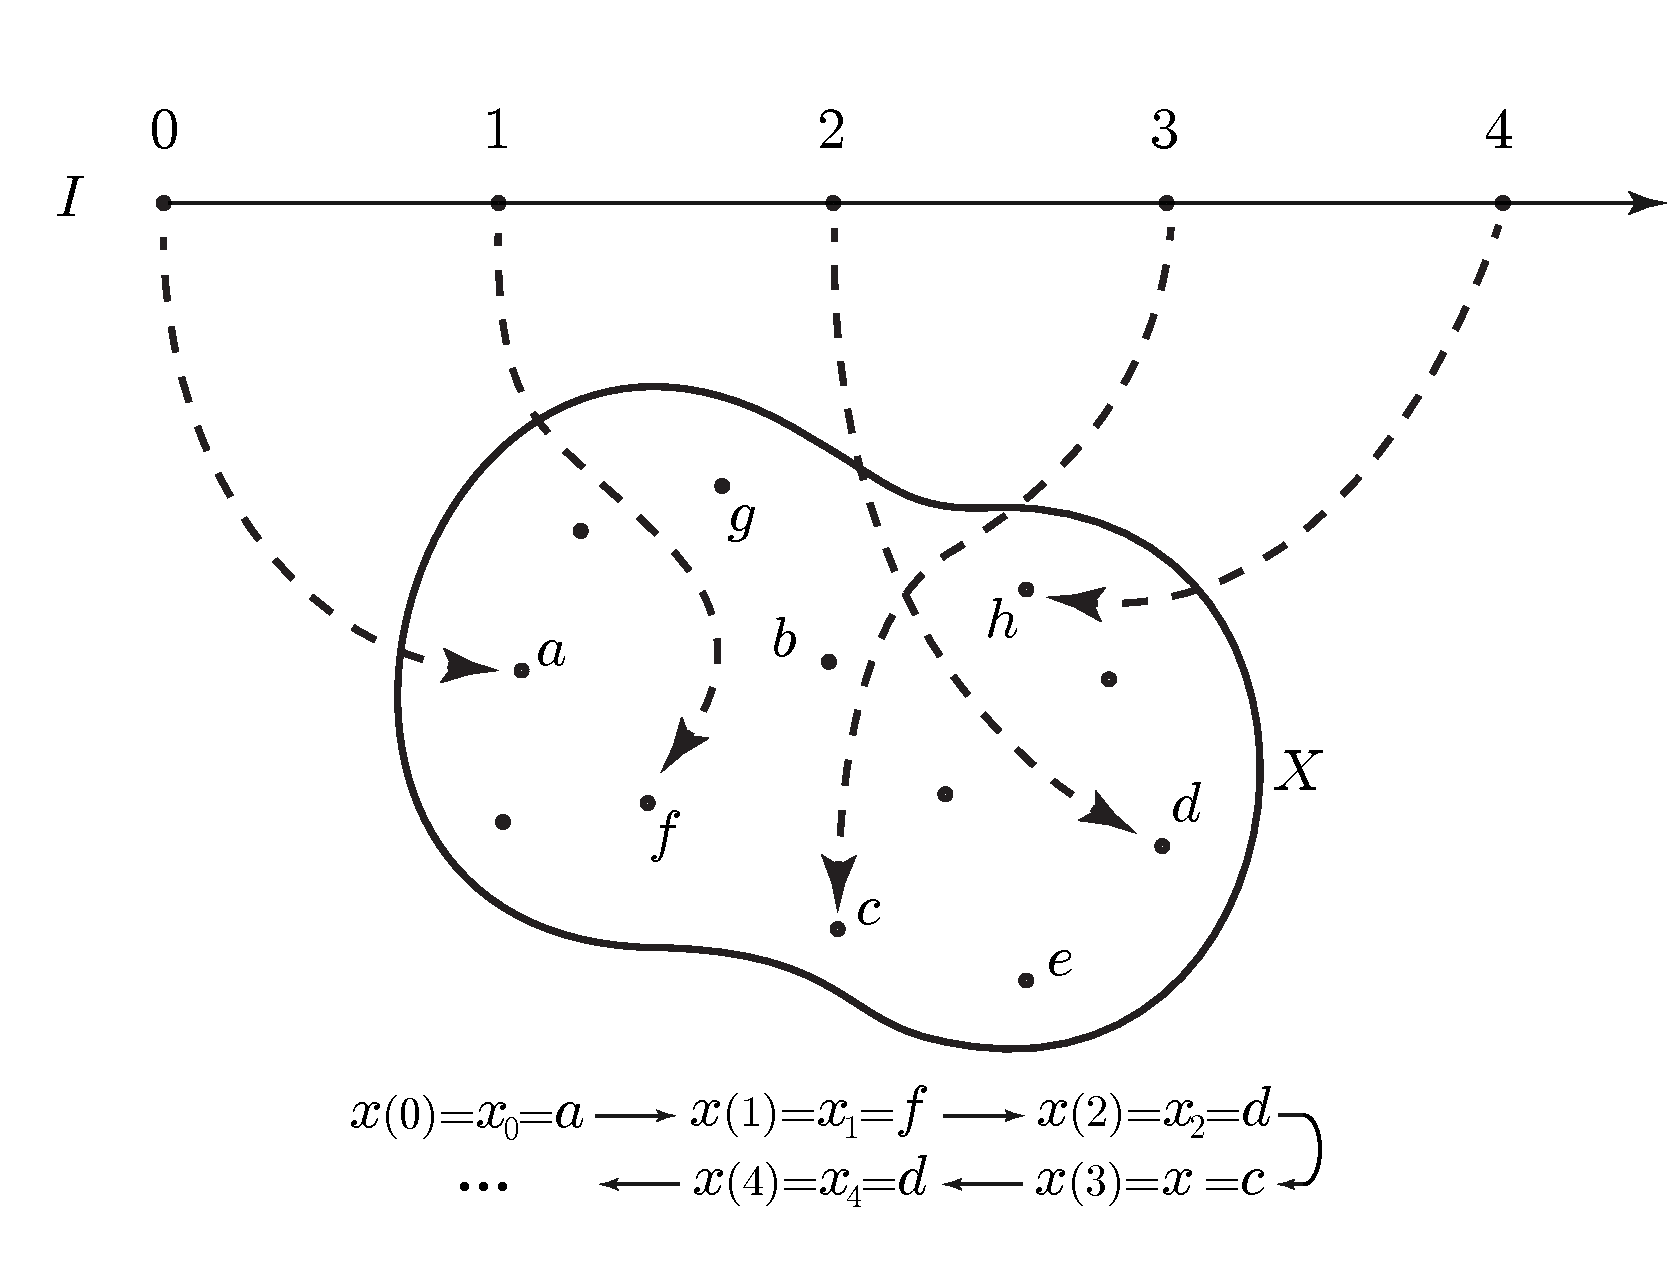
\includegraphics[trim=0cm 0cm 0cm 0cm, clip, scale=0.45]{images/settheorygrafico1.pdf}
\end{center}
È fondamentale che ci sia un \textbf{ordine} su $I$, dato che si vuole confrontare la \textit{posizione} di due elementi della sequenza: un elemento $x_i$ \textit{precede} un altro $x_j$ nella sequenza se gli indici sono tali per cui $i<j$.\\
Per soddisfare la seconda richiesta, ossia che la posizione di un certo elemento nella lista è determinata dalle posizioni degli elementi precedenti, si può pensare di definire la sequenza in modo \textit{ricorsivo}.
Tuttavia, per far ciò, \textit{non} è sufficiente che gli indici siano ordinati. Nello specifico, se $I$ contiene una \textit{sequenza infinita strettamente decrescente}, non siamo sicuri di poter definire ricorsivamente una successione a valori in $X$ indicizzata da $I$.\\
Invece, si può vedere che se $I$ \textit{non} ammette le sequenze infinite strettamente decrescenti, allora le definizioni ricorsive su $I$ sono lecite e permettono di definire univocamente una successione per ogni sequenza di indici! Dobbiamo quindi limitare quali relazioni d'ordine possiamo usare.
\begin{define}[Minimo]
	Se $\left(P,\leq\right)$ è un insieme parzialmente ordinato, $X\neq\emptyset$ un sottoinsieme di $P$ e $a\in X$, allora $a$ è \textbf{minimo}\index{minimo} di $X$ se $a\in X$ e $\forall x\in X,\ a\leq x$. Si indica $a=\min X$.
\end{define}
\begin{define}[Buon ordine]
	Un ordine parziale totale $\leq$ di $P$ è un \textbf{buon ordine} se ogni sottoinsieme $X\neq \emptyset$ di $P$ ha un minimo.
\end{define}
\begin{examples}~{}
	\begin{itemize}
		\item $\left(\naturalset,\leq\right)$ è ben ordinato.
		\item $\integerset,\ \rationalset,\ \realset$ \textit{non} sono ben ordinati rispetto all'ordine canonico $\leq$: tutti ammettono il sottoinsieme $\integerset_{<0}$ degli interi negativi, che non ha minimo.
	\end{itemize}
\end{examples}
\begin{observe}
	Ogni insieme ben ordinato \textit{non} ammette sequenze infinite strettamente decrescenti, in quanto gli elementi della sequenza formano un sottoinsieme e pertanto esso ammette minimo.
\end{observe}
\begin{intuit}
	Possiamo ora capire perché non ha particolarmente senso definire successioni indicizzate, ad esempio, rispetto a $\left(\integerset,<\right)$ o rispetto a $\left(\realset,<\right)$: non ammettendo minimo, non possiamo avere il \textit{passo base} della nostra successione definita ricorsivamente!
\end{intuit}
\begin{digression}
	Il \textbf{teorema del buon ordine}, o anche noto come \textbf{teorema di Zermelo}, afferma che \textit{ogni} insieme non vuoto può essere ben ordinato (rispetto ad un opportuno ordine).\\
	Questo teorema risulta essere vero se si considera valido l'Assioma della Scelta; in realtà, si può ulteriormente mostrare come il teorema del buon ordine risulta essere equivalente, sotto gli Assiomi di Zermelo–Fraenkel, proprio all'Assioma della Scelta!
\end{digression}
Diamo un'ultima definizione, che sarà fondamentale per collegare gli insiemi ben ordinati con gli ordinali.
\begin{define}[Funzioni monotone e isomorfismi d'ordine]
	Siano $\left(P,\leq_P\right)$ e $\left(Q,\leq_Q\right)$ due insiemi parzialmente ordinati. Una funzione $\funz{f}{P}{Q}$ è \textbf{monotona}\index{funzione!monotona} se
	\begin{equation}
		x\leq_P y\implies f(x)\leq_Q f(y)
	\end{equation}
Se una funzione monotona è biettiva e l'\textit{inversa} è monotona, allora $f$ è una \textbf{isotonia}\index{isotonia} o \textbf{isomorfismo d'ordine}.
\end{define}
\section{Ordinali}
Supponiamo di aver preso un insieme degli indici $I$ e, dopo aver posto un buon ordine su di esso, di aver definito una successione nel modo che abbiamo detto nella sezione precedente. Allora, sulla base della definizione intuitiva data nell'introduzione, gli indici scelti fungono proprio da ordinali.\\
Supponiamo ora di prendere un altro insieme di indici $J$ ben ordinati e determinare una successione sulla base di essi. Per questa nuova successione gli elementi di $J$ fanno da ordinale, ma hanno qualcosa in comune con gli indici $I$? Sono gli stessi ordinali o sono ordinali differenti? Potremmo mostrare che c'è un isomorfismo d'ordine tra $I$ e $J$: in questo modo avremmo gli stessi ordinali \textit{a meno di isomorfismo}.\\
Si mostra facilmente che, come ci si aspetterebbe da una funzione chiamata ‘‘isomorfismo'', essere isotonici è una \textbf{relazione di equivalenza} e gli insiemi parzialmente ordinati sono partizionati da essi. Da qui in poi queste classi di equivalenza le chiameremo \textbf{tipi d'ordine}\index{tipo d'ordine}.\\
Georg \textbf{Cantor} (1845 - 1918) definì un numero ordinale proprio come il tipo d'ordine di insiemi \textit{ben ordinati}. Tuttavia, l'indiscutibile appeal intuitivo che questa definizione emana ha due svantaggi:
\begin{enumerate}
	\item I tipi di ordine sono particolarmente ampi: il solo tipo associato all'ordinale $1$, di cui vedremo tra poco la definizione precisa in senso insiemistico, contiene \textbf{tutti} i singoletti, tra cui anche il singoletto $\{1\}$.
	\item In tutte le dimostrazioni che si basano sulle classi di equivalenza è necessario scegliere un rappresentante e controllare che i risultati non dipendono dalla scelta fatta.
\end{enumerate}
Fu John \textbf{von Neumann} (1903-1957)  a proporre un approccio che risolva questi problemi, ma che risulti in tutto e per tutto equivalente alla costruzione originale di Cantor: invece di vedere gli ordinali come classi di equivalenza, definire degli \textit{insiemi canonici} ben ordinati, che chiameremo \textit{ordinali}, e mostrare che ogni insieme ben ordinato è isomorfo ad uno e un solo insieme ordinale. Uno degli aspetti geniali di questa definizione è di definire gli ordinali sulla base degli ordinali che lo precedono, generalizzando ciò che succede per i numeri naturali quando usati per ordinare: un elemento è il \textit{quarto} perché segue il \textit{terzo}, che a sua volta segue il \textit{secondo}, che a sua volta segue il \textit{primo}.\\
Innanzitutto, diamo una definizione formale dei naturali come una famiglia di particolari insiemi costruiti \textit{ricorsivamente dall'insieme vuoto}.
\begin{define}[Numeri naturali]
	I \textbf{numeri naturali} $0,1,2,\ldots$ sono costruiti ricorsivamente nel seguente modo:
	\begin{equation}
		\begin{array}{l}
			0\coloneqq \emptyset\\
			n+1\coloneqq n\cup \left\{n\right\} = \left\{0,\ldots,n\right\}
		\end{array}
	\end{equation}
\end{define}
In altre parole:
\begin{equation*}
	\begin{array}{l}
		0=\left\{\emptyset\right\}\\
		1=\left\{0\right\}=\left\{\emptyset,\left\{\emptyset\right\}\right\}\\
		2=\left\{0,1\right\}=\left\{\emptyset,\left\{\emptyset\right\}, \left\{\emptyset,\left\{\emptyset\right\}\right\}\right\}\\
		\dots
	\end{array}
\end{equation*}
I naturali sono tutti degli insiemi \textit{ben ordinati} e, in particolare, sono anche \textit{transitivi}.
\begin{define}[Transitività]
	Un insieme $T$ è \textbf{transitivo}\index{transitività} se ogni elemento di $T$ è un sottoinsieme di $T$; in altre parole,
	\begin{equation}
		T\subseteq \setpart{T}
	\end{equation}
	o, equivalentemente, se $x\in T$ e $y\in x$, allora $y\in T$.
\end{define}
Possiamo generalizzare la costruzione astratta dei naturali per definire più genericamente i \textit{numeri ordinali}.
\begin{define}[Ordinale]
	Un insieme è un \textbf{ordinale}\index{ordinale} se è transitivo e ben ordinato dalla relazione d'appartenenza $\in$.\\
	Definiamo inoltre una relazione sulla classe di tutti gli ordinali $\mathrm{Ord}$:
	\begin{equation}
		\alpha<\beta\iff\alpha\in\beta
	\end{equation}
\end{define}
\begin{example}
	Per la definizione astratta di naturale, i \textbf{numeri naturali} sono tutti ordinali per definizione.
\end{example}
Dalla sola definizione seguono quasi immediatamente le seguenti proprietà.
\begin{lemmingqed}[Relazioni tra ordinali]
	Valgono le seguenti:
\begin{enumerate}
	\item Se $\alpha$ è un ordinale e $\beta\in\alpha$, allora $\beta$ è un ordinale.
	\item Se $\alpha\neq\beta$ sono ordinali e $\alpha\subsetneqq\beta$, allora $\alpha\in\beta$.
	\item Se $\alpha,\ \beta$ sono ordinali, allora si ha o $\alpha\subseteq\beta$ oppure $\beta\subseteq\alpha$.\qedhere
\end{enumerate}
\end{lemmingqed}
Da questo lemma possiamo ricavare una serie di proprietà importanti:
\begin{itemize}
	\item $<$ è una relazione d'ordine totale nella classe $\mathrm{Ord}$:
	\item Per ogni ordinale $\alpha$ si ha
	\begin{equation*}
		\alpha=\left\{\beta\in\mathrm{Ord} \ \middle| \ \beta<\alpha\right\}
	\end{equation*}
ossia un ordinale contiene \textbf{tutti} gli ordinali che lo precedono.
\item Se $C$ è una classe non vuota di ordinali, allora
\begin{equation*}
	\bigcap C=\inf C\in C
\end{equation*}
è un ordinale
\item Se $X$ è una insieme non vuoto di ordinali, allora
\begin{equation*}
	\bigcup X=\sup X
\end{equation*}
è un ordinale.
\item Per ogni $\alpha$ ordinale, $\alpha\cup\left\{\alpha\right\}$ è un ordinale ed è l'estremo inferiore di tutti gli ordinali che lo seguono.
\begin{equation*}
		\alpha\cup\{\alpha\}=\inf\{\beta\in\mathrm{Ord}\mid\beta>\alpha\}
\end{equation*}
\end{itemize}
\begin{intuit}
	La relazione $<$ indotta da $\in$ sugli ordinali si può vedere come una generalizzazione della relazione d'ordine che conosciamo bene sui naturali. Dopotutto, per essi le due relazioni coincidono!
\end{intuit}
\subsection{Ordinali successori e ordinali limiti}
Data la relazione d'ordine che caratterizzano gli ordinali e sulla base di questi fatti, ha senso definire
\begin{equation*}
	\alpha+1=\alpha\cup\{\alpha\}
\end{equation*}
il \textbf{successore}\index{successore} di $\alpha$.\\
Consideriamo ora un ordinale $\alpha$. Se esiste un ordinale $\beta$ tale per cui $\alpha=\beta+1$, si può dire che $\alpha$ è un \textbf{ordinale successore}. Non è sempre detto che però tale $\beta$ esisti! Un ordinale di questo tipo, per quanto osservato, deve essere successivo a degli ordinali, ma non deve essere il diretto successore di alcun altro ordinale. Utilizzando la terminologia dell'analisi, questo tipo di ordinale è detto \textbf{ordinale limite}\index{ordinale!limite} e
\begin{equation}
	\alpha=\sup\{\beta\in\mathrm{Ord}\mid\beta<\alpha\}=\bigcup\alpha.
\end{equation}
Si considera anche lo \textit{zero} un ordinale limite: si pone $0=\sup\emptyset$.\\
Consideriamo dunque i numeri naturali: ogni numero ha per definizione un successivo e ogni numero è successore di un altro. Segue dunque una domanda esistenziale: c'è qualcosa dopo \textit{tutti} i naturali? La risposta, in teoria degli insiemi, è sì: dopo $0$, $1$, $2$, eccetera, eccetera, si raggiunge un nuovo ordinale, che non è successore di alcun naturale ma che è successivo a tutti: $\omega$.
\begin{define}[Ordinali finiti e transfiniti]
	Si denomina con $\omega$ il più piccolo ordinale limite non zero: esso è il tipo di ordine dei naturali $\naturalset$ e si può identificare con esso.\\
	Gli ordinali prima di $\omega$, ossia i numeri naturali, sono detti ordinali \textbf{finiti}\index{ordinale!finito}, mentre $\omega$ e gli ordinali che seguono sono detti ordinali \textbf{transfiniti}\index{ordinale!transfinito} o \textit{infiniti}.
\end{define}
\begin{intuit}\label{visualizzazioneordinali}
	Come possiamo immaginare gli ordinali transfiniti successivi a $\omega$?\\
	Proviamo prima a guardare agli ordinali da nuovi punti di vista: invece che vederli ‘‘semplicemente'' come insiemi, li possiamo vedere visivamente come sequenze rispetto a $<$, in due modi: la prima è più corretta e fedele alla definizione, mentre la seconda è impropria e - secondo la definizione - errata, ma ci permette di fare alcune intuizioni utili.
	\begin{itemize}
		\item La sequenza di tutti gli ordinali che lo precedono:
		\begin{equation*}
			5\colon 0<1<2<3<4
		\end{equation*}
		\item La sequenza di tutti gli ordinali che lo precedono e l'ordinale stesso:
		\begin{equation*}
			5\colon 0<1<2<3<4\textcolor{red}{<5}
		\end{equation*}
	\end{itemize}
Se $\omega$ è identificato con $\naturalset$, allora le due visualizzazioni sono
	\begin{align*}
		\omega&\colon0<1<2<3<\ldots\\
		\omega&\colon0<1<2<3<\ldots\textcolor{red}{<\omega}
	\end{align*}
La prima visualizzazione coincide la classica rappresentazione dei naturali naturali, mentre la seconda suggerisce qualcos'altro: dopo tutti i naturali ho un elemento nuovo che tuttavia si comporta in modo estremamente simile allo \textit{zero} - dopotutto, non è successore di alcun altro numero, ma ammette un successore.\\
L'idea è quindi di \textbf{rietichettare} $\omega$ con $0'$, $\omega+1$ con $1'$ e così via. In questo modo, un ordinale come $\omega+3$ diventa 
\begin{align*}
	\omega+3&\colon0<1<2<3<\ldots<0'+1'+2'\\
	\omega+3&\colon0<1<2<3<\ldots<0'+1'+2'\textcolor{red}{+3'}
\end{align*}
Questo ragionamento permette di immaginare numeri più complessi: l'ordinale $\omega+\omega$ coincide con due copie dei naturali, la cui seconda copia segue completamente alla destra della prima:
\begin{align*}
	\omega+\omega&\colon0<1<2<3<\ldots<0'<1'<2'<3'<\ldots\\
	\omega+\omega&\colon0<1<2<3<\ldots<0'<1'<2'<3'<\ldots\textcolor{red}{<0''}
\end{align*}
\end{intuit}
Gli ordinali $\omega,\ \omega+1,\ \ldots, \omega\cdot 2,\ \ldots \omega^{\omega}\cdot $ sono tutti ordinali numerabili e riguardando l'ordinamento di insiemi infiniti detti \textit{numerabili}. L'ordinale limite che segue dopo tutti gli ordinali numerabili è indicato come $\omega_1$ ed è il primo ordinale non numerabile.\\ 
Concludiamo la sezione con una definizione che successivamente riprenderemo quando parleremo di cardinalità.
\begin{define}[Insiemi finiti e infiniti.]
	Un insieme $X$ è detto \textbf{finito}\index{insieme!finito} se c'è una biezione tra $X$ e un naturale $n\in\naturalset$, con $n$ inteso come insieme.\\
	Se $X$ non è finito è detto \textbf{infinito}\index{insieme!infinito}.
\end{define}
\subsection{Isomorfismo dell'ordinale con gli insiemi ben ordinati}
Concludiamo senza dare dimostrazione il teorema che permette di concludere la definizione di ordinale secondo von Neumann.
\begin{theoremaqed}[Isotonia tra ordinali e insiemi ben ordinati]
	Ogni insieme ben ordinato è isomorfo ad un unico ordinale.
\end{theoremaqed}
Questo è il motivo per cui si può identificare $\omega$ con $\naturalset$: l'insieme dei naturali è un insieme ben ordinato e si può mostrare l'isomorfismo d'ordine con il più piccolo ordinale limite non nullo.
\subsection{Induzione transfinita}
Ricordiamo uno dei modi per enunciare l'\textit{induzione} sui naturali. 
\begin{theoremaqed}[Induzione]
	Sia $A$ un sottoinsieme di $\naturalset$ e si supponga che
	\begin{enumerate}
		\item $0\in A$.
		\item Se $n\in A$, allora $n+1\in A$.
	\end{enumerate}
	Allora $A=\naturalset$.
\end{theoremaqed}
Con ciò che abbiamo introdotto possiamo generalizzare facilmente questa proprietà agli ordinali anche non finiti.
\begin{theorema}[Induzione transfinita]
	Sia $C$ una classe di ordinali e si supponga che
	\begin{enumerate}
		\item $0\in C$.
		\item Se $\alpha\in C$, allora $\alpha+1\in C$.
		\item Se $\alpha$ è un ordinale limite non zero e si ha $\beta\in C,\ \forall \beta<\alpha$, allora $\alpha\in C$.
	\end{enumerate}
Allora $C=\mathrm{Ord}$.
\end{theorema}
\begin{demonstration}
	Se $C=\mathrm{Ord}$ abbiamo finito. Altrimenti, sia $\alpha$ il più piccolo ordinale\footnote{Possiamo farlo in quanto un ordinale è ben ordinato.} che \textit{non} appartiene a $C$.
	\begin{itemize}
		\item Se $\alpha=0$ si ha subito l'assurdo per l'ipotesi $1$.
		\item Se $\alpha$ è un ordinale successore, allora sia $\beta$ l'ordinale tale per cui $\alpha=\beta+1$: per contronominale sulla ipotesi 2. si ha
		\begin{equation*}
			\alpha=\beta+1\notin C\implies \beta\notin C,
		\end{equation*}
		ma allora essendo $\beta<\alpha$ si ha una contraddizione perché $\alpha$ non è più il più piccolo ordinale non in $C$.
		\item Se $\alpha$ è un ordinale limite non nullo, allora per contronominale sull'ipotesi $3.$ si ha che
		\begin{equation*}
			\exists \beta<\alpha\colon\beta\notin C
		\end{equation*}
		e come prima essendo $\beta<\alpha$ si ha una contraddizione perché $\alpha$ non è più il più piccolo ordinale non in $C$.\qedhere
	\end{itemize}
\end{demonstration}
\subsection{Sequenze e limite}
Diamo ora una definizione di \textit{successione}, che abbiamo finora visto solo intuitivamente.
\begin{define}[Successione]
	Una successione è una funzione il cui dominio è un ordinale $\alpha$. La notazione canonica per una sequenza è
	\begin{equation*}
		\left<a_\xi \ \middle| \ \xi<\alpha\right>
	\end{equation*}
\end{define}
\begin{examples}~
	\begin{itemize}
		\item Una successione finita è una funzione sul dominio finito $\left\{i\in\naturalset\mid i<n\right\}$ per qualche $n\in\naturalset$. Viene anche detta anche \textbf{sequenza di lunghezza} $n$.
		\item Una successione nel senso classico del termine è una funzione su $\naturalset$ o, equivalentemente, sull'ordinale $\omega$. Si può indicare come
			\begin{equation*}
			\left<a_n \ \middle| \ n<\omega\right>
		\end{equation*}
	\end{itemize}
\end{examples}
\begin{define}[Limite di una successione]
	Sia $\alpha>0$ un ordinale limite e sia $\left<\gamma_\xi \ \middle| \ \xi<\alpha\right>$ una successione \textbf{non decrescente} di ordinali, cioè
	\begin{equation*}
		\xi <\eta \implies \gamma_\xi\leq \gamma_\eta.
	\end{equation*}
	Si definisce il \textbf{limite}\index{limite} di una successione
	\begin{equation}
		\lim_{\eta\to \alpha}\gamma_\xi=\sup\left\{\gamma_\xi\mid\xi<\alpha\right\}
	\end{equation}
\end{define}
\subsection{Aritmetica degli ordinali}
\paragraph{Addizione}
\begin{define}[Addizione di ordinali]
	Per ogni ordinale $\alpha$ si ha
	\begin{enumerate}
		\item \textbf{Zero come identità:}
		$\alpha+0=\alpha$
		\item \textbf{Associatività:}
		\begin{equation*}
			\alpha+\left(\beta+1\right)=\left(\alpha+\beta+1\right),\ \forall \beta
		\end{equation*}
		Più in generale, si ha
		\begin{equation*}
			\alpha+\left(\beta+\gamma\right)=\left(\alpha+\beta\right)+\gamma,\ \forall \beta,\ \forall\gamma
		\end{equation*}
		\item \textbf{Somma come limite:}
		\begin{equation*}
			\alpha+\beta=\lim_{\eta\to\beta}\left(\alpha+\eta\right),\ \text{per ogni ordinale limite}\ \beta>0
		\end{equation*}
	\end{enumerate}
\end{define}
\begin{attention}
	L'addizione di ordinali \textbf{non} è commutativa. Ad esempio, $1+\omega=\omega\neq\omega+1$.
\end{attention}
\begin{intuit}
	Prima di dimostrarlo formalmente, cerchiamo di capire intuitivamente perché questo non accade. Riprendendo la prima delle due visualizzazioni introdotta a pag. \pageref{visualizzazioneordinali}, scriviamo $1+\omega$ e $\omega+1$, dove etichettiamo $\omega$ con $0'$.
	\begin{align*}
		1+\omega&\colon0<0'<1'<2'<3'<\ldots\\
		\omega+1&\colon0<1<2<3<\ldots<0'
	\end{align*}
	Notiamo che nel primo caso $0'$ (cioè $\omega$) ha un predecessore, $0$, cosa che normalmente \textit{non} ha; rinominando $n'$ con $n+1$ otteniamo che la sequenza assomiglia in realtà a $\omega$ stesso, cioè possiamo dire che $1+\omega=\omega$. D'altro canto, $\omega+1$ ha un elemento massimo, che è $0'$, mentre $\omega$ non lo ha!
\end{intuit}
\begin{examplewt}[Non commutatività dell'addizione di ordinali]
	Mostriamo che
	\begin{equation*}
		1+\omega=\omega\neq\omega+1
	\end{equation*}
 	Infatti, il termine di sinistra diventa
 	\begin{align*}
 		1+\omega&=\lim_{\eta\to \omega}\left(1+\xi\right)=\sup\left\{1+\xi \ \middle| \ \xi<\omega\right\}=\bigcup_{\xi<\omega}\left\{1+\xi\right\}=\\
 		&=1\cup 2\cup 3\cup \ldots=\{0\}\cup\{0,1\}\cup\{0,1,2\}\cup\ldots\naturalset=\omega
 	\end{align*}
 	e per definizione $\omega<\omega+1$ e dunque sono due ordinali distinti.
\end{examplewt}
In realtà è molto raro che $\alpha+\beta$ sia uguale a $\beta+\alpha$: ciò succede se e solo se $\alpha=\gamma \cdot m$ e $\beta=\gamma \cdot n$ con $\gamma$ ordinale e $m,\ n$ naturali e $\cdot$ la moltiplicazione tra ordinali che vedremo tra poco.
\paragraph{Moltiplicazione}
\begin{define}[Moltiplicazione di ordinali]
	Per ogni ordinale $\alpha$ si ha
	\begin{enumerate}
		\item \textbf{Zero come elemento nullo:}
		$\alpha\cdot0=0$
		\item \textbf{Distributiva da sinistra:}
		\begin{equation*}
			\alpha\cdot\left(\beta+1\right)=\alpha\cdot\beta+\alpha,\ \forall \beta
		\end{equation*}
		\item \textbf{Associativa:}
		\begin{equation*}
			\alpha\cdot\left(\beta\cdot\gamma\right)=\left(\alpha\cdot\beta\right)\cdot\gamma,\ \forall \beta,\ \gamma
		\end{equation*}
		\item \textbf{Prodotto come limite:}
		\begin{equation*}
			\alpha\cdot\beta=\lim_{\eta\to\beta}\left(\alpha\cdot\eta\right),\ \text{per ogni ordinale limite}\ \beta>0
		\end{equation*}
	\end{enumerate}
\end{define}
\begin{attention}
	La moltiplicazione di ordinali \textbf{non} è commutativa e neanche distributiva da destra. Ad esempio, $\left(1+1\right)\cdot\omega=\omega\neq\omega\cdot\left(1+1\right)=\omega+\omega$.
\end{attention}
\begin{examplewt}[Non commutatività della moltiplicazione di ordinali]
	Mostriamo che
	\begin{equation*}
		\left(1+1\right)\cdot\omega=2\omega=\omega\neq\omega\cdot\left(1+1\right)=\omega\cdot 2=\omega+\omega
	\end{equation*}
	Infatti, il termine di sinistra diventa
	\begin{align*}
		\left(1+1\right)\cdot\omega&=2\cdot\omega=\lim_{\eta\to \omega}\left(2\cdot\xi\right)=\sup\left\{2\cdot\xi \ \middle| \ \xi<\omega\right\}=\bigcup_{\xi<\omega}\left\{2\cdot\xi\right\}=\\
		&=2\cdot 0\cup2\cdot 1\cup 2\cdot2\cup 2\cdot3\cup \ldots=0\cup 2\cup 6\cup\ldots=\\
		&=\emptyset\cup\{0,1\}\cup\{0,1,2,3,4,5\}\cup\ldots=\naturalset=\omega
	\end{align*}
	e per definizione $\omega<\omega+\omega$ e dunque sono due ordinali distinti.
\end{examplewt}
\paragraph{Esponenziazione}
\begin{define}[Esponenziazione di ordinali]
		Per ogni ordinale $\alpha$ si ha
	\begin{enumerate}
		\item \textbf{Esponenziazione per zero:}
		$\alpha^0=1$
		\item \textbf{Distributiva dell'esponenziale rispetto all'esponente:}
		\begin{equation*}
			\alpha^{\beta+1}=\alpha^\beta\cdot\alpha,\ \forall \beta
		\end{equation*}
		\item \textbf{Prodotto come limite:}
		\begin{equation*}
			\alpha^{\beta}=\lim_{\eta\to\beta}\left(\alpha^\eta\right),\ \text{per ogni ordinale limite}\ \beta>0
		\end{equation*}
	\end{enumerate}
\end{define}
\paragraph{Aritmetica degli ordinali e aritmetica degli interi}
Abbiamo visto che le operazioni con i numeri ordinali hanno notevoli differenze da queste 
\begin{property}[Aritmetica degli ordinali e aritmetica degli interi]
	Valgono le seguenti proprietà:
	\begin{enumerate}
		\item Se $\beta<\gamma$, allora
		\begin{equation*}
			\alpha+\beta<\alpha+\gamma,\ \forall \alpha.
		\end{equation*}
		\item Se $\alpha<\beta$, allora esiste un unico $\delta$ tale che \begin{equation*}
			\alpha+\delta=\beta.
		\end{equation*}
		\item Se $\beta<\gamma$, allora
		\begin{equation*}
			\alpha\cdot \beta<\alpha\cdot\gamma,\ \forall \alpha>0.
		\end{equation*}
		\item Se $\alpha>0$ e $\gamma$ è un ordinale arbitrario, allora esiste un unico $\beta$ e un unico $\rho<\alpha$ tale che
		\begin{equation*}
			\gamma=\alpha\cdot\beta+\rho.
		\end{equation*}
		\item Se $\beta<\gamma$ e $\alpha>1$, allora
		\begin{equation*}
			\alpha^{\beta}<\alpha^{\gamma}.\qedhere
		\end{equation*}
	\end{enumerate}
\end{property}
\begin{theoremaqed}[Teorema della forma normale di Cantor]
	Ogni ordinale $\alpha>0$ può essere rappresentato unicamente nella forma
	\begin{equation}
		\alpha=\sum_{i=1}^{+\infty}\omega^{\beta_i}\cdot k_i=\omega^{\beta_1}\cdot k_1+\cdot+\omega^{\beta_n}\cdot k_n
	\end{equation}
dove $n\geq 1,\ \alpha\geq \beta_1>\ldots>\beta_n$ e $k_1,\ \ldots, k_n$ sono naturali non nulli.
\end{theoremaqed}
Dal teorema della forma normale è possibile che ci siano degli ordinali $\alpha$ tali che
\begin{equation*}
	\alpha=\omega^{\alpha}
\end{equation*}
Il più piccolo di questi ordinali è indicato con $\epsilon_0$.
\section{Cardinalità}
\begin{comment}

\end{comment}
\begin{define}[Cardinalità]
	Due insiemi $X$ e $Y$ sono \textbf{equipotenti}\index{equipotenza} o \textbf{equinumerosi}\index{equinumerosità}, in simboli
	\begin{equation}
		X\asymp Y
	\end{equation}
	se esiste una corrispondenza \textit{biunivoca} tra i due insiemi.\\
	L'equipotenza è una \textit{relazione di equivalenza} sulle classi di tutti gli insiemi; diciamo che due insiemi $X$ e $Y$ equipotenti hanno la stessa \textbf{cardinalità}\index{cardinalità} e lo indichiamo con
	\begin{equation}
		\abs{X}=\abs{Y}
	\end{equation}
\end{define}

\subsection{Ordine delle cardinalità}
\begin{define}[Iniezione]
	Un insieme $X$ si \textbf{inietta in} $Y$, in simboli 
	\begin{equation}
		X\precsim Y
	\end{equation}
	se esiste una funzione iniettiva $\funz{f}{X}{Y}$; in tal caso scriveremo
	\begin{equation}
		\abs{X}\leq\abs{Y}
	\end{equation}
\end{define}
\begin{corollary}[Inclusione e cardinalità]\label{cardinalitàinclusione}
	Se $X\subseteq Y$, allora $X\precsim Y$ (o in termini di cardinalità, $\abs{X}\leq\abs{Y}$).
\end{corollary}
\begin{demonstration}
	Dire che $X\subseteq Y$ implica l'esistenza dell'inclusione $\incl{\iota}{X}{Y}$, la quale è per definizione una funzione iniettiva.
\end{demonstration}
\begin{attention}\label{cardinalitàugualenonimplicauguaglianzainsiemistica}
	Anche se un sottoinsieme ha la stessa cardinalità dell'insieme a cui appartiene, non è detto che siano uguali; come controesempio basta considerare i numeri naturali $\naturalset$ e numeri pari $2\naturalset$: fra i due c'è una biezione $\funz{\ }{\naturalset}{2\naturalset}$ data da $f(n)=2n$, ma i naturali contengono anche i dispari.\\
	Si può invece affermare che un sottoinsieme \textbf{finito} equipotente all'insieme a cui appartiene deve coincidere con esso.
\end{attention}
La relazione $\precsim$ (o $\leq$ se ci riferiamo alle cardinalità) è una relazione d'\textit{ordine totale}: la relazione riflessiva e transitiva sono immediate, mentre l'antisimmetrica è garantita dal seguente teorema.
\begin{theoremaqed}[Teorema di Cantor-Bernstein-Schröder]
	Se $\abs{X}\leq\abs{Y}$ e $\abs{Y}\leq\abs{X}$, allora $\abs{X}=\abs{Y}$.\\
	Equivalentemente, se esistono due funzioni \textit{iniettive}
	\begin{equation*}
		\funz{f}{X}{Y}\text{ e }\funz{g}{Y}{X}
	\end{equation*}
	allora esiste una funzione \textit{biettiva} $\funz{h}{X}{Y}$.
\end{theoremaqed}
Un'altra conseguenza importante di questo teorema è quella di poter determinare la cardinalità sulla base di sole funzioni \textit{iniettive}.
\begin{examplewt}[Un'applicazione del teorema di Cantor-Bernstein-Schröder]
	L'intervallo $\left[0,1\right]$ ha la cardinalità del continuo; infatti, possiamo considerare le seguenti funzioni iniettive:
	\begin{itemize}
		\item $\incl{\iota}{\left[0,1\right]}{\realset}$ inclusione.
		\item $\funztot{f}{\realset}{\left[0,1\right]}{x}{\frac{2\left(\arctan(x)+\frac{\pi}{2}\right)}{\pi}}$
	\end{itemize}
\end{examplewt}
La seguente proposizione permette invece stabilire una relazione di cardinalità tra dominio e codominio di una funzione \textit{suriettiva}.
\begin{proposition}[La cardinalità del dominio di una funzione suriettiva è maggiore o uguale della cardinalità del codominio]\label{cardinalitàsuriettiva}
	Sia $\surr{g}{Y}{X}$ suriettiva, con $\left(Y,\unlhd\right)$ un insieme ben ordinato. Allora esiste una funzione iniettiva $\funz{f}{X}{Y}$ tale che $g\circ f=id_X$. In altre parole,
	\begin{equation}
		\surr{g}{\left(Y,\unlhd\right)}{X}\implies X\precsim Y \left( \iff \abs{X}\leq\abs{Y}\right).\qedhere
	\end{equation}
\end{proposition}
\begin{demonstration}
	Si definisce $f$ in modo che $f(x)$ è il minimo y$\in Y$, rispetto a $\unlhd$, per cui $g\left(y\right)=x$.
\end{demonstration}
\begin{attention}
	È fondamentale l'ipotesi del buon ordine su $Y$: per insiemi non ben ordinati, la proprietà non si verifica perché non si potrebbe scegliere a priori un elemento da fissare. Tuttavia, se si assume l'Assioma della Scelta come vero allora questa proprietà è verificata per ogni insieme.
\end{attention}
\begin{example}
	Come visto\footnote{Si veda \refChapterOnly{teoriamisura}, pag. \pageref{insiemecantor}.}, dato l'insieme di Cantor $C$ si può definire una funzione $\surr{f}{C}{\left[0,1\right]}$ \textit{suriettiva}; in questo modo, $\abs{C}\geq \left[0,1\right]$ ma, in quanto $C\subseteq \left[0,1\right]$ si ha 
	\begin{equation*}
		\abs{C}=\left|\left[0,1\right]\right|
	\end{equation*}
Questa è anche una conseguenza del teorema di Cantor–Bernstein–Schröder, dato che abbiamo definito (implicitamente o esplicitamente) due funzioni iniettive $\funz{\ }{X}{Y}$ e $\funz{\ }{Y}{X}$.
\end{example}
Ci interessa anche definire una relazione d'\textit{ordine parziale forte} sulla base dell'iniezione precedentemente definita. 
\begin{define}[Iniezione stretta]
	Un insieme $X$ si \textbf{inietta strettamente in} $Y$, in simboli 
	\begin{equation}
		X\precnsim Y
	\end{equation}
	se esiste una funzione iniettiva $\funz{f}{X}{Y}$ ma non esistono funzioni suriettive $\funz{f}{X}{Y}$; in tal caso scriveremo
	\begin{equation}
		\abs{X}<\abs{Y}
	\end{equation}
\end{define}
\begin{observe}
	Si può vedere che
	\begin{equation}
		X \precnsim Y\iff X\precsim Y\wedge X\cancel\asymp Y
	\end{equation}
	o, in termini di cardinalità,
	\begin{equation}
		\abs{X}<\abs{Y}\iff \abs{X}\leq \abs{Y}\wedge \abs{X}\neq\abs{Y}
	\end{equation}
\end{observe}
\subsection{Aritmetica dei cardinali}
Possiamo definire delle \textit{operazioni aritmetiche} con i cardinali; dati $\abs{X}=\kappa$ e $\abs{Y}=\lambda$, si ha
\begin{align}
	\kappa+\lambda&=\abs{X\cup Y} \text{ se }X\text{ e }Y\text{ disgiunti}\\
	\kappa\cdot\lambda&=\abs{X\times Y}\\
	\kappa^{\lambda}&=\abs{X^Y}
\end{align}
dove con $X^Y$ indichiamo l'\textit{insieme delle funzioni} da $Y$ in $X$.\\
Queste operazioni sono ben definite se sono indipendenti dalla scelta di $X$ e $Y$.
\begin{property}[Proprietà dell'aritmetica dei cardinali]
	Valgono le seguenti proprietà:
	\begin{enumerate}
		\item L'addizione $+$ e la moltiplicazione $\cdot$ sono associative, commutative e distributive.
		\item \textbf{Distributività dell'esponenziale rispetto alla base:}
		\begin{equation}
			\left(\kappa\cdot\lambda\right)^{\mu}=\kappa^{\mu}\cdot\lambda^{\mu}
		\end{equation}
		\item \textbf{Distributività dell'esponenziale rispetto all'esponente:}
		\begin{equation}
			\kappa^{\lambda+\mu}=\kappa^{\lambda}\cdot\kappa^{\mu}
		\end{equation}
		\item \textbf{Esponenziale di un esponenziale:}
		\begin{equation}
			\left(\kappa^{\lambda}\right)^{\mu}=\kappa^{\lambda\cdot\mu}
		\end{equation}
		\item Se $\lambda\leq \mu$, allora
		\begin{equation}
			\kappa^{\mu}\leq \lambda^{\mu}
		\end{equation}
		\item Se $0<\lambda\leq \mu$, allora
		\begin{equation}
			\kappa^{\lambda}\leq \kappa^{\mu}
		\end{equation}
		\item Se $\kappa>0$, allora
		\begin{equation}
			\kappa^0=1\qquad 1^{\kappa}=1\qquad 0^\kappa=0
		\end{equation}
	\end{enumerate}
\end{property}
\subsection{Cardinalità dell'insieme delle parti}
Finché operiamo con insiemi finiti, è chiara la differenza tra le dimensioni di due insiemi; la questione è differente se si parla di insiemi infiniti: non sempre è immediata la cardinalità. Ad esempio, i numeri pari e i naturali hanno la stessa cardinalità (basta considerare $f(n)=2n$) come biezione, ma i naturali sembrano molto più grandi.\\
Si potrebbe pensare che tutti gli insiemi infiniti hanno la stessa cardinalità. Il seguente teorema ci mostra come questo \textit{non} sia il caso, e la cardinalità è un aspetto fondamentale dello studio degli insiemi infiniti.
\begin{theorema}[Teorema di Cantor]
	Per ogni insieme $X$ si ha
	\begin{equation}
		X\precnsim\setpart{X}
	\end{equation}
	\begin{equation}
		\abs{X}<\abs{\setpart{X}}
	\end{equation}
\end{theorema}
\begin{demonstration}
	Sia per assurdo $\funz{f}{X}{\setpart{X}}$ una funzione suriettiva e sia
	\begin{equation*}
		Y=\left\{x\in X\mid x\notin f(x)\right\}
	\end{equation*}
	Per la suriettività di $f$, $\exists z\in X$ tale che $f\left(z\right)=Y$; tuttavia, si ha $z\in Y\iff z\notin f\left(z\right)=Y$, il che è assurdo. Segue che $X\nasymp\setpart{X}$.\\
	Invece, la funzione
	\begin{equation*}
		\funztot{f}{X}{\setpart{X}}{x}{\left\{x\right\}}
	\end{equation*}
	è iniettiva e quindi $X\precsim\setpart{X}$. Concludendo, $X\precnsim\setpart{X}$.
\end{demonstration}
\begin{theoremaqed}[Biezione tra {$\setpart{X}$} e insieme delle funzioni da {$X$} in {$\{0,1\}$}]\label{cardinalitàsetpart}
	Dato un qualunque insieme $X$, sia $\setpart{X}$ l'insieme delle parti di $X$ e sia $2^X\coloneqq\left\{0,1\right\}^X$ l'insieme di tutte le funzioni $\funz{\ }{X}{\left\{0,1\right\}}$. Allora esiste una biezione tra $\setpart{X}$ e $2^X$, data da
	\begin{equation}
		\funztot{\Phi}{\setpart{X}}{2^X}{X}{\chi_X}
	\end{equation}
	con $\chi_X$ la \textit{funzione indicatrice} su $X$; l'inversa di tale funzione è la seguente:
	\begin{equation}
		\funztot{\Phi^{-1}}{2^X}{\setpart{X}}{f}{\left\{x\in\ X\mid f(x)=1\right\}}\qedhere
	\end{equation}
\end{theoremaqed}
\begin{demonstration}
	Per il teorema precedente, si ha una biezione tra $\setpart{X}$ e $2^{\abs{X}}\coloneqq\left\{0,1\right\}^{X}$, dunque hanno la stessa cardinalità. Per esponenziazione dei cardinali, si ha
	\begin{equation*}
		\abs{\setpart{X}}=\left|\left\{0,1\right\}^{X}\right|=\left|\left\{0,1\right\}\right|^{\abs{X}}=2^{\abs{X}}\qedhere
	\end{equation*}
\end{demonstration}
\begin{corollary}[Cardinalità dell'insieme delle parti]\label{insiemiparti}
	Se un insieme $X$ ha cardinalità $\abs{X}$, l'insieme delle parti ha cardinalità
	\begin{equation}
		\abs{\setpart{X}}=2^{\abs{X}}
	\end{equation}
\end{corollary}
Il teorema di Cantor si può quindi riformulare come segue
\begin{theoremaqed}[Teorema di Cantor, riformulato]
	Per ogni cardinale $\kappa$ si ha $\kappa<2^{\kappa}$.
\end{theoremaqed}
\subsection{Ordinali e cardinali}
Sappiamo che gli ordinali, per definizione di von Neumann, sono degli insiemi. Possiamo dare una definizione di \textit{numero cardinale} partendo proprio dal concetto di ordinale.
\begin{define}[Cardinale]
	Un ordinale $\alpha$ è detto un \textbf{cardinale}\index{cardinale} se
	\begin{equation}
		\abs{\alpha}\neq\abs{\beta},\ \forall \beta<\alpha
	\end{equation}
\end{define}
Se $W$ è un insieme ben ordinato, sappiamo che esso ha un tipo d'ordine e dunque almeno un ordinale ad esso associato. Allora consideriamo, dato $W$, il suo numero cardinale come
\begin{equation*}
	\abs{W}=\min\{\alpha\in\mathrm{Ord}\mid\abs{W}=\abs{\alpha}\}
\end{equation*}
Ricordiamo che $X$ è \textit{finito} se è in corrispondenza biunivoca con un \textit{ordinale finito} $n\in\naturalset$:
\begin{equation*}
	\abs{X}=\abs{n}
\end{equation*}
Poichè $\abs{n}=\abs{m}\iff n=m$, gli \textit{ordinali finiti} corrispondono ai \textit{cardinali finiti} e quindi $\abs{n}=n$, ossia
\begin{equation*}
	\abs{X}=n
\end{equation*}
L'ordinale $\omega$ è il più piccolo numero cardinale infinito. 
\begin{observe}
	Tutti i cardinali infiniti sono ordinali limiti.
\end{observe}
Gli ordinali infiniti che sono anche cardinali sono chiamati \textbf{aleph}\index{aleph}.
\begin{lemming}[Successori dei cardinali]
	Si può mostrare che per ogni cardinale $\alpha$ c'è un cardinale più grande di esso. Il più piccolo tra quelli più grandi di $\alpha$ viene indicato con $\alpha^{+}$ ed è detto il \textbf{cardinale successore}\index{cardinale!successore}.
\end{lemming}
In particolare, consegue anche che se $X$ è un insieme di cardinali $\sup X$ è un cardinale.\\
Definiamo allora l'enumerazione degli aleph. Indichiamo normalmente $\aleph_{\alpha}$ per i numeri cardinali e $\omega_\alpha$ per il tipo di ordine.
\begin{align*}
	\aleph_0&=\omega_0=\omega\\
	\aleph_{\alpha+1}&=\alpha_{\alpha}^{+}=\omega_{\alpha+1}\\
	\aleph_{\alpha}&=\omega_{\alpha}=\sup\left\{\omega_\beta\mid \beta<\alpha\right\}\quad\text{se}\ \alpha\ \text{è un ordinale limite}
\end{align*}
In questo modo, affermiamo che
\begin{equation}
	\abs{\naturalset}=\aleph_0
\end{equation}
Inoltre, poiché si può mostrare che $\integerset$ e $\rationalset$ sono in biezione con i naturali, anche loro hanno cardinalità $\aleph_0$.
\begin{observe}
	Dalla definizione si nota un fatto fondamentale: ci possono essere più ordinali per uno stesso cardinale. Come mai?\\
	Gli ordinali descrivono in che maniera (a meno di rietichettare i miei elementi) posso ordinare un insieme, mentre i cardinali sono una misura della dimensione di tale insieme.\\ Finché ci limitiamo ai naturali, come ben sappiamo, non c'è differenza tra ordinale e cardinale. Anzi! Ad ogni numero naturale associamo un solo ordinale e un solo cardinale - ad esempio, se devo ordinare l'insieme $\{1,2,3,4\}$ - che ha cardinalità $4$ - non importa se metto prima il 2 dell'1 o il 3 dopo il 4, dato che rinominando gli elementi ottengo sempre l'ordine canonico $0<1<2<3$.\\
	Caso differente è per gli insiemi infiniti. Ad esempio, sui naturali posso avere l'ordinamento canonico $\omega$, ma posso anche riordinarli mettendo prima tutti i naturali dispari seguiti da tutti i naturali pari:
	\begin{equation*}
		1<3<5<7<9<\ldots<2<4<6<8<10<\ldots
	\end{equation*}
	Questo ordinamento quale ha tipo d'ordine $\omega\cdot 2\neq \omega$. Tuttavia, entrambi sono ordinamenti dei naturali e quindi hanno cardinalità $\aleph_0$.
\end{observe}
La somma e il prodotto di aleph è abbastanza triviale, dato che si può mostrare che:
\begin{equation*}
	\aleph_{\alpha}+\aleph_{\beta}=\aleph_{\alpha}\cdot\aleph_{\beta}=\max\{\aleph_{\alpha},\aleph_{\beta}\}
\end{equation*}
\subsection{Cardinalità del continuo}
Abbiamo definito i cardinali per insiemi \textit{ben ordinati}, basandoci sugli ordinali. In realtà, se supponiamo l'\textit{Assioma di Scelta}, allora \textit{ogni insieme} è ben ordinato e quindi possiamo parlare di cardinali in generale in $\mathsf{ZFC}$, anche per insiemi come i \textit{reali}.
\begin{theoremaqed}[Cantor]
L'insieme dei numeri reali non è numerabile, ossia è un insieme infinito che non è in corrispondenza biunivoca con i naturali.
\end{theoremaqed}
Indichiamo con $\mathfrak{c}$ la \textbf{cardinalità dei reali} o \textbf{cardinalità del continuo}\index{cardinalità!del continuo}:
\begin{equation}
	\abs{\realset}=\mathfrak{c}
\end{equation}
Che valore ha questa cardinalità?\\
Poiché siamo in grado di calcolare la cardinalità dell'insieme delle parti di insiemi per il corollario \ref{insiemiparti}, si ha che $\abs{\setpart{\naturalset}}=2^{\aleph_{0}}$.\\
Dato che ogni numero reale è l'estremo superiore di un'opportuna sequenza di razionali minori di essa, cioè
\begin{equation*}
	r=\sup\{q\in\rationalset\mid q<r\},
\end{equation*}
si ha che la cardinalità dei reali deve essere minore dell'insieme delle sequenze in $\rationalset$, che ha cardinalità pari all'insieme delle parti di $\rationalset$, ovvero
\begin{equation*}
	\mathfrak{c}\leq\abs{\setpart{\rationalset}}=2^{\aleph_0}
\end{equation*}
D'altro canto, l'insieme di Cantor\footnote{Si veda \refChapterOnly{teoriamisura}, pag. \pageref{insiemecantor}.} si vede che è in corrispondenza diretta con tutte le sequenze di $0$ e $2$ e la cardinalità coincide con quella di $2^{\aleph_0}$. Poiché Cantor è un sottoinsieme dei reali, si ha
\begin{equation*}
	\mathfrak{c}\geq \abs{C}=2^{\aleph_0}
\end{equation*}
e quindi si può concludere per Cantor-Bernstein-Schröder che
\begin{equation*}
	\mathfrak{c}=2^{\aleph_0}
\end{equation*}
Una peculiarità di questo cardinale è che nella teoria $\mathsf{ZFC}$ \textit{non} è chiaro dove si posizioni nella gerarchia degli $\aleph$, ma Cantor formulò una congettura a riguardo: non ci sono insiemi la cui cardinalità è compresa tra quella degli interi e quella dei reali; in altre parole,
\begin{equation}
	(\mathsf{CH})\quad 2^{\aleph_0}=\aleph_1
\end{equation}
L'\textbf{ipotesi del continuo} ($\mathsf{CH}$) non può essere provata o confutata nel sistema di $\mathsf{ZFC}$.\\
Cos'è, invece, la cardinalità dell'insieme delle parti dei reali?\label{cardinalitàsetpartreali}
\begin{equation*}
\abs{\setpart{\realset}}=2^{\mathfrak{c}}
\end{equation*}
Sappiamo che è un numero \textit{ancora più grande} della cardinalità del continuo, ma non è per nulla facile capire cos'è. \\
Dato che ciò esenta gli scopi che ci siamo prefissi per questa appendice - che già di per sé è un esteso (e non necessario) approfondimento di teoria degli insiemi\footnote{Nel caso avessimo sbagliato in qualche punto, qualche logico ci illumini per favore. Io manco ho seguito \textsc{Logica}.} scritto per spiegare qualche termine usato nel capitolo di Teoria della Misura - lasciamo ad un eventuale lettore curioso qualche spunto a riguardo:
\begin{itemize}
	\item \textbf{Beth number}\\ \textcolor{redill}{\url{https://en.wikipedia.org/wiki/Beth_number}}
	\item \textbf{What is known about the power set of the real number line?}\\ \textcolor{redill}{\url{https://math.stackexchange.com/a/94000/875294}}
\end{itemize}
%% SVN info for this file
\svnidlong
{$HeadURL$}
{$LastChangedDate$}
{$LastChangedRevision$}
{$LastChangedBy$}

\chapter{Note aggiuntive}
\labelAppendix{footnotes}
\addtocontents{define}{\noindent\textls{\textsc{\textcolor{reddo}{Appendice C:}
\nowtitle}}
}{}
\addtocontents{theorema}{\noindent\textls{\textsc{\textcolor{reddo}{Appendice C:}
			\nowtitle}}
}{}
\begin{introduction}
‘‘... and they don't stop coming.''
\begin{flushright}
	\textscsl{Smash Mouth,} sorpresi che ci siano anche delle note aggiuntive dopo quasi trecento pagine di appunti.
\end{flushright}
\end{introduction}

\noindent Riportiamo alcune note, precisazioni e dimostrazioni complementari agli argomenti dei capitoli principali.\\
Quanto indicato con il simbolo ⋆ sono degli \textit{approfondimenti non necessari} - ma possono essere comunque utili ed interessanti per un lettore curioso.
\section{Capitolo 7: magnetostatica}
\subsection{Area di una superficie delimitata da una curva piana chiusa}\label{AreaCurvaDelimitata}
\begin{lemming}[Area di una superficie delimitata da una curva piana chiusa]
	Data una curva $\gamma$ piana, chiusa, liscia a tratti, semplice e orientata positivamente, con parametrizzazione $\vba{r}$, si ha che il vettore area per la superficie piana racchiusa da $\gamma$ è
	\begin{equation}
		\tcboxmath[colback=yellowpastellow!30!white,colframe=yelloworange!85!black,drop fuzzy shadow, nobeforeafter, math upper, tcbox raise base, enhanced]{\Sigma\vbh{u}_n=\frac{1}{2}\int_{\gamma}\vba{r}\cross d\vba{s}}
	\end{equation}
\end{lemming}
\begin{demonstration}
	Dato che la nostra curva $\gamma$ è una \textit{curva di Jordan}, ossia $\gamma$ divide il piano in una componente connessa \textit{interna} limitata e una \textit{esterna} limitata, ha senso porre un sistema di riferimento in \textit{coordinate polari}, con origine un punto arbitrariamente scelto nella componente del piano interna alla curva: se $\theta$ è l'angolo azimutale e $\rho$ la distanza dall'origine, si ha
	\begin{equation*}
		\begin{cases}
			x=\rho \cos\theta\\
			y=\rho \sin\theta
		\end{cases}
	\end{equation*}
	La curva $\gamma$ può essere quindi parametrizzata come 
	\begin{equation*}
		\vba{r}(\theta)=\rho(\theta)\cos \theta\vbh{u}_x+\rho(\theta)\sin \theta\vbh{u}_y
	\end{equation*}
	su $\left[\theta_1,\theta_2\right]$ e tale per cui $\vba{r}(\theta_1)=\vba{r}(\theta_2)$; $\rho(\theta)$ descrive la distanza dall'origine. La velocità risulta
	\begin{align*}
		\vbd{r}(\theta)&=\dv{t}\left(\rho(\theta)\cos \theta\right)\vbh{u}_x+\dv{t}\left(\rho(\theta)\sin \theta\right)\vbh{u}_y=\\
		&=\left(\dot{\rho}(\theta)\cos \theta-\rho(\theta)\sin \theta\right)\vbh{u}_x+\left(\dot{\rho}(\theta)\sin \theta+\rho(\theta)\cos \theta\right)\vbh{u}_y
	\end{align*}
	Poiché l'elemento di area dalle coordinate cartesiane alle coordinate polari diventa
	\begin{equation*}
		dA=dxdy=\rho d\rho d\theta,
	\end{equation*}
	l'area delimitata dalla curva $\gamma$ è
	\begin{equation*}
		\Sigma=\int_{\Sigma}dxdy=\int_{0}^{2pi}\int_{0}^{\rho(\theta)}\int \rho d\rho d\theta= \int_{0}^{2pi}\frac{1}{2}\eval{\rho}_{0}^{\rho(\theta)} d\theta=\frac{1}{2}\int_{0}^{2pi}\rho^2(\theta)d\theta
	\end{equation*}
	Ora, calcolando il prodotto vettoriale 
	\begin{align*}
		\vba{r}\cross\vbd{r}&=
		\begin{vmatrix}
			\vba{u}_x & \vba{u}_y & \vba{u}_z\\
			\rho(\theta)\cos \theta & \rho(\theta)\sin \theta & 0\\
			\dot{\rho}(\theta)\cos \theta-\rho(\theta)\sin \theta & \dot{\rho}(\theta)\sin \theta+\rho(\theta)\cos \theta & 0
		\end{vmatrix}=\\
	&=\left(\rho^2\cos^2\phi + \rho \dot{\rho}\sin\phi\cos\phi-\rho \dot{\rho}\sin\phi\cos\phi+\rho^2\sin^2\phi\right)\vbh{u}_z=\rho^2\left(\phi\right)\vbh{u}_z
	\end{align*}
	Poichè il versore normale ad una superficie nel piano $xy$ quale $\Sigma$ è $\vbh{u}_z$ è immediato trovare che
	\begin{equation*}
		\frac{1}{2}\int_{\gamma}\vba{r}\cross d\vba{r}=\frac{1}{2}\int_{\phi_1}^{\phi_2}\vba{r}\cross\vbd{r}d\phi=\frac{1}{2}\int_{\phi_1}^{\phi_2}\rho^2\left(\phi\right)d\phi\vbh{u}_z=\Sigma\vbh{u}_z\qedhere
	\end{equation*} 
\end{demonstration}
\begin{observe} % TO DO: metterci teorema di stokes? https://en.wikipedia.org/wiki/Green%27s_theorem#Area_calculation
	% https://en.wikipedia.org/wiki/Vector_area
	% https://math.stackexchange.com/questions/74583/proof-that-vector-area-is-a-boundary-integral
	Tale risultato è equivalente a calcolare l'area di una superficie bidimensionale utilizzando il \textbf{teorema di Gauss-Green} e dunque è un'ulteriore corollario del \textit{teorema di Stokes}.\\
	In quanto tale, si può mostare che la relazione scritta vale per una \textit{qualunque} superficie che ha come bordo una determinata curva: il vettore area è determinato \textit{esclusivamente} dal bordo della superficie.
\end{observe}
\section{Capitolo 11: oscillazioni elettriche e correnti alternate}
\subsection{Fasori}\label{fasori}
\begin{define}[Fasore]
	Data una grandezza sinusoidale
	\begin{equation*}
		\xi(t)=A\cos(\omega t+\oldphi)
	\end{equation*}
	dove l'\textit{ampiezza} $A$, la pulsazione $\omega$ e la fase $\oldphi$ sono costanti temporali, la sua \textbf{rappresentazione analitica}\index{rappresentazione analitica} o \textbf{fasore}\index{fasore} è
	\begin{equation}
		\tcboxmath[colback=yellowpastellow!30!white,colframe=ceruleancrayola!85!black,drop fuzzy shadow, nobeforeafter, math upper, tcbox raise base, enhanced]{\hat{\xi}(t)=A\cos(\omega t+\oldphi)+iA\sin(\omega t+\oldphi)=Ae^{i(\omega t+\oldphi)}=Ae^{i\oldphi}e^{i\omega t}}
	\end{equation}
\end{define}
Il fasore può essere rappresentato nel \textit{piano complesso di Argand-Gauss} come un vettore di lunghezza $A$ e angolo $\oldphi$, che ruota con velocità angolare $\omega$.
%TODO: grafico
In realtà, in molti contesti il termine di rotazione $e^{i\omega t}$ risulta essere comune ad altri fasori e pertanto le operazioni che andremo a fare si possono eseguire direttamente sui termine $Ae^{i\oldphi}$ - sarà poi facile reinserire $e^{i\omega t}$ alla fine dei calcoli. Di conseguenza, potrà essere utile passare alla \textit{rappresentazione vettoriale} per le nostre operazioni tra fasori con la stessa pulsazione.
\begin{attention}
	Per il motivo sopracitato, in diversi contesti il termine ‘‘\textit{fasore}'' fa riferimento esclusivamente a $Ae^{i\theta}$.
\end{attention}
Si osservi che, poiché la grandezza originale non è altro che la \textit{parte reale} del fasore...
\begin{equation}
	\tcboxmath[colback=yellowpastellow!30!white,drop fuzzy shadow, nobeforeafter, math upper, tcbox raise base, enhanced]{\xi(t)=\Re{\hat{\xi}(t)}}
\end{equation}
... nella rappresentazione vettoriale dei fasori la grandezza originale è la proiezione sulla retta dei reali.
\begin{notate}
	Tralasciando il termine di rotazione, un fasore di ampiezza $A$ e angolo $\oldphi$ si indica come
	\begin{equation}
		\xi=A\angle\oldphi
	\end{equation}
\end{notate}
\paragraph{Moltiplicazione per una costante (scalare)}
La \textbf{moltiplicazione} di un fasore
\begin{equation*}
	\hat{\xi}(t)=Ae^{i\oldphi}e^{i\omega t}
\end{equation*}
per una costante scalare complessa
\begin{equation*}
	\hat{k}=Be^{i\theta}
\end{equation*}
è ancora un fasore, che modifica l'\textit{ampiezza} e la \textit{fase} del fasore originale.
\begin{empheq}[box=\tcmathboxgeneral]{gather}
	\hat{k}\hat{\xi}(t)=Be^{i\theta}\cdot Ae^{i\oldphi}e^{i\omega t}=ABe^{i(\oldphi+\theta)}e^{i\omega t}\\
	k\xi(t)=AB\cos(\omega t+(\oldphi+\theta))
\end{empheq}
%TODO: grafico
In notazione fasoriale:
\begin{equation}
	\tcboxmath[colback=yellowpastellow!30!white,drop fuzzy shadow, nobeforeafter, math upper, tcbox raise base, enhanced]{\hat{k}\cdot A\angle\oldphi=AB\angle\left(\oldphi+\theta\right)}
\end{equation}
\paragraph{Somma di fasori}
La \textbf{somma} di due fasori
\begin{align*}
	\hat{\xi_1}(t)=A_1e^{i\oldphi_1}e^{i\omega t}&&\hat{\xi_2}(t)=A_2e^{i\oldphi_2}e^{i\omega t}
\end{align*}
è ancora un fasore.
\begin{empheq}[box=\tcmathboxgeneral]{gather}
	\hat{\xi_1}(t)+\hat{\xi_2}(t)=A_1e^{i\oldphi_1}e^{i\omega t}+A_2e^{i\oldphi_2}e^{i\omega t}=\left(A_1e^{i\oldphi_1}+A_2e^{i\oldphi_2}\right)e^{i\omega t}=A_3e^{i\oldphi_3}e^{i\omega t}\\
	\xi_1(t)+\xi_2(t)=A_3\cos(\omega t+\oldphi_3)
\end{empheq}
dove
\begin{align*}	A_3^2&=\left(A_1^2\cos\oldphi_1+A_2^2\cos\oldphi_1\right)^2+\left(A_1^2\sin\oldphi_1+A_2^2\sin\oldphi_1\right)^2\\
	&=A_1^2+A_2^2+2A_1A_2\cos(\oldphi_1-\oldphi_2)
\end{align*}
\begin{equation*}
	\oldphi_3=\begin{cases}
		\textrm{sgn}(A_1 \sin(\oldphi_1)  + A_2 \sin(\oldphi_2)) \frac{\pi}{2}&\text{se}\ A_1 \cos\oldphi_1 + A_2 \cos\oldphi_2 = 0\\
		\arctan\left(\frac{A_1 \sin\oldphi_1 + A_2 \sin\oldphi_2}{A_1 \cos\oldphi_1 + A_2 \cos\oldphi_2}\right)&\text{se}\ A_1 \cos\oldphi_1 + A_2 \cos\oldphi_2 >0\\
		\pi + \arctan\left(\frac{A_1 \sin\oldphi_1 + A_2 \sin\oldphi_2}{A_1 \cos\oldphi_1 + A_2 \cos\oldphi_2}\right) &\text{se}\ A_1 \cos\oldphi_1 + A_2 \cos\oldphi_2 <0
	\end{cases}
\end{equation*}
%TODO: grafico
In notazione fasoriale:
\begin{equation}
	\tcboxmath[colback=yellowpastellow!30!white,drop fuzzy shadow, nobeforeafter, math upper, tcbox raise base, enhanced]{A_1\angle\oldphi_1+A_2\angle\oldphi_2=A_3\angle\oldphi_3}
\end{equation}
Alternativamente, si può fare la \textit{somma vettoriale} dei vettori di coordinate
\begin{align*}
	\hat{\xi_1}(t)=\left(A_1\cos(\omega t+\oldphi_1),A_1\sin(\omega t+\oldphi_1)\right)&&
	\hat{\xi_2}(t)=\left(A_2\cos(\omega t+\oldphi_2),A_2\sin(\omega t+\oldphi_2)\right)
\end{align*}
per produrre il vettore risultante
\begin{equation*}
	\hat{\xi_1}(t)+\hat{\xi_2}(t)=\left(A_3\cos(\omega t+\oldphi_3),A_3\sin(\omega t+\oldphi_3)\right)
\end{equation*}
\paragraph{Derivata e integrale}
La \textbf{derivata temporale} o l'\textbf{integrale} rispetto a $t$ di un fasore produce un altro fasore.
\begin{empheq}[box=\tcmathboxgeneral]{gather}
	\dv{t} \hat{\xi}(t)=\dv{t}\left(Ae^{i\oldphi}e^{i\omega t}\right)=Ae^{i\oldphi}i\omega e^{i\omega t}=\omega Ae^{i\oldphi}e^{i\frac{\pi}{2}} e^{i\omega t}=\omega Ae^{i(\oldphi+\frac{\pi}{2})}e^{i\omega t}\\
	\dv{t} \xi(t)=\omega A\cos\left(\omega t+\theta+\frac{\pi}{2}\right)
\end{empheq}
In altre parole, \textit{derivare} un fasore temporalmente è equivalente a moltiplicare per la costante scalare $i\omega$.
\begin{equation}
	\tcboxmath[colback=yellowpastellow!30!white,drop fuzzy shadow, nobeforeafter, math upper, tcbox raise base, enhanced]{\dv{t} \hat{\xi}(t)=i\omega\hat{\xi}(t)=e^{i\frac{\pi}{2}}\omega\hat{\xi}(t)}
\end{equation}
In notazione fasoriale:
\begin{equation}
	\tcboxmath[colback=yellowpastellow!30!white,drop fuzzy shadow, nobeforeafter, math upper, tcbox raise base, enhanced]{\dv{t} A\angle\oldphi=i\omega \cdot A\angle\oldphi=\omega A\angle\left(\oldphi+\frac{\pi}{2}\right)}
\end{equation}
In modo analogo, integrare un fasore temporalmente è equivalente a dividere per la costante scalare $i\omega$.
\begin{equation}
	\tcboxmath[colback=yellowpastellow!30!white,drop fuzzy shadow, nobeforeafter, math upper, tcbox raise base, enhanced]{\int \hat{\xi}(t) dt=\frac{1}{i\omega}\hat{\xi}(t)=\frac{e^{-\frac{\pi}{2}}}{\omega}\hat{\xi}(t)}
\end{equation}
In notazione fasoriale:
\begin{equation}
	\tcboxmath[colback=yellowpastellow!30!white,drop fuzzy shadow, nobeforeafter, math upper, tcbox raise base, enhanced]{\int A\angle\oldphi dt=\frac{1}{i\omega} \cdot A\angle\oldphi=\frac{A}{\omega}\angle\left(\oldphi-\frac{\pi}{2}\right)}
\end{equation}
\paragraph{Rapporto tra fasori}
Il \textbf{rapporto} tra due fasori
\begin{align*}
	\hat{\xi_1}(t)=A_1e^{i\oldphi_1}e^{i\omega t}&&\hat{\xi_2}(t)=A_2e^{i\oldphi_2}e^{i\omega t}
\end{align*}
prende il nome di \textbf{impendenza}\index{impendenza}:
\begin{equation}
	 \tcboxmath[colback=yellowpastellow!30!white,drop fuzzy shadow, nobeforeafter, math upper, tcbox raise base, enhanced]{Z=\frac{\hat{\xi_1}(t)}{\hat{\xi_2}(t)}=\frac{A_1e^{i\oldphi_1}\Ccancel[red]{e^{i\omega t}}}{A_2e^{i\oldphi_2}\Ccancel[red]{e^{i\omega t}}}=\frac{A_1}{A_2}e^{i(\oldphi_1-\oldphi_2)}}
\end{equation}
Tuttavia, \textit{non} è un fasore, perché non corrisponde ad una grandezza sinusoidale variabile nel tempo.
%% SVN info for this file
\svnidlong
{$HeadURL$}
{$LastChangedDate$}
{$LastChangedRevision$}
{$LastChangedBy$}

\chapter{Proprietà varie ed eventuali}
\labelAppendix{proprietà}

\begin{introduction}
‘‘La Matematica consiste di fatti veri riguardanti oggetti immaginari.''
\begin{flushright}
	\textscsl{Philip Davis e Reuben Hersh,} matematici immaginari con opinioni vere.
\end{flushright}
\end{introduction}

Riportiamo alcune proprietà utili per il lettore.
\section{Immagine e controimmagine}
Data una funzione $\funz{f}{X}{Y}$, per ogni sottoinsieme $A\subseteq X$ e $B\subseteq Y$ valgono le seguenti proprietà:
\begin{center}
	\begin{tabular}{l|l}
	\multicolumn{1}{c|}{\textbf{Immagine}} 	& \multicolumn{1}{c}{\textbf{Controimmagine}}\\ \hline
	$f(X)\subseteq Y$				& $f^{-1}(Y) = X$ 	\\ 
	$f(f^{-1}(Y)) = f(X)$			& $f^{-1}(f(X))= X$ \\
	$f(f^{-1}(B)) \subseteq B$ \footnotemark{}	& $f^{-1}(f(A)) \supseteq A$ \footnotemark{}	\\
	$f(f^{-1}(B)) = B \cap f(X)$	& $(f \mid_A)^{-1}(B) = A \cap f^{-1}(B)$											\\
	$f(f^{-1}(f(A))) = f(A)$		& $f^{-1}(f(f^{-1}(B))) = f^{-1}(B)$											\\
	$f(A) = \emptyset \iff A = \emptyset$	&  $f^{-1}(B) = \emptyset \iff B \subseteq Y \setminus f(X)$					\\
	$f(A) \supseteq B \iff \exists C \subseteq A \colon f(C) = B$ & $f^{-1}(B) \supseteq A \iff f(A) \subseteq B$\\
	$f(A) \supseteq f(X \setminus A) \iff f(A) = f(X)$ & $f^{-1}(B) \supseteq f^{-1}(Y \setminus B) \iff f^{-1}(B) = X$\\
	$f(X \setminus A) \supseteq f(X) \setminus f(A)$ & $f^{-1}(Y \setminus B) = X \setminus f^{-1}(B)$ \\
	$f(A \cup f^{-1}(B)) \subseteq f(A) \cup B$ & $f^{-1}(f(A) \cup B) \supseteq A \cup f^{-1}(B)$ \\
	$f(A \cap f^{-1}(B)) = f(A) \cap B$ & $f^{-1}(f(A) \cap B) \supseteq A \cap f^{-1}(B)$ \\
	\multicolumn{2}{c}{$f(A) \cap B = \emptyset \iff A \cap f^{-1}(B) = \emptyset$}
\end{tabular}
\addtocounter{footnote}{-2}
\stepcounter{footnote}\footnotetext{Uguale se $B\subseteq f(X)$, cioè se $f$ \textit{suriettiva}.}
\stepcounter{footnote}\footnotetext{Uguale se $f$ \textit{iniettiva}.}	
\end{center}

Date le funzioni $\funz{f}{X}{Y}$ e $\funz{f}{Y}{Z}$, valgono le seguenti proprietà:
\begin{itemize}
	\item $(g \circ f)(A) = g(f(A))$
	\item $(g \circ f)^{-1}(C) = f^{-1}(g^{-1}(C))$
\end{itemize}
Data una funzione $\funz{f}{X}{Y}$ e dati i sottoinsiemi $A_1,\ A_2\subseteq X$ e $B_1,\ B_2\subseteq Y$ valgono le seguenti proprietà:
\begin{center}
	\begin{tabular}{l|l}
		\multicolumn{1}{c|}{\textbf{Immagine}} 	& \multicolumn{1}{c}{\textbf{Controimmagine}}\\ \hline
		$A_1 \subseteq A_2 \implies f(A_1) \subseteq f(A_2)$	& $B_1 \subseteq B_2 \implies f^{-1}(B_1) \subseteq f^{-1}(B_2)$ 	\\ 
		$f(A_1 \cup A_2) = f(A_1) \cup f(A_2)$	& $f^{-1}(B_1 \cup B_2) = f^{-1}(B_1) \cup f^{-1}(B_2)$ \\
		$f(A_1 \cap A_2) \subseteq f(A_1) \cap f(A_2)$ \footnotemark{}	& $f^{-1}(B_1 \cap B_2) = f^{-1}(B_1) \cap f^{-1}(B_2)$	\\
		$f(A_1 \setminus A_2) \supseteq f(A_1) \setminus f(A_2)$  \footnotemark{} & $f^{-1}(B_1 \setminus B_2) = f^{-1}(B_1) \setminus f^{-1}(B_2)$
	\end{tabular}
\addtocounter{footnote}{-2}
\stepcounter{footnote}\footnotetext{\label{note1}Uguale se $f$ \textit{iniettiva}.}
\stepcounter{footnote}\footnotetext{Si veda \ref{note1}.}
\end{center}
Data una funzione $\funz{f}{X}{Y}$ e date le famiglie di sottoinsiemi $\{A_i\}\subseteq\setpart{X}$ e $\{B_i\}\subseteq\setpart{Y}$ (con $I$ un insieme di indici anche \textit{infinito} o \textit{non numerabile}) valgono le seguenti proprietà:
\begin{center}
	\begin{tabular}{l|l}
		\multicolumn{1}{c|}{\textbf{Immagine}} 	& \multicolumn{1}{c}{\textbf{Controimmagine}}\\ \hline
		$\displaystyle f\left(\bigcup_{i\in I}A_i\right) = \bigcup_{i\in I} f(A_i)$	& $\displaystyle f^{-1}\left(\bigcup_{i\in I}B_i\right) = \bigcup_{i\in I} f^{-1}(B_i)$ 	\\ 
		$\displaystyle f\left(\bigcap_{i\in I}A_i\right) \subseteq \bigcap_{i\in I} f(A_i)$ \footnotemark{}	& $\displaystyle f^{-1}\left(\bigcap_{i\in I}B_i\right) = \bigcap_{i\in I} f^{-1}(B_i)$
	\end{tabular}
\addtocounter{footnote}{-1}
\stepcounter{footnote}\footnotetext{Si veda \ref{note1}.}
\end{center}
\section{Modi di convergenza}
Lo schema riassuntivo è nella pagina successiva.
	%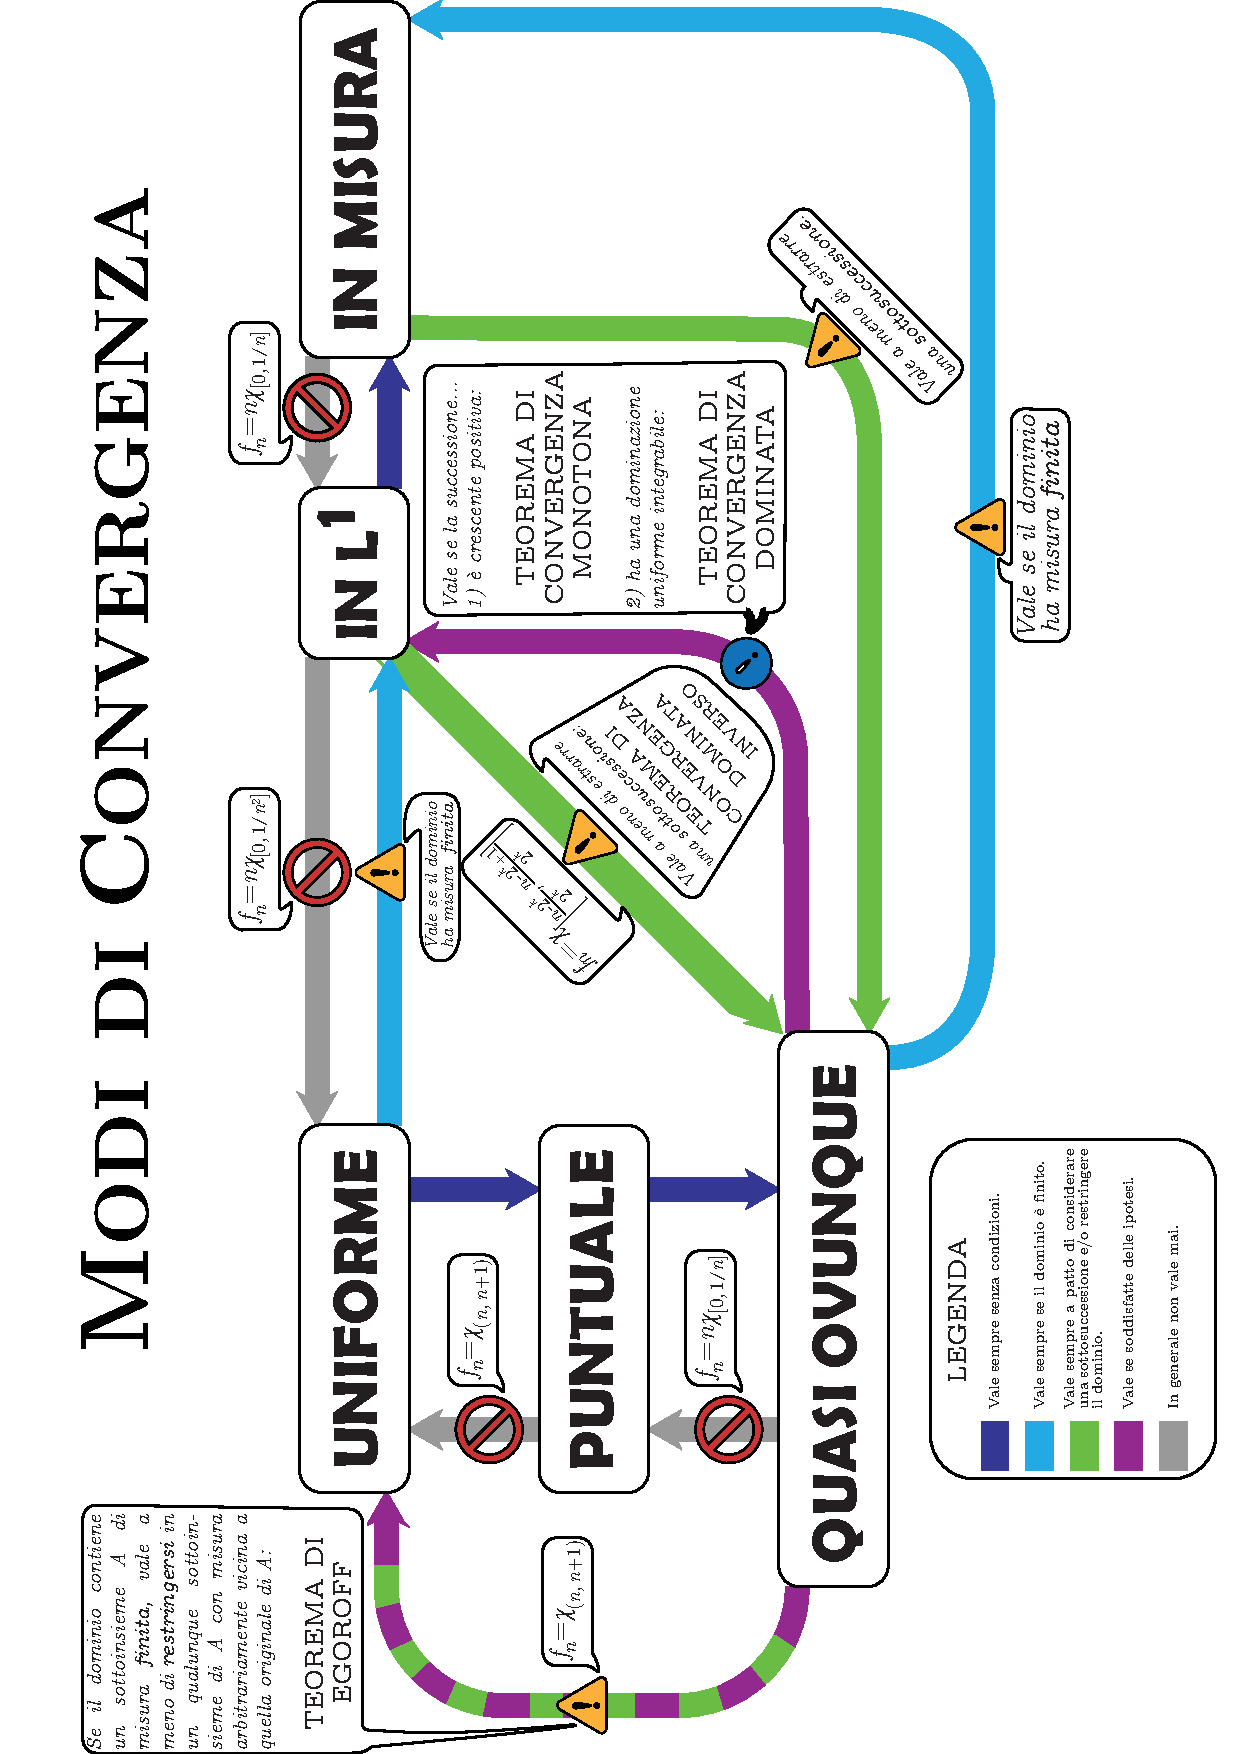
\includepdf{images/modiconvergenza2}
\newpage
\section{Passaggio al limite sotto segno di integrale}
\begin{center}
	\begin{tabular}{p{0.49\textwidth}p{0.49\textwidth}}
		\multicolumn{2}{c}{\textbf{Teoremi}} \\\hline
		\multicolumn{1}{c|}{
			 \textbf{Convergenza uniforme}} & \multicolumn{1}{c}{\textbf{Convergenza uniforme}}\\
		\multicolumn{1}{c|}{\textbf{(teoria di Riemann)}} &
			\multicolumn{1}{c}{\textbf{(teoria di Lebesgue)}} \\
		\multicolumn{1}{p{0.49\textwidth}|}{Siano $\funz{f_n,f}{\left[a,b\right]}{\realset},\ n\geq 1$ tali che
		\begin{enumerate}[label=(\alph*)]
			\item $f_n\in\mathcal{R}\left(\left[a,b\right]\right),\ \forall n\geq 1$.
			\item $f_n$ converge uniformemente a $f$ su $\left[a,b\right]$.
		\end{enumerate}
		} &
		Consideriamo lo spazio di misura $\left(X,\mathcal{M},\mu\right)$ e le funzioni $\funz{f_n,f}{X}{\complexset}$ tali che
		\begin{enumerate}[label=(\alph*)]
			\item $f_n\in L^{1}\left(\mu\right)$.
			\item $f_n$ converge uniformemente a $f$ su $X$.
			\item $\mu(X)<+\infty$.
		\end{enumerate}\\[-4mm]
		\multicolumn{1}{p{0.49\textwidth}|}{Allora
		\begin{enumerate}
			\item $f\in\mathcal{R}\left(\left[a,b\right]\right)$.
			\item Vale il \textbf{passaggio al limite sotto segno di integrale}:\newline
			\begin{tabular}[c]{c}
				$\displaystyle\lim_{n\to+\infty}\int_{a}^{b}\!\!\! f_n(x)dx=\int_{a}^{b}\!\!\!\lim_{n\to+\infty}f_n(x)dx$
			\end{tabular}
		\end{enumerate}} &
		Allora
		\begin{enumerate}
			\item $f\in L^{1}\left(\mu\right)$.
			\item $\displaystyle\lim_{n\to+\infty}\norm{f_n-f}_1=0$.
			\item Vale il \textbf{passaggio al limite sotto segno di integrale}:\newline
			\begin{tabular}[c]{c}
				$\displaystyle\quad\lim_{n\to+\infty}\int_X\!\!\! f_nd\mu=\int_X\!\!\lim_{n\to+\infty}f_nd\mu$
			\end{tabular}
		\end{enumerate} \\ \hline
		\multicolumn{2}{c}{\textbf{Vantaggi}}\\\hline
		\multicolumn{1}{p{0.49\textwidth}|}{
		\begin{itemize}
			\item È l'unico teorema sul passaggio di limite valido nella teoria di Riemann.
		\end{itemize}} &
		\begin{itemize}
			\item Vale su spazi di misura finita invece che solamente sugli intervalli finiti.
		\end{itemize} \\\hline
		\multicolumn{2}{c}{\textbf{Svantaggi}}\\\hline
		\multicolumn{1}{p{0.49\textwidth}|}{\begin{itemize}
			\item Richiede la convergenza uniforme.
			\item Vale solo per funzioni limitate.
			\item Vale solo su intervalli limitati.
		\end{itemize}} &
		\begin{itemize}
			\item Richiede la convergenza uniforme.
			\item Richiede l'integrabilità della successione.
			\item Vale solo su spazi di misura finita.
		\end{itemize}
	\end{tabular}
\end{center}
\newpage
\begin{center}
	\begin{tabular}{p{0.49\textwidth}p{0.49\textwidth}}
		\multicolumn{2}{c}{\textbf{Teoremi}} \\\hline
		\multicolumn{1}{c|}{\textbf{Convergenza monotona}} &
		\multicolumn{1}{c|}{\centering \textbf{Convergenza dominata}} \\
		\multicolumn{1}{p{0.49\textwidth}|}{
		Siano $\left(X,\mathcal{M},\mu\right)$ uno spazio di misura e $\funz{f_n,f}{X}{\left[0,+\infty\right]}$ con $n\geq 1$ tali che
		\begin{enumerate}[label=(\alph*)]
			\item $f_n$ sono misurabili.
			\item C'è convergenza puntuale:\newline
			$\displaystyle
				\lim_{n\to+\infty}f_n(x)=f(x),\ \forall x\in X$
			\item La successione di funzioni è crescente:
			$\displaystyle
				0\leq f_n(x)\leq f_{n+1}(x),\ \forall n\geq 1,\ \forall x\in X$
		\end{enumerate}
		} &
		Siano $\left(X,\mathcal{M},\mu\right)$ uno spazio di misura e $\funz{f_n,f}{X}{\complexset}$ con $n\geq 1$ tali che
		\begin{enumerate}[label=(\alph*)]
			\item 	$f_n$ sono misurabili.
			\item 	$\displaystyle \lim_{n\to+\infty}f_n(x)=f(x),\ \forall x\in X$
			\item 	Esiste una funzione $g\in \mathcal{L}^{1}\left(\mu\right)$ tale per cui\newline
			\begin{tabular}{c}
				$\displaystyle\quad \abs{f_n(x)}\leq g(x),\ \forall n\geq 1,\ \forall x\in X$	
			\end{tabular}
		\end{enumerate} \\[-4mm]
		\multicolumn{1}{p{0.49\textwidth}|}{Allora
		\begin{enumerate}
			\item $f$ è misurabile.
			\item Vale il \textbf{passaggio al limite sotto segno di integrale}:\newline
			\begin{tabular}{c}
				$\displaystyle\quad \lim_{n\to+\infty}\int_X\!\!\! f_nd\mu=\int_X\!\!\lim_{n\to+\infty}f_nd\mu$
			\end{tabular}
		\end{enumerate}} &
		Allora
		\begin{enumerate}
			\item $f\in L^{1}\left(\mu\right)$.
			\item $\displaystyle\lim_{n\to+\infty}\int_X\abs{f_n-f}d\mu=0$
			\item Vale il \textbf{passaggio al limite sotto segno di integrale}:\newline
			\begin{tabular}[c]{c}
				$\quad\displaystyle\lim_{n\to+\infty}\int_X\!\!\! f_nd\mu=\int_X\!\!\lim_{n\to+\infty}f_nd\mu$
			\end{tabular}
		\end{enumerate} \\\hline
		\multicolumn{2}{c}{\textbf{Vantaggi}} \\\hline
		\multicolumn{1}{p{0.49\textwidth}|}{\begin{itemize}
			\item Richiede solo la convergenza puntuale.
			\item Si può applicare anche con la convergenza \textbf{q.o.} purché la misura sia completa o la funzione limite $f$ è una funzione misurabile che coincide \textbf{q.o.} con il limite \textbf{q.o.} della successione.
			\item È sufficiente anche solamente supporre che la successione $f_n$ sia non decrescente su $X$ \textbf{q.o.}.
			\item Vale qualunque sia la misura di $X$.
		\end{itemize}} &
		\begin{itemize}
			\item Richiede solo la convergenza puntuale.
			\item Si può applicare anche con la convergenza \textbf{q.o.} e con la dominazione \textbf{q.o.} purché la misura sia completa o la funzione limite $f$ è una funzione misurabile che coincide \textbf{q.o.} con il limite \textbf{q.o.} della successione.
			\item Vale qualunque sia la misura di $X$.
			\item Vale per funzione a valori complessi.
		\end{itemize} \\\hline
		\multicolumn{2}{c}{\textbf{Svantaggi}} \\\hline
		\multicolumn{1}{p{0.49\textwidth}|}{\begin{itemize}
			\item Non vale per successioni decrescenti.
		\end{itemize}} &
		\begin{itemize}
			\item Richiede una dominazione della successione.
		\end{itemize}
	\end{tabular}
\end{center}
%% SVN info for this file
\svnidlong
{$HeadURL$}
{$LastChangedDate$}
{$LastChangedRevision$}
{$LastChangedBy$}

\chapter{Elenchi delle definizioni e dei teoremi}
\nocite{*}
\begin{multicols}{2}
	\listofdefines
\end{multicols}
\begin{center}
\rule{4cm}{0.4pt}
\end{center}
\begin{multicols}{2}
	\listoftheoremas
\end{multicols}
\begin{comment}
\end{comment}
%% SVN info for this file
\svnidlong
{$HeadURL$}
{$LastChangedDate$}
{$LastChangedRevision$}
{$LastChangedBy$}

\chapter{Pensieri e ringraziamenti}
\labelChapter{ringraziaments}

\begin{introduction}
‘‘\textbf{Lafayette}: Ehi, Napoleone! Direi che questa è la fine.\\
\textbf{Napoleone}: Un momento, il capo sono io! Lo dico io quando è la fine!\\
\textbf{[La parola \textsf{FINE} lo colpisce alla testa.]}\\
\textbf{Napoleone}: È la fine.''
\begin{flushright}
	\textscsl{Gli Aristogatti.}
\end{flushright}
\end{introduction}

\lettrine[findent=1pt, nindent=0pt]{A}{ Gennaio, quando} avevo concluso il Manualozzo\texttrademark\ di Analisi Matematica 3 mi ero detto ‘‘Bene, ho scritto tre Manualozzi\texttrademark\. Uno per anno. Tre è un bel numero per smettere.''.\\
Eppure, all'inizio del nuovo semestre, mi fu gentilmente chiesto di farne uno nuovo - per di più per un corso come Fisica II, la bestia nera di ogni matematico. Chiaramente mi rifiutai: l'esperienza dei Manualozzi\texttrademark\ è stata bella, ma mo' basta! Ma evidentemente la mia dipendenza da Manualozzi\texttrademark\ ha preso il sopravvento, perché alla fine ne state leggendo uno. Sigh. Menomale che Elisa mi ha aiutato sbobinando le lezioni - anche se mi meraviglio ogni volta che sia in grado di farlo già in \LaTeX\ mentre il prof spiega.\\
\newline
\noindent Il testo che avete di fronte è in realtà una versione \textit{incompleta} di quella che inizialmente doveva essere: per questioni di tempo e di salute, non son riuscito a lavorare alla parte dedicata alle onde, né quella di relatività e quantistica. Se troverò mai tempo di scrivere una nuova edizione cercherò almeno di trattare le onde.\\
Ciò nonostante, credo che questo sarà davvero l'ultimo Manualozzo\texttrademark. Un po' poeticamente, concludo questa esperienza come ho iniziato: con un argomento di ambito fisico. Anche se so già che ben presto mi rimangerò queste parole.\\
\newline
\noindent Essendo anche oramai finita la Triennale, vorrei utilizzare questo spazio per ringraziare e salutare le tante persone con cui sono venuto in contatto durante questi anni e che, chi di più, chi di meno, hanno influenzato la mia vita universitaria. Ciò nonostante, non penso di dilungarmi troppo: ho già scritto quasi 300 pagine in \LaTeX\ e se proprio posso evitarne altre non mi dispiacerebbe farlo.\\
\newline
A Elisa Antuca, a cui va il mio più sentito ringraziamento per l'aiuto che mi ha dato non solo in questo Manualozzo\texttrademark, ma anche per tutti quelli precedenti. Per essere un pinguino ci sa fare con \LaTeX.\\
A Francesca Colombo, che da vera amica con il suo essere solare mi ha portato un po' di luce nei momenti più bui. E apprezzo davvero il suo magico potere di convincermi a non lavorare troppo, non so come faccia.\\
A Guido Buffa, che con la simpatia - e sì, anche con il suo sarcasmo - sono sicuro che se si desse alla \textit{stand up comedy} diventerebbe famoso... e starei in prima fila a ridere di buon gusto. Purtroppo alla fine non sono diventato un membro produttivo della società a causa sua e di Farming Simulator, purtuttavia non mi lamento.\\
A Julian Kerpaci, che con la sua vivacità e il suo sorriso in faccia mi rallegra spesso la giornata. Forse mi rallegra anche il fatto di averlo battuto al Fantacalcio. \\
A Samuele Corsato, che fra poco potrebbe persino superarmi in \LaTeX. {\small Forse.} {\tiny Ti tengo d'occhio.}\\
A Marco Lugarà, che non è assolutamente colui che mi spinse a scrivere questo Manualozzo\texttrademark. {\small Ogni tanto dovrei dirgli di no, mannaggia a me.}\\
A Matteo Cagnotti, Emiliano Colla, Lorenzo Ferrara, Andrea Scalenghe, Charif El Gataa, Matteo Bracco, Chiara Comoglio, ma anche a Matilda Urani, Andrea Natale, Pietro Raviola, Riccardo Ponte, Francesco Ruatta, Zoe Wynants, Eugenio del Nero, Orazio Nicolosi, He Xiaohui, Davide Miolano, Lisa Galvagni - insomma, a tutto il \textit{Chen Fanpage \& friends} - e a tutta la gente simpatica che ho conosciuto in tre anni di università: avrei tante cose da dire, ma il margine della pagina è troppo stretto per farlo.\\
A Elena Maserati, che devo ancora capire come fai preferire Fisica a Matematica, tsk. Prima o poi ti farò piacere la Matematica, Diofà!
\begin{flushright}
	\textcolor{redill}{\href{https://www.youtube.com/watch?v=QXPZG9Gv75M}{\textscsl{See you space Manualozzo...}}}
\end{flushright}
\vfill
\begin{center}
	\begin{frame}{}
		\animategraphics[loop,autoplay,width=0.5\linewidth]{7}{images/meme/rick-}{0}{93}
	\end{frame}
\end{center}
\vspace{5pt}
\begin{center}
{\scriptsize Una piccola curiosità: questa immagine e anche quella di copertina sono state create interamente dall'intelligenza artificiale \textbf{DALL·E 2} basandosi l'input \textit{``A surrealist painting of a magnet in the style of The Treachery of Images by René Magritte''}.\\
\textit{Il tradimento delle immagini}, huh... chissà se questa immagine mi tradirà.}
\end{center}
%\backmatter
%% SVN info for this file
\svnidlong
{$HeadURL$}
{$LastChangedDate$}
{$LastChangedRevision$}
{$LastChangedBy$}

\RaggedRight
\printbibliography
\printindex

\end{document}
